% ******************************* PhD Thesis Template **************************
% Please have a look at the README.md file for info on how to use the template

\documentclass[a4paper,12pt,times,numbered,print]{Classes/PhDThesisPSnPDF}

% ******************************************************************************
% ******************************* Class Options ********************************
% *********************** See README for more details **************************
% ******************************************************************************

% `a4paper'(The University of Cambridge PhD thesis guidelines recommends a page
% size a4 - default option) or `a5paper': A5 Paper size is also allowed as per
% the Cambridge University Engineering Deparment guidelines for PhD thesis
%
% `11pt' or `12pt'(default): Font Size 10pt is NOT recommended by the University
% guidelines
%
% `oneside' or `twoside'(default): Printing double side (twoside) or single
% side.
%
% `print': Use `print' for print version with appropriate margins and page
% layout. Leaving the options field blank will activate Online version.
%
% `index': For index at the end of the thesis
%
% `draftclassic': For draft mode without loading any images (same as draft in book)
%
% `draft': Special draft mode with line numbers, images, and water mark with
% timestamp and custom text. Position of the text can also be modified.
%
% `abstract': To generate only the title page and abstract page with
% dissertation title and name, to submit to the Student Registry
%
% `chapter`: This option enables only the specified chapter and it's references
%  Useful for review and corrections.
%
% ************************* Custom Page Margins ********************************
%
% `custommargin`: Use `custommargin' in options to activate custom page margins,
% which can be defined in the preamble.tex. Custom margin will override
% print/online margin setup.
%
% *********************** Choosing the Fonts in Class Options ******************
%
% `times' : Times font with math support. (The Cambridge University guidelines
% recommend using times)
%
% `fourier': Utopia Font with Fourier Math font (Font has to be installed)
%            It's a free font.
%
% `customfont': Use `customfont' option in the document class and load the
% package in the preamble.tex
%
% default or leave empty: `Latin Modern' font will be loaded.
%
% ********************** Choosing the Bibliography style ***********************
%
% `authoryear': For author-year citation eg., Krishna (2013)
%
% `numbered': (Default Option) For numbered and sorted citation e.g., [1,5,2]
%
% `custombib': Define your own bibliography style in the `preamble.tex' file.
%              `\RequirePackage[square, sort, numbers, authoryear]{natbib}'.
%              This can be also used to load biblatex instead of natbib
%              (See Preamble)
%
% **************************** Choosing the Page Style *************************
%
% `default (leave empty)': For Page Numbers in Header (Left Even, Right Odd) and
% Chapter Name in Header (Right Even) and Section Name (Left Odd). Blank Footer.
%
% `PageStyleI': Chapter Name next & Page Number on Even Side (Left Even).
% Section Name & Page Number in Header on Odd Side (Right Odd). Footer is empty.
%
% `PageStyleII': Chapter Name on Even Side (Left Even) in Header. Section Number
% and Section Name in Header on Odd Side (Right Odd). Page numbering in footer


% ********************************** Preamble **********************************
% Preamble: Contains packages and user-defined commands and settings
% ******************************************************************************
% ****************************** Custom Margin *********************************

% Add `custommargin' in the document class options to use this section
% Set {innerside margin / outerside margin / topmargin / bottom margin}  and
% other page dimensions
\ifsetCustomMargin
  \RequirePackage[left=37mm,right=30mm,top=35mm,bottom=30mm]{geometry}
  \setFancyHdr % To apply fancy header after geometry package is loaded
\fi

% *****************************************************************************
% ******************* Fonts (like different typewriter fonts etc.)*************

% Add `customfont' in the document class option to use this section

\ifsetCustomFont
  % Set your custom font here and use `customfont' in options. Leave empty to
  % load computer modern font (default LaTeX font).
  %\RequirePackage{helvet}

  % For use with XeLaTeX
    \setmainfont[
      Path              = cambria/,
      %Extension         = .ttf,
      UprightFont = Cambria.ttf,
      BoldFont = Cambria_Bold.ttf, % Linux Libertine O Regular Semibold
      ItalicFont = Cambria_Italic.ttf,
      BoldItalicFont = Cambria_Bold_Italic.ttf, % Linux Libertine O Regular Semibold Italic
    ]
    {Cambria.ttf}
    % load font from system font
    %\newfontfamily\libertinesystemfont{Linux Libertine O}
\fi

% *****************************************************************************
% **************************** Custom Packages ********************************

% ************************* Algorithms and Pseudocode **************************

%\usepackage{algpseudocode}


% ********************Captions and Hyperreferencing / URL **********************

% Captions: This makes captions of figures use a boldfaced small font.
%\RequirePackage[small,bf]{caption}

\RequirePackage[labelsep=space,tableposition=top]{caption}
\renewcommand{\figurename}{Fig.} %to support older versions of captions.sty

\usepackage{paralist}
\usepackage[inline]{enumitem}
\usepackage[super]{nth}
% *************************** Graphics and figures *****************************

%\usepackage{rotating}
%\usepackage{wrapfig}

% Uncomment the following two lines to force Latex to place the figure.
% Use [H] when including graphics. Note 'H' instead of 'h'
%\usepackage{float}
%\restylefloat{figure}

% Subcaption package is also available in the sty folder you can use that by
% uncommenting the following line
% This is for people stuck with older versions of texlive
%\usepackage{sty/caption/subcaption}
\usepackage{subcaption}
\usepackage{graphicx}

% ********************************** Tables ************************************
\usepackage{booktabs} % For professional looking tables
\usepackage{multirow}

%\usepackage{multicol}
%\usepackage{longtable}
%\usepackage{tabularx}


\usepackage{bibentry} % to support list of publication
\usepackage{natbib} 
\nobibliography*

% *********************************** SI Units *********************************
\usepackage{siunitx} % use this package module for SI units


% *********************************** Using glossaries *********************************
% Load the package
\usepackage[toc,acronym, nonumberlist]{glossaries}
% Generate the glossary
\makeglossaries
% \makenoidxglossaries % To support list of glossary sorting
\setacronymstyle{long-short}
\newacronym{lisp}{LISP}{Locator/Identifier Separation Protocol}
\newacronym{eid}{EID}{Endpoint IDentifier}
\newacronym{rloc}{RLOC}{Routing LOCator}
\newacronym{itr}{ITR}{Ingress Tunnel Router}
\newacronym{etr}{ETR}{Egress Tunnel Router}
\newacronym{xtr}{xTR}{Ingress  Egress Tunnel Router}
\newacronym{pitr}{PITR}{Proxy Ingress Tunnel Router}
\newacronym{petr}{PETR}{Proxy Egress Tunnel Router}
\newacronym{pxtr}{PxTR}{Proxy Ingress  Egress Tunnel Router}
\newacronym{mr}{MR}{Map-Resolver}
\newacronym{ms}{MS}{Map-Server}
\newacronym{bgp}{BGP}{Border Gateway Protocol}
\newacronym{dfz}{DFZ}{Defaut Free Zone}
\newacronym{dns}{DNS}{Domain Name System}
\newacronym{sip}{SIP}{Session Initiation Protocol}
\newacronym{mds}{MDS}{Mapping Distribution System}
\newacronym{lispalt}{LISP+ALT}{LISP Alternative Logical Topology}
\newacronym{lispddt}{LISP-DDT}{LISP Delegated Database Tree}
\newacronym{lispmn}{LISP-MN}{LISP Mobile Node}
\newacronym{lispsn}{LISP-SN}{LISP Stationary Node}
\newacronym{smr}{SMR}{Solicit-Map-Request}
\newacronym{lrloc}{LRLOC}{Local RLOC}
\newacronym{cn}{CN}{Correspondent Node}
\newacronym{mn}{MN}{Mobile Node}
\newacronym{vm}{VM}{Virtual Machine}
\newacronym{sdn}{SDN}{Software Defined Network}
\newacronym{nfv}{NFV}{Network Functions Virtualization}
\newacronym{vp}{VP}{Vantage Point}
\newacronym{rtt}{RTT}{Round-Trip Time}
\newacronym{arpanet}{ARPANET}{Advanced Research Projects Agency Network}
\newacronym{lig}{LIG}{LISP Internet Groper}
\newacronym{rig}{RIG}{LISP-DDT Referral Internet Groper}

% ******************************* Line Spacing *********************************

% Choose linespacing as appropriate. Default is one-half line spacing as per the
% University guidelines

% \doublespacing
% \onehalfspacing
% \singlespacing


% ************************ Formatting / Footnote *******************************

% Don't break enumeration (etc.) across pages in an ugly manner (default 10000)
%\clubpenalty=500
%\widowpenalty=500

%\usepackage[perpage]{footmisc} %Range of footnote options


% *****************************************************************************
% *************************** Bibliography  and References ********************

%\usepackage{cleveref} %Referencing without need to explicitly state fig /table

% Add `custombib' in the document class option to use this section
\ifuseCustomBib
   \RequirePackage[square, sort, numbers, authoryear]{natbib} % CustomBib

% If you would like to use biblatex for your reference management, as opposed to the default `natbibpackage` pass the option `custombib` in the document class. Comment out the previous line to make sure you don't load the natbib package. Uncomment the following lines and specify the location of references.bib file

%\RequirePackage[backend=biber, style=numeric-comp, citestyle=numeric, sorting=nty, natbib=true]{biblatex}
%\bibliography{References/references} %Location of references.bib only for biblatex

\fi

% changes the default name `Bibliography` -> `References'
\renewcommand{\bibname}{References}


% ******************************** Roman Pages *********************************
% The romanpages environment set the page numbering to lowercase roman one
% for the contents and figures lists. It also resets
% page-numbering for the remainder of the dissertation (arabic, starting at 1).

\newenvironment{romanpages}{
  \setcounter{page}{1}
  \renewcommand{\thepage}{\roman{page}}}
{\newpage\renewcommand{\thepage}{\arabic{page}}}


% ******************************************************************************
% ************************* User Defined Commands ******************************
% ******************************************************************************

% *********** To change the name of Table of Contents / LOF and LOT ************

%\renewcommand{\contentsname}{My Table of Contents}
%\renewcommand{\listfigurename}{My List of Figures}
%\renewcommand{\listtablename}{My List of Tables}


% ********************** TOC depth and numbering depth *************************

\setcounter{secnumdepth}{2}
\setcounter{tocdepth}{2}


% ******************************* Nomenclature *********************************

% To change the name of the Nomenclature section, uncomment the following line

%\renewcommand{\nomname}{Symbols}


% ********************************* Appendix ***********************************

% The default value of both \appendixtocname and \appendixpagename is `Appendices'. These names can all be changed via:

%\renewcommand{\appendixtocname}{List of appendices}
%\renewcommand{\appendixname}{Appndx}

% *********************** Configure Draft Mode **********************************

% Uncomment to disable figures in `draftmode'
%\setkeys{Gin}{draft=true}  % set draft to false to enable figures in `draft'

% These options are active only during the draft mode
% Default text is "Draft"
%\SetDraftText{DRAFT}

% Default Watermark location is top. Location (top/bottom)
%\SetDraftWMPosition{bottom}

% Draft Version - default is v1.0
%\SetDraftVersion{v1.1}

% Draft Text grayscale value (should be between 0-black and 1-white)
% Default value is 0.75
%\SetDraftGrayScale{0.8}


% ******************************** Todo Notes **********************************
%% Uncomment the following lines to have todonotes.

\ifsetDraft
	\usepackage[colorinlistoftodos,prependcaption,textsize=tiny]{todonotes}
	\newcommand{\qsong}[1]{\todo[inline, linecolor=red,backgroundcolor=red!25,bordercolor=red]{#1}}
	\newcommand{\improve}[1]{\todo[size=\small,inline,color=green!40]{#1}}
\else
	\newcommand{\qsong}[1]{}
	\newcommand{\yli}[1]{}
	\newcommand{\listoftodos}{}
\fi

% Example todo: \mynote{Hey! I have a note}

\newcommand{\yue}[1]{\textcolor{blue}{(\textbf{[Yue] }\textit{#1}})}
\newcommand{\qs}[1]{\textcolor{red}{(\textbf{[qs] }\textit{#1}})}

% ************************ Thesis Information & Meta-data **********************
% Thesis title and author information, refernce file for biblatex
% ************************ Thesis Information & Meta-data **********************
%% The title of the thesis
\title{Future Internet Services based on LISP Technology}
%\texorpdfstring is used for PDF metadata. Usage:
%\texorpdfstring{LaTeX_Version}{PDF Version (non-latex)} eg.,
%\texorpdfstring{$sigma$}{sigma}

%% Subtitle (Optional)
%\subtitle{Using the CUED template}

%% The full name of the author
\author{Yue LI}

%% Department (eg. Department of Engineering, Maths, Physics)
\dept{Department of INFRES}

%% University and Crest
\university{Telecom Paristech}
% Crest minimum should be 30mm.
%\crest{
\includegraphics[width=0.2\textwidth]{University_Crest}}
%% Use this crest, if you are using the college crest
%% Crest long miminum should be 65mm
%\crest{
\includegraphics[width=0.45\textwidth]{University_Crest_Long}}

%% College shield [optional] 
% Crest minimum should be 30mm.
%\collegeshield{
\includegraphics[width=0.2\textwidth]{CollegeShields/Kings}}

% Supervisor (optional)
% for multiple supervisors, append each supervisor with the \newline command
% \supervisor{\textbf{Prof. A.B. Supervisor\newline
% Prof. C.D. Supervisor\newline
% Prof. E.F. Supervisor\newline
% Prof. G.H. Supervisor}}

%% Supervisor Role (optional) - Supervisor (default) or advisor
% \supervisorrole{\textbf{Supervisors: }}
%% if no title is desired:
% \supervisorrole{}

%% Advisor (optional)
%% for multiple advisors, append each advisor with the \newline command
%\advisor{Advisor 1\newline
%Advisors 2\newline
%Advisor 3\newline
%Advisor 4}

%% Advisor Role (optional) - Advisor (default) or leave empty
% \advisorrole{Advisors: }
%% if no title is required
% \advisorrole{}

%% You can redefine the submission text:
% Default as per the University guidelines:
% ``This dissertation is submitted for the degree of''
%\renewcommand{\submissiontext}{}

%% Full title of the Degree
\degreetitle{Doctor of Philosophy}

%% College affiliation (optional)
%\college{Computer and Networking}

%% Submission date
%Default is set as {\monthname[\the\month]\space\the\year}
\degreedate{}

%% Meta information
%\subject{LaTeX} \keywords{{LaTeX} {PhD Thesis} {Engineering} {University of %Cambridge}}


% ***************************** Abstract Separate ******************************
% To printout only the titlepage and the abstract with the PhD title and the
% author name for submission to the Student Registry, use the `abstract' option in
% the document class.

\ifdefineAbstract
 \pagestyle{empty}
 \includeonly{Declaration/declaration, Abstract/abstract}
\fi

% ***************************** Chapter Mode ***********************************
% The chapter mode allows user to only print particular chapters with references
% Title, Contents, Frontmatter are disabled by default
% Useful option to review a particular chapter or to send it to supervisior.
% To use choose `chapter' option in the document class

%\ifdefineChapter
% \includeonly{Chapter6/chapter6}
%\fi

% ******************************** Front Matter ********************************
\begin{document}\sloppy

\frontmatter

\begin{titlepage}
  \maketitle
\end{titlepage}


%% ******************************* Thesis Dedidcation ********************************

\begin{dedication} 

I would like to dedicate this thesis to my loving parents \dots

\end{dedication}
%% ******************************* Thesis Declaration ***************************

\begin{declaration}

%I hereby declare that except where specific reference is made to the work of 
%others, the contents of this dissertation are original and have not been 
%submitted in whole or in part for consideration for any other degree or 
%qualification in this, or any other university. This dissertation is my own 
%work and contains nothing which is the outcome of work done in collaboration 
%with others, except as specified in the text and Acknowledgements. This 
%dissertation contains fewer than 65,000 words including appendices, 
%bibliography, footnotes, tables and equations and has fewer than 150 figures.

% Author and date will be inserted automatically from thesis.tex \author \degreedate

\end{declaration}


% ************************** Thesis Acknowledgements **************************

\begin{acknowledgements}      


And I would like to acknowledge ...


\end{acknowledgements}

% \begin{publications}

\begin{itemize}
	\item \bibentry{yue2016stability}
	\item \bibentry{li2016using}
	\item \bibentry{li2016performance}
	\item \bibentry{li2017lisp}
	\item \bibentry{Li2017}
\end{itemize}

\end{publications}
% ************************** Thesis Abstract *****************************
% Use `abstract' as an option in the document class to print only the titlepage and the abstract.
\begin{abstract}
The \emph{\acrfull{lisp}} is proposed in 2006 to initially address nowadays' Internet scalability issues. It is based on a map-encap mechanism to split \emph{who} (\emph{\acrfull{eid}}) and \emph{where} (\emph{\acrfull{rloc}}) of the current IP address. A new network entity called the (\emph{\acrfull{mds}}) is introduced to associate \acrshort{rloc} with \acrshort{eid}. \acrshort{lisp} leverages on a proxy (\emph{\acrfull{pxtr}}) to communicate with the legacy Internet. Thanks to the Loc/ID separation paradigm, \acrshort{lisp} also brings some other benefits to the future Internet, such as the seamless mobility. Although \acrshort{lisp} is currently under standardization in IETF and is deployed in the wild by two testbeds at the same time, it is still young. It lacks the thorough measurement works to show its performance in the large-scale realistic networks and to improve itself. In this dissertation, we assess \acrshort{lisp} from the different aspects :
\begin{inparaenum}[(i)]
	\item the measurements on the \acrshort{mds}, including: evaluating its performance, and proposing a comprehensive monitor to supervise it;
	\item the assessment of \acrshort{pxtr}.
	\item the evaluation of \acrshort{lisp} mobility, comprising: numerically analyzing in different scenarios, and implementing \acrshort{lisp} mobility extensions on an existing simulator.
\end{inparaenum}

We continuously measured the \acrshort{mds} for seventeen days. The results show that it is stable and consistent over most of time. Nevertheless, instability and inconsistency are observed although they are rare events. We define a new taxonomy to classify them so to facilitate the deeper analysis. As these instability and inconsistency have never been observed, we propose a more comprehensive LISP monitoring architecture to dynamically supervise the whole \acrshort{mds}. After one full month of testing, our proposed monitor provides more mapping information, and can show the \acrshort{mds} performance by various metrics. We also evaluate \acrshort{lisp} interworking performance with legacy Internet by conducting two experiments in the different years. Both results show that \acrshort{lisp} is stable although the stretch of \acrshort{pxtr} is introduced. The \acrshort{pxtr} brings the negative effects for the short trips, but can be ignored for the intercontinental long-distance transmission. Besides, the position of \acrshort{pxtr} either near to the sources or the destinations can decrease the latency a lot. Moreover, we numerically analyze the mobility performance of \acrshort{lisp} in three scenarios. We calculate the lower bounds of handover for the different components implementing \acrshort{lisp}. Each scenario has its own advantages and shortcomings. Besides, to facilitate the researchers to verify their proposals or test the new features on \acrshort{lisp} mobility, we implement \acrshort{lisp} mobility extensions under ns-3.27 on an existing simulator.
\end{abstract}

% *********************** Adding TOC and List of Figures ***********************

\tableofcontents

\listoffigures

\listoftables


% \printnomenclature[space] space can be set as 2em between symbol and description
%\printnomenclature[3em]

%\printnomenclature
\glsaddall
\printglossary[type=\acronymtype,title=List of Abbreviation]
% \printnoidxglossaries

% ******************************** Main Matter *********************************
\mainmatter

%*******************************************************************************
%*********************************** First Chapter *****************************
%*******************************************************************************

\chapter{Introduction}  %Title of the First Chapter
\label{cha:intro}

% **************************** Define Graphics Path **************************
\ifpdf
    \graphicspath{{Chapter1/Pics/Raster/}{Chapter1/Pics/PDF/}{Chapter1/}}
\else
    \graphicspath{{Chapter1/Pics/Vector/}{Chapter1/}}
\fi



%-< SECTION >--------------------------------------------------------------------
\section{Motivations}
\label{sec:intro_motivations}
%\begin{itemize}[noitemsep,topsep=0pt]
%    \item Nowadays Internet has scalability issue and lacks of flexibility.
%    \item Due to Internet problems, LISP is proposed.
%    \item State LISP current status.
%    \item As LISP is still in infancy, which kinds of works are need to do to move LISP forward.
%\end{itemize}

%-< FIGURE >--------------------------------------------------------------------
\begin{figure}[t]
	\centering
	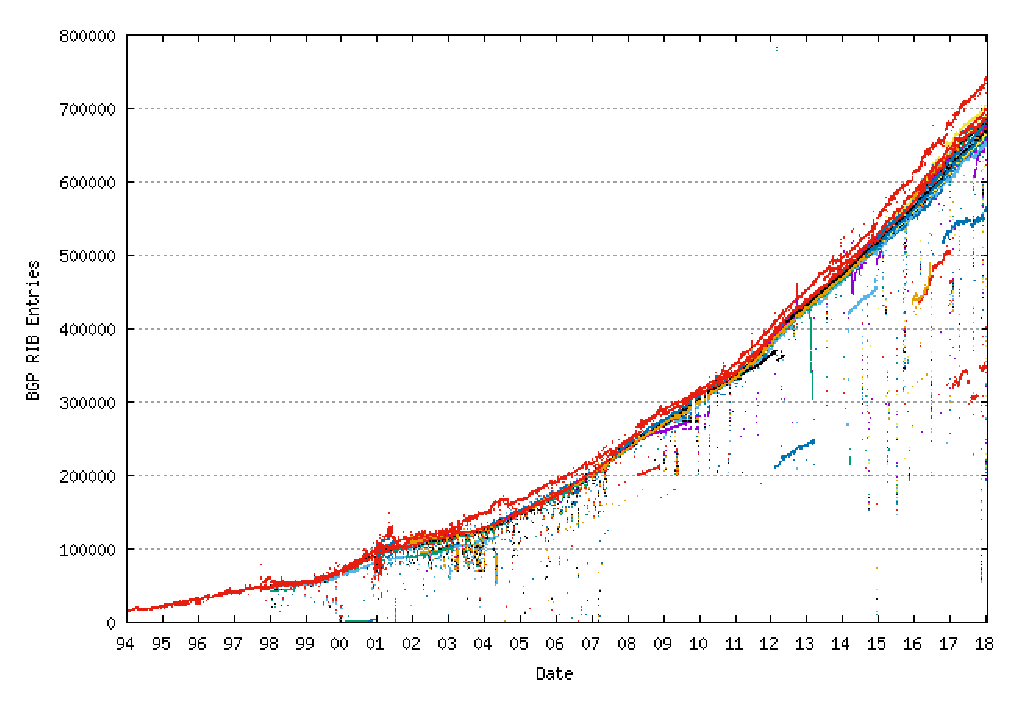
\includegraphics[width=0.8\textwidth]{Pics/Growth_BGP_Table.eps}
	\caption{Growth of the BGP Table - 1994 to Present}
	\label{Growth_BGP_Table}
\end{figure}
%-< END FIGURE >--------------------------------------------------------------------
Since the \acrshort{arpanet} (\acrlong{arpanet}) emerged in 1966~\cite{marill1966toward}, the Internet has obtained significant achievements over the last fifty years and developed very fast. Until the beginning of 2018, the Internet users in the world achieves 3.82 billions, i.e., around 40\% of the world population has an Internet connection today~\cite{InternetLiveStats}. Moreover, we come into the era of the mobile Internet. According to the latest research~\cite{SmartInsights}, the number of global mobile users has been higher than that of desktop since 2014. Although having a huge success, today's Internet is suffering the overloading of IP address semantics, which results in many shortcomings in the application landscape~\cite{feng2017locator}. As in the current TCP/IP protocol stack, the IP address serves both as the \emph{who} to identify the host and the \emph{where} to indicate the attachment point in the network topology, leading to a serious routing scalability problem. As shown in Fig.~\ref{Growth_BGP_Table}, the BGP table size, which is the number of IP prefixes in the \acrshort{bgp} (\acrlong{bgp}) routing table of \acrshort{dfz} (\acrlong{dfz}) routers, has grown at a super-linear rate in recent years. After full use of IPv6, the routing scalability issue will be aggravated, since it has much larger addressing space than IPv4. Maintaining such routing table is very cumbersome. Particular, once a site changes its routing information, all the routers need to update, which causes a huge BGP churn. In addition, frequent routing information updates result in the increasing of convergence time and packet loss rates.

To cope with the current Internet scalability problems, the Loc/ID separation paradigm is proposed, which separates the single IP addressing space into two orthogonal spaces. Many solutions based on this mechanism are proposed, which can be classified into two catalogs: \emph{Host-based} and \emph{Network-based}. The former one needs to modify the host stack. The representative architectures are: HIP (Host Identity Protocol)~\cite{nikander2010host}~\cite{Moskowitz2017host}~\cite{moskowitz2015host}, Six/One~\cite{vogt2007six}, SHIM6 (Site Multihoming by IPv6 Intermediation)~\cite{garcia2010shim6}~\cite{nordmark2009shim6}, ILNP (Identifier-Locator Network Protocol)~\cite{bhatti2012identifier}~\cite{atkinson2010evolving}, and LNA (Layered Naming Architecture)~\cite{balakrishnan2004layered}. The network-based approach needs to update the routers, and the representative proposals are: GSE (Global, Site, and End-system address elements)~\cite{o2006gse}, LISP (Locator/ID Separation Protocol)~\cite{rfc6830}, and TIDR (Tunneled Inter-domain Routing)~\cite{adan2006tunneled}. Among them, LISP is outstanding by its relatively comprehensive network systems in both control and data planes. % This characterization promotes the standardization, production and industrtialization of LISP. 
LISP was initially proposed by Cisco in 2006 and has an exclusive IETF WG since 2009. % which guarantees LISP can be actively under developed.

The key philosophy of LISP is to separate the IP addressing space into two sub-spaces: the \emph{Routing LOCators} (RLOCs) and the \emph{Endpoint IDentifiers} (EIDs). End-to-end communication is based on EIDs, which in an intra-domain context means just to performing conventional routing and forwarding. On the contrary, for inter-domain end-to-end communication, RLOCs are used for routing and forwarding. To this end, LISP does a map-and-encap operation, first mapping EIDs to RLOCs (through a DNS-like on-demand mapping system~\cite{lispALTPourri}) and then encapsulating the original packet so to use RLOCs on the outer header. Internetworking between LISP and non-LISP networks is performed through two types of proxies~\cite{rfc6832}: \emph{Proxy Ingress Tunnel Routers} (PITRs) and \emph{Proxy Egress Tunnel Routers} (PETRs). They are collectively denoted by \emph{PxTR}. PITRs advertise in the BGP  routing infrastructure the EID-prefix space on behalf of the LISP sites, so that non-LISP sites can reach them. % In this way PITRs attract the traffic from non-LISP sites, which simply send packets with destination EID as destination IP address. Subsequently the PITR performs LISP encapsulation and forward the packets to the destination. 
PETRs are used as exit points from LISP sites when the destination is not an EID in a LISP site. % Hence, PETRs decapsulate the LISP-encapsualted packets received from LISP-sites and forwards them in the legacy Internet. 
With help of this detaching mechanism, LISP is able to improve the Internet routing scalability, enable enhanced inter-domain traffic engineering, lightweight multi-tenant carrier-grade VPN, and \acrshort{vm}s mobility in Data-Centers~\cite{saucez2012designing}.

% LISP introduces several benefits to the Internet architecture. Many companies and academic institutes participate into LISP development, so that the standardizations and research publications about LISP are continuously came out in the recent years. Besides, two large scale experimental LISP platforms are deployed on the world respectively in 2008 and 2015. All the efforts, however, are mainly about the description of LISP architectures, implementations, extensions and applications. It lacks of the comprehensive LISP measurement works from the various aspects. In addition, LISP remains a relatively recent technology and these large scale flexible platforms are still in an early stage, it needs plenty of large scale experiments to obtain realistic LISP experiences ont only further improve the performance of two platforms, but ultimately to provide feedback to the community on how to move the LISP technology forward.

As LISP is a promising technology that brings many benefits to the future Internet, it attracts the attention from both academic and industrial world. Many companies, universities and research institutes are now involved in the development of LISP. Hence, the related standardization and researches are very active. In terms of deployment, two large-scale experimental LISP platforms: LISP Beta Network and LISP-Lab platform are deployed on the world respectively in 2008 and 2015. Up to date, all the efforts are mainly about the theoretic or simulation-based performance analysis, description of LISP architectures, implementations, extensions, applications and so on. However, it lacks of the comprehensive measurement works for LISP technology itself. These performance measurements work will give the research community a clear view about the LISP performance, reveal the points that can be improved, indicate possible research directions, and improve the performance of two platforms. Thus, the large-scale measurements in realistic networks are of paramount importance for the LISP development.

%-< SECTION >--------------------------------------------------------------------
\section{Contributions}
\label{sec:intro_contributions}
With the goal of evaluating LISP from the different views, in this dissertation we aim at answering the following research questions, which have not been tackled before:
\begin{enumerate}[noitemsep,topsep=0pt]
	\item Mapping system is essential in LISP, because it decides where the packets will be routed. Thus, does it always provide the identical mapping information for the same destination? Do all of the resolvers of the mapping system offer the same response at the same time? Does the mapping information replies keep consistent if we query them from the different \acrfull{vp}s?
	
	We continuously measured LISP Beta Network for seventeen days. Measurements show that the LISP mapping system is stable over most of time. The replies from the different \acrshort{mr}s and \acrshort{vp}s are also mostly consistent. Nevertheless, instability and inconsistency are observed although they are rare events. We define a new taxonomy to classify these instability and inconsistency so to facilitate the deeper analysis. This work is published in WNM~\cite{yue2016stability}.
	
	\item As the results of the last question show that there exists inconsistency between the \acrshort{mr}s and \acrshort{vp}s, is it possible to implement a comprehensive monitor so to simultaneously supervise the whole mapping system and all the resolvers?
	
	We propose a dynamic LISP monitoring architecture, namely LISP-Views, so to deepen the understandings on LISP and to ease day-to-day operations and troubleshooting. After one full month monitoring to the whole LISP mapping system of two platforms, it demonstrates that LISP-Views provides % more information by discovering more mapping information from all \acrshort{mr}s and more 
	the complete mapping information. Furthermore, with our proposed monitoring platform, more mapping system performance metrics such as reliability, latency, and configuration issues can be assessed, which helps for further LISP improvements. This work is published in ITC~\cite{li2017lisp}.
	
	\item By using proxy approach to communicate with the legacy Internet, a stretch in the path is introduced. Thus, how much is it in the real world performance when the platforms integrate with the legacy Internet? Under which conditions such stretch has an important impact on the performance? Conversely, under which situation such overhead is so small that it can be ignored? 
	
	To evaluate LISP interworking performance with legacy Internet, we conduct two times experiments. The results of twice experiments are coherent. Both of them show that LISP is stable although the stretch is introduced due to the using of proxy. We find that the proxy indeed introduces the negative effects for the destinations located in Europe and America, but can be ignored for the intercontinental long-distance transmission to Asia destinations. Besides, we observe that the position of proxy is very important. It either near to the sources or the destinations can decrease the latency a lot. % Further, the performance of LISP-Lab PxTR is more reliable than the one of LISP Beta Network. 
	This work is published in INFOCOM Student workshop~\cite{li2016using}, ACM SIGCOMM Student workshop~\cite{li2016performance}, and Elsevier Computer Networks~\cite{Li2017}.
	
	\item As LISP separates the identifier and the topological attachment point from the traditional IP address, it is able to maintain the communication between two hosts during the handover without interruption. LISP can be implemented on the border routers or the terminals or even both of them. Thus, which network element supports LISP showing a better performance, i.e., having a shorter handover delay or introducing less overhead during the mobility? What are the advantages and shortcomings of each case? Leveraging on which simulator can we verify?
	
	To explore the mobility performance of the LISP implementation on each network element, we design three different scenarios:
	\begin{inparaenum}[1)]
		\item Only mobile node supports LISP;
		\item Only border routers support LISP;
		\item Both mobile node and border routers support LISP.
	\end{inparaenum}
	The numerical analysis shows that the 1\textsuperscript{st} and 3\textsuperscript{rd} scenarios can achieve the mobile node roam through the different subnets, whereas they require additional permanent EID for each mobile node. The 1\textsuperscript{st} has no help on reducing the BGP table size and the 3\textsuperscript{rd} scenario shows much longer handover delay than the other two's. The 2\textsuperscript{nd} scenario presents the smallest handover delay and needs the least IP addresses, but it can only conduct the mobility within a same subnet. To verify the numerical analysis, we implement a LISP simulator with LISP mobility extensions under ns-3.27 by extending another ns-3 based LISP simulator.
	
\end{enumerate}	


%-< SECTION >--------------------------------------------------------------------
\section{Manuscript organization}
\label{sec:intro_structure}
%-< FIGURE >--------------------------------------------------------------------
\begin{figure}[t]
	\centering
	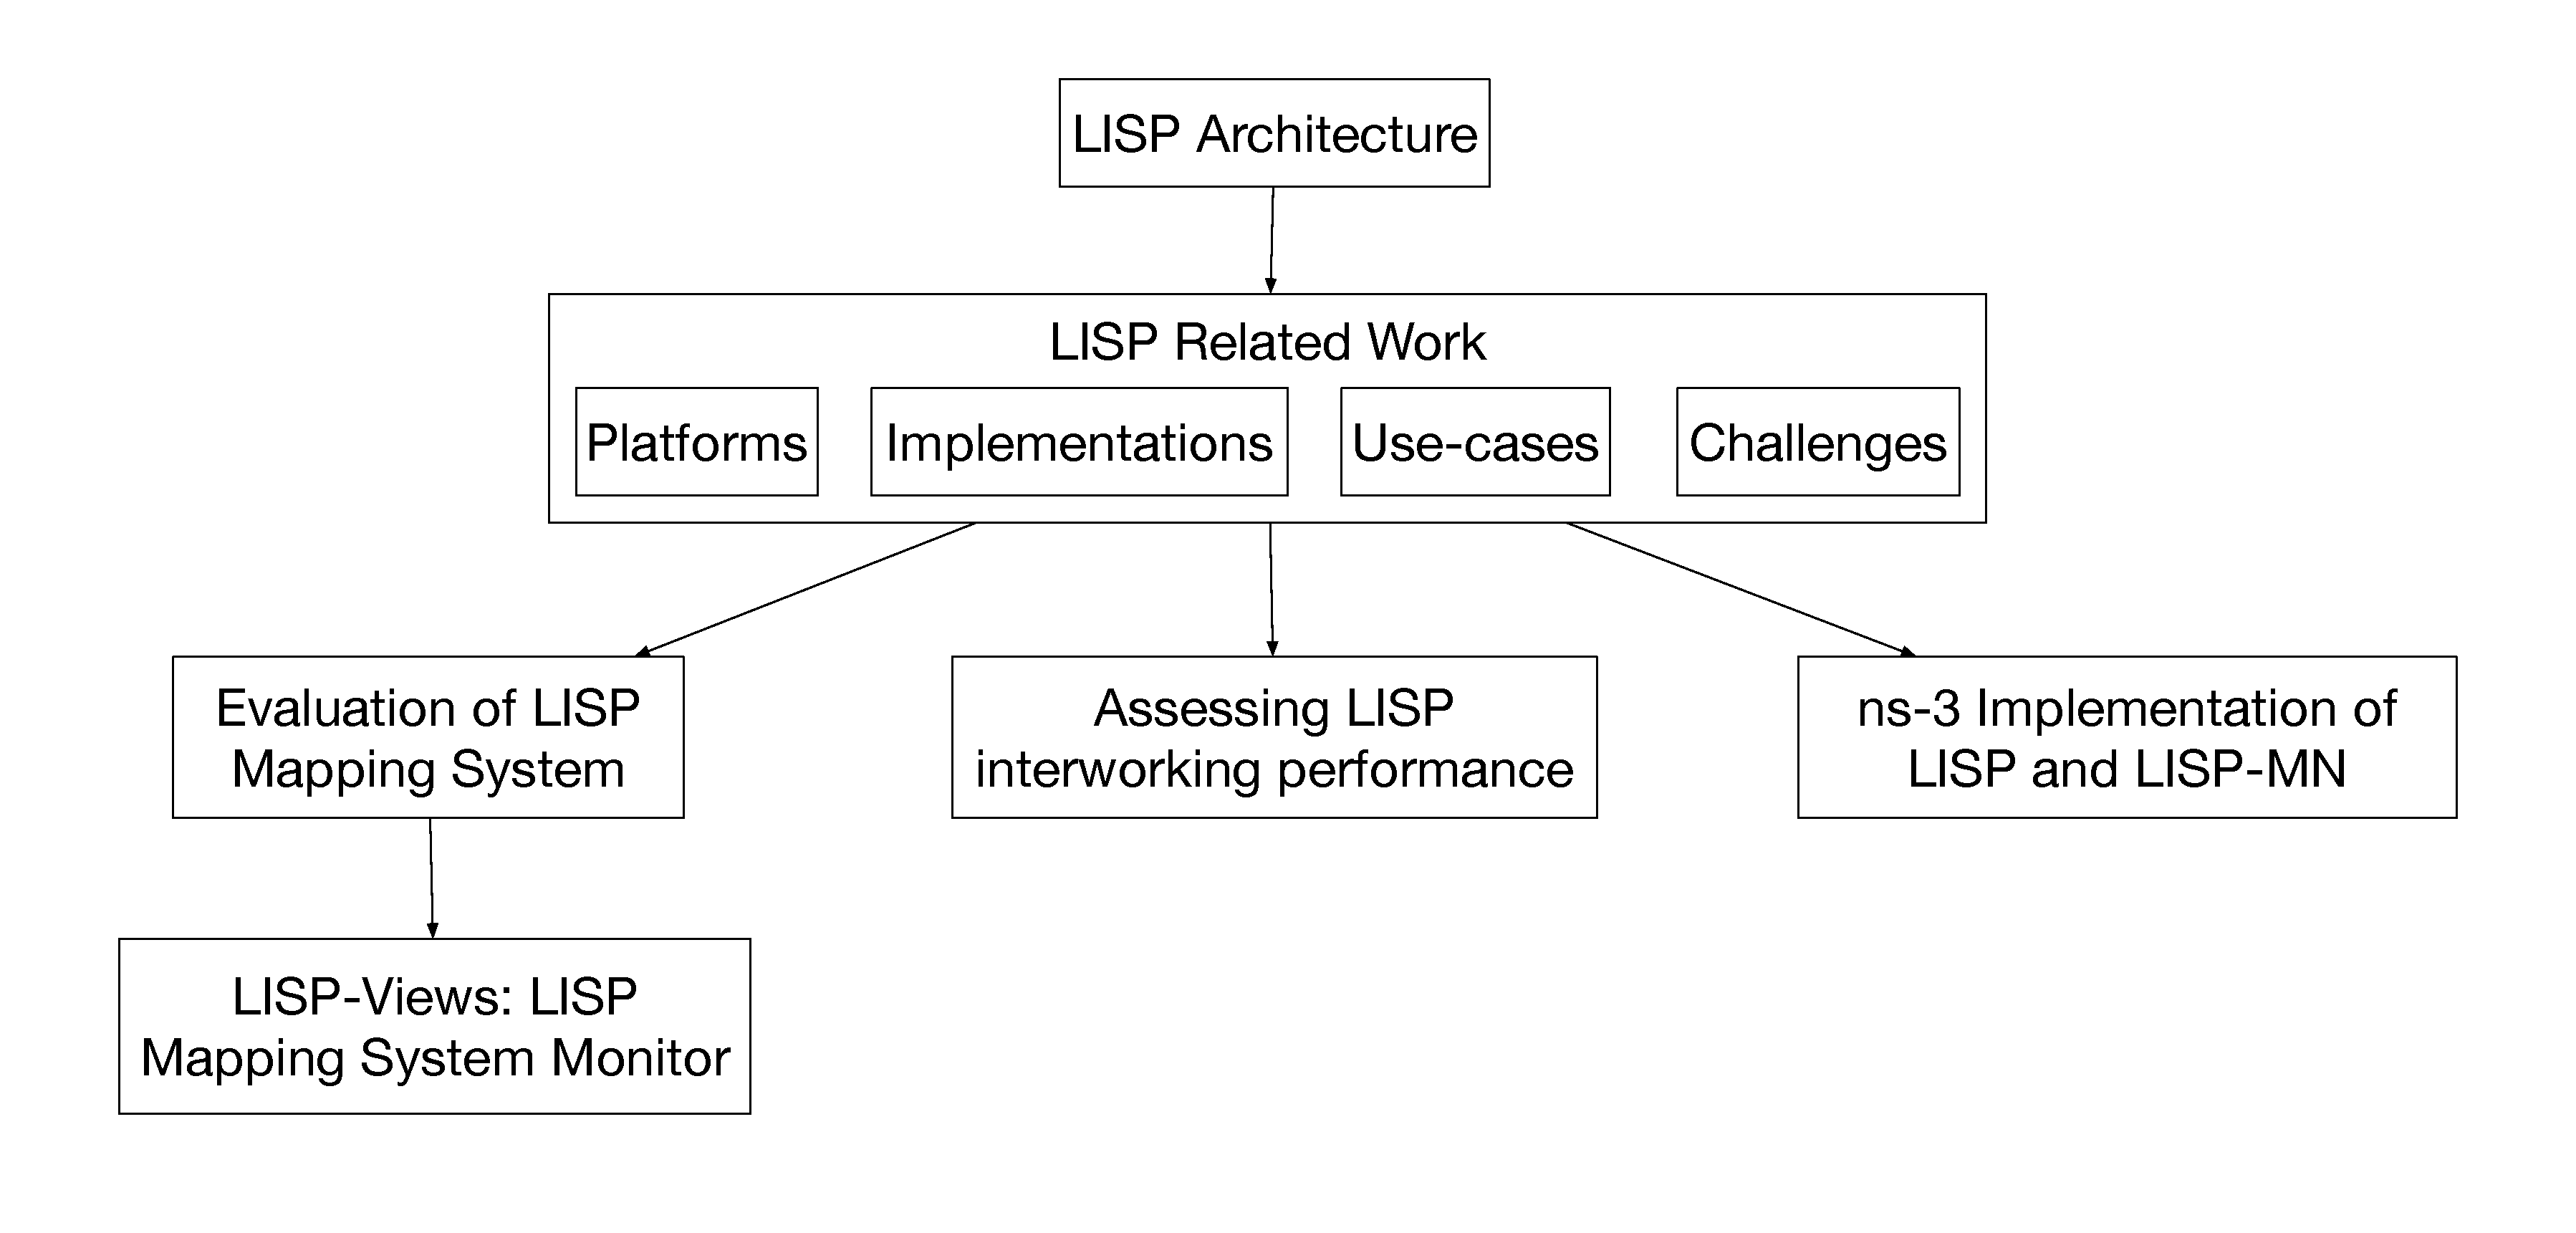
\includegraphics[width=\textwidth]{Pics/structure_thesis.eps}
	\caption{Structure of this dissertation}
	\label{structure_thesis}
\end{figure}
%-< END FIGURE >--------------------------------------------------------------------
The remainder of this dissertation is organized as follows and shown in Fig.~\ref{structure_thesis}:
\begin{itemize}[noitemsep,topsep=0pt]
	\item \emph{Chapter~\ref{cha:lisp_overview}}: Describes the basic LISP knowledge, presenting how the packets are exchanged between two LISP-sites and with the legacy Internet. It also shows the different scenario of LISP mobility.
	\item \emph{Chapter~\ref{cha:related_work}}: The challenges brought by LISP, LISP related studies and missing works are also illustrated. Introduces the LISP current status, such as: the available LISP platforms, the first LISP monitor, the LISP manual management tool, the open source LISP implementations and LISP use-cases.
    \item \emph{Chapter~\ref{cha:mds_evaluation}}: This chapter is about the evaluation of LISP Mapping System. In this chapter, we observe that if the mapping system always provides the same mapping information over time, and if we can obtain the identical mapping answers from the different network entities.
    \item \emph{Chapter~\ref{cha:LISPViews}}: Describes the proposition of LISP-Views: a LISP Mapping System Monitor at large scale. In this chapter, we introduce how this architecture is implemented, how to validate it and what experimental results it can provide.
    \item \emph{Chapter~\ref{cha:pxtr}}: Assesses LISP interworking performance through RIPE Atlas. This chapter presents how the experiments are conducted, how much is the stretch introduced by proxy in the real world, does this stretch have a big impact on the performance or it can be ignored.
    \item \emph{Chapter~\ref{cha:ns-3}}: Introduces ns-3 Implementation of LISP mobility extension and numerically analyses the performance of different LISP mobility scenarios. In this chapter, we first describe how to implement the LISP mobility extension on the ns-3. Then we define three different LISP mobility scenarios, provide the numerical analysis of each scenario, and compare the advantages and shortcomings between them. 
    \item \emph{Chapter~\ref{cha:conclusion}}: Concludes the dissertation and discusses perspectives for further work.
\end{itemize} % Intro
%*******************************************************************************
%****************************** Second Chapter *********************************
%*******************************************************************************

\chapter{LISP Overview}
\label{cha:lisp_overview}

% **************************** Define Graphics Path **************************
\ifpdf
    \graphicspath{{Chapter2/Pics/Raster/}{Chapter2/Pics/PDF/}{Chapter2/}}
\else
    \graphicspath{{Chapter2/Pics/Vector/}{Chapter2/}}
\fi

In this Chapter, the LISP principles and its mechanisms to which we refer to in the reminder of the dissertation are introduced. The basic architecture of LISP is introduced by presenting its Data Plane and Control Plane. We detail how the traffic between two LISP-sites is exchanged by using an example.
A new network element, which is used to allow communication between LISP-site and the legacy Internet, is also presented, as well as the sequence of packets exchange between them. Then, two mechanisms used to update the LISP mapping cache are illustrated. Finally, this chapter ends with the explanation of LISP mobile node, i.e., a LISP-enabled mobile terminal, and the introduction about how the LISP operations are performed when the LISP-enabled node is behind a LISP-speaking router.

% This chapter gives an overview about LISP. Sec.~\ref{sec:background_lisp} presents the basic architecture of LISP, which is composed by Data plane and Control Plane. Sec.~\ref{sec:communication_2_lisp} details how the traffic between two LISP-sites is exchanged. Sec.~\ref{sec:background_Interworking} talks about the interworking between LISP and legacy Internet. Sec.~\ref{sec:updateMechanisms} introduces the mapping cache update mechanism. Finally, Sec.~\ref{sec:lispMN} presents the LISP mobile node.


% %-< SUB SECTION >--------------------------------------------------------------------
% \section{Origin of LISP}
% \label{sec:background_origin}
% State the problem of current Internet routing. Scalability issue etc.


%-< SUB SECTION >--------------------------------------------------------------------
\section{LISP Architecture}
\label{sec:background_lisp}
% \begin{itemize}[noitemsep,topsep=0pt]
%     \item Definition of EID and RLOC.
%     \item Brief introduction of Data Plane and Control Plane.
%     % \item What a mapping looks like: an EID prefix and a list of RLOCs, priority, weight, state.
% \end{itemize}

The \emph{\acrfull{lisp}} separates the traditional IP address role into two logical sub-spaces:
\begin{inparaenum}[(i)]
	\item \emph{\acrfull{eid}} and
	\item \emph{\acrfull{rloc}}.
\end{inparaenum}
Both of them are the conventional IPv4 (32-bit)~\cite{rfc07911981internet} or IPv6 (128-bit)~\cite{deering1998rfc} addresses. The \acrshort{eid} is the identifier of hosts, which is locally routable in the LISP-site. Normally they are the addresses of source and destination hosts. Within the same LISP-site, the hosts can directly communicate with each other via EIDs as in a legacy IP network. The host gets a destination EID in the same way it obtains the destination IP address today, for instance through a \acrfull{dns}~\cite{mockapetrisrfc} lookup or \acrfull{sip}~\cite{rosenbergsip}. RLOCs denote the attachment points of EIDs in the Internet topology, i.e., the source/destination address of the edge routers, behind whom the EIDs can be found. RLOCs addresses are used to forward the packets in the core Internet. 

When packets are transferred between two different LISP-sites, an encapsulation on the edge router is needed: the source and remote destination EIDs are in the inner packet header, while the source and destination RLOCs are in the outer header. % By consequence, the BGP routing tables just announce the RLOCs instead of EIDs so to reduce their table size. 
The EID-prefixes are not necessary to be announced on the Internet core, so the BGP routing table size can be reduced. Similarly, in stub networks, it is not necessary to know the routing information of core Internet any more. The aforementioned encapsulation and forwarding operations are the responsibilities of LISP Data Plane. More details are introduced in Sec.~\ref{sec:data_plane}. To bind the EIDs and RLOCs, a new network entity named \acrfull{mds} is used, whose front end is consisting of Map Resolver (MR) and Map Server (MS)~\cite{rfc6833}. The MDS is not only able to provide the mapping information between the EIDs and RLOCs for the LISP-sites (we simply call them LISP Map-Replies), but also indicate which addresses are not LISP sites and have no RLOCs, meaning that are part of the legacy Internet (these are called Negative Map-Replies). The Control Plane is described in Sec.~\ref{sec:control_plane}.


\subsection{LISP Data Plane}
\label{sec:data_plane}
% \begin{itemize}[noitemsep,topsep=0pt]
%     \item What is ITR and ETR.
%     \item Encapsulate/dencapsulate the packets.
%     \item Forwarding the packets.
%     \item Describe the LISP mapping database.
%     \item LISP cache stored on ITR.
% \end{itemize}
The LISP Data plane mainly takes care of the encapsulation and decapsulation operations done at the source and destination networks. LISP basically provides a level of indirection through a tunneling mechanism over the core Internet (the so called \emph{Default-Free Zone} -- DFZ), in order to provide end-to-end communication. More specifically, any host willing to communicate with another host residing at remote LISP-site, uses its own EID as source address and the EID of other host as destination address to generate regular IP packets. These packets are first transferred as usual to the border router, called \emph{\acrfull{itr}}. \acrshort{itr} performs a mapping lookup in its Cache, or in case of miss, it queries the MDS for the mapping information. Then the \acrshort{itr} encapsulates the regular IP packets into a LISP packet by adding a tunnel header~\cite{rfc6830}, where the RLOC of the \acrshort{itr} is used as source address and the destination RLOC as destination address. After encapsulation, the LISP packets are forwarded over the core Internet. When arriving at the destination border router, called \emph{\acrfull{etr}}, the LISP packets are decapsulated (i.e., the tunnel header is removed) and transferred to the destination host. A device which acts as both an \acrshort{itr} and an \acrshort{etr} is denoted as \emph{\acrshort{xtr}}.

Mappings are stored in two data structures on the \acrshort{xtr}s: the \emph{LISP Database} and the \emph{LISP Cache}. The LISP Database is populated by configuration and stores all known EID-to-RLOC mappings, for which the EID-Prefixes are behind the \acrshort{xtr}. On an \acrshort{itr}, this helps select a source RLOC used in encapsulation. While on an \acrshort{etr}, it allows to verify whether itself is the proper \acrshort{etr} connecting to the destination EID, so that such \acrshort{etr} is able to forward the decapsulated packets to the final destination. 

The LISP Cache temporally stores mappings for the EID-prefixes of the remote communicating end-points. On an \acrshort{itr}, it is used to select the destination RLOC of the outer header of the LISP-encapsulated packet. While on an \acrshort{etr}, it is used to perform a basic anti-spoof verification. Different from the LISP Database, the LISP Cache is populated on demand. The procedure is triggered by the first packet of a new flow, which can not find a suitable mapping for the destination EID among the mappings stored in the LISP Cache. The mappings in the LISP Cache are purged if not used upon expiration of a timeout~(\cite{lispCacheCost,lispCacheDive,lispCacheLRU,lispCacheModel}).

\subsection{LISP Control Plane}
\label{sec:control_plane}
% \begin{itemize}[noitemsep,topsep=0pt]
%     % \item LISP mapping system.
%     \item Map-Register and Map-Notify.
%     \item Map-Request and Map-Reply (3 types: LISP Map-Reply, Negative Map-Reply, and No Map-Reply).
%     % \item What a mapping looks like: an EID prefix and a list of RLOCs, priority, weight, state.
% \end{itemize}

The LISP Control plane is mainly tasked to discover the associations of EIDs with RLOCs, i.e., find the \emph{mappings}. A new network entity named \emph{\acrfull{mds}} is introduced by LISP to perform such EID-to-RLOC distribution. In particular, a mapping contains an EID prefix and an associated list of RLOC tuples: \emph{$<$RLOC, Priority, Weight$>$}. The RLOC refers to the IP address of each \acrshort{xtr} interface. Each RLOC is assigned a Priority. The RLOC with the highest priority is preferred. % There are 8 bits reserved to indicate the priority, where the highest priority is presented by the lowest value in the LISP implementation. A value of 255 means that this RLOC must not be used for forwarding. 
The weight is taken into account only to perform load balancing in the case of several RLOCs having the same priority. % Weight is encoded as a relative weight of total packets that match the mapping entry.

%-< FIGURE >--------------------------------------------------------------------
\begin{figure}[!t]
	\centering
	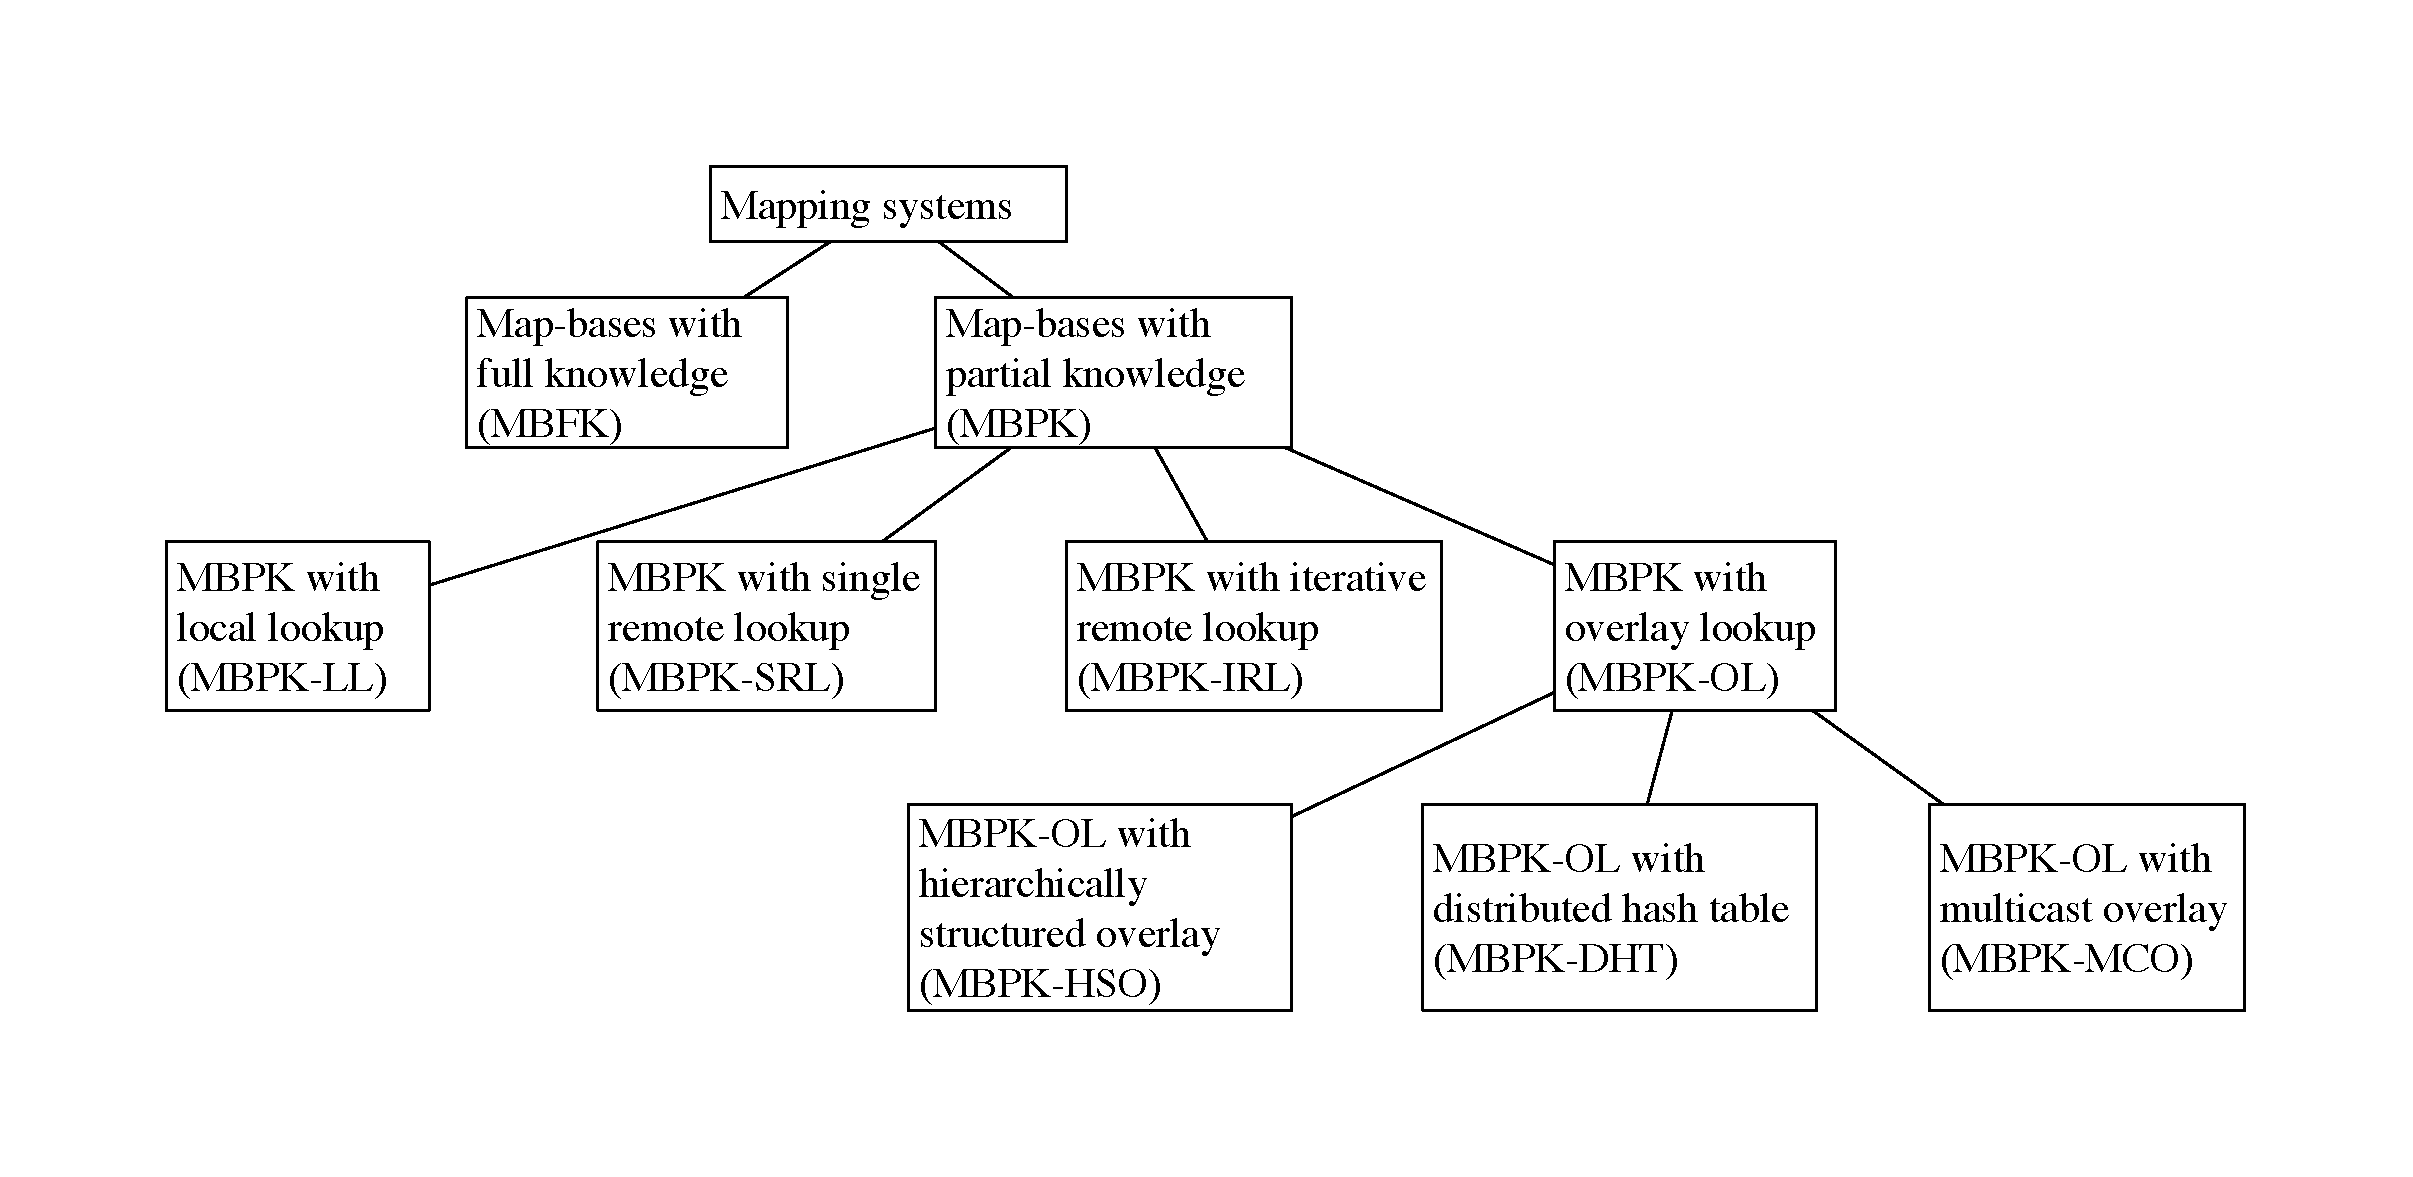
\includegraphics[width=\textwidth]{Pics/Hierarchical_taxonomy_of_mapping_systems.eps}
	\caption{Hierarchical taxonomy of mapping systems (from \cite{info3-articles-2013-06})}
	\label{Hierarchical_taxonomy_of_mapping_systems}
\end{figure}
%-< END FIGURE >--------------------------------------------------------------------
The current BGP-based Internet routing architecture relies on a push model, in which routing information is pushed to the whole Internet. The Locator/Identifier Split-based Internet routing instead relies on a pull model, where the \emph{\acrfull{mds}} provides a mapping upon an explicit query,\footnote{The terms \emph{\acrfull{mds}} and \emph{mapping system} are used interchangeably in this dissertation.}  where routing information is pulled only when actually needed. This paradigm shift requires making routing information available in an on-demand manner. % To achieve this purpose, a new system called \emph{Mapping System} is introduced.
Fig.~\ref{Hierarchical_taxonomy_of_mapping_systems} shows the current possible taxonomy of mapping systems~\cite{info3-articles-2013-06}. So far, several mapping systems have been proposed for LISP, such as: LISP-TREE~\cite{lispTree}, LISP-NERD (Not-so-novel EID to RLOC Database)~\cite{lear2013nerd} and LISP-CONS (Content distribution Overlay Network Service for LISP)~\cite{brim2008lisp}. However, only two have been deployed: \emph{LISP Alternative Logical Topology (LISP+ALT)}~\cite{rfc6836} and \emph{LISP Delegated Database Tree (LISP-DDT)}~\cite{lispDDT}.


\subsubsection{LISP+ALT}
\label{sec:lispalt}
%-< FIGURE >--------------------------------------------------------------------
\begin{figure}[!t]
	\centering
	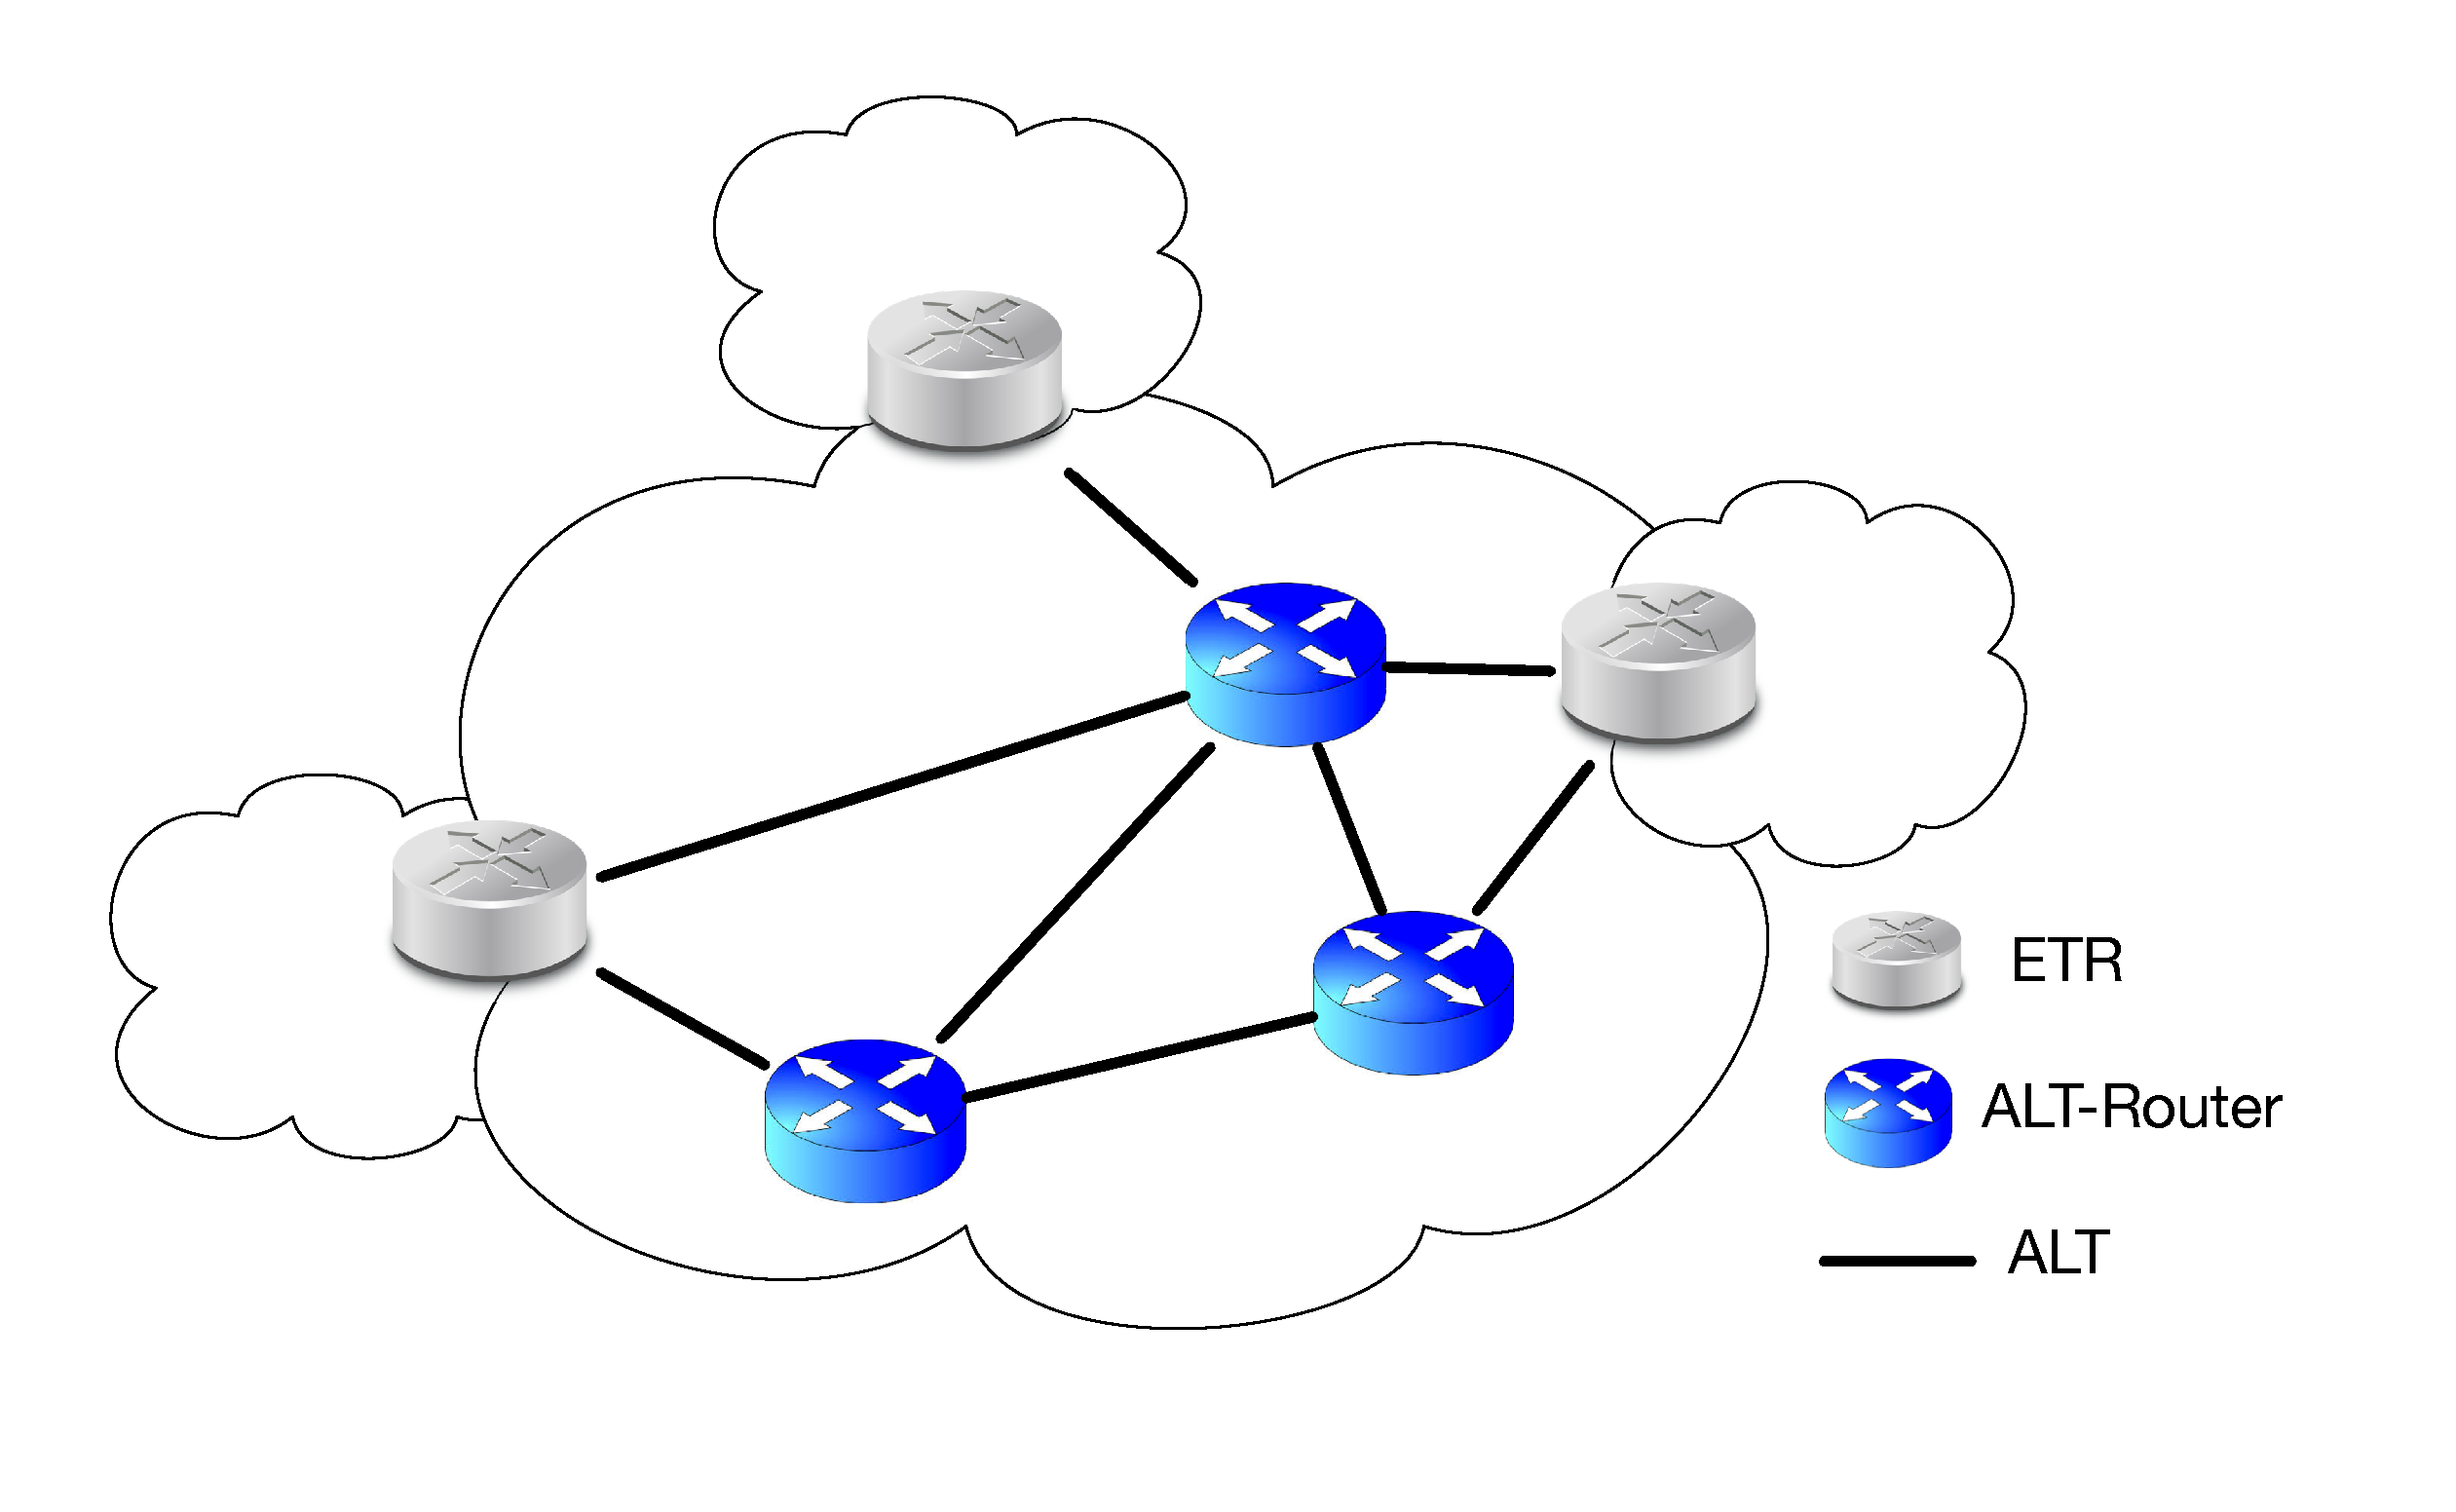
\includegraphics[width=0.9\textwidth]{Chapter2/Pics/LISP_ALT.eps}
	\caption{Illustration of the LISP+ALT topology}
	\label{LISP_ALT}
\end{figure}
%-< END FIGURE >--------------------------------------------------------------------
\emph{LISP+ALT} was the initial mapping system for LISP, where the \acrshort{etr}s store mappings they are authoritative for~\cite{lispCCR}. The basic idea is to use BGP to construct an overlay, named Alternative Logical Topology (ALT), to establish reachability between \acrshort{etr}s via tunnels (e.g., GRE tunnels~\cite{farinacci2000rfc}). As shown in Fig.~\ref{LISP_ALT}, the routers in the ALT are called ALT-Routers. Each ALT–Router maintains a BGP session with its neighbor and announces the EID–prefixes it is authoritative for. These EIDs are then routable in the ALT. Note that the ALT–Routers only exchange aggregated EID-prefixes that can be reached through them between neighbors, but they do not contain the mapping information. To get a mapping, an \acrshort{itr} constructs a Map-Request for the queried EID by using its own RLOC as source address and the queried EID as destination address, then sends it to an ALT-Router. The Map-Request is forwarded over the ALT and eventually reaches an originator \acrshort{etr} for the EID-prefix that matches the destination EID. This \acrshort{etr} resolves the Map-Request and directly sends back a Map-Reply to the inquirer \acrshort{itr}, this time not using the ALT. LISP-ALT belongs to the Map-Bases with Partial Knowledge using Hierarchically Structured Overlay (MBPK-HSO) in Fig.~\ref{Hierarchical_taxonomy_of_mapping_systems}.


\subsubsection{LISP-DDT}
\label{sec:lispddt}
%-< FIGURE >--------------------------------------------------------------------
\begin{figure}[!t]
	\centering
	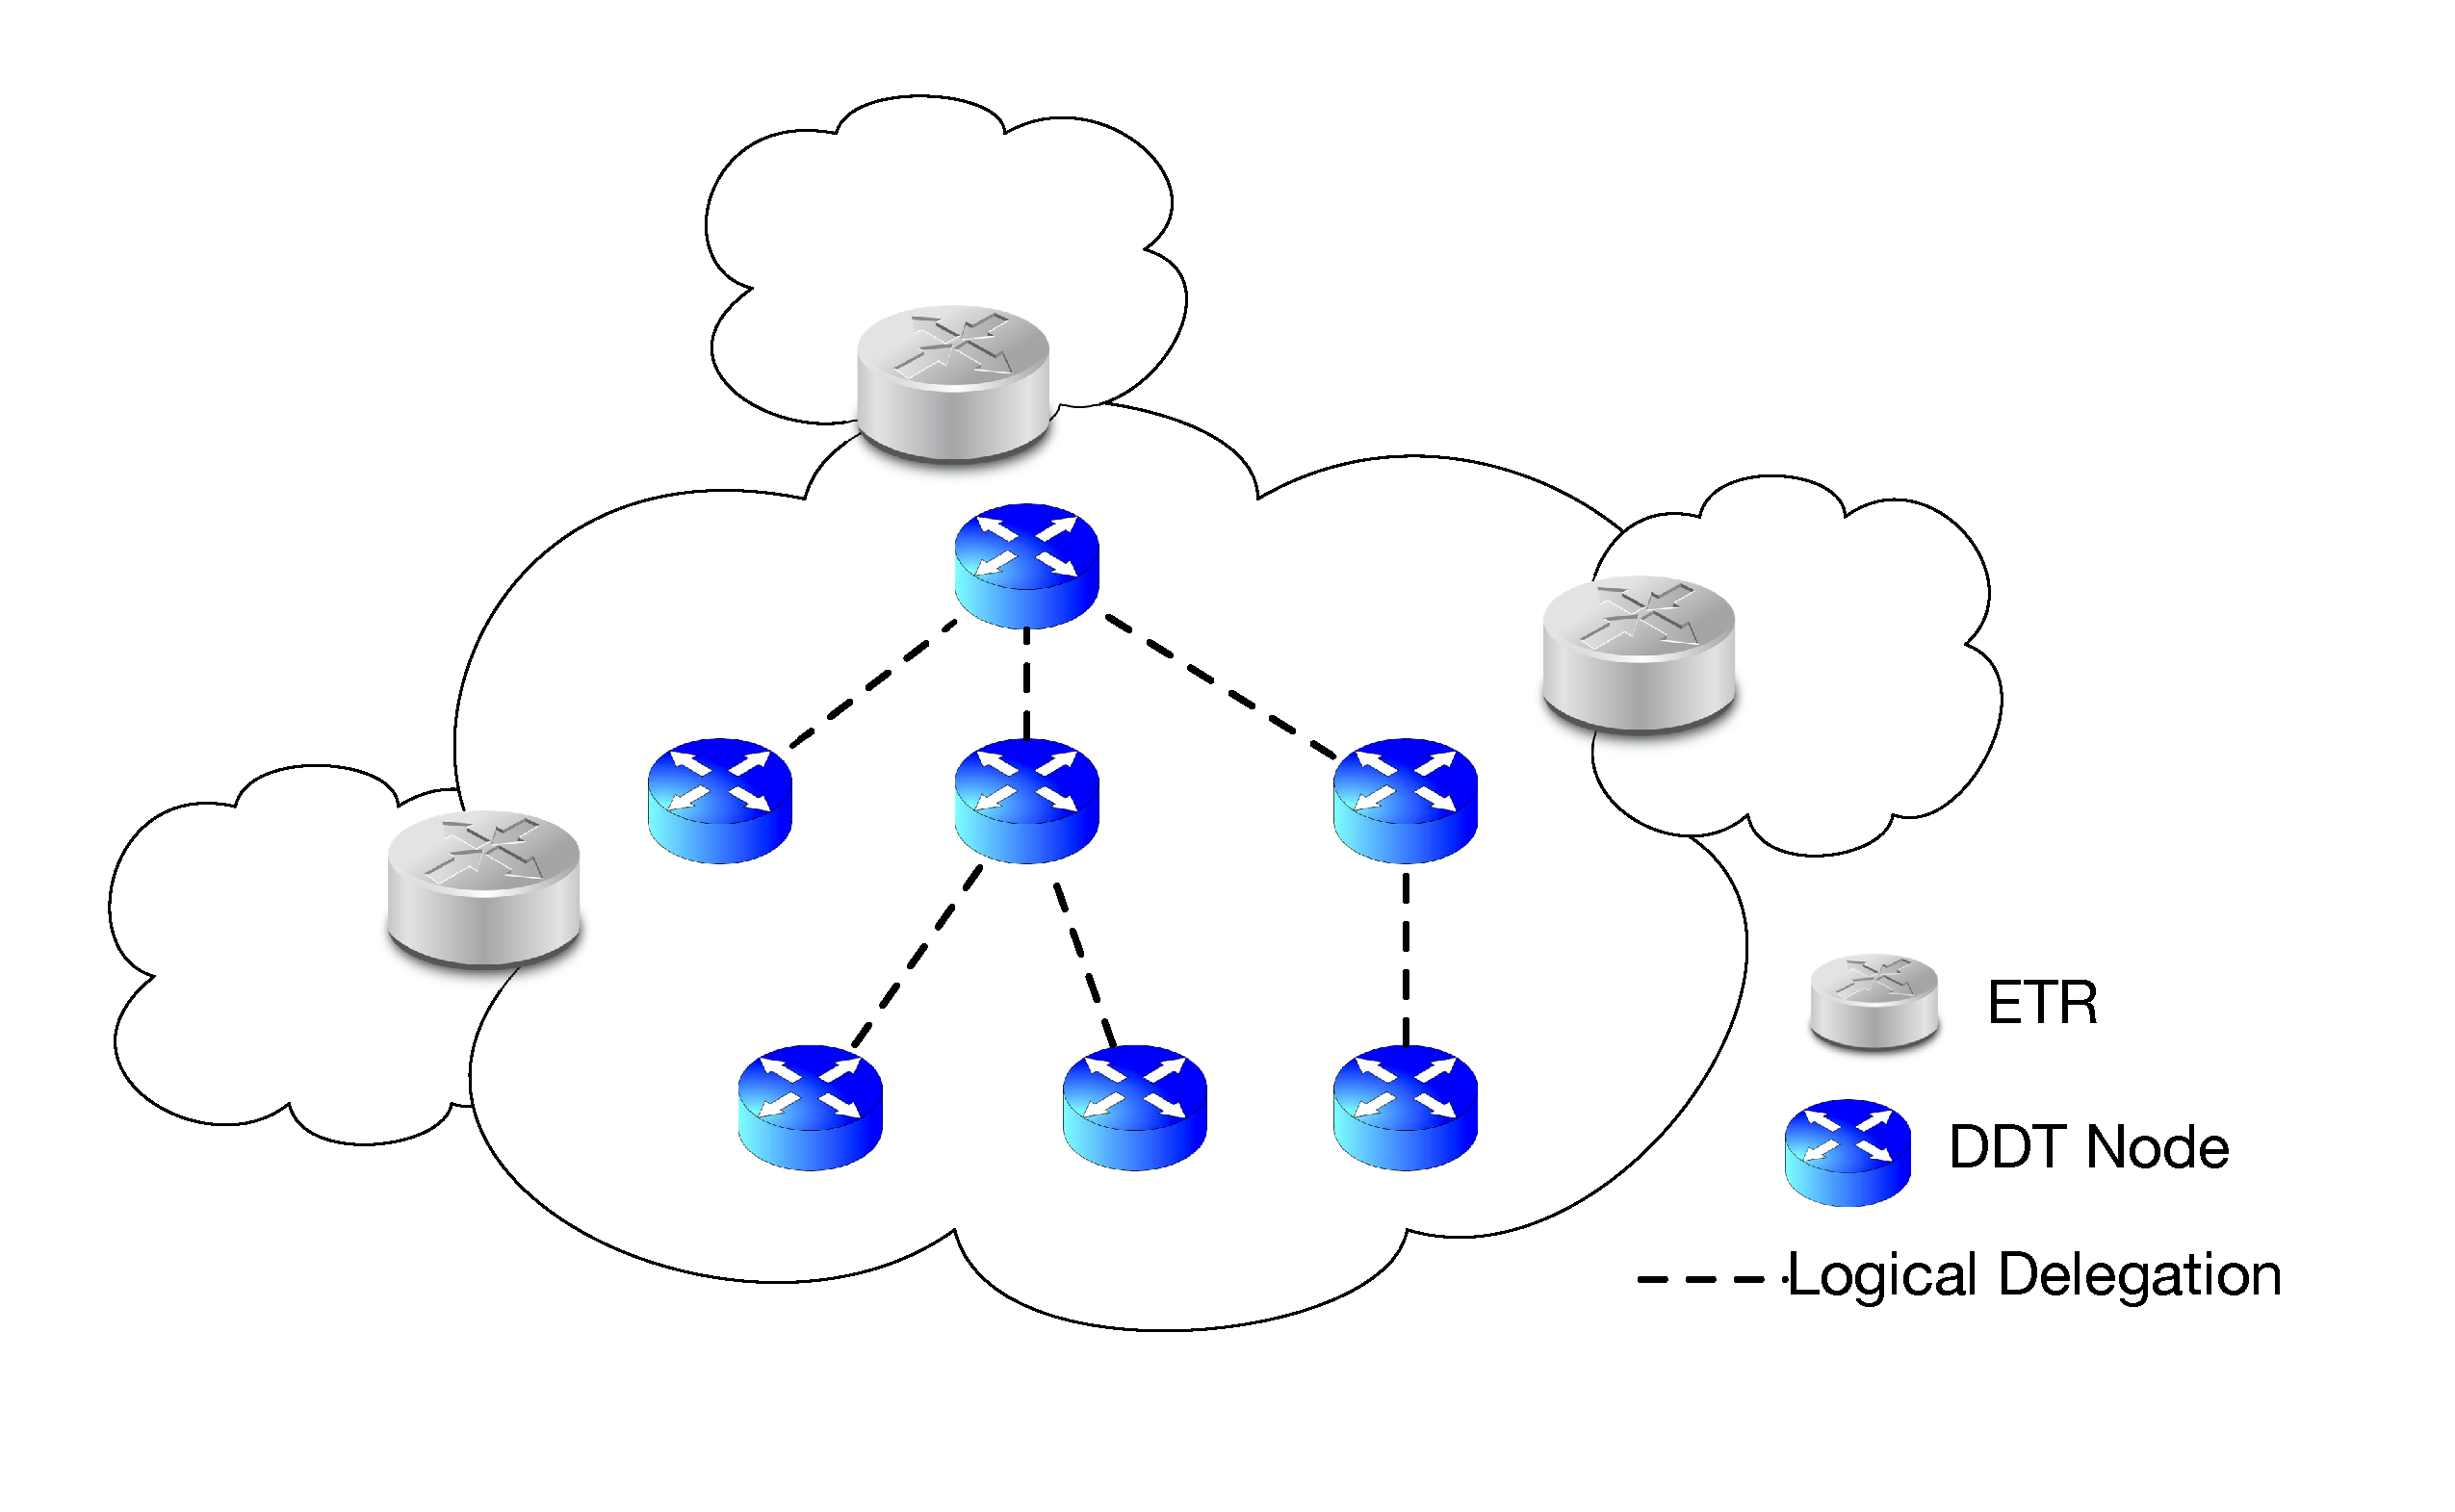
\includegraphics[width=0.9\textwidth]{Chapter2/Pics/LISP_DDT.eps}
	\caption{Illustration of the LISP-DDT topology}
	\label{LISP_DDT}
\end{figure}
%-< END FIGURE >--------------------------------------------------------------------
\emph{LISP-DDT} is a hierarchical distributed database that embodies the delegation of authority to provide mappings from LISP EIDs to RLOCs . Its hierarchical organization is shown in Fig.~\ref{LISP_DDT}. It consists of \emph{Map-Resolvers (MRs)} and \emph{Map-Servers (MSes)} to provide a simplified "front end". The MR is a network infrastructure component that accepts LISP Encapsulated Map-Requests from an \acrshort{itr} and resolves the mapping using a DNS-like distributed database. The MS learns of EID-Prefix mapping entries (a list of EID-Prefixes plus a set of RLOC tuples) from \acrshort{etr}s. The hierarchy is maintained as a tree where a root server is responsible for the entire EID space. This space is divided into several portions and each one is managed by one of the root’s children.
% where each node is responsible for a specific part of the EID-prefixes. A child node is responsible for a portion of the EID-prefixes of its parent. 
Mapping information is only stored at the tree leaves, which are made of MSes. Intermediate nodes only maintain pointers to their children.

If an \acrshort{itr} cannot find a mapping in its LISP Cache for a new flow, it sends a query, called \emph{Map-Request}, to a \acrshort{mr}~\cite{rfc6833}. The \acrshort{mr} determines whether the queried destination IP address is an EID. If not, a \emph{Negative Map-Reply} is directly returned; otherwise, the root server is queried. The root replies with a pointer to its child node responsible for the queried EID. The process is recursively repeated to find the child root of the sub-tree where a mapping can be retrieved for the queried EID. When the leaf is reached, the mapping is then retrieved by sending a Map-Request to the \acrshort{etr} authoritative for the matching EID-prefix. The \acrshort{etr} in turn directly replies a \emph{Map-Reply} message containing the whole requested mapping information to the \acrshort{itr} initiating the query.

When an \acrshort{etr} first contacts an \acrshort{ms} after restarting or changing its database, it sends the Map-Register messages to the \acrshort{ms} to publish its EID-prefixes as well as the mapping information. % at an increased frequency, up to one every 20 seconds. 
For maintaining the association, the registration interval should be expanded to at least 1 minute. If the MS has not received a valid Map-Register within the past 3 minutes, it removes the registration of this \acrshort{etr}. If the "want-map-notify" (M-bit) flag is set in Map-Register, the received MS needs to send back a Map-Notify message to inform the \acrshort{etr} that the Map-Register has been received and processed. If the "proxy Map-Reply" flag (P-bit) is set, the MS answers the Map-Requests to the queried \acrshort{itr} by providing the mapping information on behalf of the \acrshort{etr}. \acrshort{mr}s offer an interface to the \acrshort{mds} for the \acrshort{xtr}s, so that the whole complex \acrshort{mds} mechanism can be hided.


\subsection{Communication between two LISP-sites}
\label{sec:communication_2_lisp}
%-< FIGURE >--------------------------------------------------------------------
\begin{figure}[!t]
	\centering
	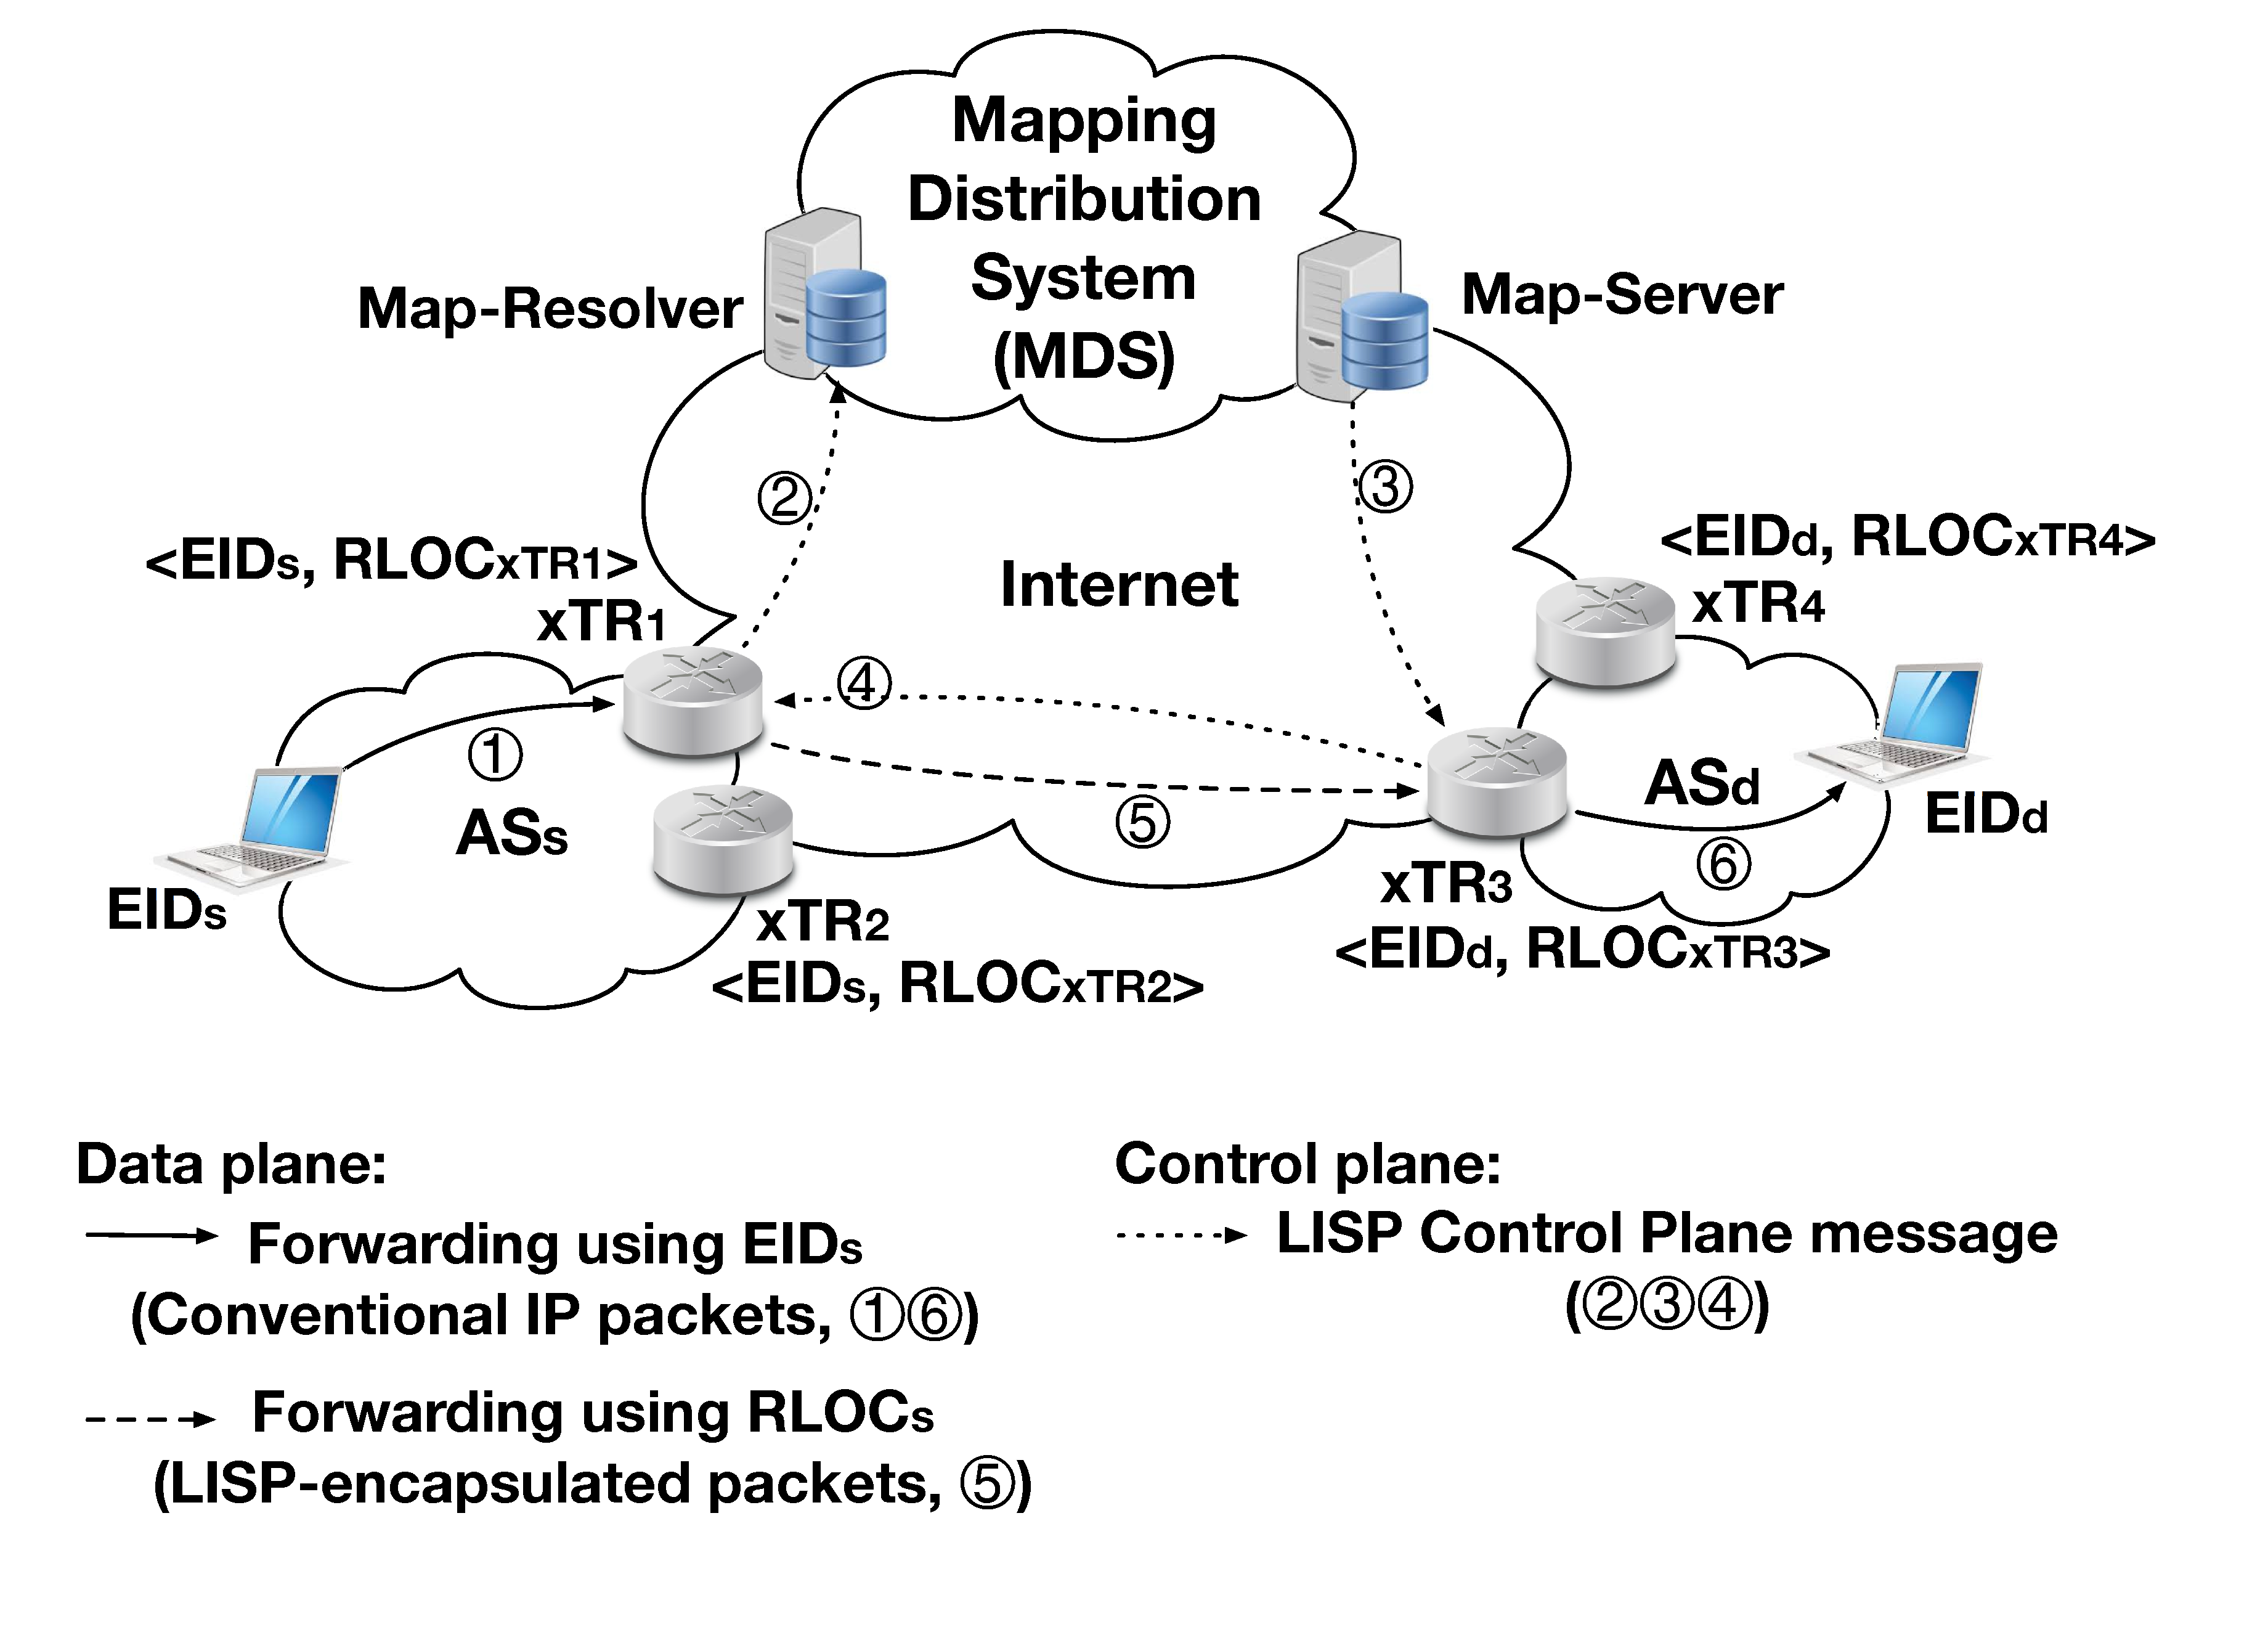
\includegraphics[width=0.9\textwidth]{Pics/LISP_D_C_planes.eps}
	\caption{LISP architecture overview}
	\label{LISP_archi}
\end{figure}
%-< END FIGURE >--------------------------------------------------------------------
We use Fig.~\ref{LISP_archi} as an example to describe how the LISP packets are processed in details in the case of the packets exchange between two LISP-sites.

When the host in the $AS_s$ communicates with the host in the $AS_d$, it uses $EID_s$ as source address and $EID_d$ as destination address. After the conventional IP routing to $xTR_1$ (the function of \acrshort{itr} and \acrshort{etr} are combined together in Fig.~\ref{LISP_archi}) labeled as \emph{"1"}, $ITR_1$ first checks in its mapping cache~\cite{lispCacheCost} to find out the association between $EID_d$ and its RLOC. If there is no record, it sends a Map-Request to Map-Resolver (MR), labeled as \emph{"2"}. \acrshort{mr} searches which \acrfull{ms} stores the mapping information of $EID_d$ and forwards the Map-Request to that \acrshort{ms}. If \acrshort{ms} is authoritative (i.e., acts as a proxy), it directly returns back a Map-Reply containing the mapping information (this procedure is not labeled in the figure). If not, after forwarding the Map-Request within \acrshort{mds} with the procedure described in Sec.~\ref{sec:lispddt} to \acrshort{ms} and then to the destination side (label \emph{"3"}), $xTR_1$ receives a Map-Reply from one of \acrshort{etr}s of $EID_d$ (label \emph{"4"}). If the Map-Reply shows that the priority of $ETR_3$ is higher than $ETR_4$, then the $ITR_1$ encapsulates the packets by adding $RLOC_{ETR_3}$ as the destination address and $RLOC_{ITR_1}$ as the source address in the outer header and sends the encapsulated packets through the Internet as labeled \emph{"5"} in Fig.~\ref{LISP_archi}. Once $ETR_3$ receives these packets, it decapsulates and forwards them by using the original IP packets (label \emph{"6"}). If the destination site is not a LISP-site, the MR directly returns back the Map-Reply without mapping information to $ITR_1$.

Based on LISP architecture, there are three types of outcomes for a query:
\begin{itemize}[noitemsep,topsep=0pt]
%\begin{inparaenum}[(i)]
	\item \emph{LISP Map-Reply}, means that the queried IP address belongs to a LISP site (i.e., EID) and the Map-Reply contains the mapping information for this site, including: the association between the EID-prefix that queried EID belongs to, and the list of RLOC tuples $<$RLOC, Priority, Weight$>$ of the destination site.
	\item \emph{Negative Map-Reply}, means that the prefix covering the queried IP address belongs to a non-LISP site (i.e., conventional site), and the Map-Reply contains no mapping information. We consider these two kinds of replies as successful queries.
    \item \emph{No Map-Reply}, means that the \acrshort{xtr} does not receive any reply during a certain time. According to the standard described in~\cite{rfc6830}, the time-out is set to 3 seconds. But this value can be modified in the implementation to adapt the experiment needs. In this case, we consider the query as failed.
%\end{inparaenum}
\end{itemize}


%-< SECTION >--------------------------------------------------------------------
\section{Interworking With Legency Internet}
\label{sec:background_Interworking}
% \begin{itemize}[noitemsep,topsep=0pt]
%     \item Describe what is PxTR.
%     \item How it works when a terminal behind LISP-site communicates with a terminal on the legacy Internet.
% \end{itemize}

Sec.~\ref{sec:communication_2_lisp} describes how the LISP packets are exchanged between two LISP-sites. This section discusses how the packets are processed when a terminal behind LISP-site communicates with a terminal on the legacy Internet.

%-< FIGURE >--------------------------------------------------------------------
\begin{figure}[!t]
	\centering
	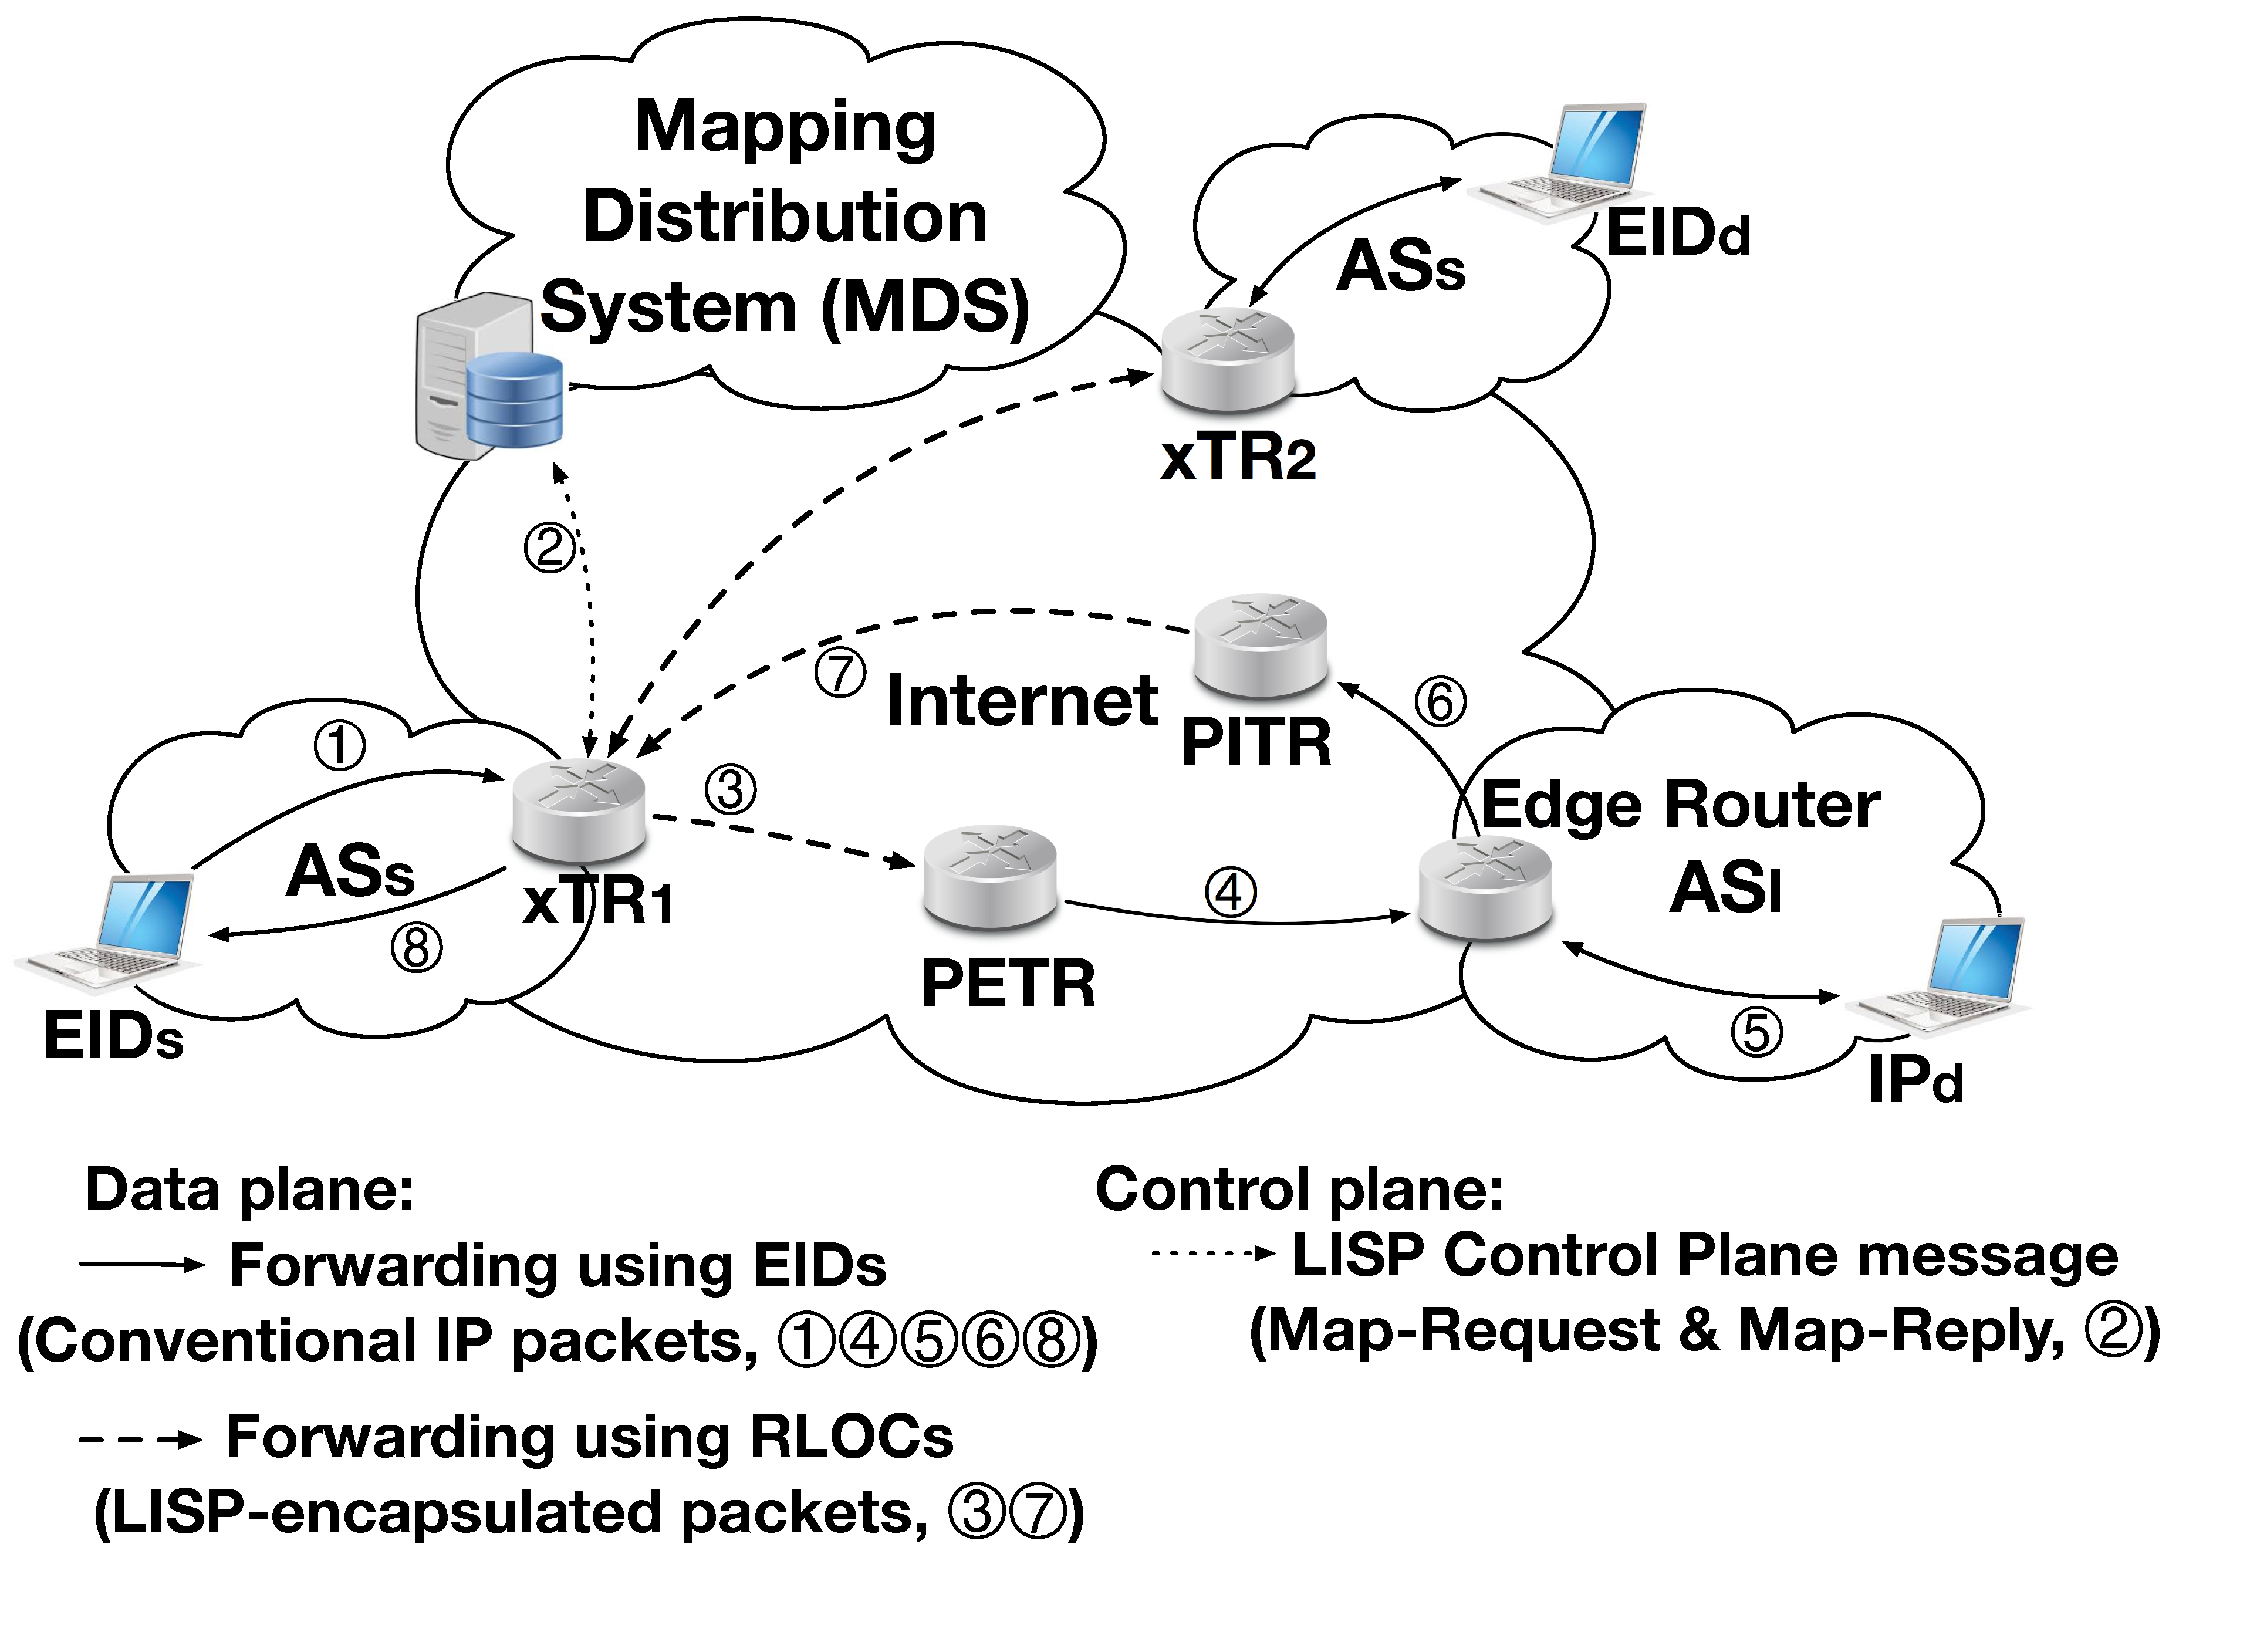
\includegraphics[width=0.9\textwidth]{Pics/LISP_archi_PxTR.eps}
	\caption{LISP architecture with the packets forwarding sequence}
	\label{LISP_archi_PxTR}
\end{figure}
%-< END FIGURE >--------------------------------------------------------------------
Although EIDs are syntactically identical to IPv4 or IPv6 addresses, routes to them are not announced in the global routing system, so an interoperability mechanism is needed for non-LISP-speaking sites to exchange traffic with LISP-speaking sites. Thus, two new network elements are introduced: LISP \acrfull{pitr} and LISP \acrfull{petr}. The \acrshort{pitr} acts as an intermediate LISP \acrshort{itr} for the hosts on legacy Internet. It is in charge of announcing one or more highly aggregated EID-Prefixes on behalf of LISP-sites into the public Internet and receives the traffic from the public Internet to encapsulate them as LISP packets. The \acrshort{petr} acts as an \acrshort{etr} for traffic destined to non-LISP sites. It receives the traffic from the \acrshort{itr}s, decapsulates the LISP packets into conventional IP packets and sends them to the legacy Internet.

Fig.~\ref{LISP_archi_PxTR} shows an example for the packets exchanging between LISP-site and non LISP-site (i.e., legacy Internet). The host with $EID_s$ in the $AS_s$ exchanges the packets with the host with the $IP_d$ in the $AS_l$. With the same procedure introduced in Sec.~\ref{sec:communication_2_lisp} labeled as \emph{"1"} and \emph{"2"} in Fig.~\ref{LISP_archi}, the original IP packets are sent from host to $xTR_1$, and the later one sends the Map-Request to \acrshort{mds} to query the mapping information. Since the destination is in a non-LISP-Site, the MR directly returns back the Map-Reply without mapping information (i.e., Negative Map-Reply) to $xTR_1$, the packet can either be sent non-encapsulated or the $xTR_1$ encapsulates it using the statically configured RLOC of the \acrshort{petr} as the outer destination address and forwards the LISP packets there. When \acrshort{petr} receives the LISP-encapsulated packets, it performs a decapsulation as an \acrshort{etr} and then forwards the inner IP packets to the legacy destination host by using the normal BGP routing, labeled as procedure \emph{"4"} and \emph{"5"} in Fig.~\ref{LISP_archi_PxTR}. 

When the packets come back, they are forwarded in a traditional way from the host with address $IP_d$ in $AS_l$ to the \acrshort{pitr}, denoted as procedure \emph{"5"} and \emph{"6"} in Fig.~\ref{LISP_archi_PxTR}. A \acrshort{pitr} shares many characteristics with \acrshort{itr}s, as it also queries the mapping information of destination to the \acrshort{mds} and encapsulates the non-LISP Internet traffic into LISP-encapsulated packets and route them to their destination RLOCs (label \emph{"7"}). Target $ETR_1$ then dencapsulates the packets and send them to the destination host $EID_s$. The \acrshort{petr} and \acrshort{pitr} can be noted together as \acrshort{pxtr} if they are located on a same physical router.



%-< SECTION >--------------------------------------------------------------------
\section{Mapping Cache Update Mechanisms}
\label{sec:updateMechanisms}
% When the \acrshort{etr}s change their mappings, the only way that remote \acrshort{itr} can get the updated mapping information is to re-request the mapping. Thus, two protocol approaches are proposed to get the latest mapping. They are Solicit-Map-Request and Map-Versioning.
Given that LISP mapping distribution is based on a pull model, in case that mapping changes occur in \acrshort{etr}s, the only way that makes remote \acrshort{itr}s be aware of such change and update the corresponding mapping information is to request again the mappings to \acrshort{etr}s. Thus, two mechanisms are proposed to notify \acrshort{itr}s that mapping has changed and they need to get the latest mapping: Solicit-Map-Request and Map-Versionning.


%-< SUB SECTION >--------------------------------------------------------------------
\subsection{Solicit-Map-Request (SMR)}
\label{sec:SMR}
Soliciting a Map-Request is used by \acrshort{etr}s to tell remote \acrshort{itr}s to update the mappings they have cached. When the mappings in the Database of an \acrshort{etr} changes, the \acrshort{etr} sends the Map-Requests with the \acrshort{smr} bit set (called \acrfull{smr} message) for each RLOC in its Cache. A remote \acrshort{itr} that receives the \acrshort{smr} message will take a check in its Cache whether the source RLOC of the \acrshort{smr} message, i.e., the RLOC of \acrshort{etr} with mappings change is in its Cache. If yes, the remote \acrshort{itr} sends a Map-Request to the MR (as shown in the left hand part of Fig.~\ref{SMR_schema}) or directly to the sender of \acrshort{smr} (as shown in the right hand part of Fig.~\ref{SMR_schema}). % In the case that the sender of \acrshort{smr} has the unique RLOC in the Locator-set of \acrshort{etr} that \acrshort{itr} caches, the \acrshort{itr} can only send the Map-Request to the MR, to avoid the \acrshort{etr} changes its RLOC and can not receive the SMR-invoked Map-Request any more. 
If the RLOC\yue{check} of sender is not in the Cache of \acrshort{itr} any longer, the later drops the \acrshort{smr} and does not send the Map-Request. The later situation occurs when the \acrshort{etr} sends the \acrshort{smr} to all RLOCs stored in its Cache, but the remote \acrshort{itr} actually has not sent the packets to it for a long time. Between sending the \acrshort{smr} message and receiving the new Map-Reply, the \acrshort{itr} continues to use the mapping information previously cached, and that may cause packet loss.
%-< FIGURE >--------------------------------------------------------------------
\begin{figure}[!t]
	\centering
	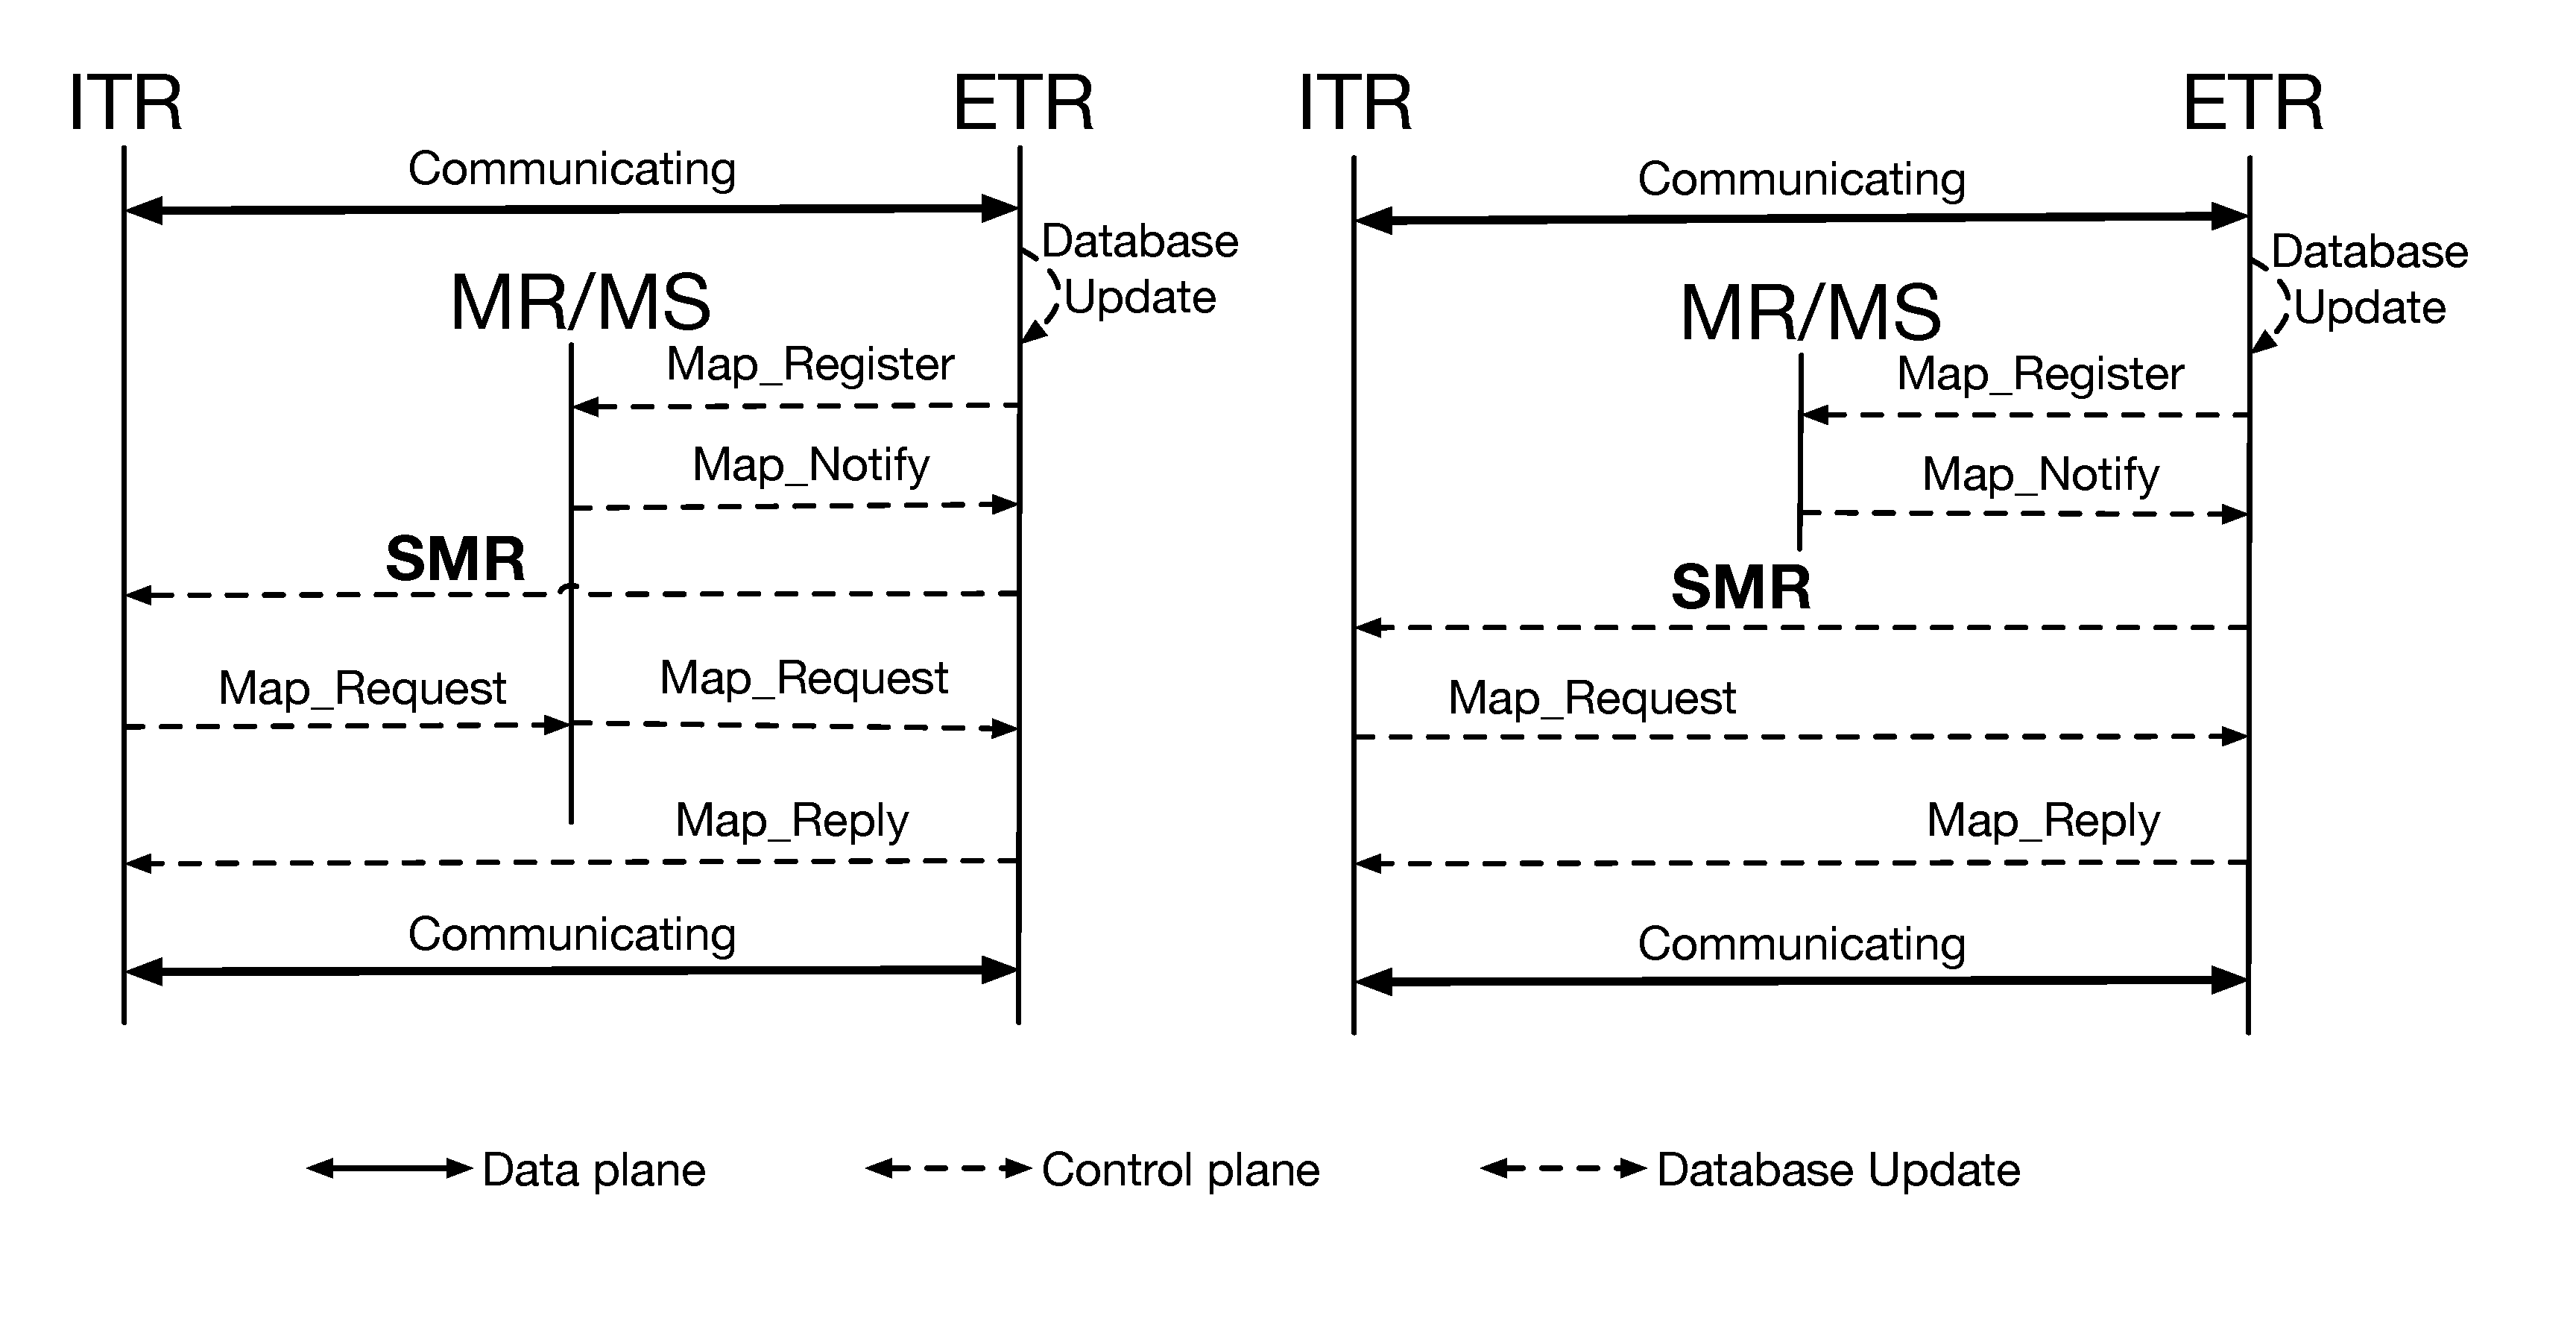
\includegraphics[width=\textwidth]{Pics/SMR_schema.eps}
	\caption{Packet sequence of LISP SMR mechanism}
	\label{SMR_schema}
\end{figure}
%-< END FIGURE >--------------------------------------------------------------------


%-< SUB SECTION >--------------------------------------------------------------------
\subsection{Map-Versioning}
\label{sec:MapVersionning}
%-< FIGURE >--------------------------------------------------------------------
\begin{figure}[!t]
	\centering
	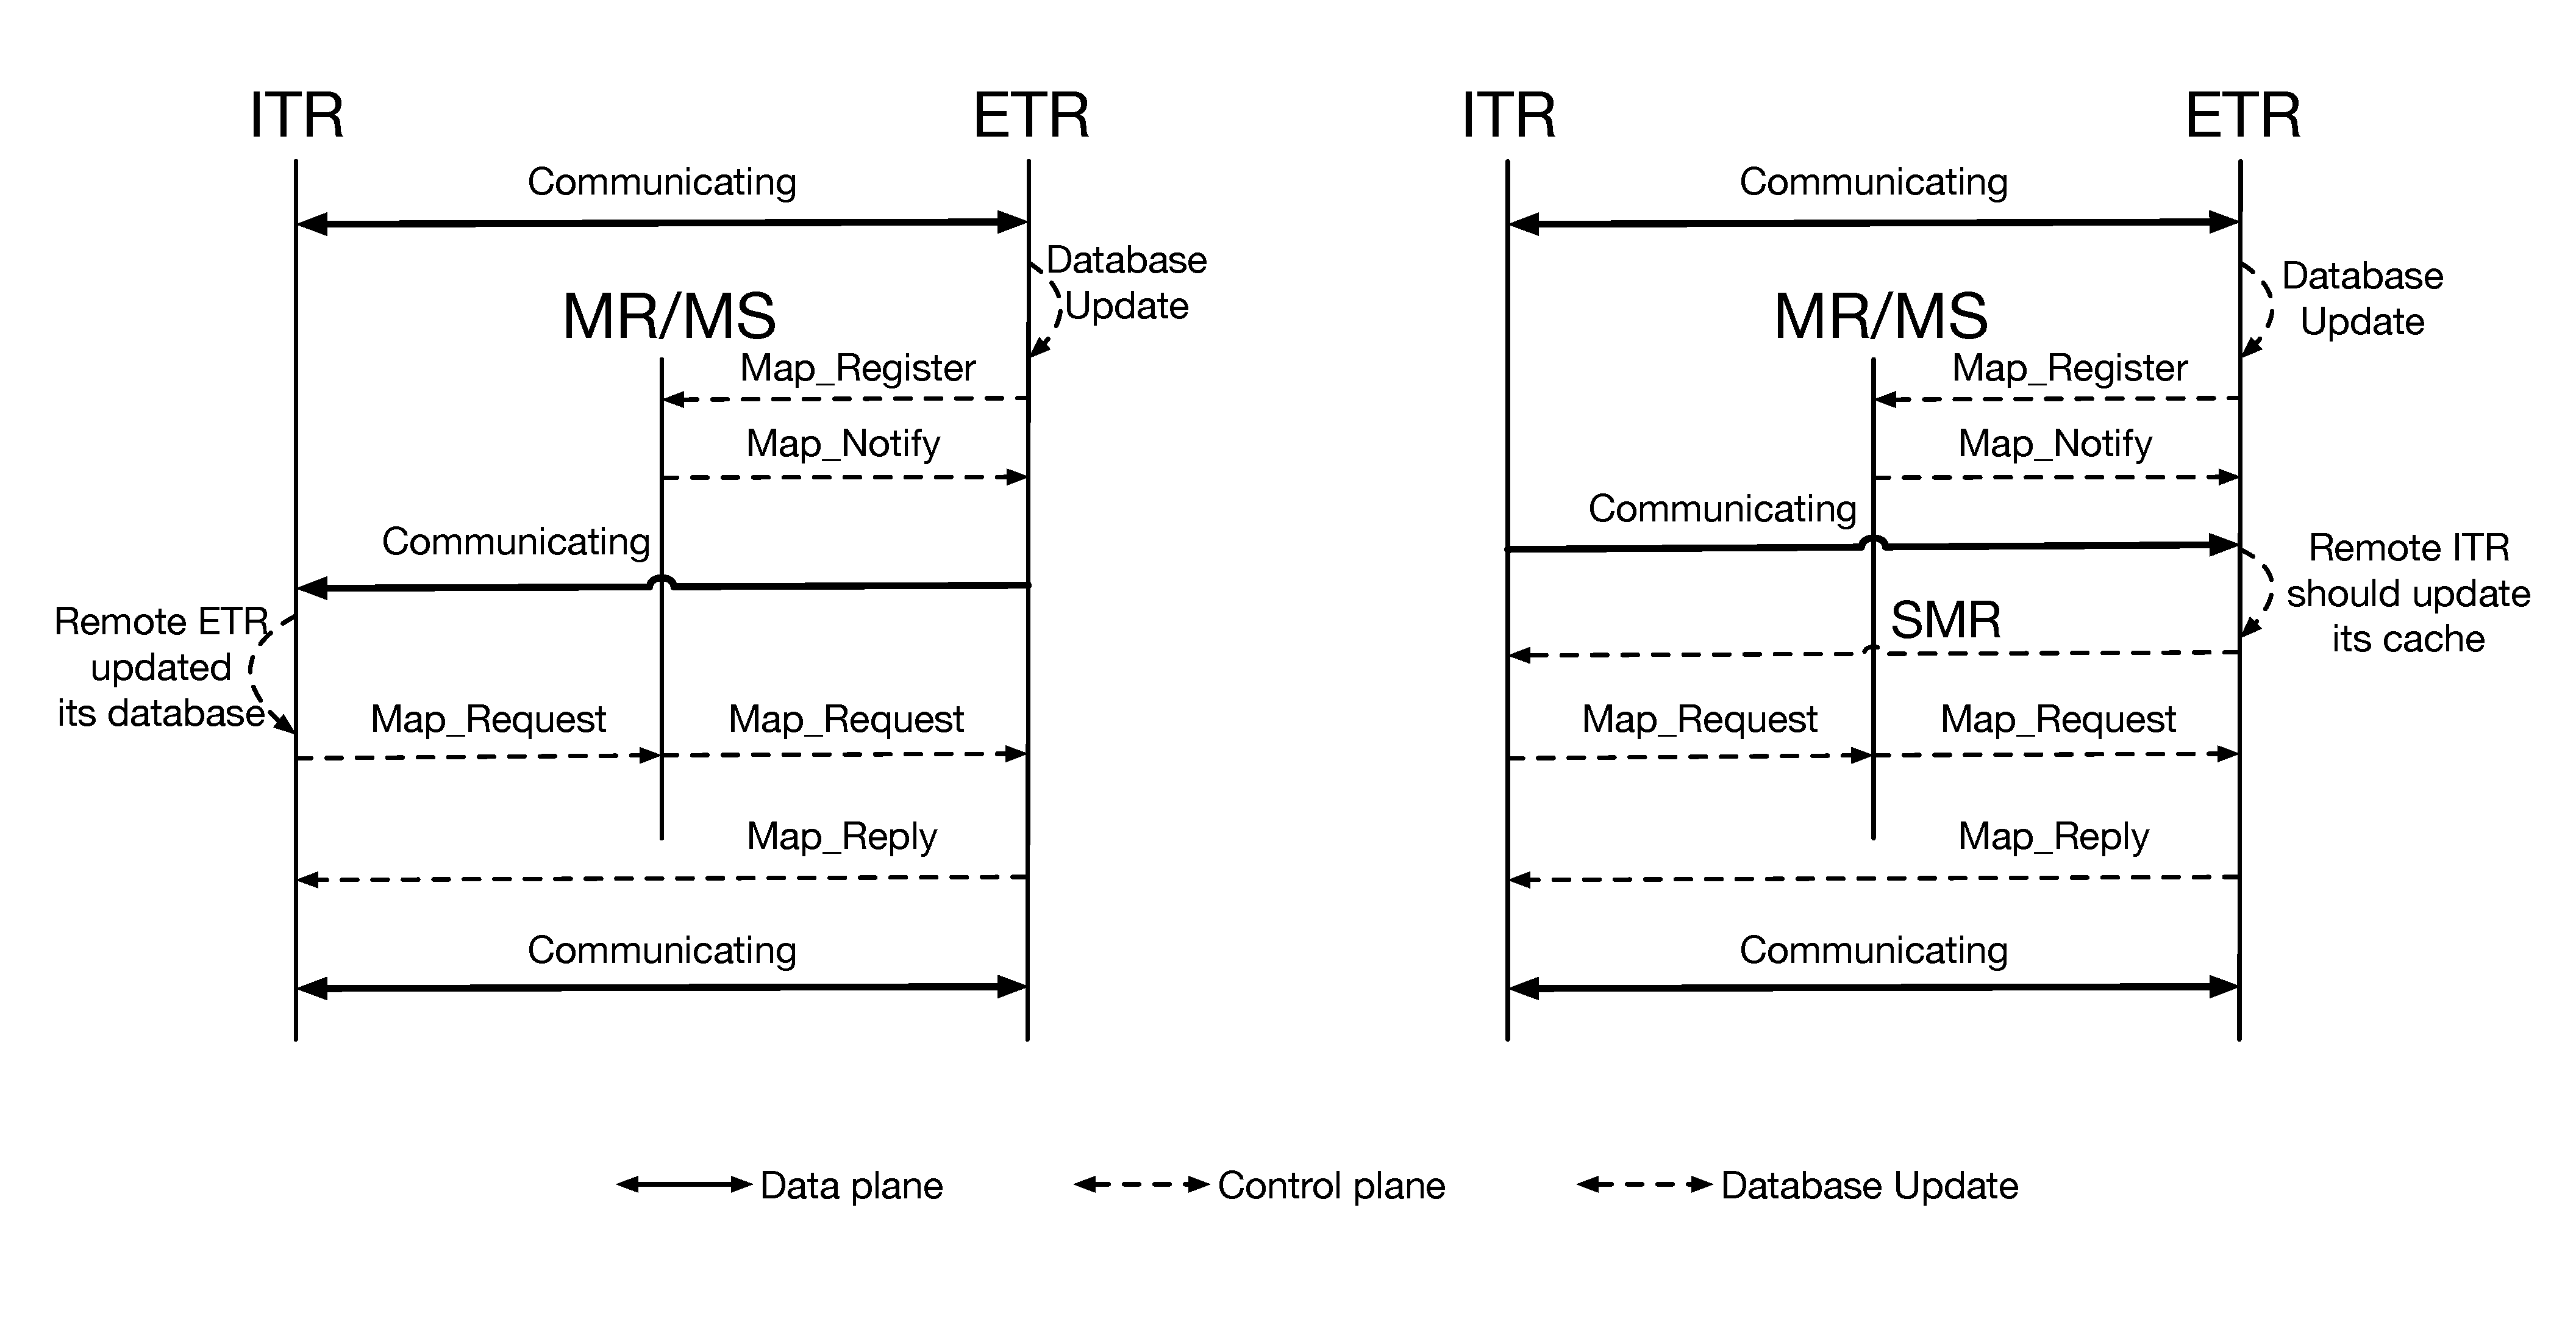
\includegraphics[width=\textwidth]{Pics/Map_versioning_schema.eps}
	\caption{Packet sequence of LISP Map-Versioning mechanism}
	\label{Map_versioning_schema}
\end{figure}
%-< END FIGURE >--------------------------------------------------------------------
Map-Versioning is used to inform through the Data Plane the \acrshort{xtr} that the mappings of a remote site changed and update the mapping information with the help of \acrshort{smr} message. Map-Versioning associates a Map-Version number to each LISP mapping information and transports such a version number in the LISP-specific header~\cite{rfc6834}. When a mapping changes, a new version number, normally incrementally higher than the previous one, is assigned to the updated mapping. When an \acrshort{itr} encapsulates a packet, it selects the version number assigned to the mapping stored in the Database as \emph{source RLOC version number}, and selects the version number assigned to the mapping contained in the Cache as \emph{destination RLOC version number}. When an \acrshort{etr} receives such packets and dencapsulates them, it makes a comparison between the received version number and the local one. If the source map version is higher than the one that \acrshort{etr} stores in its Cache, i.e., the mappings of remote \acrshort{itr} changed, the \acrshort{etr} sends a Map-Request to the MR or directly to the remote \acrshort{itr} to retrieve the latest mapping information (the left figure of Fig.~\ref{Map_versioning_schema}). If the destination map version is lower than the one contained in the Database of \acrshort{etr}, i.e., the local mappings changed but the remote site does not know, then the \acrshort{etr} sends a SMR to the remote \acrshort{itr} to let it update the cached mapping (the right figure of Fig.~\ref{Map_versioning_schema}).


%-< SECTION >--------------------------------------------------------------------
\section{LISP Mobility}
\label{sec:lisp_mobility}
%%-< SUBSUB SECTION >--------------------------------------------------------------------
%\subsection{Mobility at client-side}
%\label{subsubsec:mobility_user}
Nowadays, the explosion of mobile devices that need the massive mobile Internet traffic requires the evolution of mobile network architecture. Keeping the communication during the roaming without any interruption becomes a key point. Thanks to LISP separating the identifier of a host and the locator of the attachment point, the connection between two hosts can be kept alive while roaming. Because the EID, which is used as the inner address, is permanent, whereas only RLOC (used as the outer address) is changed. 

By using LISP mobility, it is possible 
\begin{inparaenum}[1)]
	\item to allow TCP connections to stay alive while roaming;
	\item to provide the shortest bidirectional data paths between a \acrfull{mn} and \acrfull{cn};
	\item to allow \acrshort{mn} to communicate with another \acrshort{mn} when both are roaming;
	\item not require fine-grained routes in the core network, nor the home-agent, foreign agent or other data plane network elements to support mobility;
	\item there is no triangle routing of data packets as is found in Mobile IP~\cite{perkins2002rfc3344};
	\item and there is no IPv6 new extension headers to avoid triangle routing~\cite{johnson2004rfc}.
\end{inparaenum}
\acrfull{lispmn} takes advantage of the LISP infrastructure so to overcome the limits imposed by Mobile IP. % LISP mobility can be applied in 5 scenarios and the 
The implementation of \acrshort{lispmn} is achieved by OOR (Open Overlay Router)~\cite{OOR}, which will be introduced in Sec.~\ref{subsubsec:implementation_oor}.
%\begin{enumerate}[noitemsep,topsep=0pt]
%	\item \acrshort{lispmn} to a \acrfull{lispsn};
%	\item \acrshort{lispmn} to a Non-\acrshort{lispsn};
%	\item \acrshort{lispmn} to another \acrshort{lispmn};
%	\item Non-LISP Site to a \acrshort{lispmn};
%	\item LISP Site to \acrshort{lispmn}.
%\end{enumerate}

LISP can be implemented on both border routers and terminals. % As presented in Sec.~\ref{sec:data_plane}, a router supporting LISP called \acrshort{xtr} and a mobile host supporting LISP called \acrfull{lispmn}, which will be introduced in Sec.~\ref{subsec:lispMN}. 
According to the adoption of LISP and host/router supports LISP, mobility can be divided into 4 categories: LISP-MN in LISP-Site, LISP-MN in non-LISP-Site, MN in LISP-Site, and MN in non-LISP-Site (shown in Tab.~\ref{mobility_catalogs}). However, the case "MN in non-LISP-Site" is the current conventional mobility, which has no relationship with LISP. There are some proposals to solve the seamless mobility issues for the traditional handover, such as Mobile IP (MIP)~\cite{perkins1997mobile}, Mobility Support in IPv6 (MIP6)~\cite{perkins2011mobility}~\cite{minolisecurity}, Multipath TCP (MPTCP)~\cite{ford2013tcp} and so on. Thus, in the following sections, we will present \acrshort{lispmn} first and then only describe how the packets exchange when the handover occurs for the first three cases.

%-< TABLE >-----------------------------------------------------------------
\begin{table}[!tb]
    \centering
    \caption{Catalogs of mobility}
    \label{mobility_catalogs}{
    % \resizebox{0.8\textwidth}{!}{%
        \begin{tabular}{@{}c|c|c@{}}
			\hline\hline
    		Name of catalogs & MN  & Site    	\\  \hline 
    		LISP-MN in LISP-Site & LISP  & LISP    	\\  \hline 
    		LISP-MN in non-LISP-Site & LISP  & non-LISP    	\\  \hline    
    		MN in LISP-Site & non-LISP  & LISP    	\\  \hline    
    		normal mobility & non-LISP  & non-LISP    	\\  \hline \hline                   
    	\end{tabular}
    }
\end{table}
 %-< END TABLE >-----------------------------------------------------------------


%-< SUBSECTION >--------------------------------------------------------------------
\subsection{LISP Mobile Node}
\label{subsec:lispMN}
% \begin{itemize}[noitemsep,topsep=0pt]
%     \item What's LISP-MN.
%     \item How it implements.
%     \item Present an example of packets exchange between LISP-MN and the remote node.
% \end{itemize}
% The forementioned LISP-speaking hosts we discussed are stationary terminals in a LISP-site. 
This section introduces a mobile LISP-speaking node, called \acrfull{lispmn}. It can reside behind both LISP-Site and non-LISP-Site. It is able to change its attachment point during the communication. The \acrshort{lispmn} implements a subset of the standard \acrshort{xtr} functionality~\cite{mn00}. It can send Map-Request to MR to get the mapping information of the remote host.

%-< FIGURE >--------------------------------------------------------------------
\begin{figure}[!t]
	\centering
	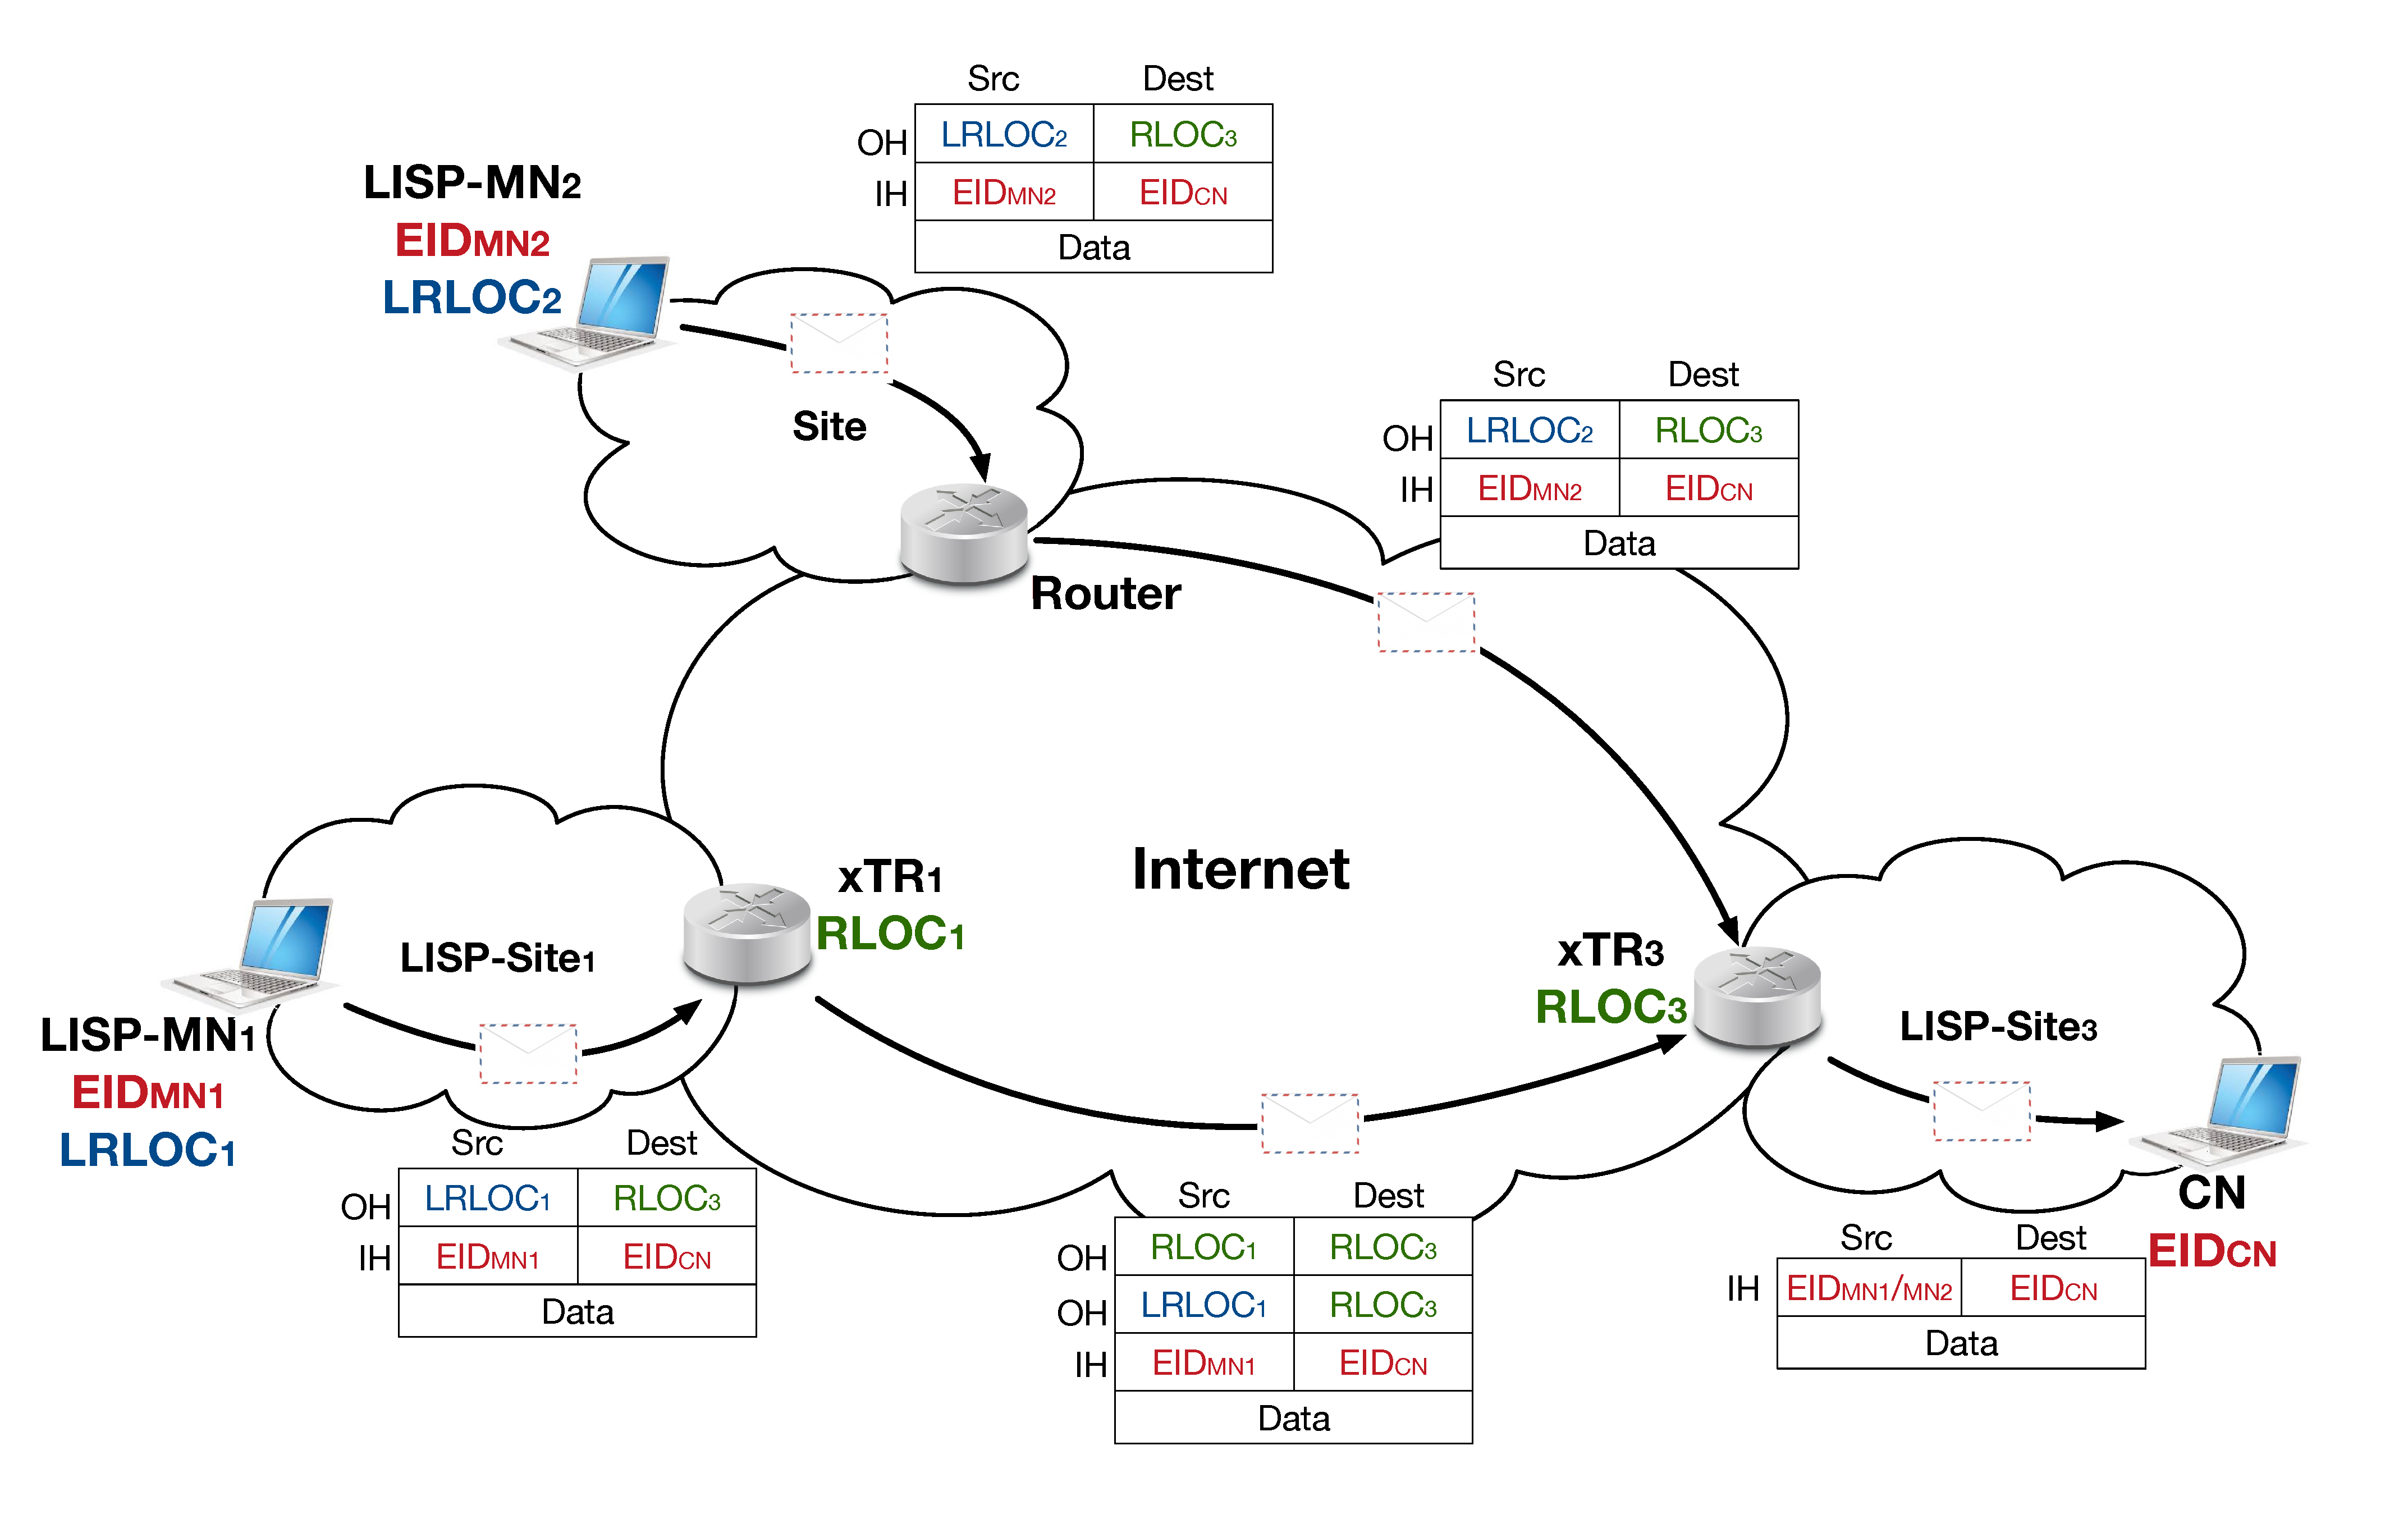
\includegraphics[width=\textwidth]{Pics/LISP-MN_archi.eps}
	\caption{Illustration of LISP-MN in LISP-Site and non-LISP-Site}
	\label{LISP_archi_2encap}
\end{figure}
%-< END FIGURE >--------------------------------------------------------------------
When a LISP-MN resides in a LISP-Site, it is assigned an EID taken from the site's EID-prefix as its RLOC, called \emph{\acrfull{lrloc}}. Thus, LISP-MN stores not only its permanent unique EID but also the \acrshort{lrloc} and registers this mapping information to the \acrshort{ms}. The conventional IP packets produced by the \acrshort{lispmn} are encapsulated by itself using the permanent EID as the inner source address and \acrshort{lrloc} as the outer source address. The encapsulated LISP packets are forwarded to \acrshort{xtr}s and encapsulated again. % by the method of basic LISP encapsulation. % The procedure of packets being encapsulated two times are called \emph{LISP double encapsulation}.

When a LISP-MN resides in a non-LISP-Site, it is assigned an IP address taken from the site's prefix as its \emph{\acrshort{lrloc}}. LISP-MN also need to store both its permanent unique EID and the \acrshort{lrloc} and register this mapping information to the \acrshort{ms}. The conventional IP packets produced by the \acrshort{lispmn} are encapsulated by itself using the permanent EID as the inner source address and \acrshort{lrloc} as the outer source address. The encapsulated LISP packets are forwarded to the border router and natively forwarded to the Internet core. 

The packet flow sequence of \acrshort{lispmn} in LISP-Site and non-LISP-Site are shown in Fig.~\ref{LISP_archi_2encap}. Two \acrshort{lispmn}s, i.e., $\text{LISP-MN}_1$ and $\text{LISP-MN}_2$ send the packets to a remote \acrfull{cn} . The only difference is that $\text{LISP-MN}_1$ resides in a LISP-Site, while $\text{LISP-MN}_2$ resides in a non-LISP-Site. The $\text{LISP-MN}_1$ produces the traditional IP packets with $EID_{MN1}$ as source address and $EID_{CN}$ as destination address. Then it encapsulates by adding $LRLOC_1$ as outer source address and $RLOC_3$ as outer destination address by itself after querying the mapping information. The LISP packets with one time encapsulation are forwarded to $xTR_1$. The latter gets the mapping information from \acrshort{mr} and encapsulates once again the packets by adding the $RLOC_1$ as the outer source address and $RLOC_3$ as the outer destination address, then sends the double LISP encapsulated packets on core Internet. The $xTR_3$ needs to dencapsulate the packets twice after receiving and verifying the packets, and finally sends to $CN$.

The situation for $\text{LISP-MN}_2$ is simpler. It also produces the traditional IP packets and encapsulates the packets by itself, then sends to its border router. The $Router$ does nothing related to LISP but only forwards the already LISP-encapsulated packets to the Internet core. Thus, the packets are encapsulated only once, whose inner source and destination address is respectively $EID_{MN2}$ and $EID_{CN}$, outer source and destination address is respectively $LRLOC_2$ and $RLOC_3$.


%-< SUBSECTION >--------------------------------------------------------------------
\subsection{MN mobility in LISP-Site}
\label{subsec:MN_LS}
When the \acrshort{mn} is normal host without any LISP function, while the border router supports LISP, i.e., \acrshort{xtr}, the packets are exchanged with the remote $CN$ as the basic communication between two LISP-Sites introduced in Sec.~\ref{sec:communication_2_lisp}. The \acrshort{eid} of \acrshort{mn} is distributed from the EID-prefix of the LISP-Site, if \acrshort{mn} moves to a new LISP-Site but keeps the original \acrshort{eid}, it can not exchange the packets with its new \acrshort{xtr}, since its \acrshort{eid} does not belong to the EID-prefix of the new LISP-Site. Thus, in this case, the mobility of \acrshort{mn} can only conduct within a subnet instead of roaming through different domains.


%-< SUBSECTION >--------------------------------------------------------------------
\subsection{LISP-MN mobility in LISP-Site}
\label{subsec:lispMN_LS}

%-< FIGURE >--------------------------------------------------------------------
\begin{figure}[!t]
	\centering
	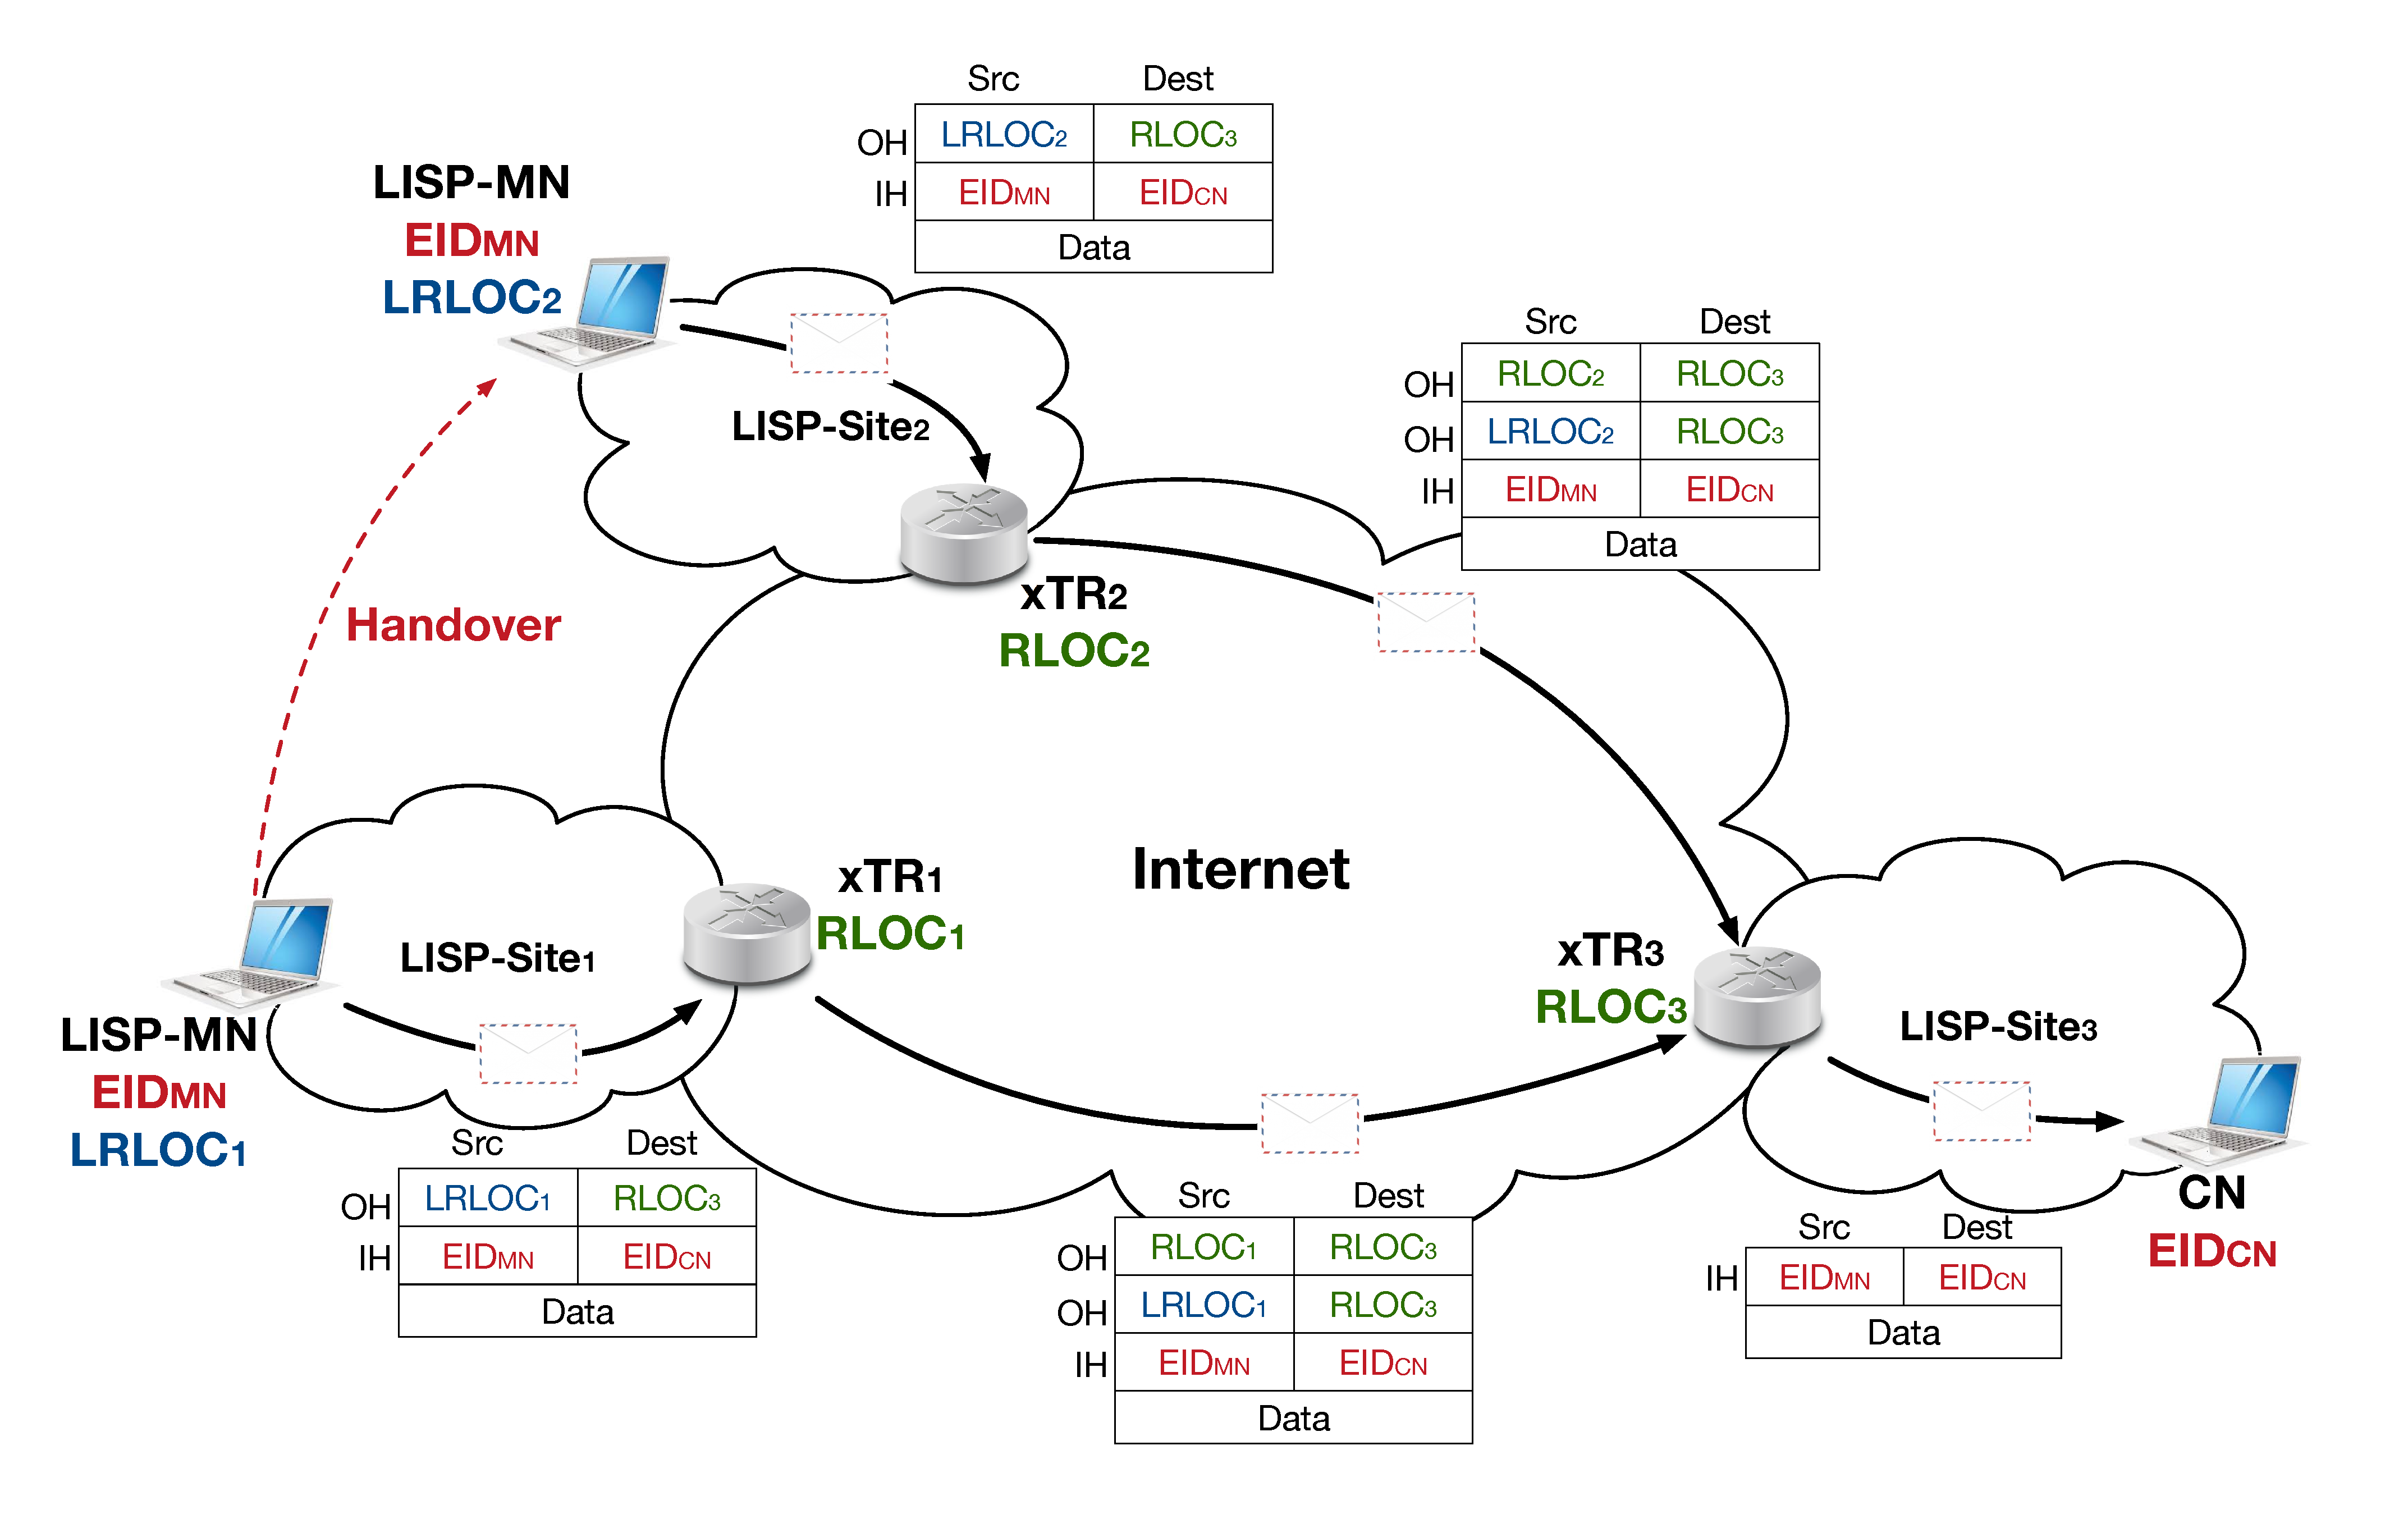
\includegraphics[width=\textwidth]{Pics/LISP-MN_in_LISP-Site.eps}
	\caption{Packet flow of mobility when LISP-MN in LISP-Site}
	\label{LISP-MN_in_LISP-Site}
\end{figure}
%-< END FIGURE >--------------------------------------------------------------------

This section describes how a \acrshort{lispmn} moves from one LISP-Site to another and the packet flow is shown in Fig.~\ref{LISP-MN_in_LISP-Site}. At first, packets exchanged between $\text{LISP-MN}$ residing in $\text{LISP-Site}_1$ and $CN$ are double encapsulated LISP packets as mentioned in Sec.~\ref{subsec:lispMN}. After conducting the handover, $\text{LISP-MN}$ still uses its permanent $EID_{MN}$. However, since it changes the attachment point, $xTR_2$ distributes a new EID from its EID-prefix to it, and it uses this as its new \acrshort{lrloc}, labeled $LRLOC_2$ in the figure. The $\text{LISP-MN}$ should register itself with the new mapping information to the \acrshort{mds} and ask $CN$ to update its LISP-Cache by \acrshort{smr} or Map-Versioning (introduced in Sec.~\ref{sec:updateMechanisms}). When receiving the packets from $\text{LISP-MN}$, the $xTR_2$ conducts the second encapsulation and sends the packets to $xTR_3$. The benefit of such mobility is that the $\text{LISP-MN}$ can roam through the different subnets without interrupting the communication with the remote $CN$, because $\text{LISP-MN}$ never changes its EID. However, to conduct double registration may lead to higher delay of handover.

%-< SUBSECTION >--------------------------------------------------------------------
\subsection{LISP-MN mobility in non-LISP-Site}
\label{subsec:lispMN_NLS}

%-< FIGURE >--------------------------------------------------------------------
\begin{figure}[!t]
	\centering
	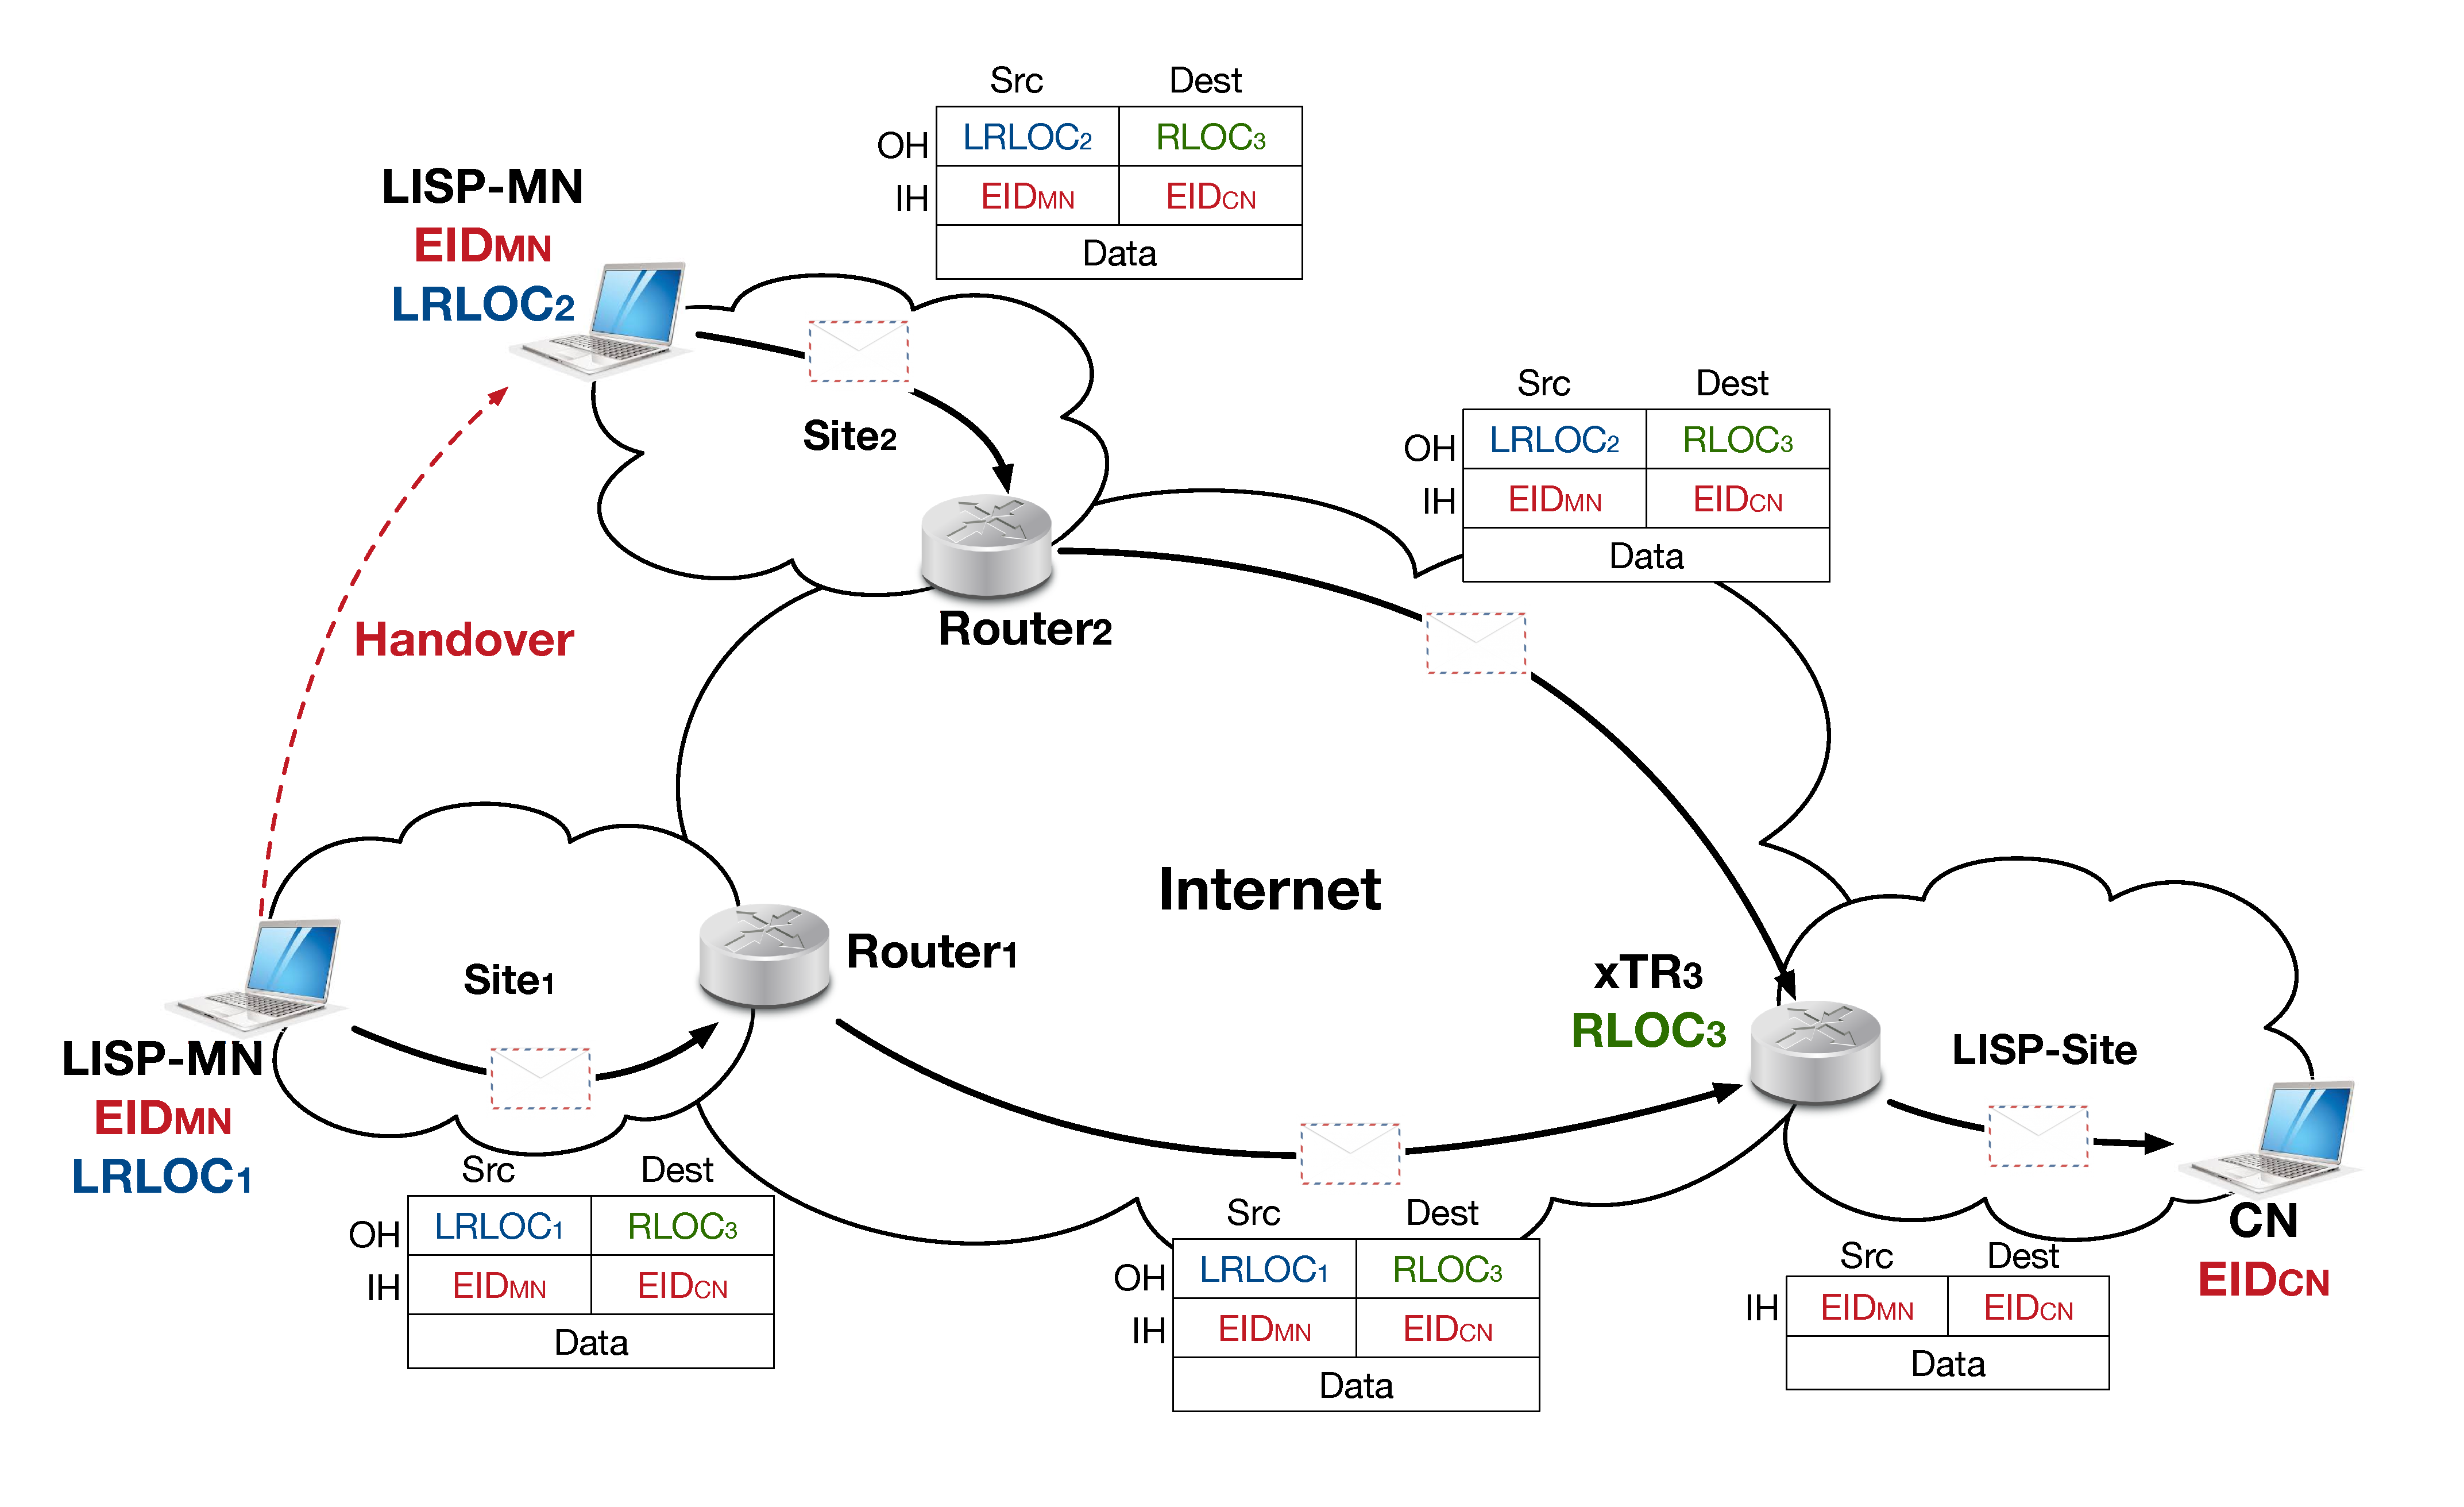
\includegraphics[width=\textwidth]{Pics/LISP-MN_in_non-LISP-Site.eps}
	\caption{Packet flow of mobility when LISP-MN in non-LISP-Site}
	\label{LISP-MN_in_non-LISP-Site}
\end{figure}
%-< END FIGURE >--------------------------------------------------------------------
The Fig.~\ref{LISP-MN_in_non-LISP-Site} illustrates the packet flow of the $\text{LISP-MN}$ roaming between two non-LISP-Sites. The $Site_1$ distributes an IP address from its prefix to $\text{LISP-MN}$, and the later uses this as its \acrshort{lrloc}, labeled as $LRLOC_1$ in the figure. The $\text{LISP-MN}$ encapsulates the packets by itself and sends to $Router_1$. $Router_1$ just natively forwards the packets to $xTR_3$. When $\text{LISP-MN}$ moves to another site labeled $Site_2$, it receives an IP address from a different prefix and uses it as the new \acrshort{lrloc}. It registers itself to the \acrshort{mds} with the $EID_{MN}\text{-to-}LRLOC_2$, and informs the remote $CN$ to update the mapping information by sending \acrshort{smr} or using Map-Versioning. In this scenario, $\text{LISP-MN}$ can also permit to roam through the different subnets, but it can also reduce the high latency of double registration during the handover. 


 %-< SUBSECTION >--------------------------------------------------------------------
 \subsection{LISP-MN mobility between LISP-Site \&  non-LISP-Site}
 \label{subsec:MN_NLS}

%-< SUB SECTION >--------------------------------------------------------------------
\section{LISP alternative use-cases}
\label{subsec:studies_usecase}
% State LISP use-cases
%     \begin{itemize}[noitemsep,topsep=0pt]
%         \item Traffic Engineering~\cite{rfc7834}
%         \item Transmission Between IPv4 and IPv6~\cite{rfc7834}
%         \item Mobility at User-side \yue{Cisco: Locator ID Separation Protocol (LISP) VM Mobility Solution, Support for Network-based User Mobility with LISP}
%         \item Mobility in Data Center \yue{Patrick's thesis + Cisco solution}
%         \item LISP SDN~\cite{barkai2017lisp}~\cite{han2016design}
%     \end{itemize}
Even though LISP is proposed to solve the Internet scalability issues, it also provides the advantages to the other uses, such as: traffic engineering, transition between IPv4 and IPv6, device's mobility at client-side, virtual machine's mobility in data center, LISP SDN, and so on~\cite{rfc7834}. 

%-< SUBSUB SECTION >--------------------------------------------------------------------
\subsection{LISP traffic engineering}
\label{subsubsec:te}
For every mapping information, an EID-prefix associates to a list of RLOC tuples $<$RLOC, Priority, Weight$>$, where each RLOC is annotated with a priority and a weight. In the case of multiple RLOCs existing, the ITR selects the one with the highest priority and sends all the LISP encapsulated packet to this RLOC. If several RLOCs all have the highest priority, the traffic is balanced proportionally according to their weight among such RLOCs so to route to multiple ETRs. Traffic engineering in LISP thus helps the mapping owner decide the primary and backup path for its incoming packets, and also allows it to control the traffic load among its links. For example, the received Map-Reply shows that an EID-prefix is associated to $<$RLOC\_1, 10, 50$>$, $<$RLOC\_2, 10, 20$>$, $<$RLOC\_3, 10, 20$>$, $<$RLOC\_4, 10, 10$>$, then the RLOC\_1 gets 50\% of the traffic, RLOC\_2 and RLOC\_3 are respectively assigned to 20\% of the traffic, and the last 10\% of the traffic are balanced by RLOC\_4.  % An example of the use of such a feature is described by Saucez et al. [SDIB08], which shows how to use LISP to direct different types of traffic on different links having different capacity.

Traffic engineering in LISP can achieve one step further than nowadays BPG. Since every Map-Request contains the source EID of the packet, for which causes the ITR mapping miss and triggers the Map-Request. It is possible that a mapping owner (ETR) gives the different Map-Replies according to the sender of Map-Requests. Thus, the traffic engineering policy may be different to different ITRs although they query the same ETR for the same EID-prefix. This functionality is not available today with BGP, because a domain cannot control exactly the incoming routes from the other domains if they are not direct neighbor.


%-< SUBSUB SECTION >--------------------------------------------------------------------
\subsection{LISP transition between IPv4 and IPv6}
\label{subsubsec:transmission}
The LISP encapsulation mechanism is designed to support any combination of address families for locators and identifiers, such as: IPv4, IPv6, MAC address, or some other arbitrary elements. It is then possible to bind IPv6 EIDs with IPv4 RLOCs and vice versa. This allows transporting IPv6 packets over an IPv4 network (or IPv4 packets over an IPv6 network) by deploying the xTRs at the border of heterogeneous networks, making LISP a valuable mechanism to ease the transition to IPv6.
%-< FIGURE >--------------------------------------------------------------------
\begin{figure}[!t]
	\centering
	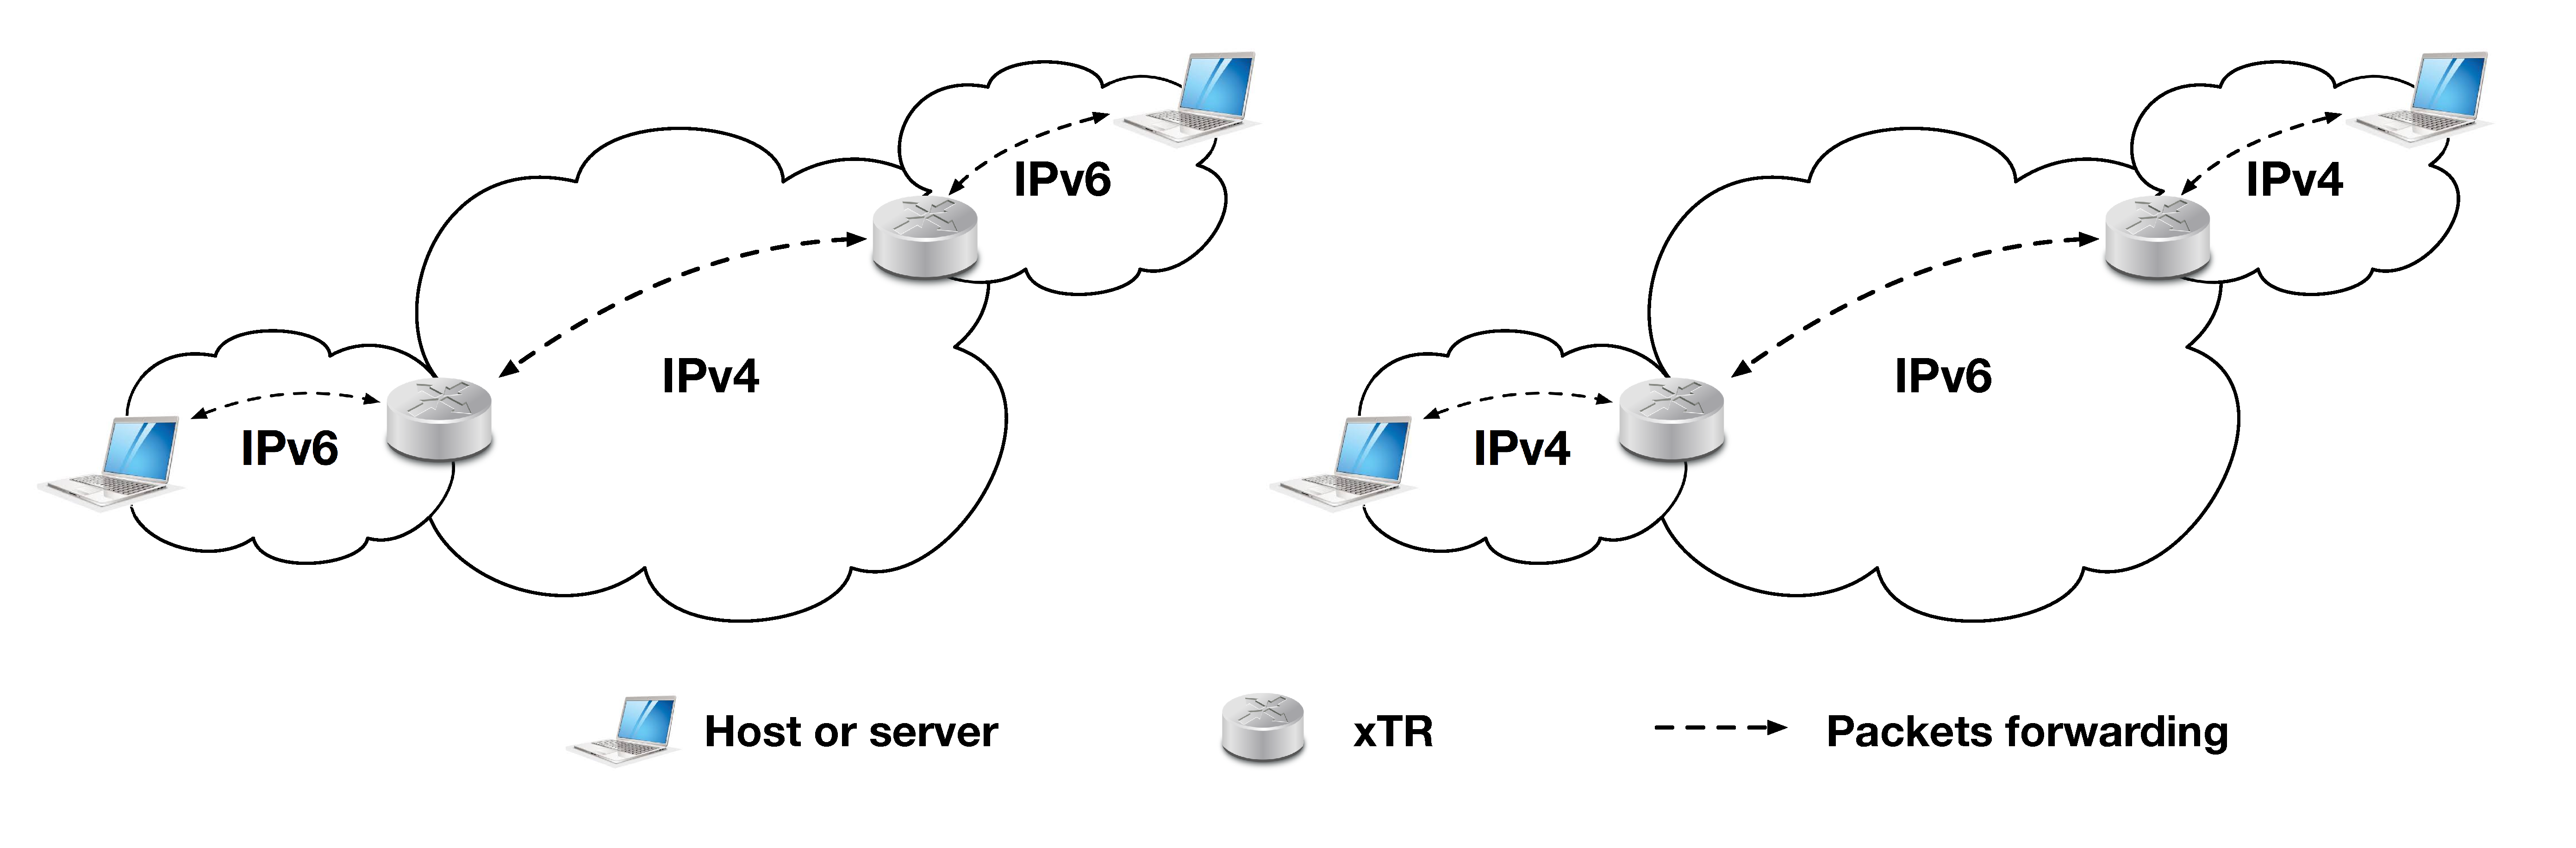
\includegraphics[width=\textwidth]{Pics/transmission_ipv4_ipv6.eps}
	\caption{Illustration of LISP transmission between IPv4 and IPv6}
	\label{transmission_ipv4_ipv6}
\end{figure}
%-< END FIGURE >--------------------------------------------------------------------

Examples are as shown in Fig.~\ref{transmission_ipv4_ipv6}, where IPv6 islands are connected via IPv4 infrastructure (on the left) and IPv4 islands are connected through IPv6 infrastructure (on the right). As LISP provides mechanisms for encapsulating IPv6 host packets using IPv4 RLOCs on the xTRs, LISP can then provide IPv6 communication between hosts/servers even though the intermediate network only supports IPv4. Similarly, xTR can encapsulate the IPv4 packets by adding the IPv6 RLOCs to achieve the IPv4 access through the IPv6 infrastructure. In addition, when the LISP infrastructure includes PxTRs, it can provide both IPv4 and IPv6 connectivity to non-LISP IPv4/IPv6 sites (legacy Internet). In summary, it can function in any of four following ways:
\begin{itemize}[noitemsep,topsep=0pt]
	\item IPv4-to-IPv4 over IPv4
	\item IPv4-to-IPv4 over IPv6
	\item IPv6-to-IPv6 over IPv4
	\item IPv6-to-IPv6 over IPv6
\end{itemize}
However, LISP does not translate between the IPv4 and IPv6 EIDs.



%%-< SUBSUB SECTION >--------------------------------------------------------------------
%\subsection{Mobility in Data Center}
%\label{subsubsec:mobility_DC}
%As the server virtualization and high availability across geographically dispersed data centers are more and more common, similar to the realization of LISP mobility at client-side, the migration of \acrfull{vm} within a data center or from a data center to another without dropping the running connections also becomes a potential use case of LISP. Two mechanisms at the state of the art can perform this operation. One is the aforementioned host-based LISP implementation called OOR, another method to handle \acrshort{vm} mobility via LISP is actually implemented in some Cisco products, only partially documented in~\cite{ciscovmmobility}. % The later one will be presented here.
%
%% The proposal of Cisco is based on the decoupling of Identifier from the topology so to ensure the changing of attachment point does not affect the EID. In the LISP VM-Mobility solution, only border routers of data center are embedded LISP, whereas VM is not, unlike \acrshort{lispmn}. When a VM moves to another subnet (i.e., it is paused, copied to another location, and then resumed), the VM restarts the DHCP procedure in order to obtain an suitable IP address for the new network. It does not continue to send traffic using the old IP, since it realizes that its attachment point has changed. As soon as the new xTR receives the DHCP, it realizes a VM moving from another subnet to its (i.e., it is paused, copied to another location, and then resumed) by detecting that the source IP of the traffic is not part of its EID-prefix (but it’s an allowed EID). The movement of VM is thus dynamically detected by xTR (the new LISP-VM router). After the new LISP-VM router detecting the newly moved-in VM, the new xTR needs to register the /32 for the VM's EID using its RLOC(s), and update the \acrshort{ms} by sending the Map-Register. Then, the MS replies 2 Map-Notifies: one is the acknowledge of Map-Register to the new xTR (the one who sent the Map-Register); the other one is to inform the previous xTR (which RLOCs were previously mapped to the VM's EID) to remove the mapping information for the leaving VM. Then, the previous xTR notifies the departure of VM by sending SMRs to every CN, which was communicating with the moved VM before. By updating the RLOC-to-EID mappings, traffic is redirected to the new locations without causing any churn in the underlying routing. As the VM is not aware of the move during the whole roaming, the LISP VM-Mobility solution is network-based mobility.


%-< SUBSUB SECTION >--------------------------------------------------------------------
\subsection{LISP SDN}
\label{subsubsec:sdn}
As described before, LISP is inherently decoupling Control Plane from Data Plane. LISP moves all control functions onto Mapping System, while keeps data functions at the xTR level.%\yue{Personally, I'm not agreed with this statement. Your writing makes me feel that xTR only supports data plane function. Actually it also support control plane functions...}
The feature of LISP corresponds to the characteristic of \acrfull{sdn}, which also decouples Network Control Plane from Data Plane, increases flexibility and development speed of features and functionalists. Thus, this decoupling entitles network operators to build a \acrfull{sdn} on top of LISP~\cite{rodriguez2014software}.

%-< FIGURE >--------------------------------------------------------------------
\begin{figure}[!t]
	\centering
	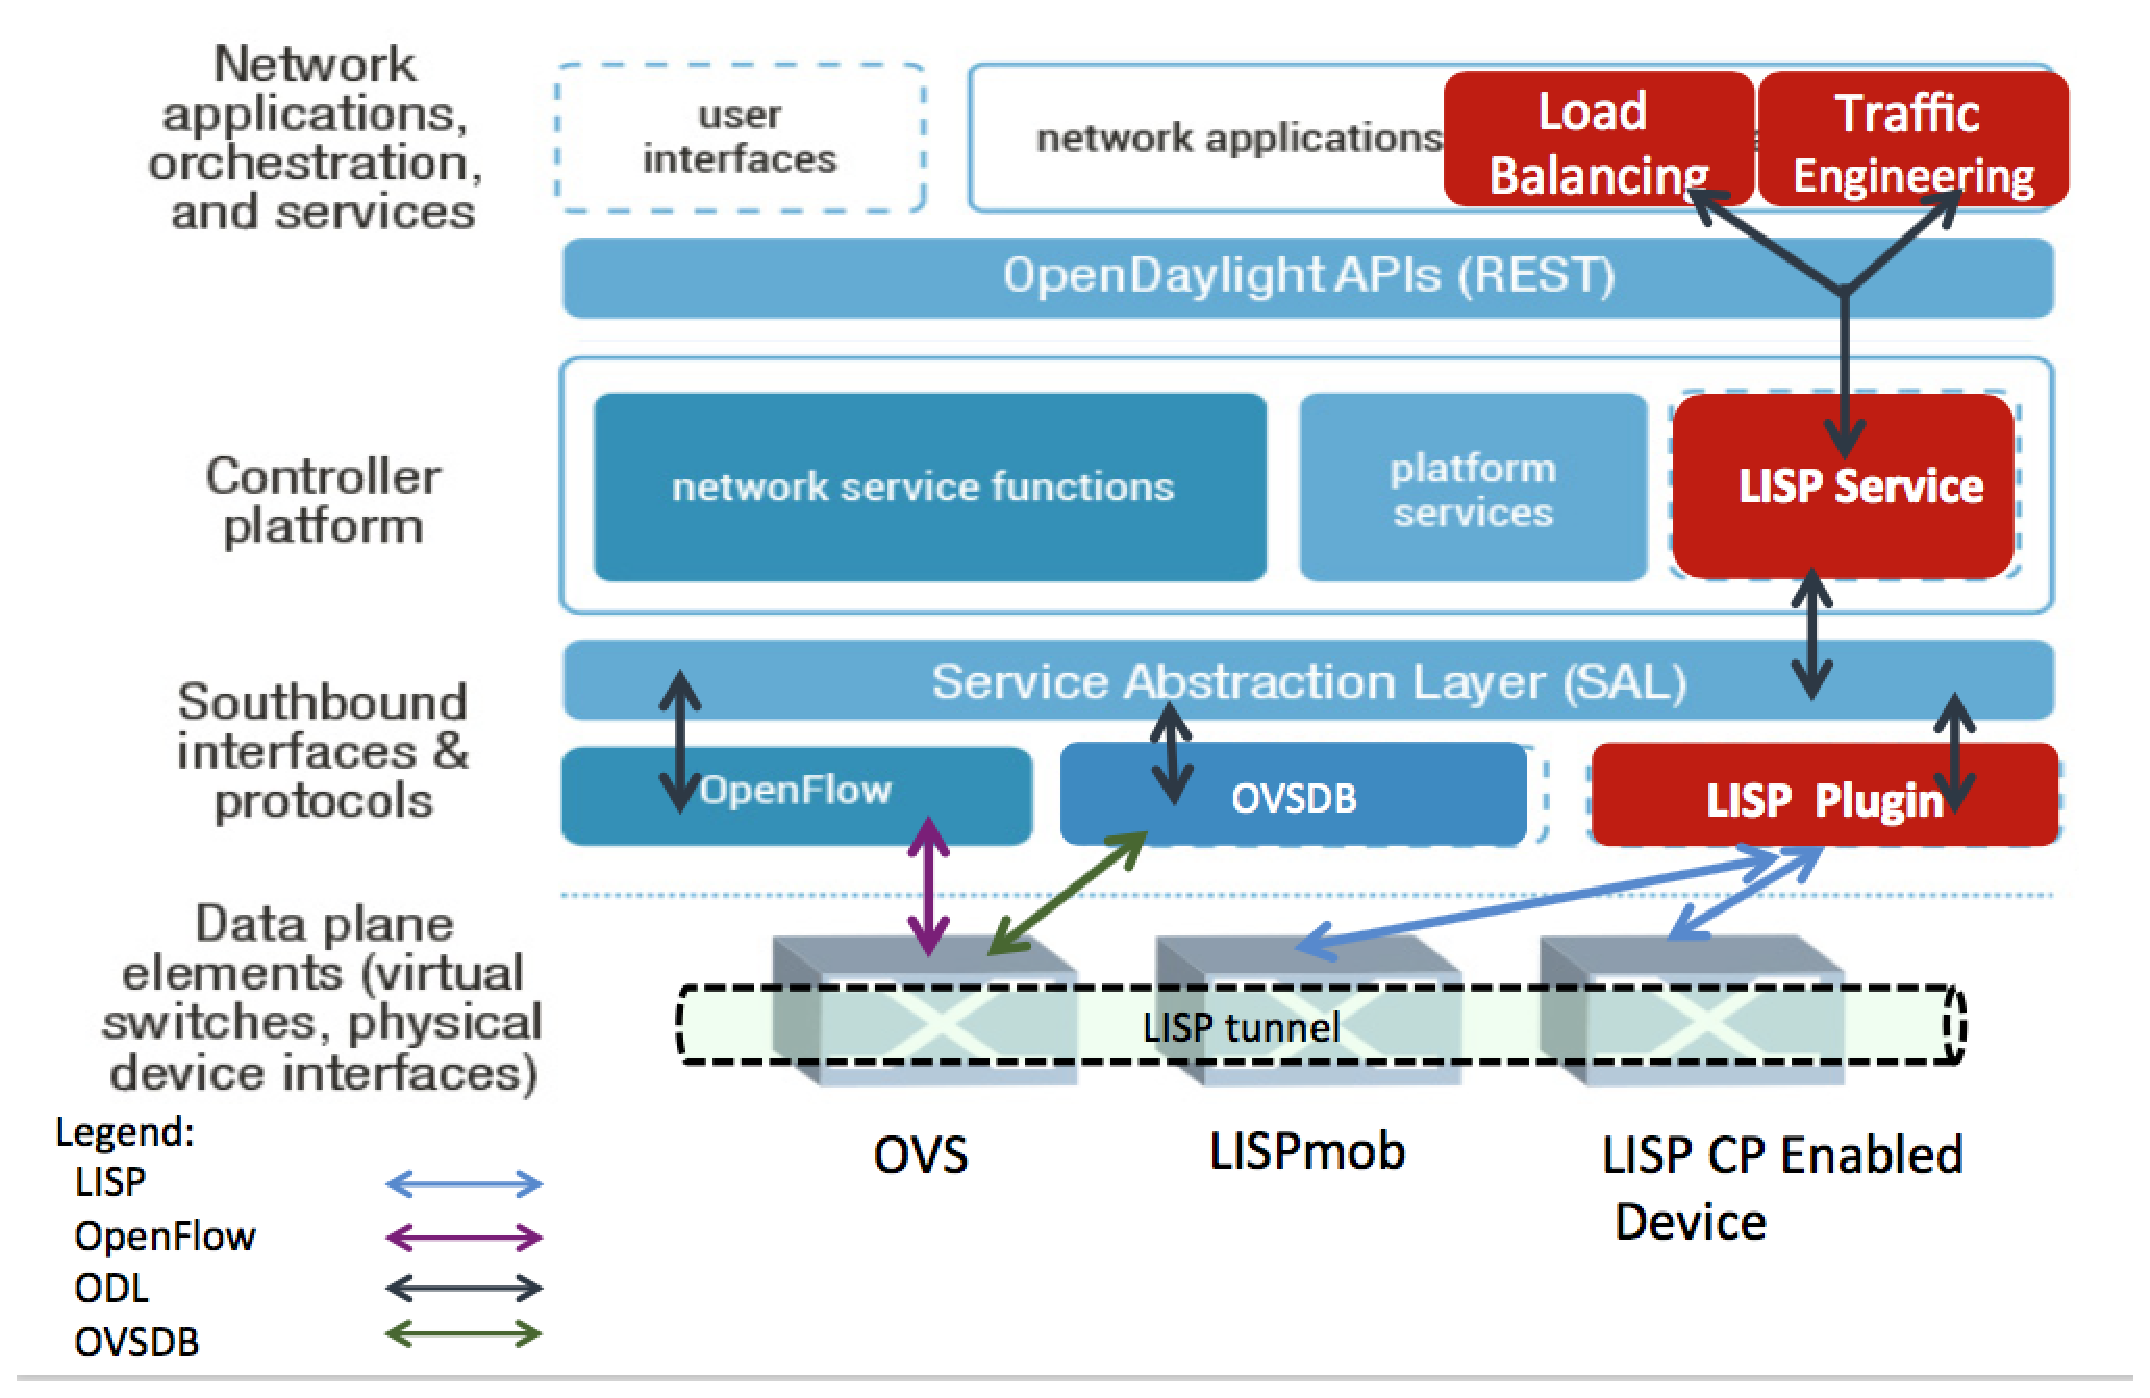
\includegraphics[width=\textwidth]{Pics/LISP_in_OpenDaylight.eps}
	\caption{LISP in OpenDaylight (source:~\cite{LISP_ODLSummit_2014})}
	\label{LISP_in_OpenDaylight}
\end{figure}
%-< END FIGURE >--------------------------------------------------------------------
The OpenDaylight Project~\cite{OpenDaylight} is a collaborative open source project hosted by The Linux Foundation to promote \acrfull{sdn} and \acrfull{nfv}. It implements the LISP Control Plane functions as shown in Fig~\ref{LISP_in_OpenDaylight}. The data plane elements consist of virtual switches and physical device interfaces, at the aim of constructing the LISP tunnel to transfer the packets. The LISP Plugin is the Southbound interface, which is used to look up LISP policies from LISP Service by sending Map-Request and receiving Map-Reply, and create the LISP tunnel over LISP overlay across the different kinds of data plane devices. The LISP Service is actually implemented as LISP Mapping System to store the various user-defined policies. The only difference is that in OpenDaylight, it is the \acrshort{ms} itself that replies to the Map-Requests, instead of forwarding them to any xTR. It is like every mapping has the "proxy Map-Reply" flag (P-bit) set to response on behalf of xTRs. The OpenDaylight APIs (REST) are used to set the policies, such as: the policies for Load Balancing and Traffic Engineering, obtained from the north bound into LISP Service. The policies are defined as the network applications or services by the users.

Network functions such as subscriber-management, content-optimization, security and quality of service, are typically delivered using proprietary hardware appliances embedded into the network~\cite{barkai2017lisp}. But the next generation network functions are being implemented as pure software instances running on standard servers. They are unbundled virtualized components of capacity and functionality. LISP-SDN based flow-mapping, dynamically assembles these components to whole solutions by steering the proper traffic in the right sequence to the correct virtual function instance.
 % Background
%*******************************************************************************
%****************************** Second Chapter *********************************
%*******************************************************************************

\chapter{Related Work}
\label{cha:related_work}

% **************************** Define Graphics Path **************************
\ifpdf
    \graphicspath{{Chapter3/Pics/Raster/}{Chapter3/Pics/PDF/}{Chapter3/}}
\else
    \graphicspath{{Chapter3/Pics/Vector/}{Chapter3/}}
\fi
This chapter first presents the current LISP status, including: two available LISP platforms, the only LISP monitor, two LISP manual management tools, and some private and some open-source implementations. It also introduces the latest research achievements, from the LISP network evolution, the LISP mapping system assessment, the evaluation of interworking between LISP-site and legacy Internet, to the analysis of LISP mobility. Besides presenting the existing works, we also find some limitations in each aspect. Thus, we point out the shortcomings in the LISP monitor and implementations, as well as in the various aspects of LISP performance evaluation. We tackled most of these issues and present them in this dissertation. % The work that we conducted to complete LISP studies are presented in the following chapters, i.e., from Chapter.~\ref{cha:mds_evaluation} to Chapter.~\ref{cha:ns-3}. 
Further, we list some other LISP challenges and issues at the end of this chapter. Although these fields are not considered in this dissertation, they are also important to help researchers improve LISP technology.


%-< SECTION >--------------------------------------------------------------------
\section{LISP platforms}
\label{sec:platform}
This dissertation is focusing on the evaluation of LISP performance in the real environment, thus the large scale experiments on existing platforms are of paramount importance. As such, we introduce first two existing LISP platforms: LISP Beta Network and LISP-Lab platform, before discussing the current research results.

%-< SUB SECTION >--------------------------------------------------------------------
\subsection{LISP Beta Network}
\label{subsec:platform_beta}
% \begin{itemize}[noitemsep,topsep=0pt]
%     \item First global LISP testbed.
%     \item Initiated by Cisco.
%     \item Introduce all its components: how many MR/MS, PxTR, etc.
% \end{itemize}

The first global LISP testbed called LISP Beta Network~\cite{lispbeta}~\cite{coras2014performance}, has been deployed since 2008. Started as the only LISP testbed, the LISP Beta network had a steady growth and achieved world-wide experimental deployment~\cite{lispCCR} with the purpose to gain real-life experience on LISP. Initiated by Cisco, the members of the LISP Beta Network are not only major companies and operators, but also academics, research laboratories, and startups offering LISP related services. Participants of this network are located in 34 different countries, with the highest concentration in Europe and North America.

%-< FIGURE >--------------------------------------------------------------------
\begin{figure}[!t]
	\centering
	\includegraphics[width=\textwidth]{Pics/LISP_Beta_Network_Topology.eps}
	\caption{International LISP Beta Network High Level Topology – October 2017~\cite{lispbetaarchi}}
	\label{LISP_Beta_Network_Topology}
\end{figure}
%-< END FIGURE >--------------------------------------------------------------------
The LISP Beta Network is composed of the mapping system, LISP routers (i.e., xTRs), mobile nodes, Re-encapsulating Tunnel Routers (RTR~\cite{ermagan2016nat}) and Proxy Tunnel Routers (PxTR~\cite{rfc6832}). On March \nth{14} 2012, the mapping system used by the LISP Beta Network has switched from LISP+ALT~\cite{rfc6836} to the more flexible LISP-DDT~\cite{lispDDT}. Changing the  mapping system has considerably reduced the configuration and maintenance burden, while a slight performance degradation has been observed~\cite{lispCCR}. According to the latest architecture (October 2017)~\cite{lispbetaarchi} shown in Fig.~\ref{LISP_Beta_Network_Topology}, LISP Beta Network has 3 DDT Root, 2 DDT TLD, 7 available MR/MSes and 6 PxTRs. More precisely: 2 MR/MSes and 2 PxTRs are in US, 3 MR/MSes and 3 PxTRs are in Europe, 2 MR/MSes and 1 PxTR are in Asia. It mainly uses two EID addressing spaces, which belongs to Cisco: 153.16.0.0/16 for IPv4 and 2610:00D0::/32 for IPv6~\cite{lispCCR}, but there are also some other EIDs. % LISP Beta Network consists of 518 LISP sites\yue{Need to verify if still 518 now}. Although the deployment scope is still limited compared to the Internet, its size is sufficient to conduct reasonable measurement campaigns to understand LISP behavior and performance. 


%-< SUB SECTION >--------------------------------------------------------------------
\subsection{LISP-Lab platform}
\label{subsec:platform_lab}
% \begin{itemize}[noitemsep,topsep=0pt]
%     \item LISP-Lab is an open platform LISP testbed project.
%     \item Opened from 2015.
%     \item Already been interconnected to the LISP Beta Network with an Open-LISP DDT root~\cite{fuller2012lisp}.
% \end{itemize}
Due to a monolithic control by one single commercial actor, however, LISP Beta network has limitations to explore the innovative services. Thus, some other projects, such as ANR LISP-Lab project~\cite{lisplab}, focus on developing new enhanced features.

LISP-Lab project aimed at building an open platform, based on the LISP architecture, providing the environment to perform high quality research and support the design, development, and thorough assessment of new services and use-cases. The range of technical tasks planned in the LISP-Lab project, from cloud networking, to access technology, through inter-domain connectivity, traffic engineering, and mapping management, boosting innovation beyond the LISP technology itself. LISP-Lab platform was solely deployed by using open source LISP implementation, OpenLISP~\cite{OpenLISP}, since 2015. % opened to the external users from 2015. 
It was coordinated by a French consortium: two academic institutions (UPMC, TPT), two Cloud Networking SME (Alphalink, NSS), two network operators (Renater, Orange), two SMEs on Access/Edge Networking (Border 6, Ucopia) and one Internet eXchange Point (Rezopole). Ten international external partners also joined the platform. At the moment of writing, LISP-Lab consists of 3 \acrshort{mr}s/\acrshort{ms}es and 2 PxTRs located in France, as well as 13 worldwide xTRs, and has already been interconnected to the LISP Beta Network with an Open LISP DDT root~\cite{fuller2012lisp}.


%-< SECTION >--------------------------------------------------------------------
\section{LISP monitoring tools}
\label{sec:monitor}
As the researchers need to leverage on LISP tools to conduct the experiments on the aforementioned LISP platforms, this section introduces the currently existing tools to supervise LISP status or troubleshooting it for some specific purposes. % We will explain their working mechanisms and figure out their shortcomings. Also, we will state the necessity and urgency to propose a new comprehensive one.

%-< SUB SECTION >--------------------------------------------------------------------
\subsection{LISPmon}
\label{subsec:monitor_LISPmon}

% \begin{itemize}[noitemsep,topsep=0pt]
%     \item LISPmon is the only monitoring platform supervising the current LISP status.
%     \item How it works.
%     \item How to report its daily since early 2010.
% \end{itemize}
LISPmon is the only monitoring platform that supervises the current public LISP status, i.e., the mappings between the EID-prefixes and the \acrshort{rloc}s. This platform is developed by the Advanced Broadband Communications Center of UPC (Universitat Politècnica de Catalunya). It scans the whole IPv4 addressing space everyday, normally beginning at 7:00 a.m. (UTC), sending the Map-Request to one preferred MR of the LISP Beta network (i.e., 7 MRs are candidates to be selected). If this MR does not respond, the LISPmon operator will choose another one as a replacement, and start the queries again, to guarantee that the reception of LISP Map-Replies changes smoothly % \yue{I don't understand 'changes smoothly' means what...}
between two consecutive days. The available EID-RLOC mapping information is published once per day, ever since the beginning of 2010.

%-< SUB SECTION >--------------------------------------------------------------------
\subsection{LIG}
\label{subsec:implementation_lig}
% Description of LIG~\cite{rfc6835}.
\acrfull{lig}~\cite{rfc6835} is a LISP-specific manual management tool, used to obtain the mapping information for a certain EID by querying the LISP mapping system. It can be run by all devices that implement LISP, including xTR, PxTR, MR, MS, as well as by a host system at either a LISP-capable or non-LISP-capable site. A possible syntax for a LIG command is:
\begin{equation}
lig <destination> [source <source>] [to <map-resolver>] \nonumber
\end{equation}
Where $<$destination$>$: is either a Fully Qualified Domain Name (FQDN) or a destination EID for a remote LISP site; source <source>: is an optional source EID to be inserted in the 'Source EID' field of the Map-Request; to $<$map-resolver$>$: is an optional FQDN or RLOC address for a MR. When LIG is launched, a Map-Request is sent for a destination IP address, and the returned Map-Reply is displayed as follows:
\begin{itemize}[noitemsep,topsep=0pt]
    \item The EID-prefix for the site that the queried destination EID matches.
    \item The locator address of the responder.
    \item The RLOC tuples $<$RLOC, Priority, Weight$>$.
    \item A round-trip-time (RTT) estimate for the Map-Request/Map-Reply exchange.
\end{itemize}

% The remaining work for LIG is about processing of Negative Map-Replies: LIG should be able to clearly indicate how and why a Negative Map-Reply is received. 
LIG is also able to indicate the Negative Map-Replies. Negative Map-Replies could be sent in the following cases: the LIG request was initiated for a non-EID address or there was rate-limiting on the responder.

%-< SUB SECTION >--------------------------------------------------------------------
\subsection{RIG}
\label{subsec:monitor_rig}
\acrfull{rig}~\cite{rfc8112} is also a LISP-specific manual management tool, but it is not like LIG, which can be used on any \acrshort{mds} to retrieve RLOCs used for packet encapsulation. RIG is used to recursively find all the nodes serving an EID-prefix, specifically within a \acrshort{lispddt} mapping database hierarchy. It performs the same operation as that of a \acrshort{mr}. More specifically, when RIG command is run, a Map-Request is sent into the DDT hierarchy for a destination EID. Then this Map-Request is recursively forwarded to the DDT nodes one by one based on the EID-prefix and delegation referrals contained in the Map-Referral messages, until the DDT \acrshort{ms} containing the mapping information is reached. It can be run on the same devices as LIG. A simple syntax for a RIG command is:
\begin{equation}
rig <eid> to <ddt-node> [follow-all-referrals] \nonumber
\end{equation}
Where $<$eid$>$ is the destination EID being queried; $<$ddt-node$>$ is the RLOC of any DDT node in the DDT hierarchy; when the keyword $[$follow-all-referrals$]$ is used, all the referral RLOCs will be queried; if this keyword is not used, one of the referral RLOCs will be selected to descend a branch of the DDT hierarchy. The results of returned Map-Referral messages mainly contain the RLOCs of child nodes storing the destination EID mapping information, as well as the RTT indicating the time spends for getting the referral DDT nodes.

%-< SUB SECTION >--------------------------------------------------------------------
\subsection{Monitoring tools shortcomings}
\label{subsec:monitor_missing}
LIG and RIG are the manual management tools, they are used to troubleshoot specific issues rather than monitor the LISP platforms. LISPmon as the first and only LISP monitor website and was optimal at the initial stage, but it faces some limitations as the LISP Beta Network growths. LISPmon just publishes the mapping information once per day. All the published results are queried from one \acrshort{mr} of the LISP Beta Network and captured only by one \acrfull{vp}. Since LISP Beta Network has multiple \acrshort{mr}s over the world and was joined by the LISP-Lab platform later, the current monitoring mechanism of LISPmon is not complete. To move LISP forward, it is necessary to fully understand the performance of every LISP network entity. Beyond only publishing the mapping information between EID-prefix and its \acrshort{rloc}s, automatically conducting the comprehensive experiments from the various aspects will help the LISP experimenters improve their research. Thus, we filled this gap by proposing a new LISP monitor tool for large scale deployments, which will be described in Chapter.~\ref{cha:LISPViews}.


%-< SECTION >--------------------------------------------------------------------
\section{LISP implementations}
\label{sec:implementation}
% \begin{itemize}[noitemsep,topsep=0pt]
%     \item There are several proprietary LISP implementations, used on Cisco routers and on AMV's FRITZ!Box home routers. 
%     \item In this subsection, we introduce some open source LISP implementations.
% \end{itemize}
The most widely used LISP implementation is the one on Cisco routers. % and on AVM FRITZ!Box home routers~\cite{AVMFritzBox}. % Both can be used to test LISP and connected with the LISP Beta Network. 
However, the source codes of their implementations are not available and thus cannot be extended for LISP research purposes. In this section, we focus on other LISP implementations, which can help the researchers verify their enhancements so to move forward LISP technology. Among these implementations, several are proprietary and some are open-source. % At end, we analyze their advantages but also provide the limitations.

%-< SUB SECTION >--------------------------------------------------------------------
\subsection{LISP implementations}
\label{subsec:implementation_existing}

%-< SUBSUB SECTION >--------------------------------------------------------------------
\subsubsection{OpenLISP}
\label{subsubsec:implementation_OpenLISP}
% Description of OpenLISP~\cite{OpenLISP}~\cite{phung2014openlisp}.
OpenLISP~\cite{OpenLISP}~\cite{phung2014openlisp} is an open source implementation of the LISP protocol. The LISP Data Plane, such as: LISP-Cache and LISP-Database, as well as the encapsulation/decapsulation functions are implemented in the kernel of FreeBSD~\cite{freeBSD} Operating System. LISP Control Plane is written in C in the user space of FreeBSD and Linux. Everything related to the Control Plane is meant to run in the user space. % OpenLISP does not provide any specific control plane protocol implementation associated to mapping distribution protocol. Instead, it 
OpenLISP implements a new type of sockets, called the Mapping Sockets providing an API that can be used by any users space process. OpenLISP was implemented by researchers from Université catholique de Louvain and T-Labs/TU Berlin. At the moment of writing, Pierre et Marie Curie University maintains the Lip6-lisp~\cite{lip6lisp}, which is an extended implementation of OpenLISP and it supports fully featured LISP Control-Plane.


%-< SUBSUB SECTION >--------------------------------------------------------------------
\subsubsection{Open Overlay Router}
\label{subsubsec:implementation_oor}
% Description of Open Overlay Router (OOR)~\cite{OOR}.
Open Overlay Router (OOR)~\cite{OOR}, the successor of LISPmob~\cite{cabellos2011lispmob}, is an open source LISP and LISP mobile node implementation written in C for Linux, Android (only on rooted devices) and OpenWrt that uses LISP or VXLAN~\cite{mahalingam2014virtual}/GRE~\cite{hanks2000generic} as an overlay for SDN. % LISPmob was initially developed by Cisco. 
By interoperating with LISP Beta Network, LISPmob enables mobile hosts to change its network attachment point without losing connectivity, while maintaining the same IP addresses. OOR is maintained by Barcelona Tech University. It focuses on supporting network function virtualization (NFV), e.g., % by SFC, and 
the integration with OpenDaylight~\cite{OpenDaylight}. The extended feature set makes OOR attractive for use.

% LISPmob was essentially conceived for LISP mobile equipment. It is a lightweight of the standard xTR and embedded in each mobile node (\acrshort{lispmn}). Each \acrshort{lispmn} maintains its own LISP database, in which stores the mapping information of its permanent EID and the assigned RLOC in the range of local prefix. A roaming event occurs when the \acrshort{lispmn} receives a new RLOC, i.e., it attaches to a new router~\cite{mn00}. As the RLOC changes, \acrshort{lispmn} needs update its EID-to-RLOC mapping information in its own databases as well as inform its MS by sending a Map-Register. Also, \acrshort{lispmn} should update the ITRs and PITRs mapping caches of remote communicating hosts (called \acrlong{cn} - \acrshort{cn}) in order to guarantee that the remote \acrshort{cn} can send the packets to the \acrshort{lispmn} "moved in" router. One of the following different techniques can be chosen by \acrshort{lispmn} to inform the remote ITRs and PITRs: Map Versioning, Data Driven SMRs, Setting Small TTL on Map-Replies, Piggybacking Mapping Data and Temporary PITR Caching. 


%-< SUBSUB SECTION >--------------------------------------------------------------------
\subsubsection{PyLisp}
\label{subsubsec:implementation_pylisp}
% Description of pylisp~\cite{pylisp}.
PyLisp~\cite{pylisp} is a small but functional implementation of LISP in Python. There is a package of PyLisp implementation on Github, called pylisp~\cite{pylispgithub} providing the means to parse and create LISP data and control messages, as well as command line tools to perform actions like asking a map resolver for a mapping. The functions of PyLisp are not complete, so the intention to the later stage is the implementations for map server, map resolver and DDT node.


%-< SUBSUB SECTION >--------------------------------------------------------------------
\subsubsection{jLISP}
\label{subsubsec:implementation_jLISP}
% Description of jLISP~\cite{stockmayer2016jlisp}.
jLISP~\cite{stockmayer2016jlisp}, proposed in 2016, is an open source implementation of LISP in Java and runs in the user space. It is platform-independent and object-oriented. jLISP is compatible with the LISP RFCs and is modular, which facilitates configuration for every LISP component, such as: xTRs, RTRs, NTRs, and the mapping-system.

%-< SUBSUB SECTION >--------------------------------------------------------------------
\subsubsection{LISP on OMNet++}
\label{subsubsec:implementation_OMNet}
% Description of the simulation model~\cite{klein2012integration} on OMNet++.
OMNeT++~\cite{omnetpp} is an extensible, modular, C++ simulation library and framework, primarily for building network simulators. A LISP simulator is proposed in~\cite{klein2012integration}, which integrates LISP into the INET framework~\cite{INET} for OMNeT++. This simulator implements basic LISP functions, interworking mechanism and \acrshort{lispmn} architecture. In addition, this work also support NAT traversal. Since this simulation model is proposed in 2012, the only mapping system supported is LISP-ALT instead of nowadays LISP-DDT. In addition, the simulator OMNeT++ is open source, but this LISP extension is not. % This would be an obstacle for this implementation that is widely used now.

%-< SUBSUB SECTION >--------------------------------------------------------------------
\subsubsection{Lispers.net}
\label{subsubsec:implementation_lispers}
% Description of Lispers.net~\cite{lispers}.
Lispers.net~\cite{lispers} is a Python implementation aiming to implement the complete feature set of LISP and interoperate with all modern proprietary and open source implementations available today. It can run on Ubuntu, Fedora, CentOS, and Debian Linux distros as well as MacOS, Raspbian, and docker containers. The implementation supports the Data-plane components: ITR, ETR, and RTR, and the Control-plane components: MR, MS, and DDT-Node for 10 different EID address types and 7 different RLOC address types. The first version was released in November 2013. Additional non-LISP-specific functions and behaviors are also added, which make lispers.net a general overlay controller. % Until December \nth{27} 2017, the latest version of lispers.net is Beta Release Version 0.430. 
Although the goal of Lispers.net is the world's richest feature set of LISP, it is not open source.

%-< SUBSUB SECTION >--------------------------------------------------------------------
\subsubsection{LISP controller in ONOS}
\label{subsubsec:implementation_onos}
%%-< FIGURE >--------------------------------------------------------------------
%\begin{figure}[!t]
%	\centering
%	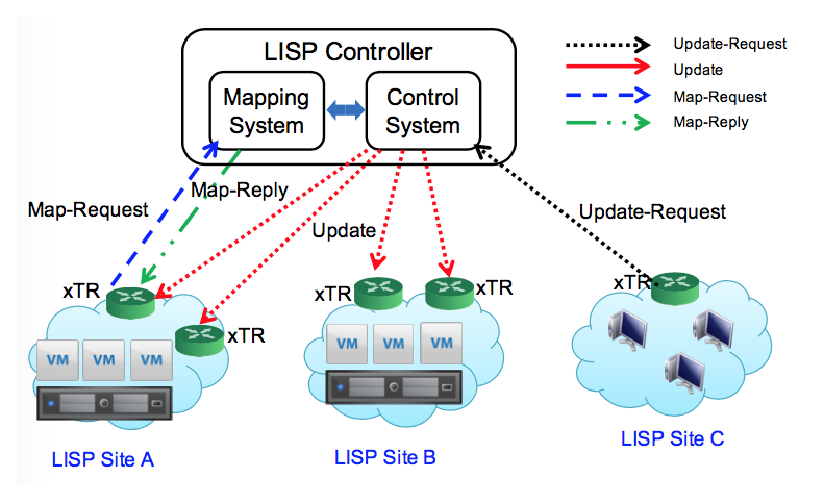
\includegraphics[width=\textwidth]{Pics/concept_of_LISP_controller.eps}
%	\caption{The concept of LISP controller (source:~\cite{han2016design})}
%	\label{concept_of_LISP_controller}
%\end{figure}
%%-< END FIGURE >--------------------------------------------------------------------
The LISP controller in Open Network Operating System (ONOS), which is an open source SDN OS for service providers~\cite{han2016design}, is one of South Bound Interfaces (SBI) for SDN controllers. The LISP controller in ONOS is proposed to address the OpenFlow issues, such as: scalability, performance, heterogeneity, interoperability with legacy networks and protocols. An open source SDN controller development project called OpenDaylight~\cite{OpenDaylight}, includes a sub-project, which is developing the LISP mapping system in SDN environments. The LISP controller centralizes LISP controls into a single entity. It supports LISP as an SDN SBI to work with other protocols such as OpenFlow, and provides APIs for LISP applications. % The concept of LISP controller is depicted in Fig.~\ref{concept_of_LISP_controller}. 
The LISP controller brings many benefits, such as: simplified management, a global view of LISP networks, short information convergence time, and easy development support of LISP based applications. 

%-< SUB SECTION >--------------------------------------------------------------------
\subsection{The LISP simulation gap}
\label{subsec:implementation_missing}
At the moment, LISP has some implementations for the different Operation Systems, either proprietary or open source. However, researchers prefer to test new features on simulations rather than real testbeds, because the simulation environment simplifies the studied problem and allows researchers to concentrate on the most critical issues~\cite{moller2011simulation}. So, simulation has a dominant capability over the other evaluation tools, when the researchers want to quickly test new features on a larger scale for different network scenarios. Among the recent network simulators, such as ns-2~\cite{breslau2000advances}, ns-3~\cite{henderson2008network}, OMNET++ and OPNET~\cite{chang1999network}, basic LISP features have already been added to OMNET++. However, it is not open source, which poses issues for the researchers to easily and flexibly conduct the simulations. In addition, ns-3 is more popular with the researchers than the others~\cite{rana2017implementation} and there was an open source project\footnote{Source code is available at~\cite{lionel2016}.} implementing the fundamental LISP on it in 2016. Whereas this project is based on ns-3.24 (the version at that moment), and it does not support features related to LISP mobility. Thus, we decide to leverage on this project, but first adapt to ns-3.27, and realize the extension of LISP mobility. Such contribution will be introduced in Chapter.~\ref{cha:ns-3}. 

\section{LISP mapping system evaluation}
\label{sec:mds}

%-< SUB SECTION >--------------------------------------------------------------------
\subsection{Current studies}
\label{subsec:mds_studies}
The performance of LISP Mapping System is evaluated in~\cite{lispCCR} and~\cite{coras2014performance} from different aspects. As the LISP Beta Network changed its mapping system from LISP+ALT to LISP-DDT on March \nth{14} 2012, the authors measure the delay of resolving mapping (the latency between sending the Map-Request and receiving the Map-Reply) during this transition period. They find the delay to get the mapping by using LISP+ALT is smaller and more stable than LISP-DDT. However, the manageability of the latter is better than the former, since by using LISP+ALT, % the Map-Requests normally need traverse the entire BGP overlay and 
maintaining the ALT causes many cumbersome configuration overhead especially as the network growing. Although using LISP-DDT slightly degrades the resolving performance, the delays remain small and the mapping system is able to cope with a significant growth of number of mappings. % The resolution delay is slightly various from the vantage points and the \acrshort{mr}s, but the European infrastructure is unreliable due to the loss of many queries.

%-< SUB SECTION >--------------------------------------------------------------------
\subsection{The incomplete puzzle of MDS evaluation}
\label{subsec:mds_missing}
The previous measurements of the \acrshort{mds} are mainly depended on the delay, including the different resolving latency that each \acrshort{mr} needs to use, and comparing which \acrshort{vp}s have longer delay to query the mappings. However, the authors have never taken look at the contents of mapping information, i.e., the type of mappings and locators etc.. In addition, there is no work to compare whether the consecutively received Map-Replies change over time. If yes, how they change? If there is any pattern? There are also no comparisons on whether the Map-Replies sent by the different \acrshort{mr}s for the same \acrshort{eid}s are identical. Neither for the Map-Replies received by the various \acrshort{vp}s. All these evaluations will be discussed in Chapter.~\ref{cha:mds_evaluation}.


\section{LISP network evolution}
\label{sec:evolution}
%%-< SUB SECTION >--------------------------------------------------------------------
%\subsection{Current studies}
%\label{subsec:evolution_studies}
After deploying LISP in LISP Beta Network from 2008, more and more participants joined to the development of LISP. % The LISP network is steady flourishing. 
Thus, Saucez et al.~\cite{lispCCR} look at how the LISP Beta network evolves. The authors observe that the number of LISP mapping was as low as 20 in January 2010, but it has consistently grown to reach 80 mappings in 2012. The number of LISP mappings is four times the initial number, which indicates that LISP network has a regular growth. Within two months of the second part of 2011, the number of negative mappings was doubled, i.e., from about 150 to about 300. The authors suppose that is due to a more fragmented EID-space. The paper also observes some malformed mappings, which belongs to the LISP mappings but have an empty RLOC set. However, this kind of mappings is never more than 0.5\% of the total number of mappings within one day. Further, the paper presents that from January 2010 to May 2012, the percentage of mappings using one or two RLOCs has increased. Moreover, there exist mappings with four RLOCs in 2012, whereas they were not present in January 2010.

%-< SUB SECTION >--------------------------------------------------------------------
\subsection{Updating LISP measurements}
\label{subsec:evolution_missing}
Previous works respectively evaluate the LISP network evolution in 2010 and 2012. However later, LISP mapping system is changed from \acrshort{lispalt} to \acrshort{lispddt} in 2012. Besides, as mentioned in Sec.~\ref{subsec:platform_lab}, LISP-Lab platform is open since 2015. It brings new LISP-sites over the world and interconnects with LISP Beta Network. Further, LISP Beta Network itself also updated their xTRs and changed its network architecture in 2016. Thus, the number of LISP mappings, the fragment of EID-space, the distributions of RLOCs are also changed over time. It is interesting to have a look at them in order to know how the LISP network evolved in recent years. This work will be described in Chapter.~\ref{cha:LISPViews}.

%-< SECTION >--------------------------------------------------------------------
\section{LISP interworking with legacy Internet}
\label{sec:interworking}

%%-< SUBSUB SECTION >--------------------------------------------------------------------
%\subsection{Impact on traffic between LISP-site and the legacy Internet}
%\label{subsec:interworking_impact}
% LISP has no impact on traffic to nowadays legacy Internet if neither source nor destination is LISP. However, it 
LISP has significant impact on the traffic between LISP-site and non-LISP-site. First, to support the interworking between LISP-site and the legacy Internet, the PxTRs should be set up. The configuration on \acrshort{pxtr} does not cause any special technical issue, but using \acrshort{pxtr} potentially causes path stretch between source and destination. It makes the packet exchange experience a larger delay and potentially leads to higher packet loss rate. Thus, placing the PxTR near the source/destination of traffic allows the communication between the non-LISP site and the LISP site to have the least path stretch (i.e., the least number of forwarding hops when compared to an optimal path between the sites)~\cite{rfc6832}. % Moreover, as PxTRs advertise in BGP the EID-prefixes that they are behalf of, if they are managed by different entities (i.e., they belong to different ASes), it is possible to cause MOAS (Multi-Origina AS) issues~\cite{rfc7834}.

When deploying the PxTRs in the experimental infrastructure, it is better to think about first where to deploy the PxTRs, since the placement in topology has a significant impact on the path stretch. Besides, as the number of PxTRs has a direct impact on the traffic load and the recovery success in case of the failure of a PxTR, we need consider how many PxTRs are needed. Further, we need to think if it is necessary that all the PxTRs advertise for the whole EID space, or it only needs that each of them just announces for the different segmented EID-prefixes.

%%-< SUB SECTION >--------------------------------------------------------------------
%\subsection{Current studies}
%\label{subsec:interworking_studies}
As more and more deployments of LISP, it becomes necessary that the LISP networks communicate with the legacy Internet. The evaluation of the interworking performance is presented in reference~\cite{coras2014performance}. It chooses 200 \acrshort{vp}s on the PlanetLab (a global research network that supports the development of new network services from 2003)~\cite{PlanetLab} located in North America, Asia and Europe by the order of diversity of number of \acrshort{vp}s. It also selects 116 EIDs, which have at least 1 corresponding RLOC in the mapping from the daily of LISPmon project~\cite{lispmon} published on May \nth{17} 2013. The experiment is conducted from November \nth{4} to \nth{7} 2013. The authors find that the interworking generally has a negative impact compared to not using LISP. The results show that there are 70\% of the EID-prefixes having at least 20\% of increase in the delay (i.e., \acrfull{rtt}). One \acrshort{pxtr} behaves the worst, with 95\% of the EID-prefixes using it suffering from a delay increase. Based on BGP, the selection of \acrshort{pitr}s is driven by the economical relationship between autonomous systems, instead of their geographical positions. As a result, even if the LISP Beta Network has 9 available \acrshort{pxtr}s at the moment, only 4 are used in the experiment. Further, most \acrshort{vp}s use \acrshort{pxtr}s in Asia although they are located in Europe or America. The most popular \acrshort{pxtr} is selected 79\% of the time.

%-< SUB SECTION >--------------------------------------------------------------------
\subsection{PxTRs evaluation: an incomplete picture}
\label{subsec:interworking_missing}
The only evaluation of PxTR used for the interworking between LISP and legacy Internet was conducted in 2013. At that time, the unique LISP platform was the LISP Beta Network. Thus, the measurement was only based on its PxTRs and the \acrshort{vp}s on the research network PlanetLab. After the addition of the LISP-Lab platform in 2015, there is no evaluation about the PxTR anymore. We do not know the recent performance of PxTR on LISP Beta Network and we have no knowledge about if the PxTR of LISP-Lab functions well. Further, the previous assessment was conducted within an experimental/research environment, there is no experience about the interworking performance with real sites, especially for the most popular websites on the world. In the Chapter.~\ref{cha:pxtr}, we will explore all these issues of LISP interworking performance.

\section{LISP mobility}
\label{sec:mobility}

%%-< SUB SECTION >--------------------------------------------------------------------
%\subsection{Current studies}
%\label{subsec:mobility_studies}
% \yue{Support for Network-based User Mobility with LISP}
To support IP mobility, the conventional LISP could be adopted. The first mobility-compatible LISP extension is LISP-MN~\cite{mn00}\cite{natal2013lisp}. LISP-MN is an end-host based IP mobility protocol which requires updating the software of the mobile terminal. In other words, the end-host that uses LISP-MN can be regarded as a small LISP-site.

The main drawbacks of LISP-MN are the double encapsulation that may happen and the need to modify software in end-host. Double encapsulation increases mapping latency, overhead and MTU issues. The modification at end-host hinders the deployment of LISP-MN. To overcome these drawbacks, lots of research efforts have been made by the LISP community.

The performance of LISP-MN is investigated by M. Menth and et al.~\cite{menth2010improvements}. The authors illustrate the performance degradation due to double encapsulation and the triangle route problem under some conditions. They also propose mechanisms such as location-aware LISP mobility node, local mapping systems to improve the performance of LISP-MN. A simple model that help analyze the handoff procedure in IP mobility is proposed by~\cite{phoomikiattisak2016control}. Besides LISP-MN, the proposed model can be also used for the handoff analysis for other IP mobility protocols such as MIPv6. 

To avoid the modification to end-host required in LISP-MN, a network-based and LISP-based IP mobility protocol: LISP-ROAM is proposed in~\cite{galvani2014lisp}. Their solution is that the network assigns the same IP address regardless of their network attachment point under the cooperation between some additional/modified network components (DHCP servers, authentication services, LISP xTR and servers). The authors implement LISP-ROAM on top of LISPmob and give an experimental evaluation of the performance of LISP-ROAM. As an effort to avoid double encapsulation in LISP-MN, LISP-NEMO is proposed in~\cite{wu2014nemo}. The basic idea of LISP-NEMO originates from NEMO~\cite{jeon2010network}. It introduces a new network element called mobile router (MR) that manages and represents the mobile network. To mitigate the problems in LISP-NEMO and LISP-ROAM, LISP-HNM is proposed in~\cite{tang2017lisp}. The authors introduce an access register protocol and an active
notification scheme to conventional LISP so that the latter can support both end-host and network mobility.

The packet loss due to IP mobility is also a concern. To reduce the packet loss, Isah et al.~\cite{isah2017towards} propose an improvement to LISP-MN. The basic idea is that those packets generated during handover procedure are buffered to severs close to the MN’s new location and forwarding them to the MN on handover completion.

% Essentially conceived for mobile equipment, LISPmob could also be installed in the VM; there would be, however, a problem with most current hypervisors that impose the VM external address to be in the same subnet before and upon migration, which practically limits the LISPmob usability only to situations where source and destination networks are either LISP sites themselves, or layer-2 over WAN solutions. In the first case, a double encapsulation is needed, which could increase mapping latency, overhead and MTU issues. There may also be scalability issues with a high VM number.

%-< SUB SECTION >--------------------------------------------------------------------
\subsection{Open issue in LISP mobility}
\label{subsec:mobility_missing}
To achieve the seamless handover, LISP can be implemented on the border router or directly on the host to support the mobility. However, these proposals are only limited at the theoretical level. There are no experimental results showing which solution is better based on some metrics, such as: the smaller handover delay or the less packet loss. No evaluations respectively compare the advantages and the disadvantages of each solution. What's more, no matter which solution is adopted to conduct the mobility, SMR and Map-Versioning are the candidates to say to the remote ITR to update its mapping cache. Thus, it is interesting to make a comparison between these two mechanisms, for example modeling the overhead traffic according to the number of \acrshort{mn}s and \acrshort{cn}s of each mechanism. Chapter.~\ref{cha:ns-3} will analyze those scenarios.


%-< SECTION >--------------------------------------------------------------------
\section{Troubleshooting issues}
\label{sec:troubleshooting}
A big issue in the LISP experimentation is the difficulty of troubleshooting. The most frequent used troubleshooting tool is \emph{traceroute}, but it can not provide the exact path that the packets pass between the xTRs or PxTRs. The experimenters only know how many hops between them. When the host traceroutes a destination, it uses each EID as the source/destination IP address. However, when the packets pass to the \acrshort{itr}, it encapsulates the packets, so the following routers think that the \acrshort{itr} is the source of the packet and will give back the ICMP message to the \acrshort{itr}. In this way, the host, which is the real source receives no response. Until the packets reach to \acrshort{etr} or \acrshort{petr}, they decapsulate the packets to know the real source from the inner header and answer to the EID of host.

%-< FIGURE >--------------------------------------------------------------------
\begin{figure}[!t]
	\centering
	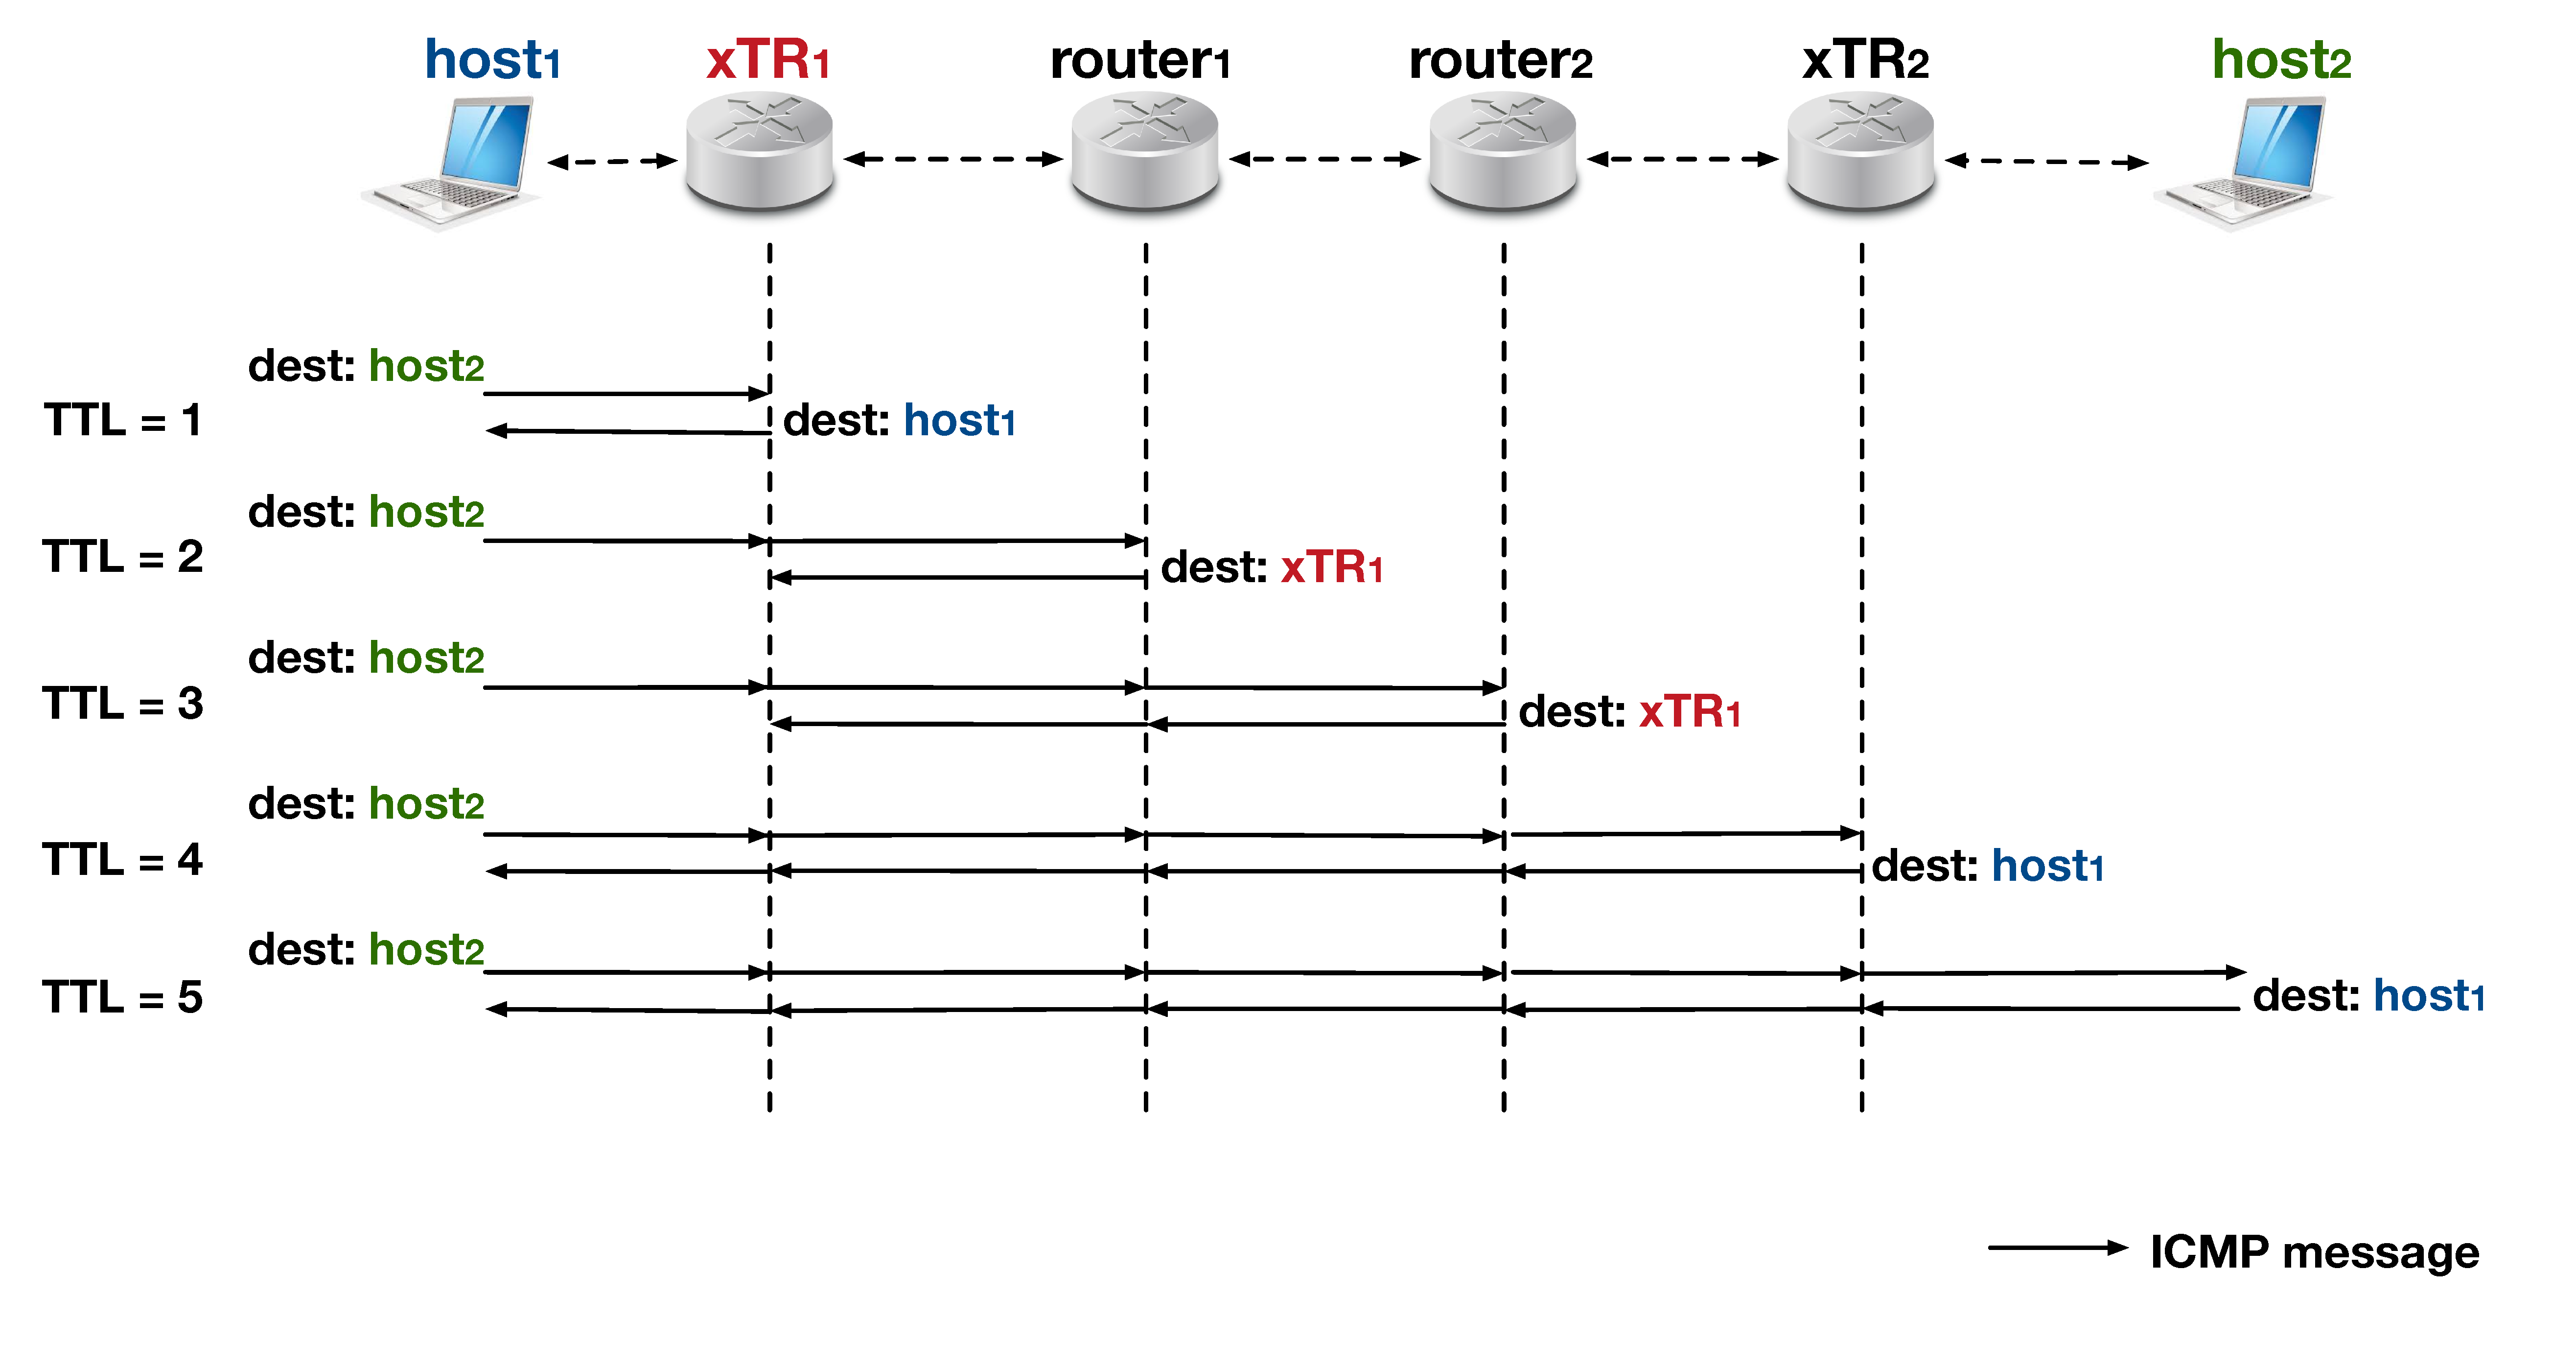
\includegraphics[width=\textwidth]{Pics/LISP_traceroute.eps}
	\caption{Illustration of LISP troubleshooting}
	\label{Illustration_LISP_troubleshooting}
\end{figure}
%-< END FIGURE >--------------------------------------------------------------------
An example of LISP troubleshooting is shown in Fig.~\ref{Illustration_LISP_troubleshooting}. When $host_1$ traceroutes $host_2$, $host_1$ puts its own EID and the one of $host_2$ respectively as source and destination address. The first UDP message with TTL (time-to-live)=1 expires at $xTR_1$, then it sends back the ICMP Time Exceeded message to $host_1$. Thus, the $host_1$ knows that its next hop is $xTR_1$. However, when $xTR_1$ receives the UDP message with TTL=2, it decreases the TTL value, and encapsulates the UDP message with its own RLOC as source address and forwards to the next hop $router_1$. Since the UDP message that the $router_1$ receives showing $xTR_1$ is the source instead of $host_1$, the $router_1$ drops the packets and replies back to $xTR_1$. In this way, the $host_1$ cannot receive any ICMP Time Exceeded messages until the $xTR_2$ is tracerouted. When the $xTR_2$ receives the UDP message, it decapsulates the packets and finds that the real traceroute sender is $host_1$. Thus the $xTR_2$ replies to $host_1$. Same to $host_2$, the received UDP message shows that $host_1$ is the traceroute origin and itself is the destination, so it returns an ICMP Port Unreachable message $host_1$. 

To the conventional Internet topology, \emph{traceroute} uses the returned ICMP Time Exceeded messages to build a list of routers that packets traverse until the destination is reached. However, % due to the troubleshooting problem LISP facing to, 
the list of routers between xTRs is hidden to the traceroute sender. It can only know how many hops it needs to arrive the ETR. Thus, when there is a problem in the LISP network, it is hard for the operators to pinpoint the reason as they have only a partial view of the network. The experimenters can leverage on the LISP Cache/Database or querying the \acrshort{mr}s to observe the potential problem in the network, but the knowledge remains limited. 

This issue brings inconveniences to our experiment, which will be discussed in Chapter~\ref{cha:pxtr}. In that experiment, we can only find how many hops there are between our \acrshort{vp}s and the PxTRs, but are not able to specify the exact routing paths.

%-< SUB SECTION >--------------------------------------------------------------------
\section{Other LISP Related studies}
\label{subsec:other_studies}
LISP is relatively young and there are many other aspects needed to be taken into consideration, such as: the caching, the LISP security, the MTU issue, and so on. As they are important and necessary to LISP, we list them here. However, since they are not related to this dissertation, they will not be discussed in the following chapters.

\subsection{LISP Cache performance}
\label{subsec:cache}

%\subsubsection{Current studies}
%\label{subsubsec:cache_studies}
A thorough analysis of LISP Cache is presented in~\cite{lispCacheCost},~\cite{lispCacheDive} and~\cite{kim2013caching}. Their work complement and validate each other. The papers %analyzes two 24-h traces of a large European ISP and shows 
show that although the cache timeout can be reduced % from initial 24-h to 
as small as 60s, the LISP cache maintains a very high efficiency, with more than 99\% hit-ratio. As a result, % the cache highly reduces the size, and 
the traffic volume overhead introduced by both the traffic encapsulation and the control traffic to request missing mappings is limited to 6\%. Around 70\% of cache miss is generated by UDP protocol regardless the port number. The authors argue that is mainly caused by P2P applications or other distributed applications generating the same spread traffic pattern. They also compare the original LISP specification, called vanilla LISP with the symmetric LISP model, proposed by Saucez et al.~\cite{lispCacheDive}, and show that the later model provides higher security. Besides, they evaluate the relationship between the size of cache and the number of users. It shows that when the number of users is increased to three times, the size of cache only doubles. It means that the average size of the LISP Cache has not a linear relationship with the number of hosts.

%\subsubsection{Missing work}
%\label{subsubsec:cache_missing}
As querying the mapping information to the \acrshort{mds} largely increases packet transmission delay, to store the necessary mappings in the LISP Cache can significantly alleviate it. However, as limited capacity of LISP Cache and dynamic changes of mapping information, it still requires smart algorithms to determine which mappings should be reserved or removed for better performance, especially when there are many expired mappings caused by mobility~\cite{feng2017locator}.


\subsection{LISP security}
\label{subsec:security}

%%-< SUBSUB SECTION >--------------------------------------------------------------------
%\subsubsection{LISP security impact}
%\label{subsubsec:security_impact}
As LISP is born to address the scalability issues of Internet, it is not designed with security in mind. The possible security threats that LISP faces are given in~\cite{rfc7835}. Although after the authentication, the \acrshort{ms}es only accept the registrations from trusted ETRs, the mapping system can still be attacked. For example, compromised ETRs may de-aggregate their EID-prefixes in order to register more EID-prefixes than necessary to their \acrshort{ms}es, and this causes the ITRs to send overwhelmed Map-Requests to the mapping system. The compromised ETRs may also overclaim the prefix they own in order to influence the route followed by Map-Requests for EIDs outside the scope of their legitimate EID-prefix. Besides, the Map-Register stage is vulnerable to masquerading and content poisoning attacks, for example: the ETRs register the fake mapping information to the \acrshort{ms}es~\cite{aiash2013securing}~\cite{montero2013securing}~\cite{aiash2013novel}. By sending the Map-Requests at a high rate can overload the nodes in the MDS and cause the flood of Map-Replies as well. Some bits in the LISP control plane messages also have some security issues, for example: the Locator-Status-Bits can cause a DoS (Denial-of-Service), a replay, a packet manipulation, or a packet interception and suppression attack; the Map-Version number can mount a DoS, an amplification, or a spoofing attack; the routing locator reachability is able to mount a packet manipulation and an amplification attack.

A set of security mechanisms (LISP-SEC) that provides authentication, integrity and anti-replay protection for LISP are introduced by Maino et al.~\cite{maino2017lisp}. A number of vulnerabilities should be considered before deploying LISP in large scale~\cite{raheem2013supporting}.

%\subsubsection{LISP security proposal}
%\label{subsubsec:security_proposal}
The paper of Aiash et al.~\cite{aiash2013novel} analyses the security and functionality of the LISP mapping procedure using a formal methods approach based on Casper/FDR tool. The authors point out several security issues in the protocol such as the lack of data confidentiality and mutual authentication. The reference~\cite{aiash2013securing} figures out that the Map-Registration stage is vulnerable to masquerading and content poisoning attacks. Therefore, it presents a new security method for protecting the LISP Registration stage. The proposed method uses the ID-Based Cryptography (IBC), which allows the \acrshort{mds} to authenticate the source of the data. 

%-< SUBSUB SECTION >--------------------------------------------------------------------
\subsection{The Maximum Transmission Unit (MTU) issue}
\label{subsubsec:mtu}
LISP encapsulation adds 36 bytes for IPv4 (i.e., 20 bytes of outer header + 8 bytes of UDP header + 8 bytes of LISP header) and 56 bytes for IPv6 (i.e., 40 bytes of outer header + 8 bytes of UDP header + 8 bytes of LISP header) to the original packet size. As with other protocols that encapsulate or tunnel traffic (e.g., IP Security (IPsec)~\cite{thayer1998rfc} and generic routing encapsulation (GRE)~\cite{farinacci2000generic}), it is possible that the resultant encapsulated packet would exceed the MTU somewhere along the transit path. LISP provides both stateful and stateless mechanisms for handling potential MTU issues~\cite{CiscoLISPQA}, with the main goals being 
\begin{enumerate*}[label=(\roman*)]
	\item preventing packets from being dropped, and
	\item preventing the need for ETRs to perform packet reassembly prior to LISP de-encapsulation. 
\end{enumerate*}

Based on real Internet experiments, \cite{lispCacheCost} and \cite{kim2013caching} show that although the encapsulation overhead is not negligible, it is very limited (in the order of few percentage points of the total traffic volume). In addition, no major issue due to the MTU is observed on the LISP Beta Network.


 % Related work
%*******************************************************************************
%****************************** Third Chapter *********************************
%*******************************************************************************

\chapter{Evaluation of LISP mapping system}
\label{cha:mds_evaluation}

% **************************** Define Graphics Path **************************
\ifpdf
    \graphicspath{{Chapter4/Pics/Raster/}{Chapter4/Pics/PDF/}{Chapter4/}}
\else
    \graphicspath{{Chapter4/Pics/Vector/}{Chapter4/}}
\fi

%-< ABSTRACT >--------------------------------------------------------------------

%-< ABSTRACT >--------------------------------------------------------------------

\section{Introduction}
\label{sec:mds_introduction}

%In the LISP architecture, the mapping between RLOCs and EIDs is the cornerstone and a deep study on the performance of LISP mapping system is essential. 
As presented in Chapter~\ref{cha:lisp_overview}, to retrieve the routing information (RLOCs) for EIDs, LISP relies on a pull model by explicitly querying the \acrfull{mds}. The performance of the mapping system is of paramount importance for LISP. Thus, we leverage on \emph{LISP Beta Network}~\cite{lispbeta}, to conduct measurement campaigns about the mapping system. Such a worldwide real playground has been used to assess the state of LISP deployment and evolution over the years~\cite{lispCCR}. Yet, to our best knowledge, nobody at the moment has evaluated the mapping system from the following two standpoints: Stability and Consistency. We thus propose a much deeper study and a more thorough evaluation, focusing on the exploration of all the mapping systems on LISP Beta Network through active LIG (LISP Internet Groper~\cite{rfc6835}) measurement. The temporal comparison shows that the mapping system is quite stable over time and the crosswise comparison indicates that the mapping system is consistent between network entities. However, some instability and inconsistency cases are also identified through evaluation, which indicates that the mapping system can be improved. Hence, besides proposing a brand new taxonomy in order to classify them, we carry out an in-depth investigation of such cases to provide hints on how to improve the performance of LISP.

The remainder of this chapter is organized as follows. Sec.~\ref{sec:mds_methodology} presents an overview of the experiment campaigns and introduces the metrics that we use to evaluate the performance of mapping system. Sec.~\ref{sec:mds_stability} and Sec.~\ref{sec:mds_consistency} respectively describe the mapping system stability and consistency results in details, as well as the instability and inconsistency cases by using the proposed taxonomy, and investigate in depth the causes from different viewpoints. Finally, Sec.~\ref{sec:mds_conclusion} provides some findings in other scopes and concludes this chapter.

%-< SECTION >--------------------------------------------------------------------
\section{Methodology}
\label{sec:mds_methodology}
In order to collect data to carry out our analysis, several measurements campaigns have been performed. Hereafter we provide an overview on the measurements and the metrics used in our evaluation.

%-< SUB SECTION >--------------------------------------------------------------------
\subsection{Measurements Overview}
\label{sec:mds_overview}
% \begin{itemize}[noitemsep,topsep=0pt]
%     \item The experiments lasted two weeks, from July 2\textsuperscript{nd} to 18\textsuperscript{th} 2013. 
%     \item From a set of different vantage points (VPs).
%     \item Send the Map-Request to all the MRs of the LISP Beta Network by LIG.
%     \item Interval is 30 minutes.
% \end{itemize}
To obtain a comprehensive and in-depth evaluation of LISP Beta Network Performance, we conducted experiments using LIG (LISP Internet Groper~\cite{rfc6835}, see Sec.~\ref{subsec:implementation_lig} for the details). When LIG is launched, a \emph{Map-Request} is sent for a destination IP address, and the returned \emph{Map-Reply} is then stored for further analysis. It exists three possible types of outcome: 
\begin{inparaenum}[(i)]
	\item \emph{LISP Map-Reply}, where the reply contains mapping
	information to reach the LISP-enabled sites;
	\item \emph{Negative Map-Reply}, where the reply states that the requested IP address belongs to a prefix of a non-LISP site;
	\item \emph{No Map-Reply}, where no answer is received within some
amount of time.
\end{inparaenum}
A query is considered to be successful if either a LISP Map-Reply or a Negative Map-Reply is received. While a query is considered to be failed if no reply is received within 5 seconds. 

The experiments are conducted from July 2\textsuperscript{nd} to 18\textsuperscript{th} 2013. From a set of different vantage points (VPs), sending \emph{Map-Request} messages to all the Map-Resolvers of the LISP Beta Network, for all selected destination IP addresses every 30 minutes. The set of VPs was composed by part of academic networks, commercial Internet, PlanetLab and spread across Europe and USA. The destination IP addresses consisted of the first address within each prefix derived from the LISPmon project~\cite{lispmon} regardless of the type (i.e., the EID-prefixes or regular prefixes). During this measurement campaign, 5 VPs and 13 MRs/MSes were available and 613 prefixes were queried at each round. 

We analyzed the Map-Replies associated with EIDs instead of all regular IP addresses. In the remainder, we use the term \emph{experiment round} to
identify a complete \emph{Map-Request}/\emph{Map-Reply} exchange by LIG for all the selected destinations to all the available MRs over all existing VPs. Although No Map-Reply occasionally appears in some experiment rounds, we just focus on LISP Map-Reply and Negative Map-Reply to conduct the analysis. \footnote{We use \emph{"simultaneously"} or \emph{"at the same
time"} as synonym of \emph{"at a same experiment round"}.}


%-< SUB SECTION >--------------------------------------------------------------------
\subsection{Metrics}
\label{mds_metrics}
% Metrics are used to evaluate in this section:
% \begin{itemize}[noitemsep,topsep=0pt]
%     \item Definition of \textit{stability}. 
%     \item Definition of \textit{consistency} by MR.
%     \item Definition of \textit{consistency} by VP.
% \end{itemize}
As indicated in Sec.~\ref{sec:control_plane}, the LISP Control plane is in charge of offering the mapping information that consists of an EID-prefix associated with a list of \emph{<$RLOC, Priority, Weight$>} tuples. Theoretically, unless configuration has changed, if the same EID-prefix is queried, Map-Replies should always contain the same mapping information, no matter from which VP the query is sent, and no matter which MR is queried. During our measurements, however, we found that the Map-Replies are not always identical as they are supposed to be. The reasons causing the Map-Reply changes are summarized in Table~\ref{tab:List_of_possible_changes}. 

%-< TABLE >--------------------------------------------------------------------
\begin{table}[!t]
	\centering
	\caption{Map-Reply Differences}
	\label{tab:List_of_possible_changes}{
	\resizebox{0.8\textwidth}{!}{%
		\begin{tabular}{@{}c|c@{}}
			\hline\hline
            Category                    & Mismatch                              \\
            \hline
			Map-Reply Type              & Negative Map-Reply and LISP Map-Reply \\ \hline
			\multirow{5}{*}{RLOC set}   & RLOC number     \\ 
			                            & RLOC address    \\ 
			                            & RLOC priority   \\
			                            & RLOC weight      \\ 
			                            & RLOC state      \\ 
			                            \hline \hline                 
		\end{tabular}
	}}
\end{table}
%-< END TABLE >--------------------------------------------------------------------


The Map-Reply differences can be classified into two broad categories: the first is a difference in terms of \emph{Map-Reply Type}, which means that a mix of Negative Map-Reply and LISP Map-Reply occurs; the other type of difference is in the \emph{RLOC set}, which means that at least one of the attributes associated with RLOC set is different. More specifically, \emph{RLOC number} indicates a difference in the number of RLOC tuples received in the Map-Reply. The others are differences in a RLOC tuple, which consists of RLOC address, RLOC priority, and RLOC weight (presented in Sec.~\ref{sec:control_plane}).\footnote{The terms \emph{RLOC address} and \emph{RLOC} are used interchangeably in this chapter.} The RLOC state is derived from the \emph{R-bit} in Map-Reply message, which is set when the sender of a Map-Reply has a route to the RLOC, meaning that from its viewpoint the RLOC is up and running.  If at least one of the six parameters shown in Table~\ref{tab:List_of_possible_changes} conveyed in a Map-Reply is different from the previous one (over time) or the others (between different VPs or MRs) at the same experiment round, the Map-Reply is marked as different. Based on the criteria of the Map-Reply difference, we propose two metrics to evaluate in more details the performance of the LISP mapping system:
\begin{inparaenum}[(i)]
	\item \emph{Stability} and 
	\item \emph{Consistency}. 
\end{inparaenum}

A mapping is considered to exhibit \textit{stability} if the Map-Replies for one specific EID obtained from one MR observed at a given VP (briefly denoted as a tuple {<$EID, MR, VP$>}), over time, are identical. A classification taxonomy for unstable cases is proposed later in Sec.~\ref{sec:mds_stability}. 

A mapping exhibits \textit{consistency} if: $i)$ Map-Replies for a specific EID from all MRs observed at a given VP (denoted as a group {<$ EID, *, VP $>}) are identical at the same time (this kind of consistency is referred as \emph{Consistency by MR}); $ii)$ Map-Replies for a specific EID-MR pair in all VPs (denoted as a pair {<$ EID, MR, * $>}) are identical at the same time (referred as \emph{Consistency by VP}). A classification taxonomy for non-consistent cases is proposed later in Sec.~\ref{sec:mds_consistency}. 


%-< SECTION >--------------------------------------------------------------------
\section{Mapping System Stability Evaluation}
\label{sec:mds_stability}
% \begin{itemize}[noitemsep,topsep=0pt]
%     \item 91.49\% of observations are stable.
%     \item For the instability, we classify into 4 cases: 
%     \begin{itemize}[noitemsep,topsep=0pt]
%         \item New Deployment is 72.36\%. 
%         \item Reconfiguration is 20.41\%.
%         \item Mobility is 0\%.
%         \item Statistical outliers is 7.23\%.
%     \end{itemize}
%     \item Explain CDF of dissimilarity.
% \end{itemize}

In this section, we study the stability of the mapping system over time. More precisely, we consider that an EID is \emph{stable} if all mappings retrieved for this EID are identical. If it is not the case, we say there is \emph{instability}.

Overall, when we consider the whole dataset, 91.49\% of observations are stable, which indicates that over the full set of observations, changes are infrequent and the MDS is stable. When the stability is considered on a per vantage point basis, we observe, as shown in Fig.~\ref{fig:Percentage_stability_5VP_time}, that the stability is independent of the vantage point since no significant deviation from the overall average can be observed (dashed line in Fig.~\ref{fig:Percentage_stability_5VP_time}). Nevertheless, while these results demonstrate that the mapping system is generally stable, in the following of this section, we investigate the reason why about 8.51\% of the observations exhibit instability.

%-< FIGURE >--------------------------------------------------------------------
\begin{figure}[t]
    \centering
	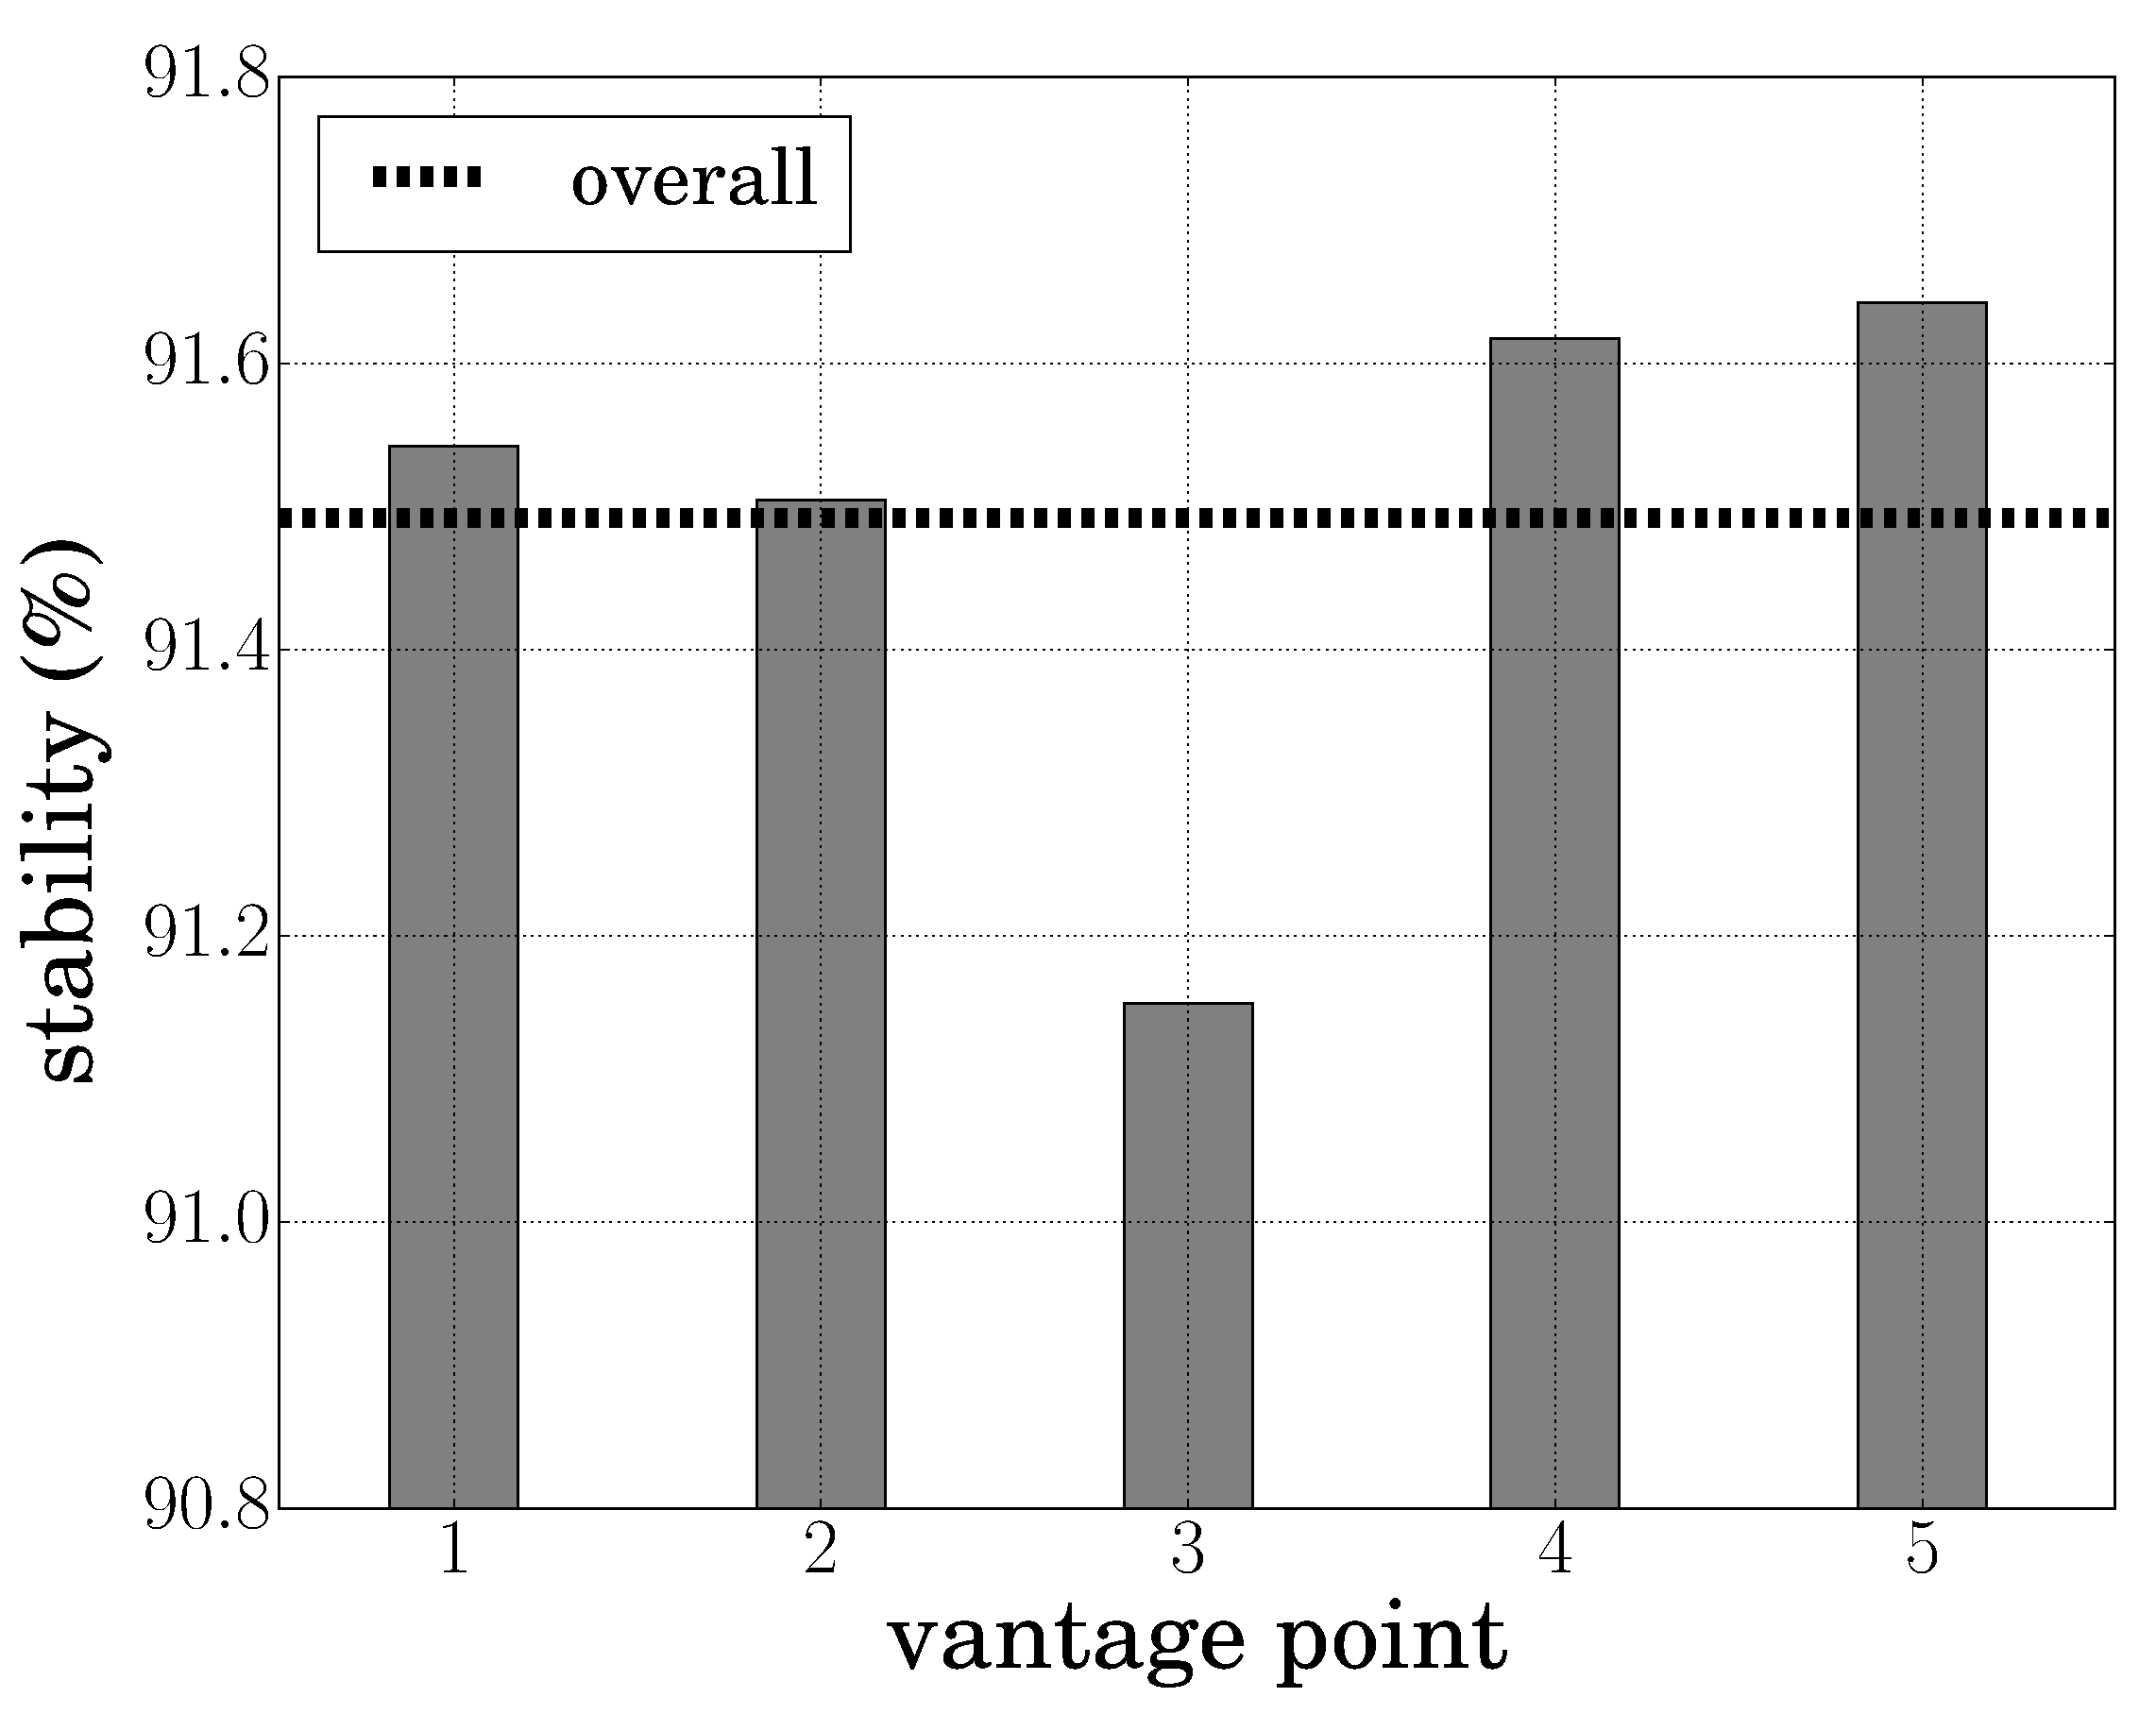
\includegraphics[width=0.7\textwidth]{Pics/Percentage_stability_5VP_time.eps}
	\caption{Overall percentage of stability observed at five different VPs.}
	\label{fig:Percentage_stability_5VP_time}
\end{figure}
%-< END FIGURE >-----------------------------------------------------------------

%-< FIGURE >--------------------------------------------------------------------
\begin{figure}[t]
	\centering
	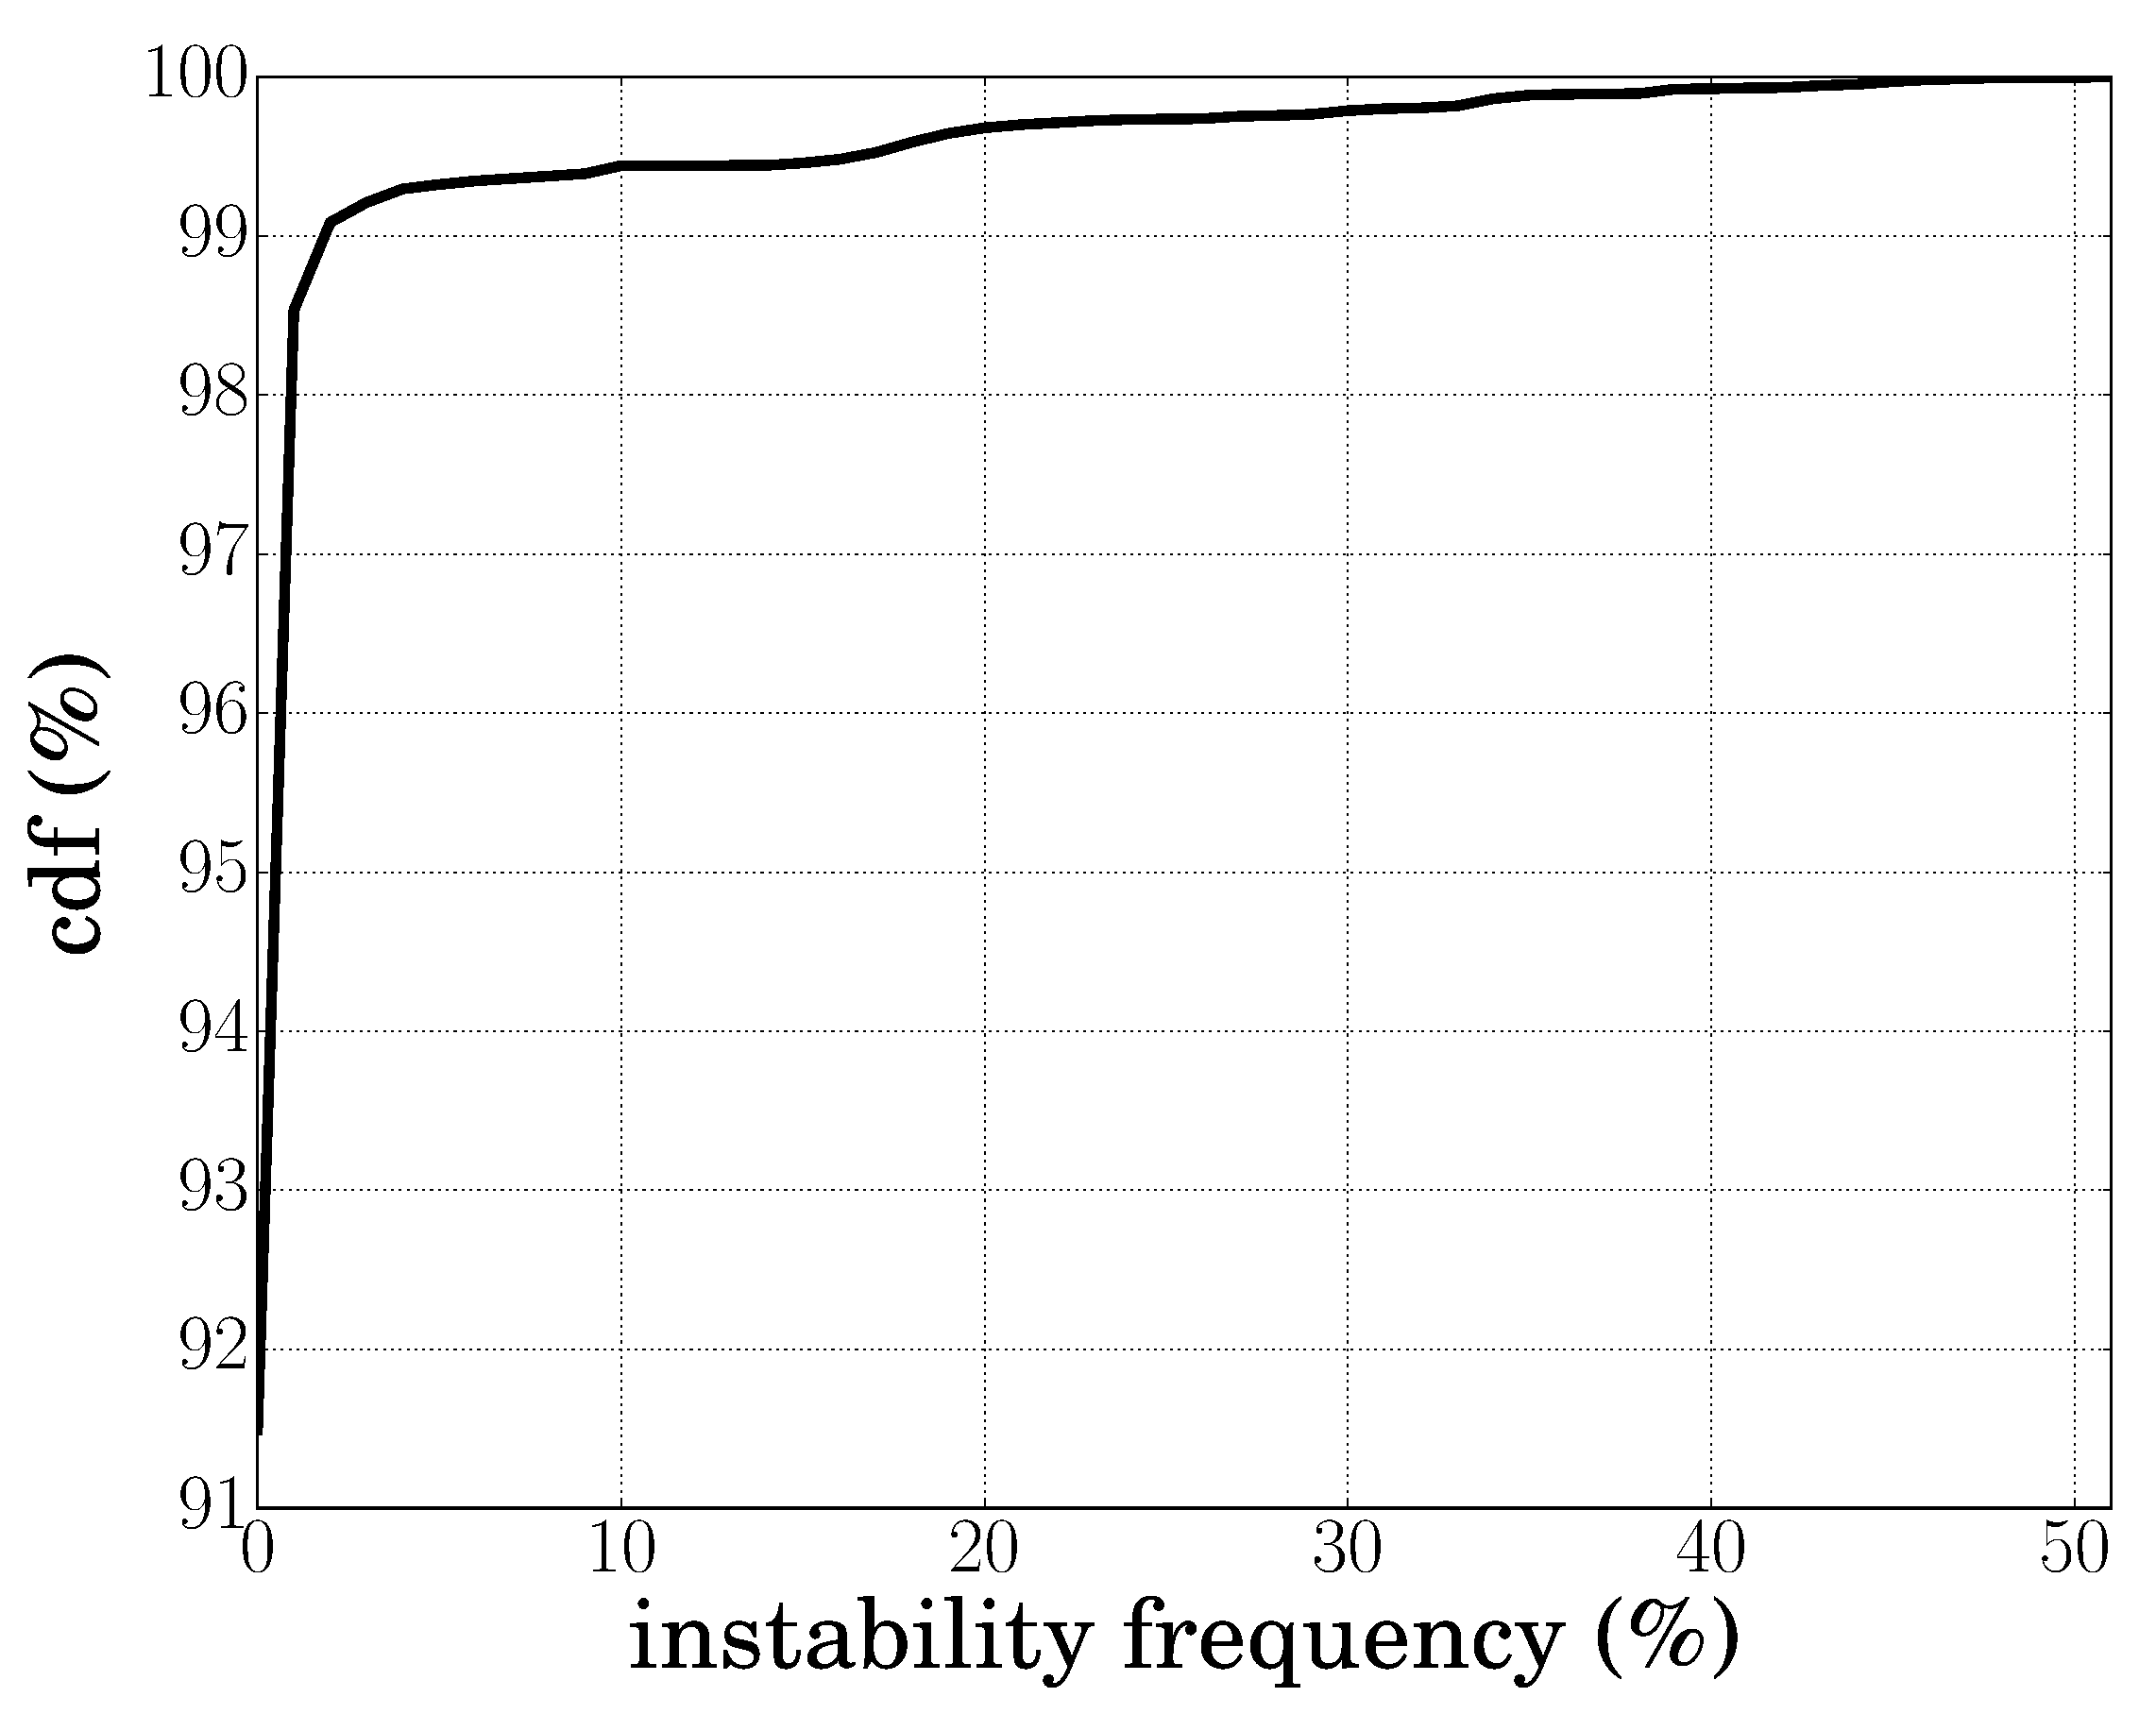
\includegraphics[width=0.7\textwidth]{Pics/cdf_instability_occur.eps}
	\caption{CDF of instability frequency. X-axis is instability frequency, indicating the ratio of instability occurrence number for one <$EID, MR, VP$> tuple over total experiment number.}
	\label{fig:cdf_instability_occur}
\end{figure}
%-< END FIGURE >-----------------------------------------------------------------


%-< FIGURE >--------------------------------------------------------------------
\begin{figure}[t]
	\centering
    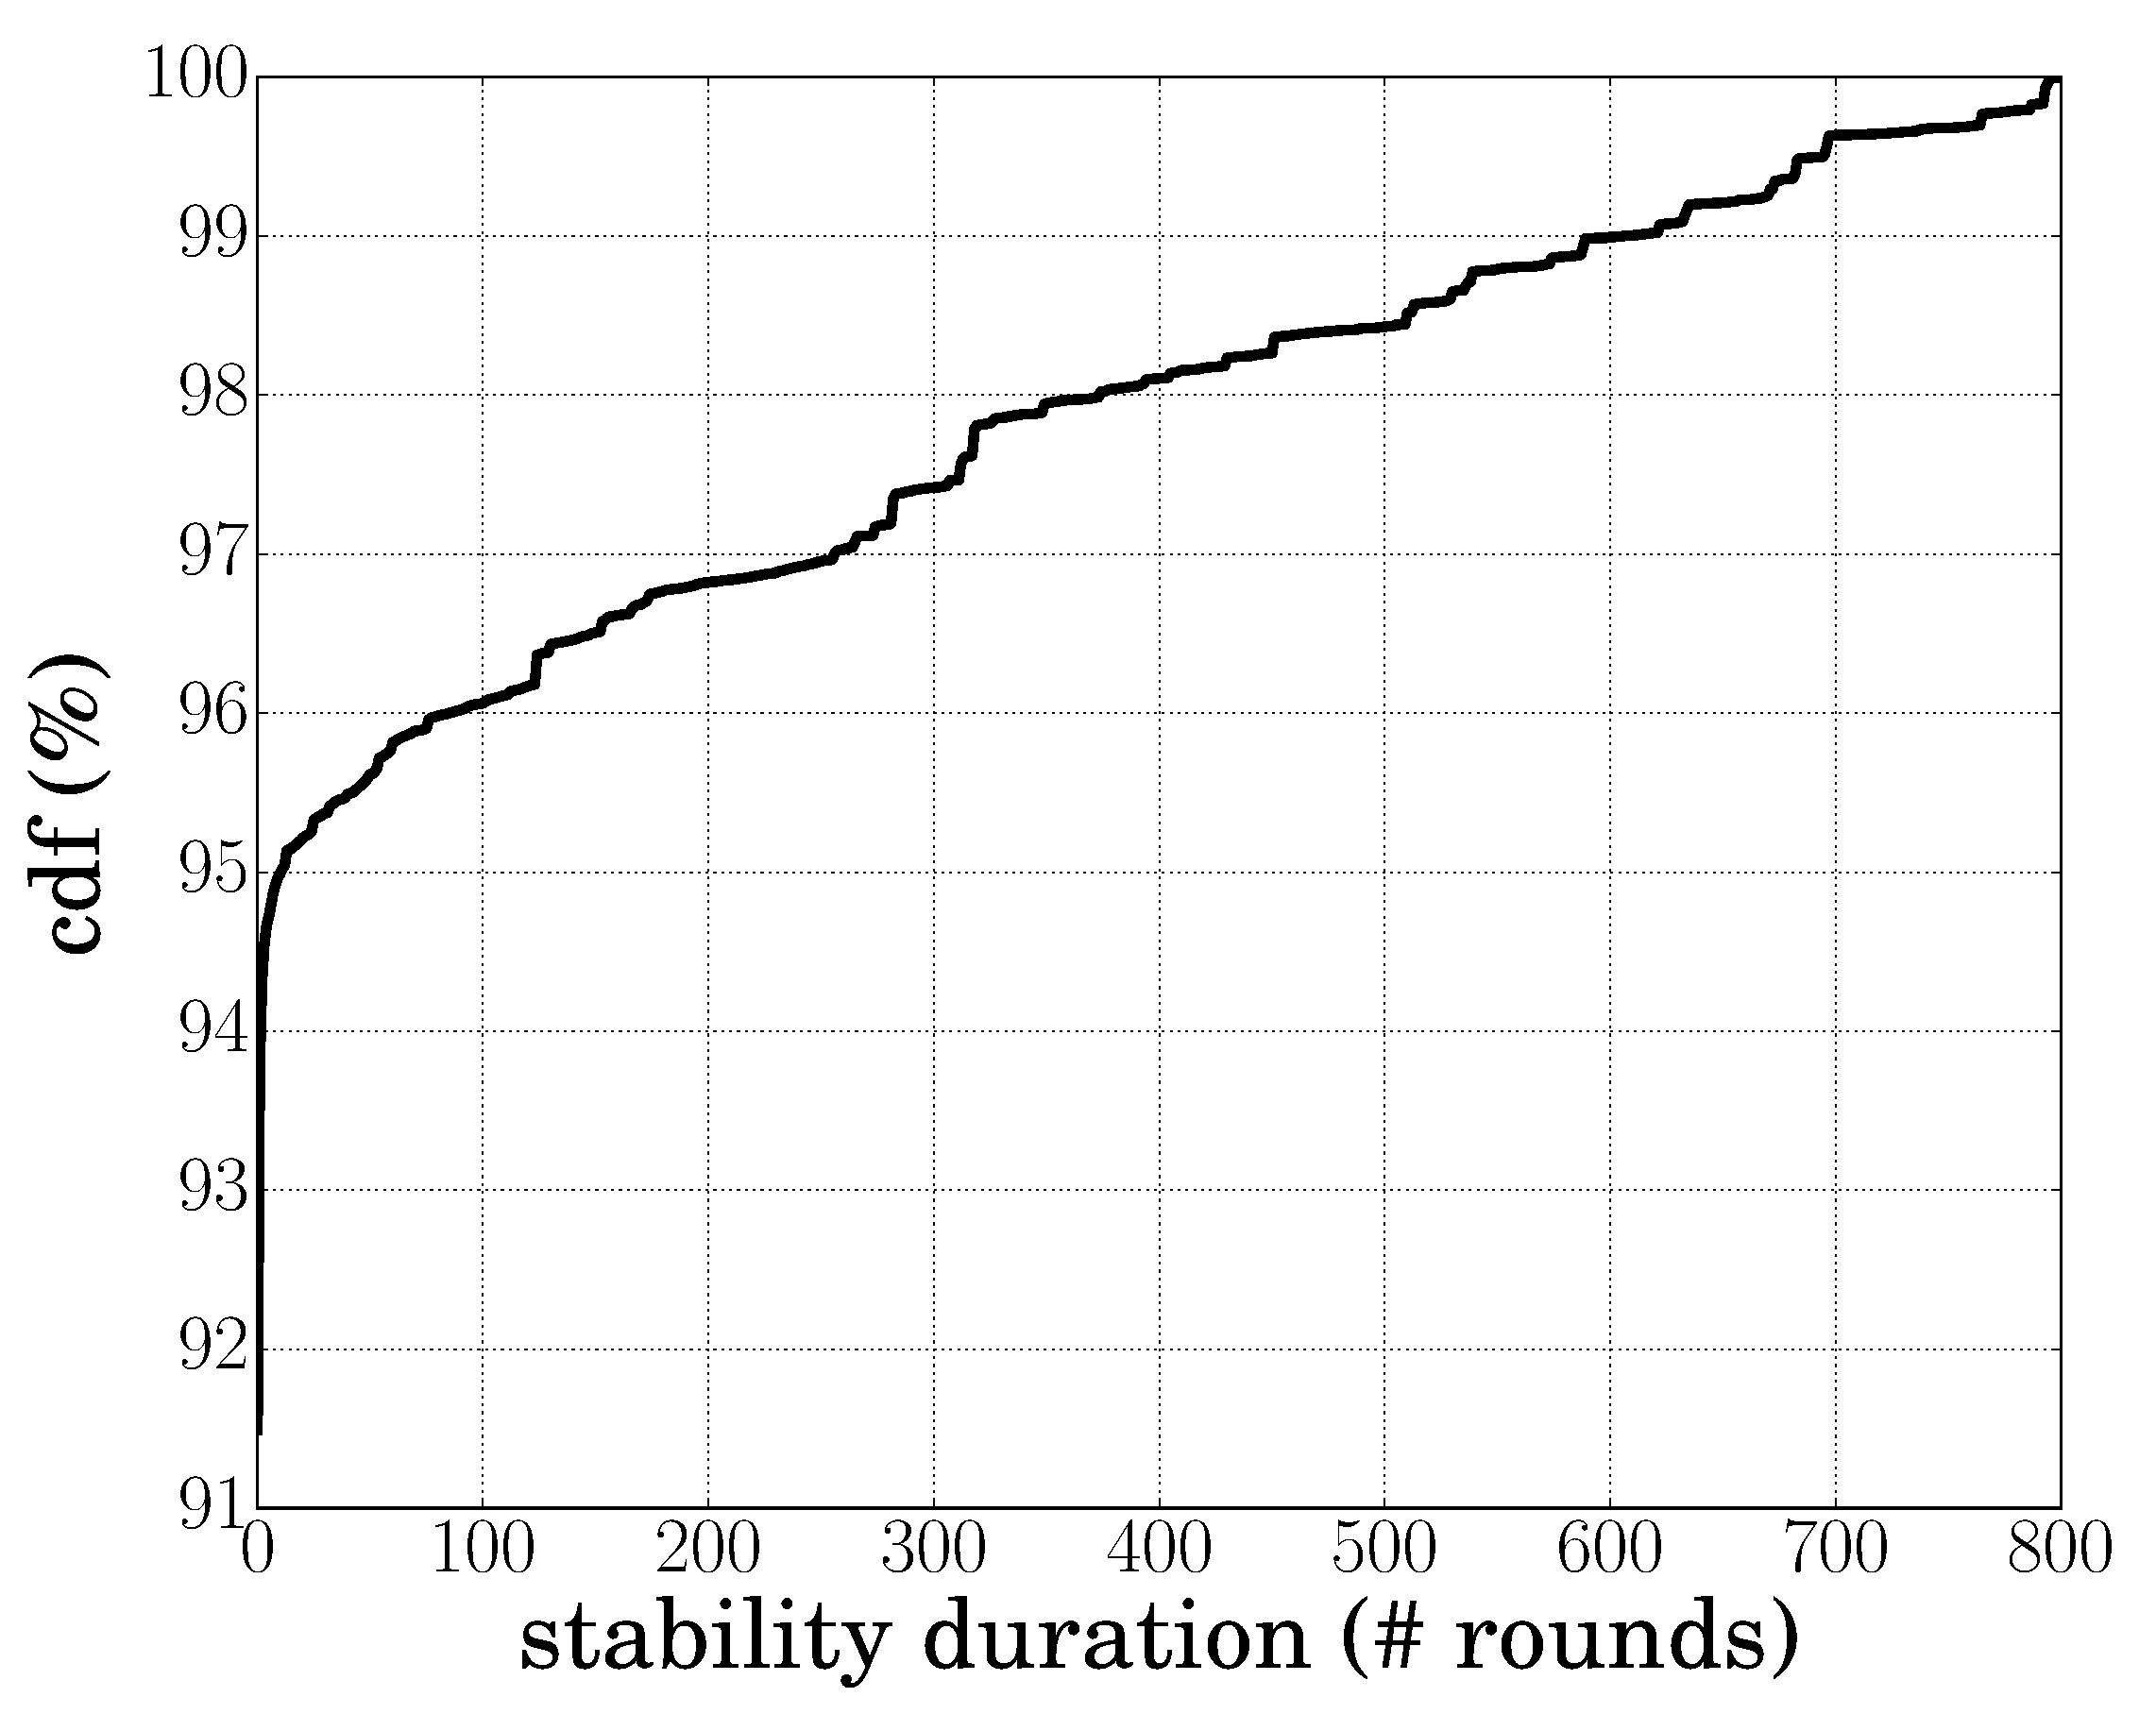
\includegraphics[width=0.7\textwidth]{Pics/cdf_stability_duration.eps}
	\caption{CDF of stability duration (in number of experimental rounds). X-axis is stability duration, indicating during how many experiment rounds that the mapping for one <$EID, MR, VP$> tuple is stable.}
	\label{fig:cdf_stability_duration}
\end{figure}
%-< END FIGURE >-----------------------------------------------------------------

Fig.~\ref{fig:cdf_instability_occur} complements Fig.~\ref{fig:Percentage_stability_5VP_time} by showing, for each tuple <$EID, MR, VP$>, the frequency $f_{<EID, MR, VP>}$ at which mappings are different, by using the following definition: 
\begin{equation}
f_{<EID, MR, VP>} = \frac{\text{\# Instabilities}}{\text{\# Experiments}}\times100\%.
\end{equation}
Thus, if the instability frequency $f_{<EID, MR, VP>}$ is 0\%, it means that such a tuple is always stable during the whole experiment, i.e., its Map-Replies are always the same. On the contrary, a tuple <$EID, MR, VP$> with instability frequency of 100\% indicates that its current Map-Reply is never identical to the previous ones, i.e., its Map-Replies change at every experiment round.

Fig.~\ref{fig:cdf_instability_occur} shows the CDF of the mapping change frequency (i.e., instability frequency). It shows the probability where the instability frequency equals to zero is 91.49\%, which is coherent with the result in Fig.~\ref{fig:Percentage_stability_5VP_time} (dashed line) and means that the mapping is globally stable. Apart from the stability case, the others ($100.0\%-91.49\%$) belong to the mapping changes case, i.e., instability. This CDF also shows when the instability frequency equals to 1\%, the CDF reaches to 98.53\%, which indicates that among the instability cases, 82.77\% ($\frac{98.53-91.49}{100.0-91.49}\%$) of all mapping changes events have an instability frequency less than 1\%. We can deduce that mapping changes, if they occur, are rare events. The existence of instability frequency around 50\% means that, in some cases, even though it is rather rare, the mapping changes occurs almost one time every two experiment rounds.

While Fig.~\ref{fig:cdf_instability_occur} indicates that mappings can potentially change frequently, Fig.~\ref{fig:cdf_stability_duration} shows the CDF of the stability duration, i.e., for how many experiment rounds a mapping remains stable. We observe that the majority of instabilities has a stability duration of 1 experiment round. This fact shows that the mapping change occurs during a measurement period (i.e., 30 minutes, the interval between two experiment rounds). At the other side of the curve, stability lasts up to 800 experiment rounds are observed, indicating that the mapping changed at the very beginning of or the end of the measurements we performed. In the dataset we identified both cases for such situations. To further understand the instability, we classify it into four categories:
\begin{itemize}
  \item \emph{New Deployment}: the Map-Replies of a tuple <$EID, MR, VP$> mix two different types: Negative Map-Reply and LISP Map-Reply. (It is caused more often by turning on/off the xTRs than the real deployment of LISP sites. Since the consequence of Map-Reply changes between Negative Map-Reply and LISP Map-Reply, we make this case named New Deployment.)
  \item \emph{Statistical outliers}: the Map-Replies of a tuple <$EID, MR, VP$> change more frequently than usually seen. In our measurements, outliers corresponds to mappings that change at least 3 times during a day.    
  \item \emph{Mobility}: the Map-Replies of a tuple <$EID, MR, VP$> are explicitly tagged with the mobility bit as specified in RFC6830~\cite{rfc6830}.  
  \item \emph{Reconfiguration}: all cases that fit neither into the New Deployment case nor the Statistical outliers case.
\end{itemize}

%-< TABLE >--------------------------------------------------------------------
\begin{table}[!tb]
	\centering
	\caption{Percentage of Instabilities by Category}
	\label{tab:Proporition_instability}{
	\resizebox{0.7\textwidth}{!}{%
		\begin{tabular}{@{}c|c|c|c@{}}
			\hline\hline
			New Deployment  &Statistical outliers&  Mobility &  Reconfiguration \\ \hline
			72.36\%  &7.23\%&  0\%  &  20.41\%     	\\ \hline \hline                 
		\end{tabular}
	}}
\end{table}
%-< END TABLE >--------------------------------------------------------------------

Tab.~\ref{tab:Proporition_instability} presents the percentage of observations for the four categories. New Deployments dominate the total unstable cases with a percentage of 72.36\%, followed by Reconfiguration with 20.41\%, and Statistical outliers with 7.23\%. Throughout the dataset, we did not observe any Mobility event, probably due to the fact that the mobility specifications were not yet implemented at the time of measurements. Therefore, we omit the Mobility category in the rest of this chapter.

New Deployments are the most common instabilities and we used spectral analysis with Fourier transforms and auto-correlation to understand if such events are correlated between themselves. This analysis shows that New Deployments are equally spread over the whole measurement period, i.e., their occurrence per day is relatively constant. We performed the same study on the Reconfiguration category and Statistical outliers and reached the same conclusion, i.e., the absence of correlations between events.

Since New Deployments are incidental events that can happen at any time, no particular duration is observed for this category of instabilities. Moreover, as New Deployments account for 72.36\% of instabilities, it significantly impacts the duration distributions shown in Fig.~\ref{fig:cdf_stability_duration}, explaining the relatively smooth evolution of the CDF. On the contrary, Statistical outliers are characterized by very frequent changes and they bias the distribution around the lowest duration values, explaining the relatively high number of observations for small duration.

%-< FIGURE >--------------------------------------------------------------------
\begin{figure}[!t]
	\centering
	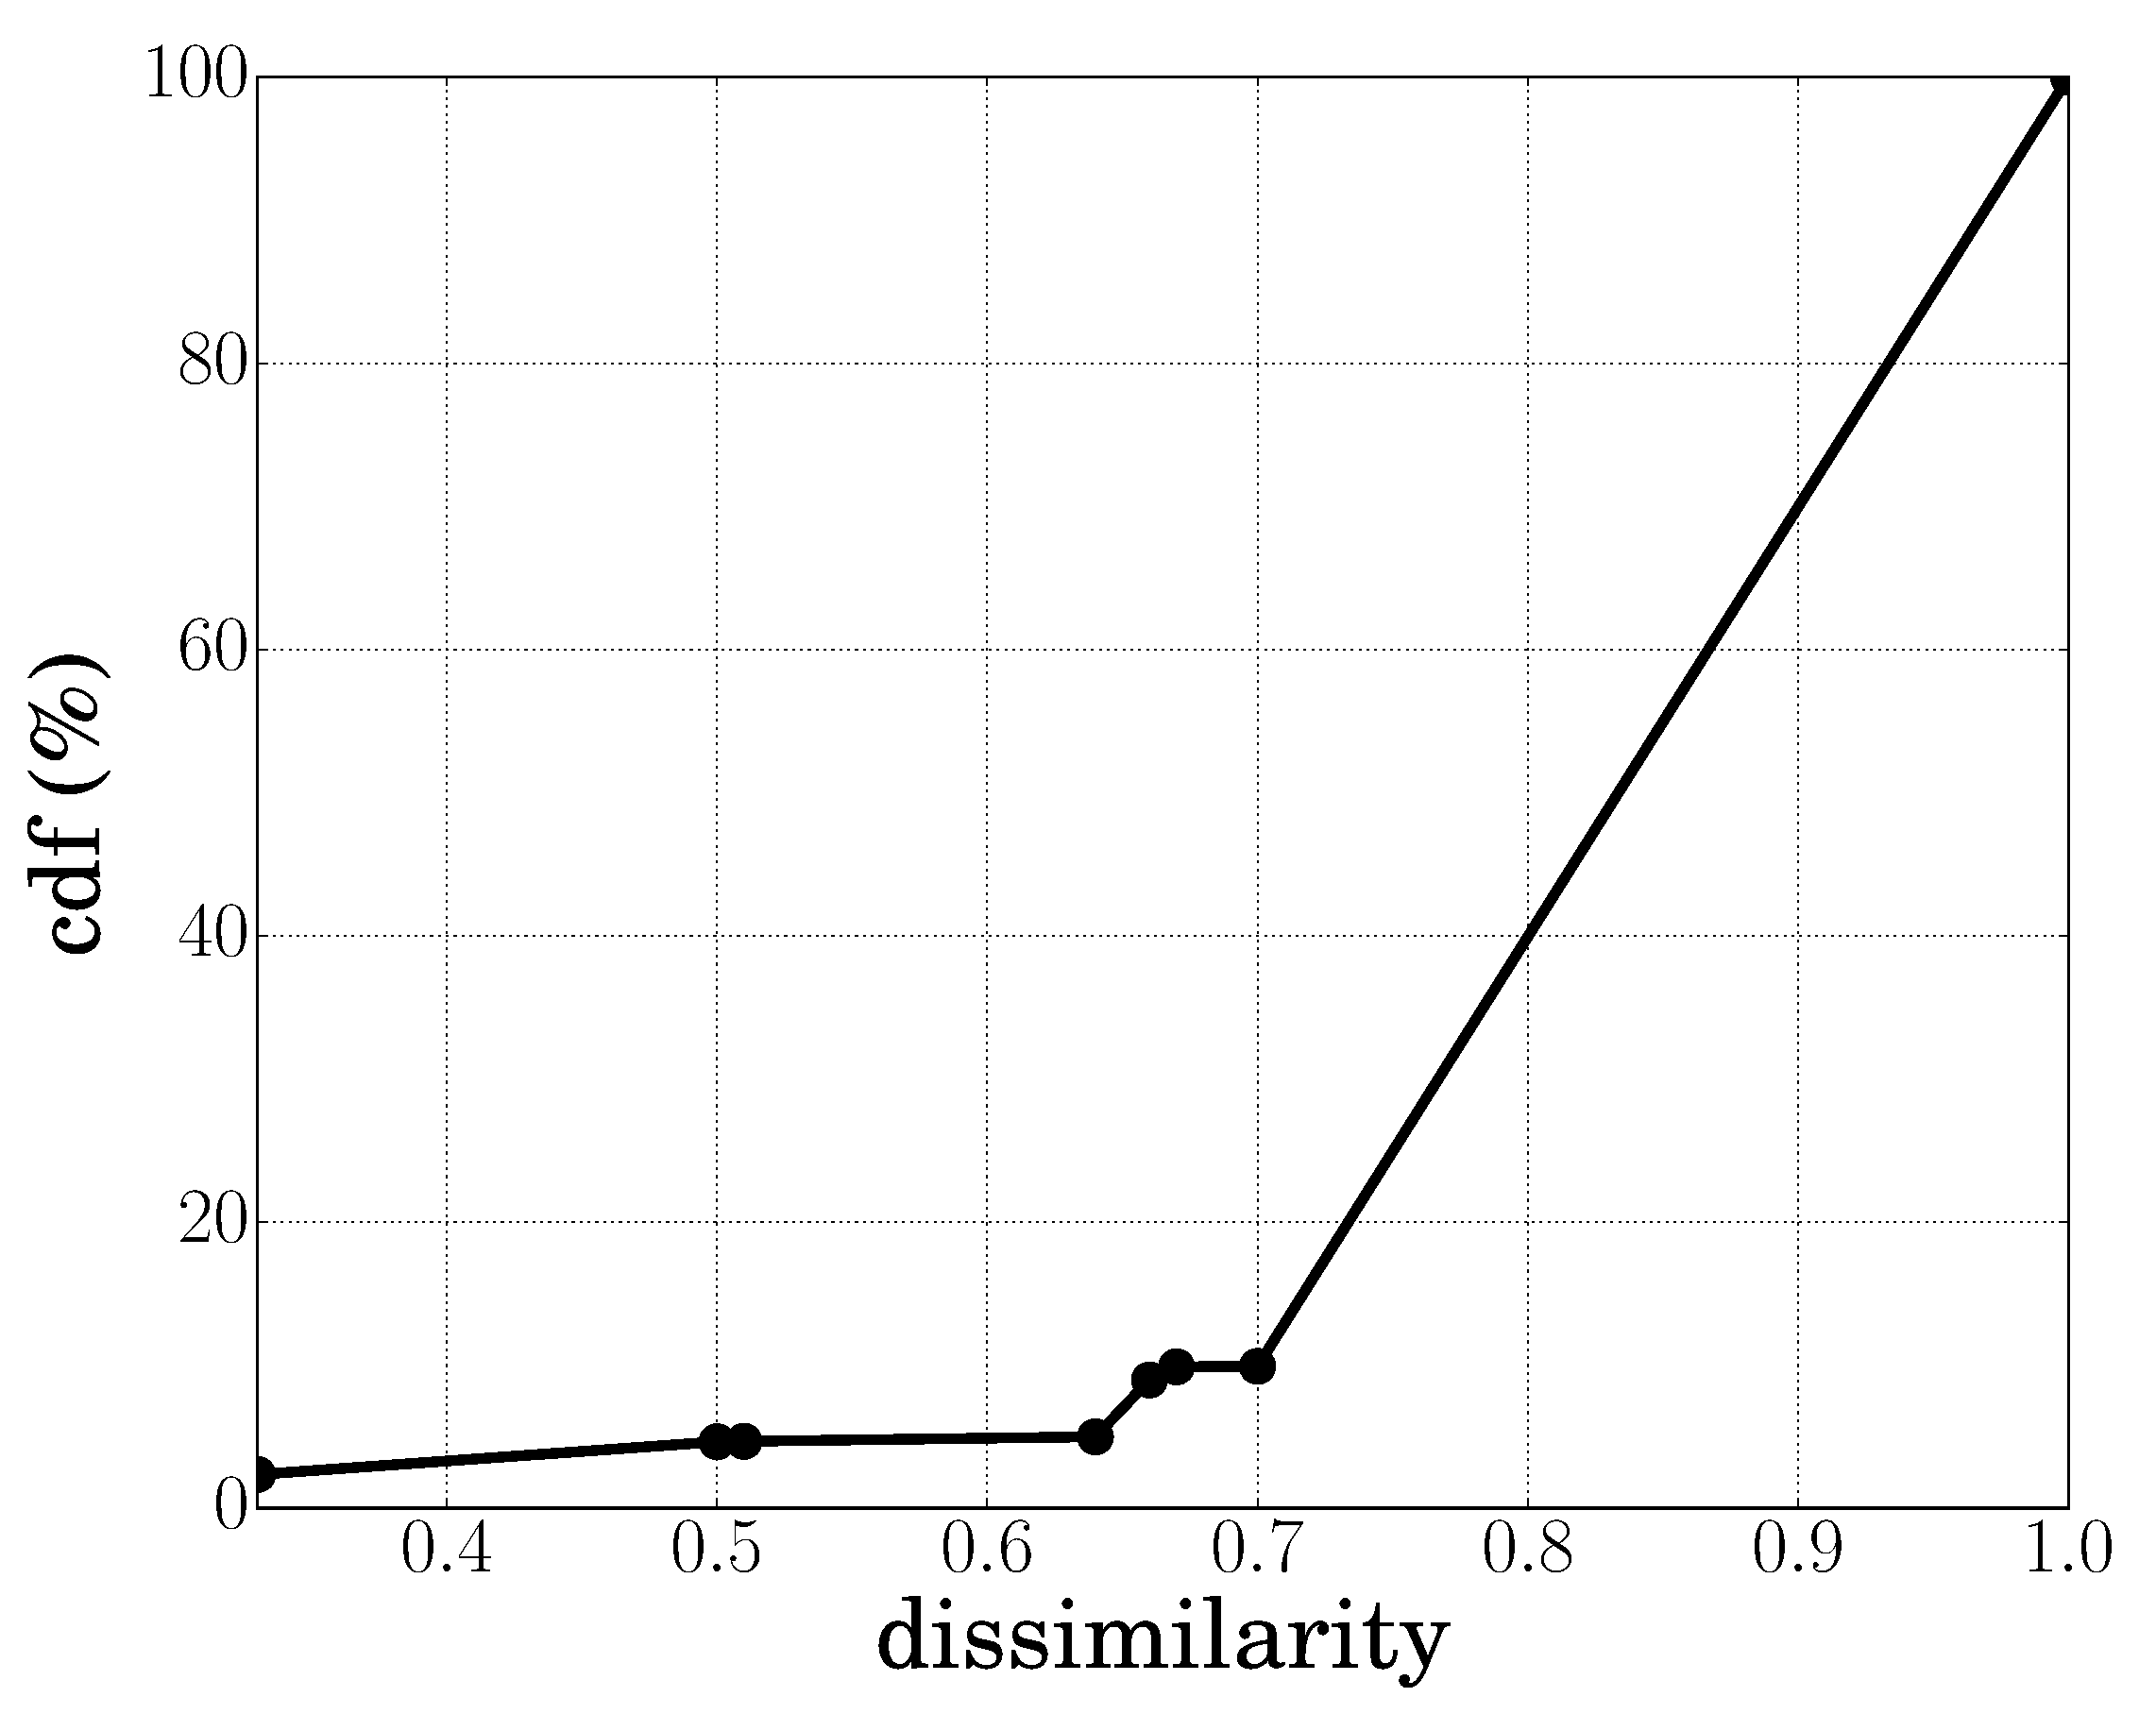
\includegraphics[width=0.7\textwidth]{Pics/cdf_dissmilarity.eps}
	\caption{CDF of the dissimilarity among different types of instabilities.}
	\label{fig:cdf_dissmilarity}
\end{figure}
%-< END FIGURE >-----------------------------------------------------------------

To characterize the mapping changes happening during instabilities, we derived the following \emph{dissimilarity} metric $d(m_i,m_j) = 1 - \frac{ \left|m_i \cap m_j\right|}{\left|m_i \cup m_j\right|}$, based on the Jaccard similarity coefficient, where $m_x$ is the RLOC set of mapping $x$. A dissimilarity of 1 indicates that no RLOCs are shared between the two compared mappings, while a dissimilarity of 0 indicates that the RLOC sets are the same. Fig.~\ref{fig:cdf_dissmilarity} shows the CDF of the mappings' dissimilarity for each unstable <$EID, MR, VP$> tuple. In our experiment, the dissimilarity results are discrete (as the discrete points shown in the Fig.~\ref{fig:cdf_dissmilarity}) in a range from 0.33 to 1.0. As one can expect, the most likely dissimilarity is 1 in 90.09\% of the total number of instabilities. These observations mostly come from New deployment case where before turning on the xTR, no RLOC is provided with the Negative Map-Reply (RLOC set is empty), hence, switch to a LISP Map-Reply implies a full change in the RLOC set. As 90.09\% is larger than the 72.36\% of New deployments share, it indicates as well that complete change of the RLOC set have also been observed during Reconfiguration and Statistical outliers. For the rest, no particular trend can be observed showing that changes of RLOC set can actually take any form.


%-< SECTION >--------------------------------------------------------------------
\section{Mapping System Consistency Evaluation}
\label{sec:mds_consistency}
% In this section, we discuss the consistency of the mapping system respectively by MR and by VP.

In this section, we discuss the consistency of the mapping system respectively by MR and by VP. More precisely, we consider that a tuple of <$EID, *, VP$> exhibits consistency, if all the Map-Replies from different MRs, for a certain EID, observed at a given VP are identical at the same time (same experiment round). This kind of consistency is denoted as \emph{consistency by MR}. Similarly, if all the Map-Replies sent by a specific MR, for a certain EID, and observed at different VPs are identical at every experiment round, then we consider that a tuple of <$EID, MR, * $> is consistent, and denote it as \emph{consistency by VP}. Otherwise, for cases not falling in the above two, we simply say that there exists \emph{inconsistency}. 

Overall, throughout the whole dataset, we found that 86.3\% of observations of all <$EID, *, VP$> tuples are consistent, which indicates that non-identical Map-Replies from different MRs are uncommon. Similarly, consistency by VP is observed in 90.48\% of observations of all <$EID, MR, * $> tuples, showing that the Map-Replies received at different VPs are usually identical. In the following, Sec.~\ref{subsec:mds_consistency_MR} will go deeper in the analysis of consistency by MR, proposing as well several types of inconsistency; then Sec.~\ref{subsec:mds_consistency_VP} will provide thorough analysis of consistency by VP.


%-< SUB SECTION >--------------------------------------------------------------------
\subsection{Consistency Evaluation by MR}
\label{subsec:mds_consistency_MR}
% \begin{itemize}[noitemsep,topsep=0pt]
%     \item The overall percentage of consistency by MR is 86.3\%.
%     \item CDF of the inconsistency frequency by MR.
%     \item For the inconsistency by MR, we classify into 2 cases:
%     \begin{itemize}[noitemsep,topsep=0pt]
%         \item Map-Reply Type: is around 98.34\%.
%         \item RLOC set: 1.66\%.
%     \end{itemize}
% \end{itemize}

The overall percentage of consistency by MR is 86.3\% (see the dashed line on Fig.~\ref{fig:Percentage_consistency_5VP_MR}), meaning that across the whole experiment traces the inconsistency among the Map-Replies sent by different MRs is not common. Yet, we can also observe from Fig.~\ref{fig:Percentage_consistency_5VP_MR} that different VPs show some deviations from the overall consistency by MR, reflecting the fact that while certain VPs receive the same Map-Reply from different MRs, some other VPs receive inconsistent responses. Such deviation is very small (no more than 2.77\%) among different vantage points, indicating that it remains a relatively rare event. These results show that the mapping system is consistent among different MRs in general, but the inconsistency exists at the same time with a percentage around 13.7\%.  In the following of this section, we go deeper this issue, exploring the reasons why the few observations exhibit
inconsistency by MR.

%-< FIGURE >--------------------------------------------------------------------
\begin{figure}[!t]
	\centering
	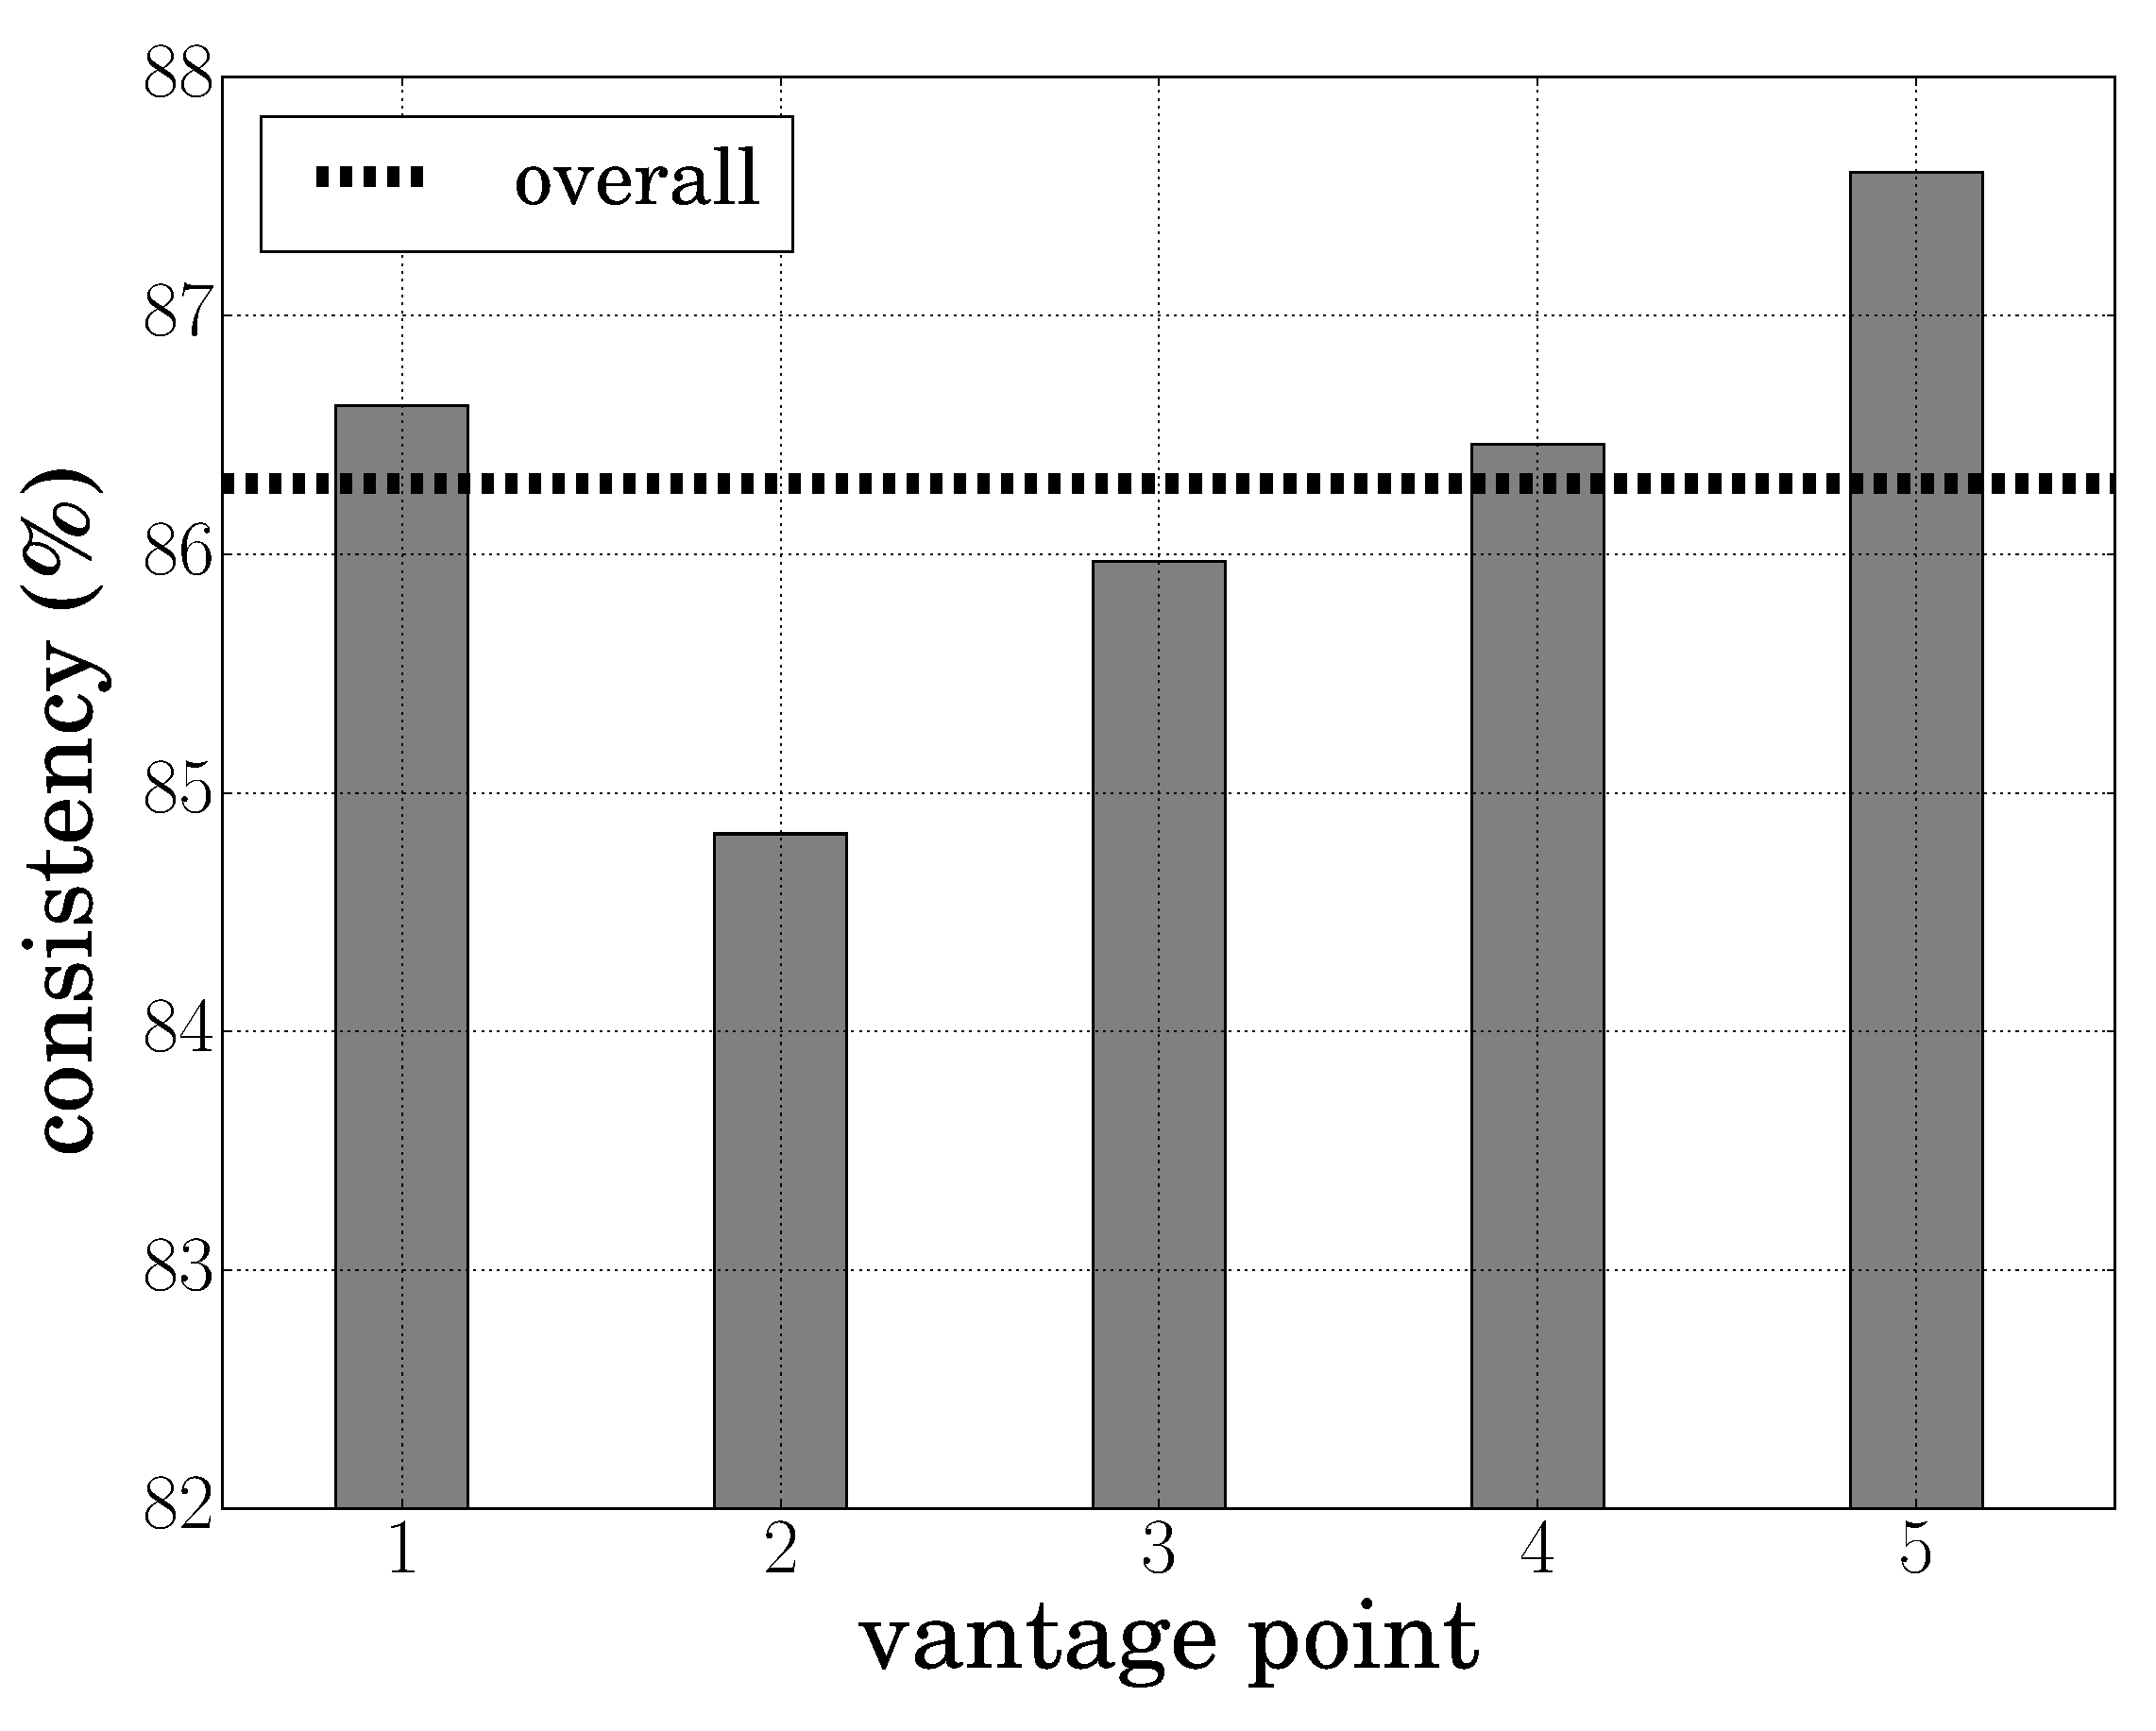
\includegraphics[width=0.7\textwidth]{Pics/Percentage_consistency_5VP_MR.eps}
	\caption{Overall consistency by MR at 5 different Vantage Points.}
	\label{fig:Percentage_consistency_5VP_MR}
\end{figure}
%-< END FIGURE >--------------------------------------------------------------------

We compute the CDF of the inconsistency frequency by MR: $f_{<EID, *, VP>}$, i.e.,  the probability of inconsistency frequency over all <$EID, *, VP$> tuples, by using the following definition: 
\begin{equation}
f_{<EID, *, VP>}= \frac{\text{\# Inconsistencies by MR}}{\text{\# Experiments}}\times100\%.
\end{equation}
For a <$EID, *, VP$> tuple, an inconsistency frequency of 0\% means that all Map-Replies from all of the different MRs for one EID are the same at each experiment round throughout the whole measurement campaign.  For a <$EID, *, VP$> tuple, an inconsistency frequency of 100\% means that at each experiment round during the whole measurement campaign, there is at least one MR replying a Map-Reply different from the replied by other MRs. The resulting CDF of inconsistency frequency is shown on Fig.~\ref{fig:cdf_incons_occur_MR}. The value 0\% of inconsistency frequency has a probability of 82.38\%, indicating that through all the dataset, there are 82.38\% of <$EID, *, VP$> tuples that are always consistent by MR at whichever VP. Yet, it is worth noticing that this value is lower than the overall consistency of 86.3\% shown in Fig.~\ref{fig:Percentage_consistency_5VP_MR}. The reason of such difference lays in the fact that, when we analyze the 0\% inconsistency frequency, we just take into account those common EIDs exhibiting a consistency by MR in all VPs. Hence 82.38\% represents the subset of the EIDs considered in the former percentage and is the lower bound, guaranteeing that 82.38\% of <$EID, *, VP$> tuples always have consistent responses, regardless of the VP. In addition, the inconsistency frequency concentrates at a very low range, since a sharp increase occurs between 0\% and 2\% with a growth of 16.15\%. % (98.53\% - 82.38\%). 
It indicates that the <$EID, *, VP$> tuples classed as inconsistent do actually receive inconsistent responses rarely, hence, demonstrating that the mapping system is generally consistent. Yet, in very few cases (only 0.5\%), the inconsistency between different MRs occurs all the time.

%-< FIGURE >--------------------------------------------------------------------
\begin{figure}[!t] 
	\centering
	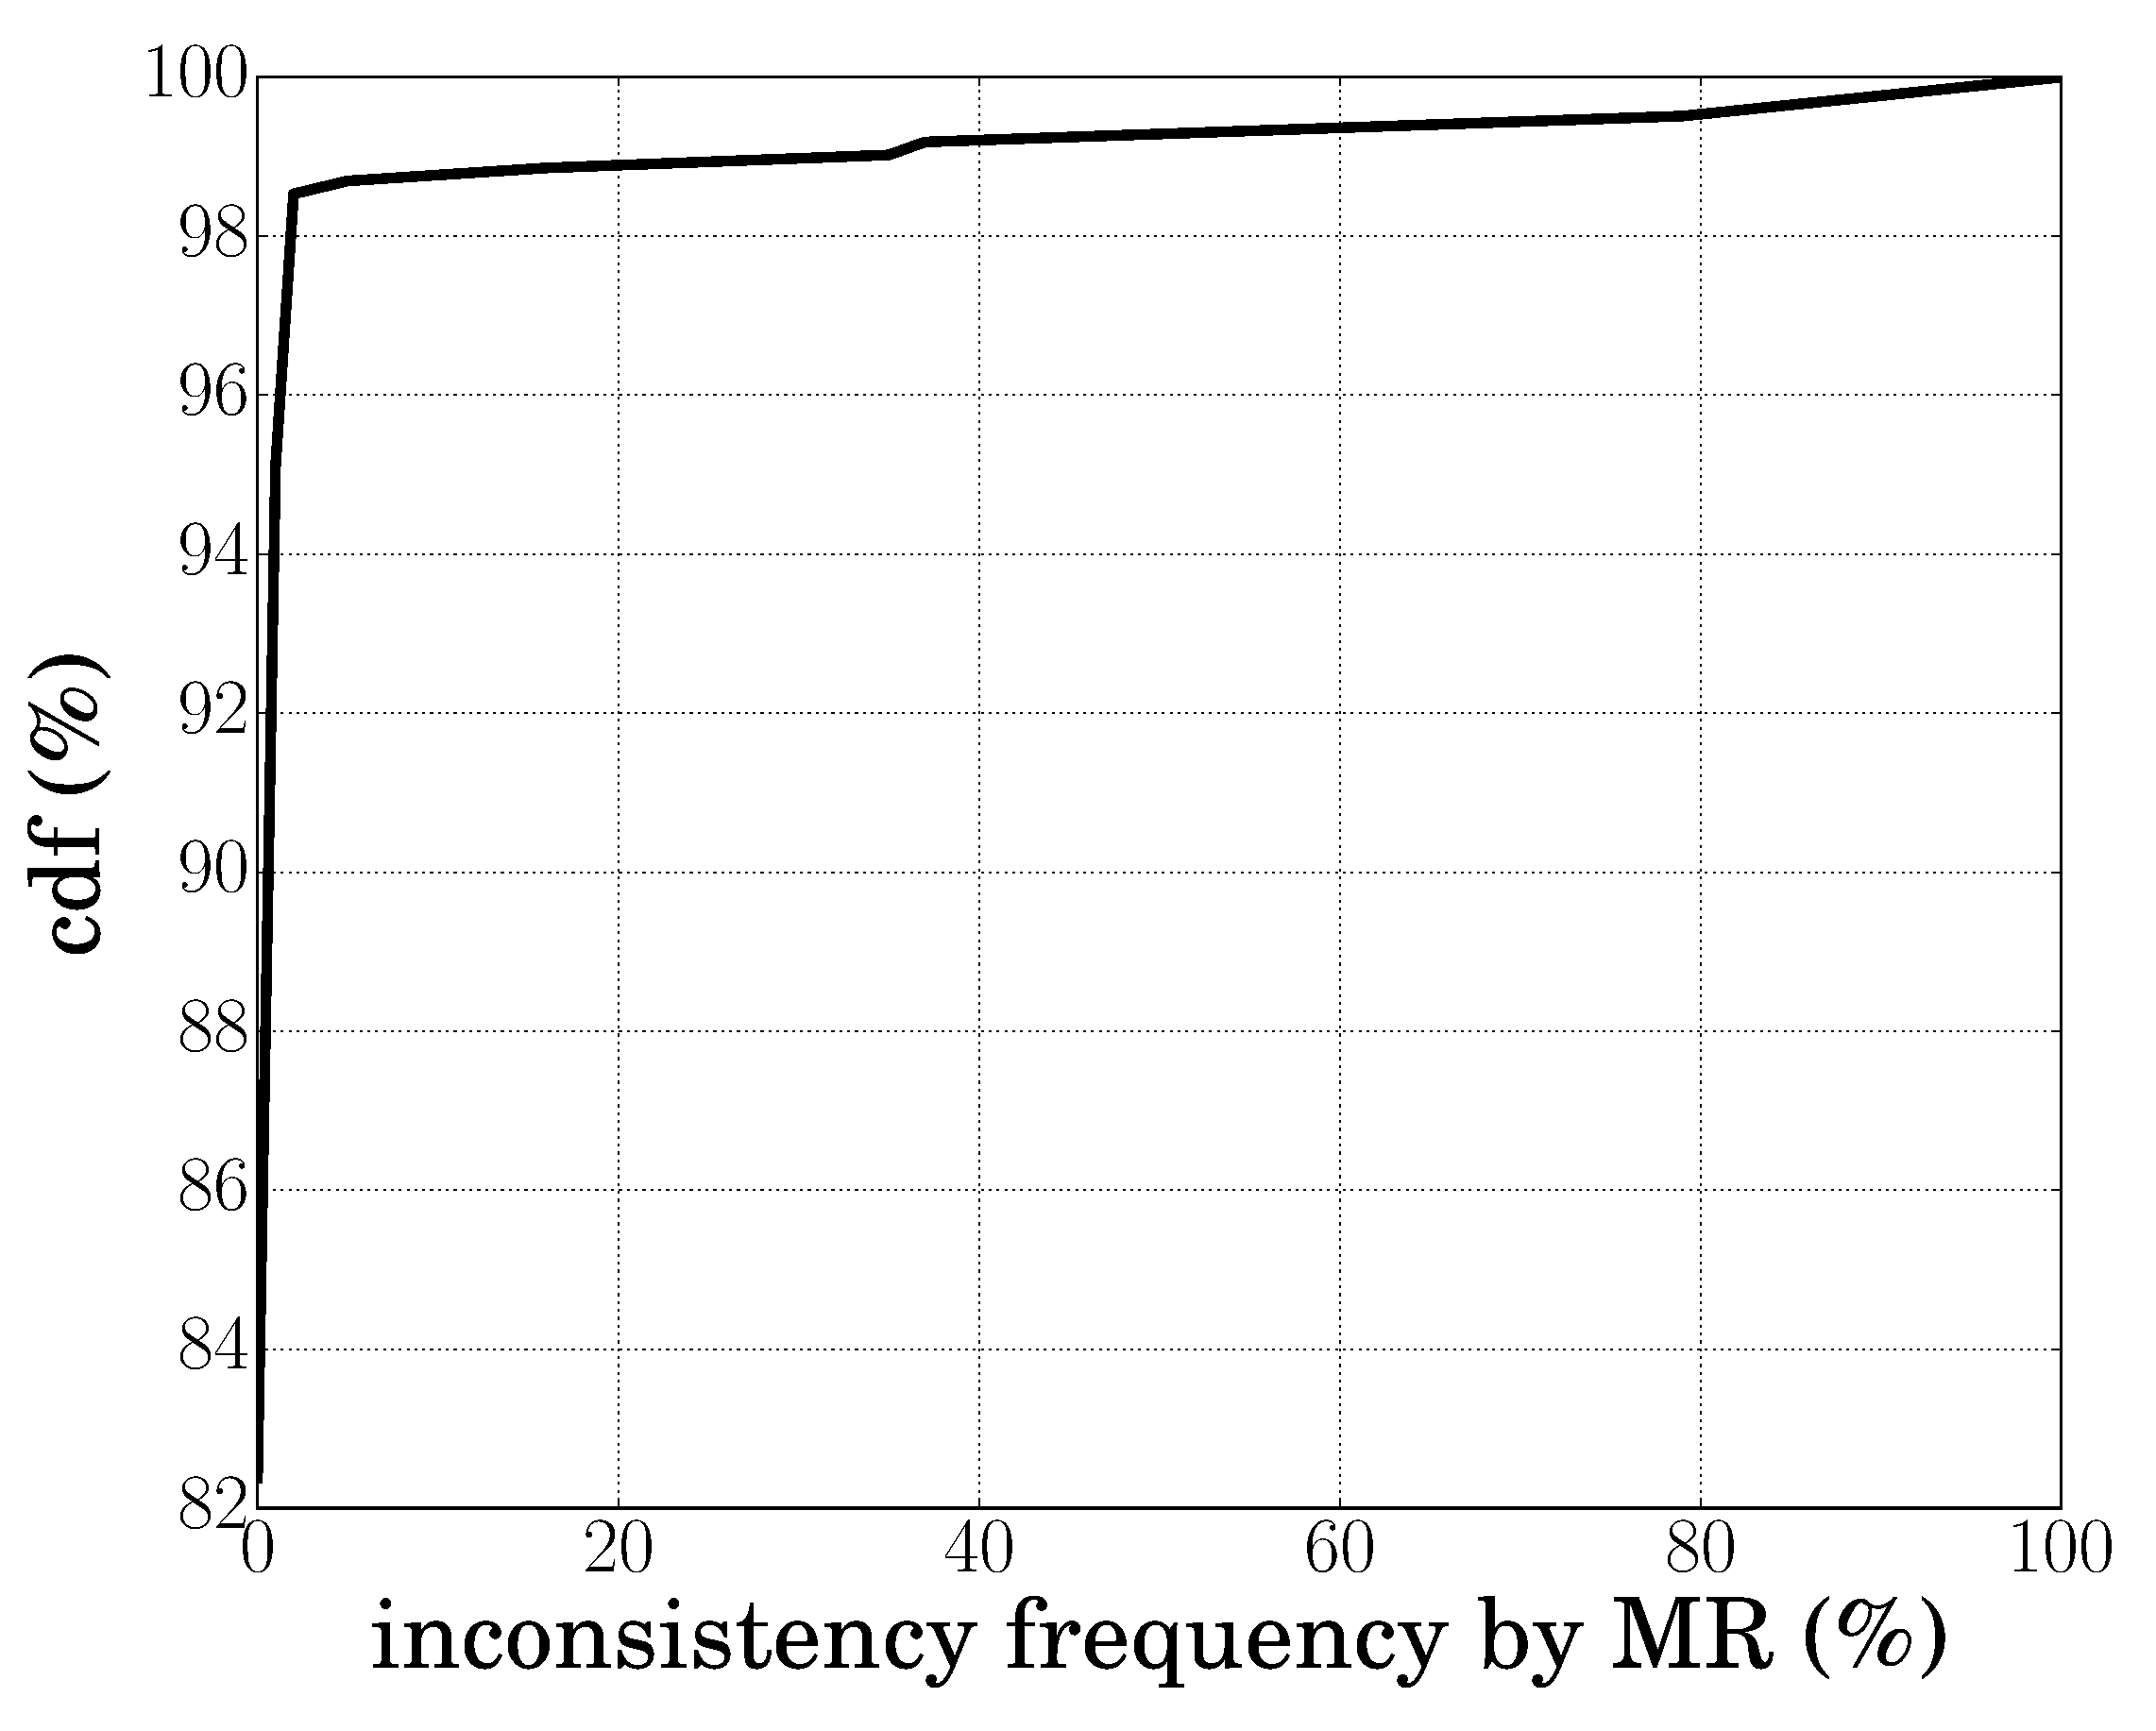
\includegraphics[width=0.7\textwidth]{Pics/cdf_incons_occur_MR.eps}
	\caption{Cumulative Distribution Function of inconsistency frequency by MR. X-axis is inconsistency frequency by VP, indicating the ratio of inconsistency occurrence for each <$EID, *, VP$> tuple over total experiment number.}
	\label{fig:cdf_incons_occur_MR}
\end{figure}
%-< END FIGURE >--------------------------------------------------------------------

So far, the analysis indicates that the mapping system is consistent by MR in general, but the inconsistency indeed exists. To have a closer look to the inconsistency, we further cluster it into two cases:
\begin{itemize}[noitemsep,topsep=0pt]

\item \textbf{Map-Reply Type}:, The type of Map-Reply provided by the 13 MRs for a specific <$EID, *, VP$> tuple is different, meaning that some MRs provide LISP Map-Reply while others return a Negative Map-Reply. The difference of received Map-Reply type leads the xTRs to use a different way to send the packets, i.e., xTRs receiving a LISP Map-Reply sends LISP-encapsulated packets by using the obtained RLOCs, while xTRs receiving a Negative Map-Reply will forward the conventional packets (i.e., without LISP-encapsulation).
\item \textbf{RLOC set}: All the Map-Replies returned by the 13 MRs for a <$EID, *, VP$> tuple belong to LISP Map-Reply type, but the associated attributes (cf.  Tab.~\ref{tab:List_of_possible_changes} from Sec.~\ref{sec:mds_methodology}) are different.  For instance, some Map-Replies may contain RLOC$_1$, while some others convey RLOC$_2$ (i.e., the RLOC address is not identical); or some Map-Replies have only one RLOC, whereas others have multiple RLOCs (i.e., the RLOC number is different), and so on. The difference in such Map-Replies could lead the requesting xTRs to select different destination RLOCs. 
\end{itemize}

The large majority of inconsistencies, around 98.34\%, are Map-Reply Type, probably because there is an update of mapping information in the mapping system for the New Deployment case. Not all of the 13 MRs simultaneously update the mapping information, meaning that a convergence time is needed so that the global mapping information maintained in all parts of the mapping system is synchronized. If VPs query the mapping system during this convergence period, some MRs will still provide Negative Map-Replies, while other (already updated) MRs will forward the Map-Requests towards the corresponding ETRs, which in turn will send the updated LISP Map-Replies, and vice versa. This situation contributes to the inconsistency frequency around 1\%, which means that there is only once or twice inconsistency between Map-Replies from different MRs for one specific EID, since changing the status of xTR is not frequent.

Just few inconsistencies, only 1.66\%, are caused by the RLOC set. This scenario usually occurs for those EIDs whose RLOCs change frequently over time (the case of Statistical outliers instability). So, because of the convergence time of the mapping system, it is very difficult to guarantee that every MR can provide the same LISP Map-Reply at every experiment round. This reason for changes in the RLOC set is most probably due to traffic engineering policies. Similarly as the previous case, when different MRs provide a different RLOC set for a specific EID, the requesting xTRs may end up using different RLOCs to reach the same destination EID.
 

%-< SUB SECTION >--------------------------------------------------------------------
\subsection{Consistency Evaluation by VP}
\label{subsec:mds_consistency_VP}
% \begin{itemize}[noitemsep,topsep=0pt]
%     \item The overall percentage of consistency by VP is 90.48\%.
%     \item CDF of the inconsistency frequency by VP.
%     \item For the inconsistency by MR, we classify into 2 cases:
%     \begin{itemize}[noitemsep,topsep=0pt]
%         \item Map-Reply Type: is around 89.06\%.
%         \item RLOC set: 10.94\%.
%     \end{itemize}
% \end{itemize}

%-< FIGURE >--------------------------------------------------------------------
\begin{figure}[!t]
	\centering
	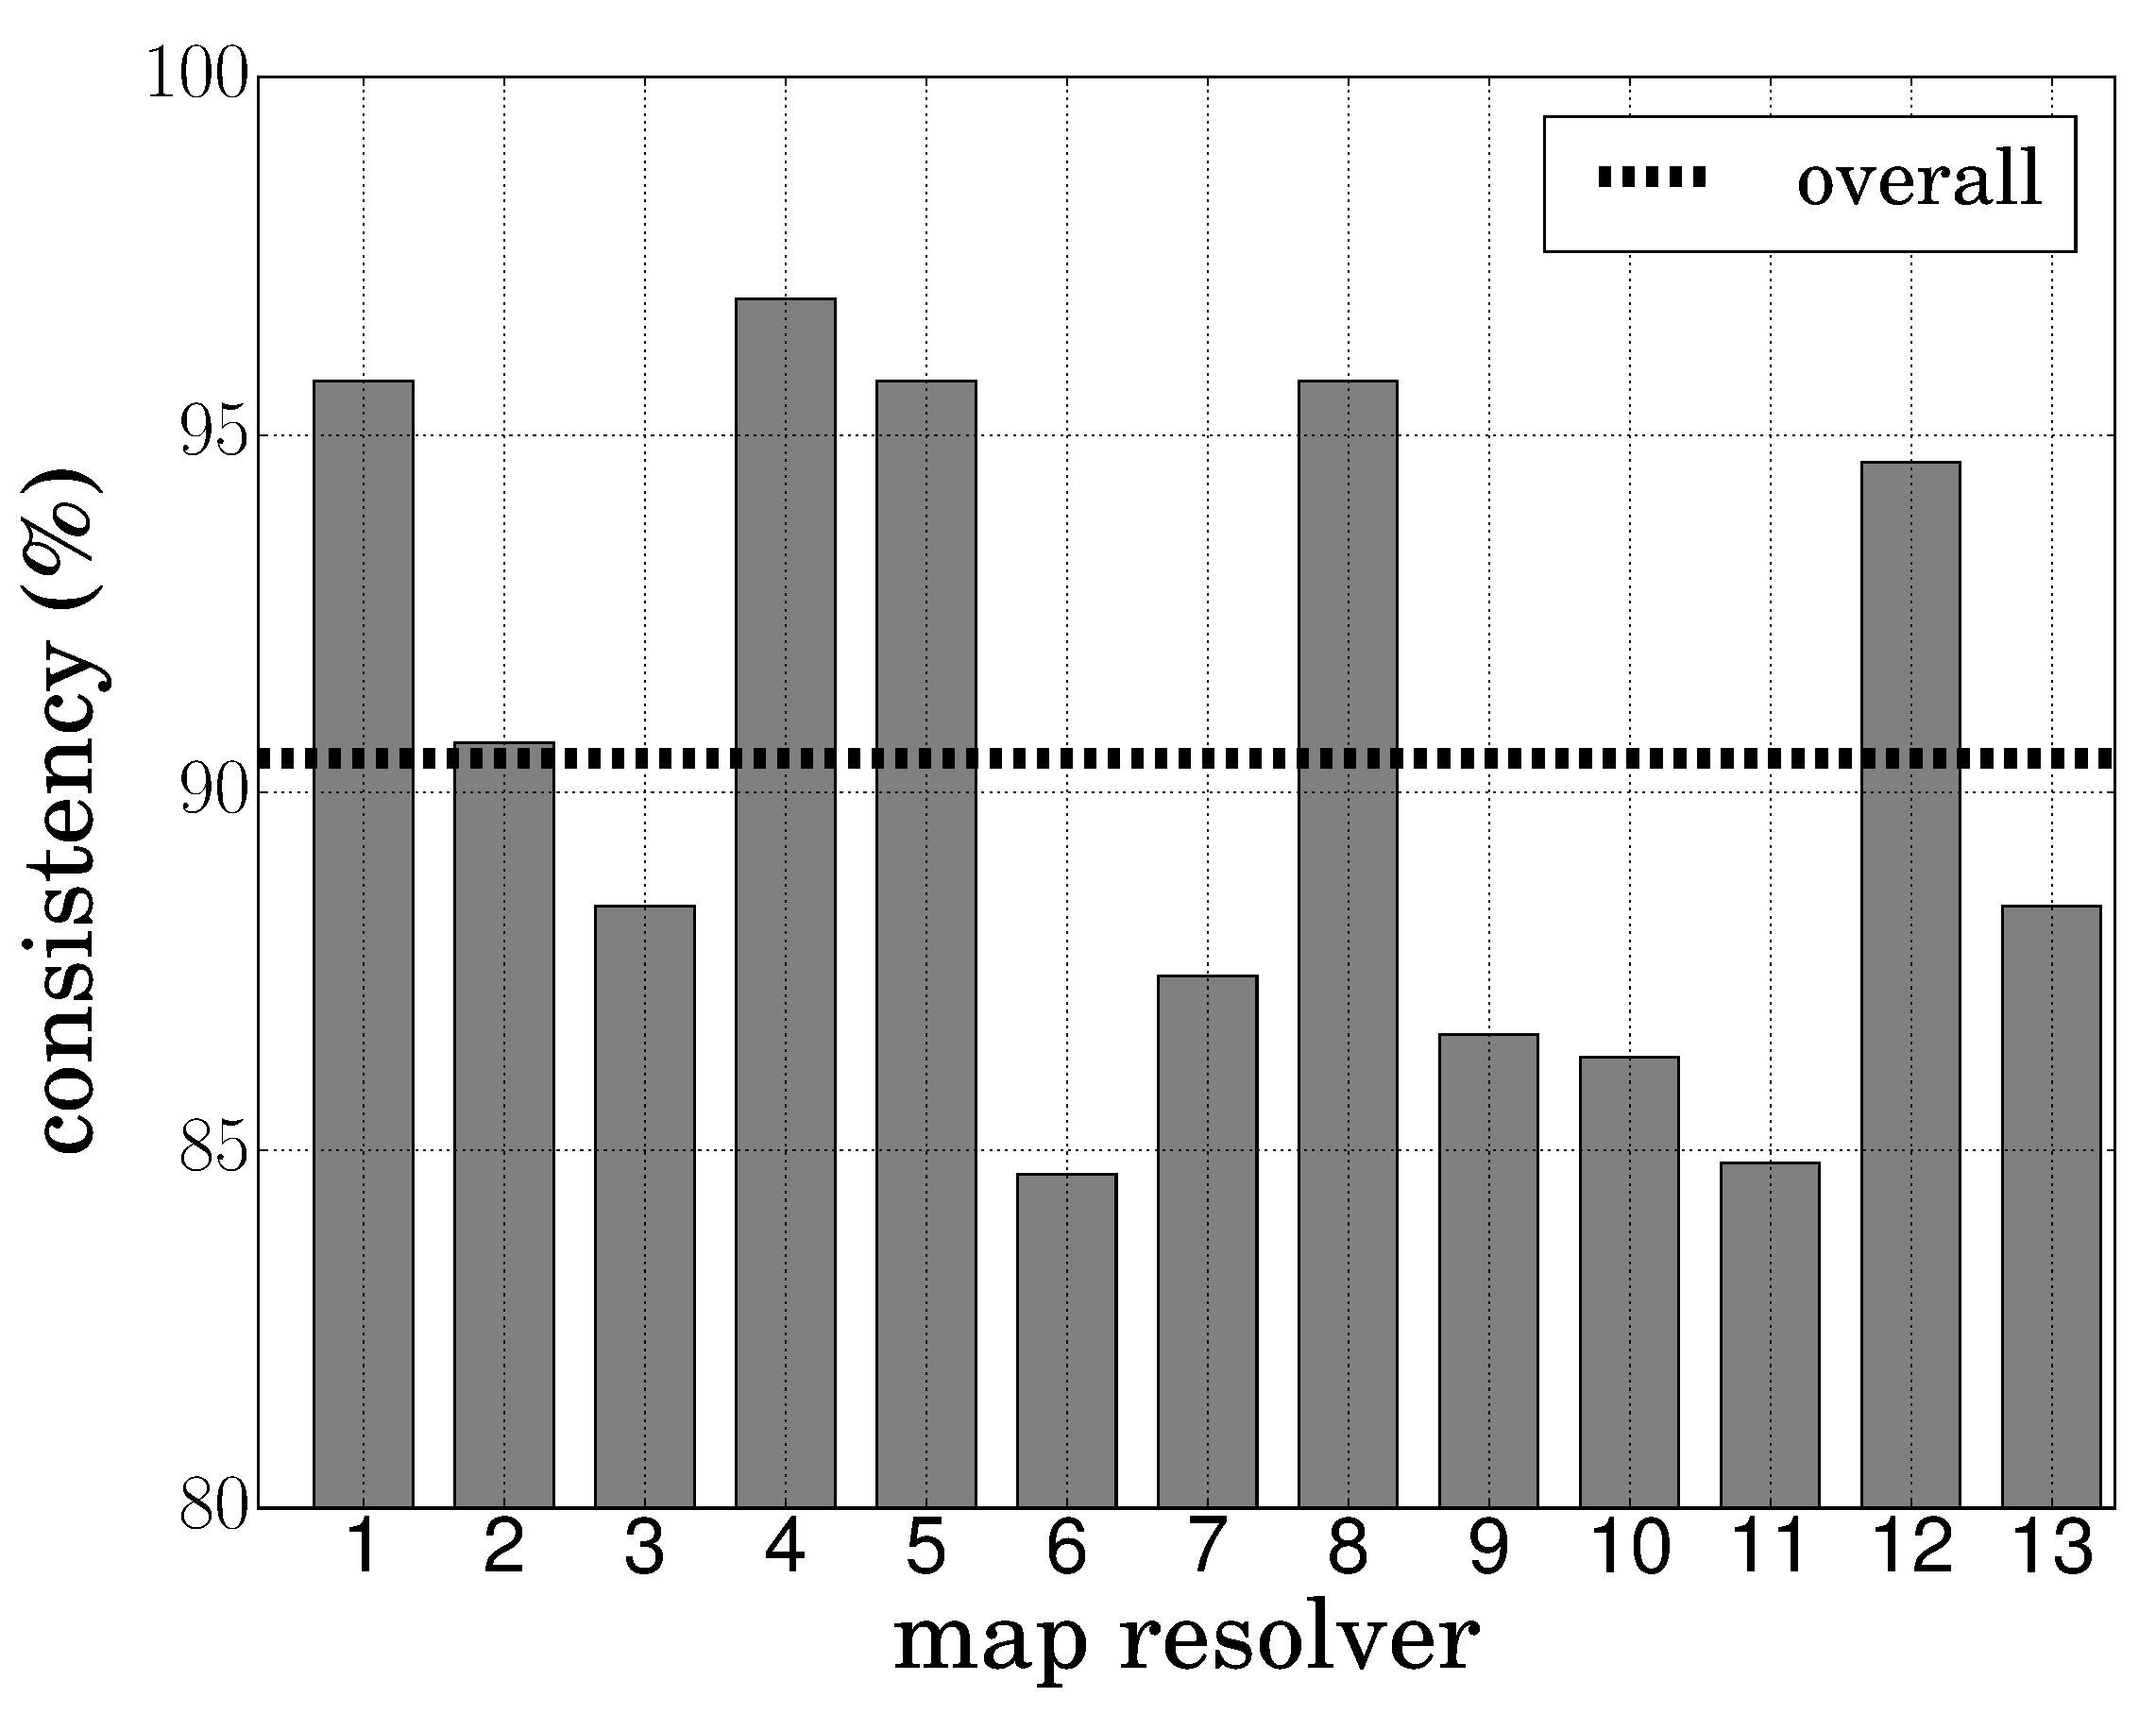
\includegraphics[width=0.7\textwidth]{Pics/Percentage_consistency_13MR_VP.eps}
	\caption{Overall consistency by VP from the different Map-Resolvers.}
	\label{fig:Percentage_consistency_13MR_VP}
\end{figure}
%-< END FIGURE >--------------------------------------------------------------------

The overall percentage of consistency by VP for the whole experiment dataset is 90.48\%, presented by the dotted line in Fig.\ref{fig:Percentage_consistency_13MR_VP}, which indicates that the Map-Replies received at different VPs from the same MR are highly consistent. Yet, we can also observe that different MRs show some deviations from the overall consistency by VP, reflecting the fact that certain MRs send the same Map-Reply to all VPs, but some do not. The deviation among different MRs is however limited (less than 12.23\%). Therefore, we can certainly state that the mapping system shows generally a high degree of consistency by VP but presents a non-negligible amount of inconsistencies (9.52\%). In the rest of this section, following the same approach as for the consistency by MR, we go deeper this issue, exploring the reasons why some observations exhibit inconsistency by VP.

%-< FIGURE >--------------------------------------------------------------------
\begin{figure}[!t]
	\centering
	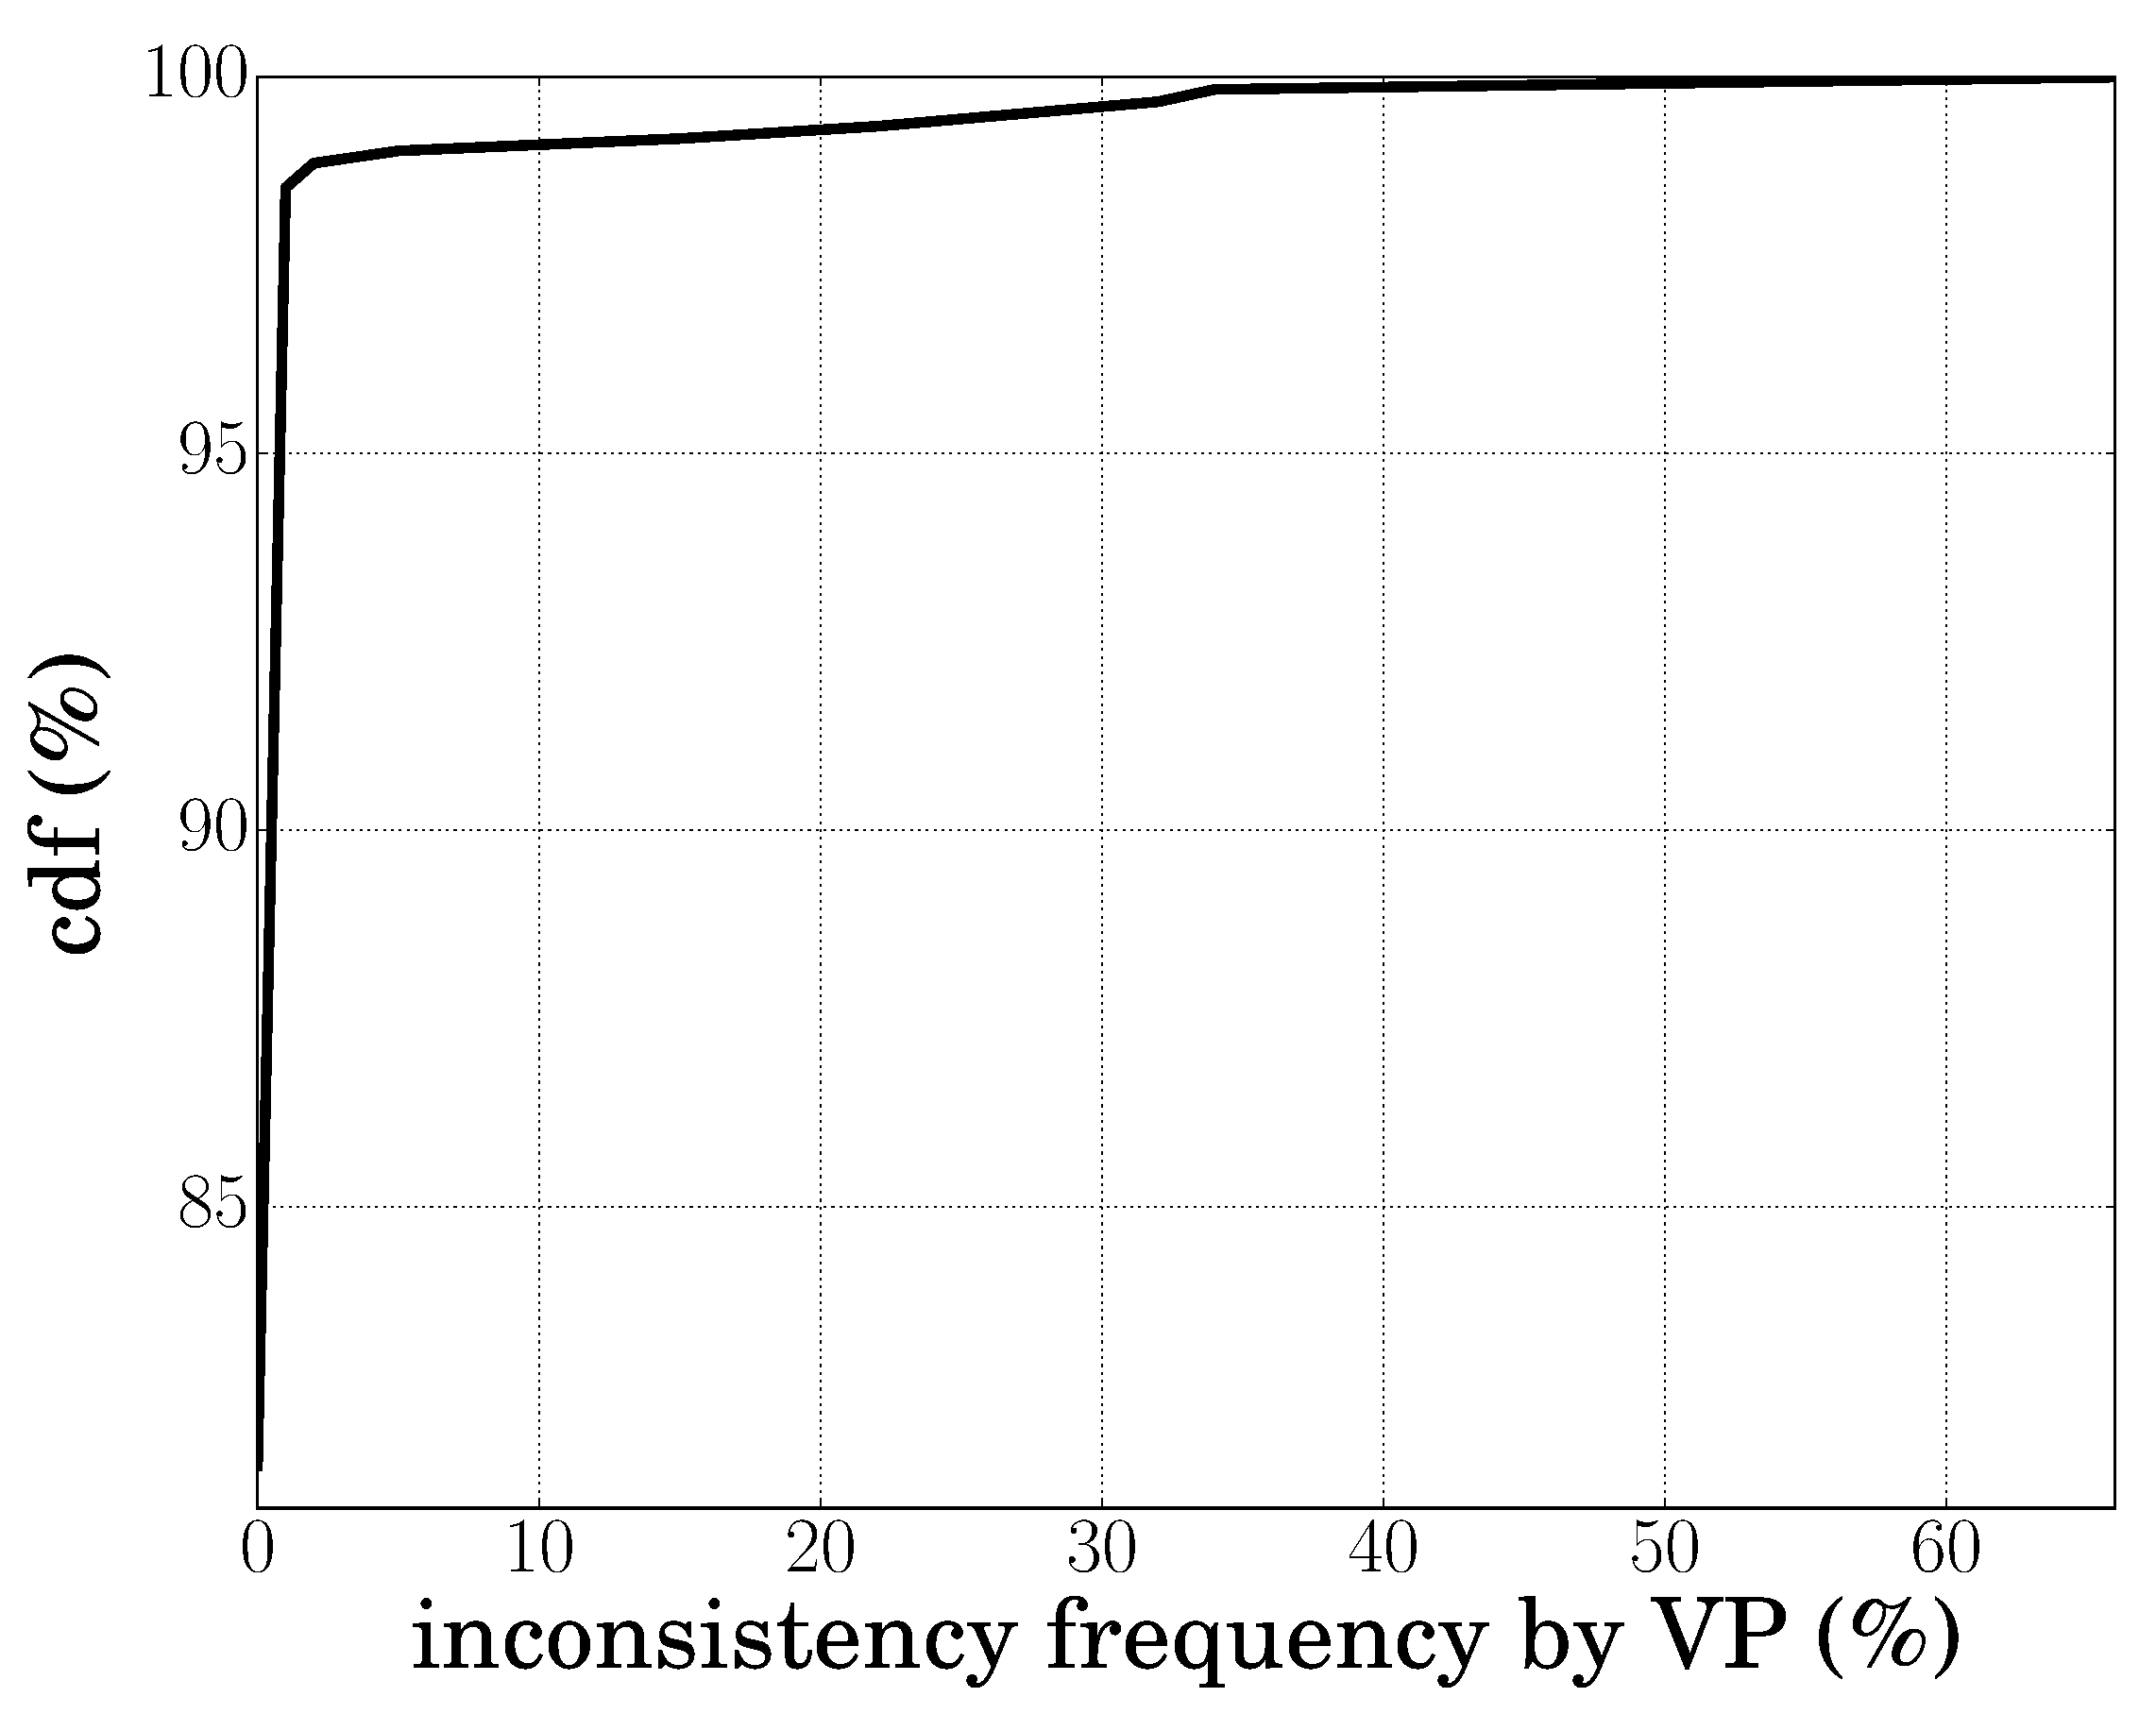
\includegraphics[width=0.7\textwidth]{Pics/cdf_incons_occur_VP.eps}
	\caption{Cumulative Distribution Function of inconsistency frequency by VP. X-axis is inconsistency frequency by VP, indicating the ratio of inconsistency occurrence for each <$EID, MR, *$> tuple over total experiment number.}
	\label{fig:cdf_incons_occur_VP}
\end{figure}
%-< END FIGURE >--------------------------------------------------------------------

Fig.\ref{fig:cdf_incons_occur_VP} shows the CDF of the inconsistency frequency by VP: $f_{<EID, MR, *>}$, i.e., the probability of inconsistency frequency for all <$EID,MR,*$> tuples, by using the following definition: 
\begin{equation}
f_{<EID, *, VP>} = \frac{\text{\# Inconsistencies by VP}}{\text{\# Experiments}}\times100\%.
\end{equation}
Like for the explanation for Fig.~\ref{fig:cdf_incons_occur_MR}, here an inconsistency frequency by VP of 0\% means that all Map-Replies received by all of the VPs from a same MR are totally consistent at every experiment round during the whole experiment campaign, while an inconsistency frequency of 100\% means that at least one of VPs received an inconsistent Map-Reply compared to the other VPs at every experiment round. The probability of consistency by VP (when X-axis is 0\% in Fig.~\ref{fig:cdf_incons_occur_VP}) is similar to that by MR, with a value of 81.57\%. It can be noticed that this percentage is slightly lower than the overall percentage of consistency by VP in Fig.~\ref{fig:Percentage_consistency_13MR_VP}. The reason is that here the inconsistent occurrence with 0\% only includes those EIDs for which all VPs always show consistency, no matter which MR is actually queried. A sharp increase with a growth of 16.97\% % (98.53\% - 81.56\%) 
is found when X-axis is 1\%, which means that although VPs sometimes receive inconsistent Map-Replies at several experiment rounds, the occurrence remains pretty low, hence showing that even by VP  the mapping system exhibits a very high degree of consistency. Differently from the largest inconsistency frequency by MR, which goes up to reaches 100\%, the largest inconsistency frequency by VP is only 66\%. This phenomenon indicates a fact that the Map-Replies received by different VPs are not inconsistent all the time, at least there are one third of observations show that their Map-Replies are totally same. Thus the consistency by VP is higher than consistency by MR.

To further explore the inconsistency by VP, we then use same metrics as in Sec.~\ref{subsec:mds_consistency_MR}, with the exception that the queried target changes from <$EID, *, VP$> to <$EID, MR, *$> tuples.

The most inconsistent case, 89.06\%, is due to a mix of Negative Map-Reply and LISP Map-Reply, i.e., demand for a same <$EID, MR, *$> tuple, at some VPs receive Negative Map-Reply but at others receive LISP Map-Reply. This is caused by the New Deployment case, but differently from the cause for inconsistency by MR, the reason for inconsistency by VP is probably because of Map-Requests sent by different VPs can not be processed exactly at the same time, due to queuing in the MR. Thus, if the queries are sent during the period of mapping information update, some VPs, whose Map-Requests are processed first will have different Map-Reply Type from the latter ones. Inconsistencies caused by different RLOC sets, i.e., different VPs receive LISP Map-Replies with different RLOCs set from the same MR, also exist, contributing for around 10.94\%. It is probably caused by a combination of the Statistical outliers instability case and the queuing mechanism in MR. As the RLOC sets provided by a MR for some certain EIDs frequently change, and the Map-Requests sent by different VPs need to be processed one by one, it is very possible that the first processed Map-Requests are replied by the different RLOC sets compared to the latter ones. The difference between Map-Replies is probably due to traffic engineering policies, but the further experiments are needed to explore the deeper reasons for such inconsistency.



%-< SECTION >--------------------------------------------------------------------
%\section{LISP-related Discussion and Conclusion}
\section{Summary}
\label{sec:mds_conclusion}
% \begin{itemize}[noitemsep,topsep=0pt]
%     \item Measurements show that the LISP mapping system is stable and consistent over time. 
%     \item Nevertheless, instability and inconsistency are observed but are rare events.
%     \item We developed a new taxonomy to deeper study instability and inconsistency.
%     \item We also provide possible reasons causing the instability and inconsistency, but need future proves.
% \end{itemize}

During the evaluation of LISP mapping system performance, besides the observations about the stability and consistency that we describe in details in the previous sections, we also investigate some interesting LISP-related results. We provide them here so that they can be used to improve LISP performance. We identified that 8.97\% of the LISP-sites leverage on multiple RLOCs in order to be multihomed to the Internet, with an average of 3 distinct locators. Interestingly, when we compare the locators with their Autonomous System Number we found that around 50\% of the locators in multihoming situations belong to different ASes, which indicates that LISP is used to transparently interconnect LISP-sites by the intermediate of multiple ISPs.\footnote{We used the Team Cymru BGP database to associate IP addresses to ASNs (see \url{http://www.team-cymru.org/IP-ASN-mapping.html}).} As the control-plane (i.e., MS/MR and mapping system) and the data-plane (i.e., ETR/ITR) are decoupled in LISP, Map-Replies can originate from the LISP-sites directly or from shared utilities constituting the mapping system (i.e., MS/MR). This particularity of LISP is already used in the current deployment, where only 88.8\% of the non-negative Map-Replies are originated directly from their LISP-sites, with the remaining 11.2\% being originated by delegated MSes replying on behalf of the LISP-sites. This allows reducing the control traffic seen by LISP-sites and help them to scale better.

In addition to mappings, LISP also relies on encapsulation, meaning that with LISP traffic can be transported over IPv4 or IPv6 without requiring end-hosts to be dual-stack. Interestingly, we identified that no less than 8.84\% of the locators are IPv6. However, we have not observed cases where a LISP site was reachable strictly using IPv6 while 82.79\% of sites are reachable only through IPv4. This discrepancy tends to confirm that network operators still lack of confidence being reachable only through IPv6. As a result, the 17.21\% of LISP-sites explicitly using IPv6, always include at least one IPv4 address in order to be reachable.

As a solution to cope with the increase of BGP routing table, traffic engineering, and scalability issues, LISP has been widely deployed on the LISP Beta Network experimental testbed for ten years. To ensure accurate and efficient communications, LISP mapping system should be stable and consistent. However, there is no study evaluating the stability and consistency of LISP mapping system. For such purpose, we continuously measured the LISP Beta Network for seventeen days to assess the mapping system from these two aspects. Measurements show that the LISP mapping system is stable and consistent over time. Nevertheless, instability and inconsistency are observed and for studying them in details we developed a new taxonomy. All in all, instability and inconsistency are rare events. At last, we observe utilization of multi-homing and dual-stack (i.e., IPv4 and IPv6) during the whole experiment and plan to use these results to further improve the LISP performance. % stability & consistency
%*******************************************************************************
%****************************** Fourth Chapter *********************************
%*******************************************************************************

\chapter{LISP-Views: LISP mapping system monitor}
\label{cha:LISPViews}

% **************************** Define Graphics Path **************************
\ifpdf
    \graphicspath{{Chapter5/Pics/Raster/}{Chapter5/Pics/PDF/}{Chapter5/}}
\else
    \graphicspath{{Chapter5/Pics/Vector/}{Chapter5/}}
\fi

%-< ABSTRACT >--------------------------------------------------------------------
Currently only two LISP experimental platforms have already been deployed in the Internet: LISP Beta Network and LISP-Lab platform. % However, only one monitoring tool exists: LISPmon that crawls the mapping system once a day. To accompany the growth of LISP, a dynamic and complete monitoring system is required. Therefore, we propose LISP-Views, a dynamic versatile large scale LISP monitoring architecture. LISP-Views allows to automatically conduct comprehensive and objective measurements. After running LISP-Views in the wild for several months and comparing the monitoring results with LISPmon, we confirm that LISP-Views provides more detailed and accurate information. We observe the different behaviours between every network entity within the mapping system, and also explore the current LISP performance for further improvements.
Currently, a unique LISP monitoring system called LISPmon~\cite{lispmon} supervises the global \acrshort{mds} and publishes the mapping information daily. However, it is known that the mapping information sometimes changes frequently within a day and that the elements constituting the \acrshort{mds} are not always consistent (more details can be found in Chapter~\ref{cha:mds_evaluation} in this dissertation)~\cite{yue2016stability}. We hence propose a dynamic versatile LISP monitoring architecture, namely LISP-Views, to overcome these limitations. LISP-Views automatically explores the whole \acrshort{mds} every 2 hours and stores the detailed mapping information, so to facilitate the experimenters to evaluate the LISP comprehensive performance.

We used a one-month long set of traces produced by LISP-Views to evaluate its performance and accuracy, including comparing it with LISPmon. We show that LISP-Views is more accurate than LISPmon since it monitors all the \acrshort{mds} elements in parallel. In addition, thanks to its detailed reporting, LISP-Views allows to assess high level metrics of LISP deployments such as reliability, latency, or configuration
issues.

In the remainder, Sec.~\ref{sec:lispviews_archi_motivation} introduces LISPmon and why we propose a new LISP monitor. Sec.~\ref{sec:lispviews_archi_description} describes our proposed LISP monitoring architecture in details. Sec.~\ref{sec:lispviews_evaluation} validates LISP-Views by comparing with LISPmon. Sec.~\ref{sec:lispviews_results} provides the snapshot of what kind of further analysis can be done with our proposal. Finally, Sec.~\ref{sec:lispviews_conclusion} concludes the chapter. 
%-< ABSTRACT >--------------------------------------------------------------------


%\section{Introduction}
%\label{sec:lispviews_introduction}
% \begin{itemize}[noitemsep,topsep=0pt]
%     \item LISPmon is the only LISP monitor providing the basic LISP mapping information.
%     \item It cannot satisfy the more complex requirements and is not able to monitor the whole current LISP mapping system in real time.
%     \item LISP-Views is proposed.
%     \item LISP-Views provides more mapping information than LISPmon.
%     \item LISP-Views offers more specific information that LISPmon cannot provide.
% \end{itemize}
% To promote the development of LISP and boost the related research, large scale flexible platforms are necessary. Two LISP-related platforms have been interconnected so far. The experimental LISP Beta Network testbed~\cite{lispbeta} is deployed since $2008$, and the LISP-Lab platform~\cite{lisplab} is open to external experimenters since $2015$. 
%Currently, a unique LISP monitoring system called LISPmon~\cite{lispmon} supervises the global \acrshort{mds} and publishes the mapping information daily. However, it is known that the mapping information sometimes changes frequently within a day and that
%the elements constituting the \acrshort{mds} are not always
%consistent~\cite{yue2016stability}. We hence propose a dynamic versatile LISP
%monitoring architecture, namely LISP-Views, to overcome these limitations. LISP-Views
%automatically explores the whole \acrshort{mds} every 2 hours and stores the detailed
%mapping information, so to facilitate the experimenters to evaluate the LISP
%comprehensive performance.
%
%We used a one-month long set of traces produced by LISP-Views to evaluate its performance and accuracy, including comparing it with LISPmon. We show that LISP-Views is more accurate than LISPmon since it monitors all the \acrshort{mds} elements in parallel. In addition, thanks to its detailed reporting, LISP-Views allows to assess high level metrics of LISP deployments such as reliability, latency, or configuration
%issues.




%-< SECTION >--------------------------------------------------------------------
\section{Proposed Monitoring Architecture}
\label{sec:lispviews_archi}

%-< SUBSECTION >--------------------------------------------------------------------
\subsection{Motivation}
\label{sec:lispviews_archi_motivation}
% Limitations of LISPmon:
% \begin{itemize}[noitemsep,topsep=0pt]
%     \item Just monitors from one VP by querying one MR.
%     \item Once per day.
%     \item Has manual process upon MR issues.
%     \item Results are published as daily from beginning of 2010.
% \end{itemize}
% Thus, we propose a new versatile LISP monitoring architecture, called LISP-Views.

In order to move LISP forward, we need to deeply understand the behaviour of the different LISP network entities and since the \acrshort{mds} reflects the status of a LISP network as it stores all the mapping information, it is essential to be able to monitor the MDS. LISPmon was the first step towards a systematic LISP monitoring. However, it monitors the \acrshort{mds} just from one vantage point (VP) once per day and only queries one MR. Upon MR issues, LISPmon must be manually re-configured to  monitor another MR. Yet the mapping information may be unstable and inconsistent between MRs, i.e., the mapping information sometimes changes within a day, and the Map-Replies from the different MRs may not coincide at a given time~\cite{yue2016stability}. It is similar to the BGP looking glass servers, which do not always provide the same responses for an IP address as the whole routing system may not have converged or because of routing policies. From such point of view, LISPmon has some limitations since it is not able to detect the changes of mapping information within one day, and is not able to show the differences among MRs. Thus, we propose a new versatile LISP monitoring architecture, called LISP-Views, to monitor public LISP deployments, as well as to enable further performance evaluation of LISP defined by the users themselves. In fact, LISP-Views not only can be used to monitor LISP, but also can be extended to be used in non-public networks, such as VxLAN~\cite{mahalingam2014virtual}.

LISP-Views is an open source implementation and has been designed to fulfill the following objectives:\footnote{Source code available on Github: https://github.com/SeleneLI/LISP-Views}

\begin{enumerate}[noitemsep,topsep=0pt]
  \item LISP-Views queries to all the working MRs existing in current MDS, in
parallel, while LISPmon just queries one, aiming at building a complete view of
the current LISP status.
  \item LISP-Views periodically monitors all the MRs with arbitrary
  intervals,\footnote{This interval can be changed by the experimenters to accord
  their necessity.} % But in this chapter, the interval is set the shortest according to the process capacity of our server.} 
  while LISPmon just does it daily, aiming
  at providing information about the mapping evolution at smaller time granularity.
  \item LISP-Views supervises the whole \acrshort{mds} without any manual process,
automatically reacting to failing components (e.g., unresponsive MRs).
  \item LISP-Views obtains the mapping information from all the MRs of the LISP
Beta Network as well as LISP-Lab platform, whereas LISPmon prefers to leverage the
MR of the former one.
  \item LISP-Views is flexible and configurable, with users able to define
different monitoring jobs and get the various measurements, whereas LISPmon
just publishes the mapping list daily.
  % \item By design LISP-Views can be extended to be used as a monitoring facility for the internal deployed VxLAN.\footnote{In this chapter we focus on LISP.}
  \item LISP-Views is designed to be easily deployed in a distributed manner. % LISP-Views is able to be deployed on multiple VPs over the world, while LISPmon publishes the results depending on one VP.
\end{enumerate}


%-< SUBSECTION >--------------------------------------------------------------------
\subsection{Description of LISP-Views}
\label{sec:lispviews_archi_description}
% LISP-Views consists of several modules with different functions. The detailed descriptions are as follows:
% \begin{itemize}[noitemsep,topsep=0pt]
%     \item Modules on a centralized server
%     \begin{itemize}[noitemsep,topsep=0pt]
%         \item Measurement 
%         \item Report
%         \item Raw Data
%     \end{itemize}
%     \item Modules deployed on several different \emph{VPs}
%     \begin{itemize}[noitemsep,topsep=0pt]
%         \item Crawler 
%         \item Sonar
%         \item Controller
%     \end{itemize}
% \end{itemize}

%-< FIGURE >--------------------------------------------------------------------
\begin{figure}[!t]
     \centering
     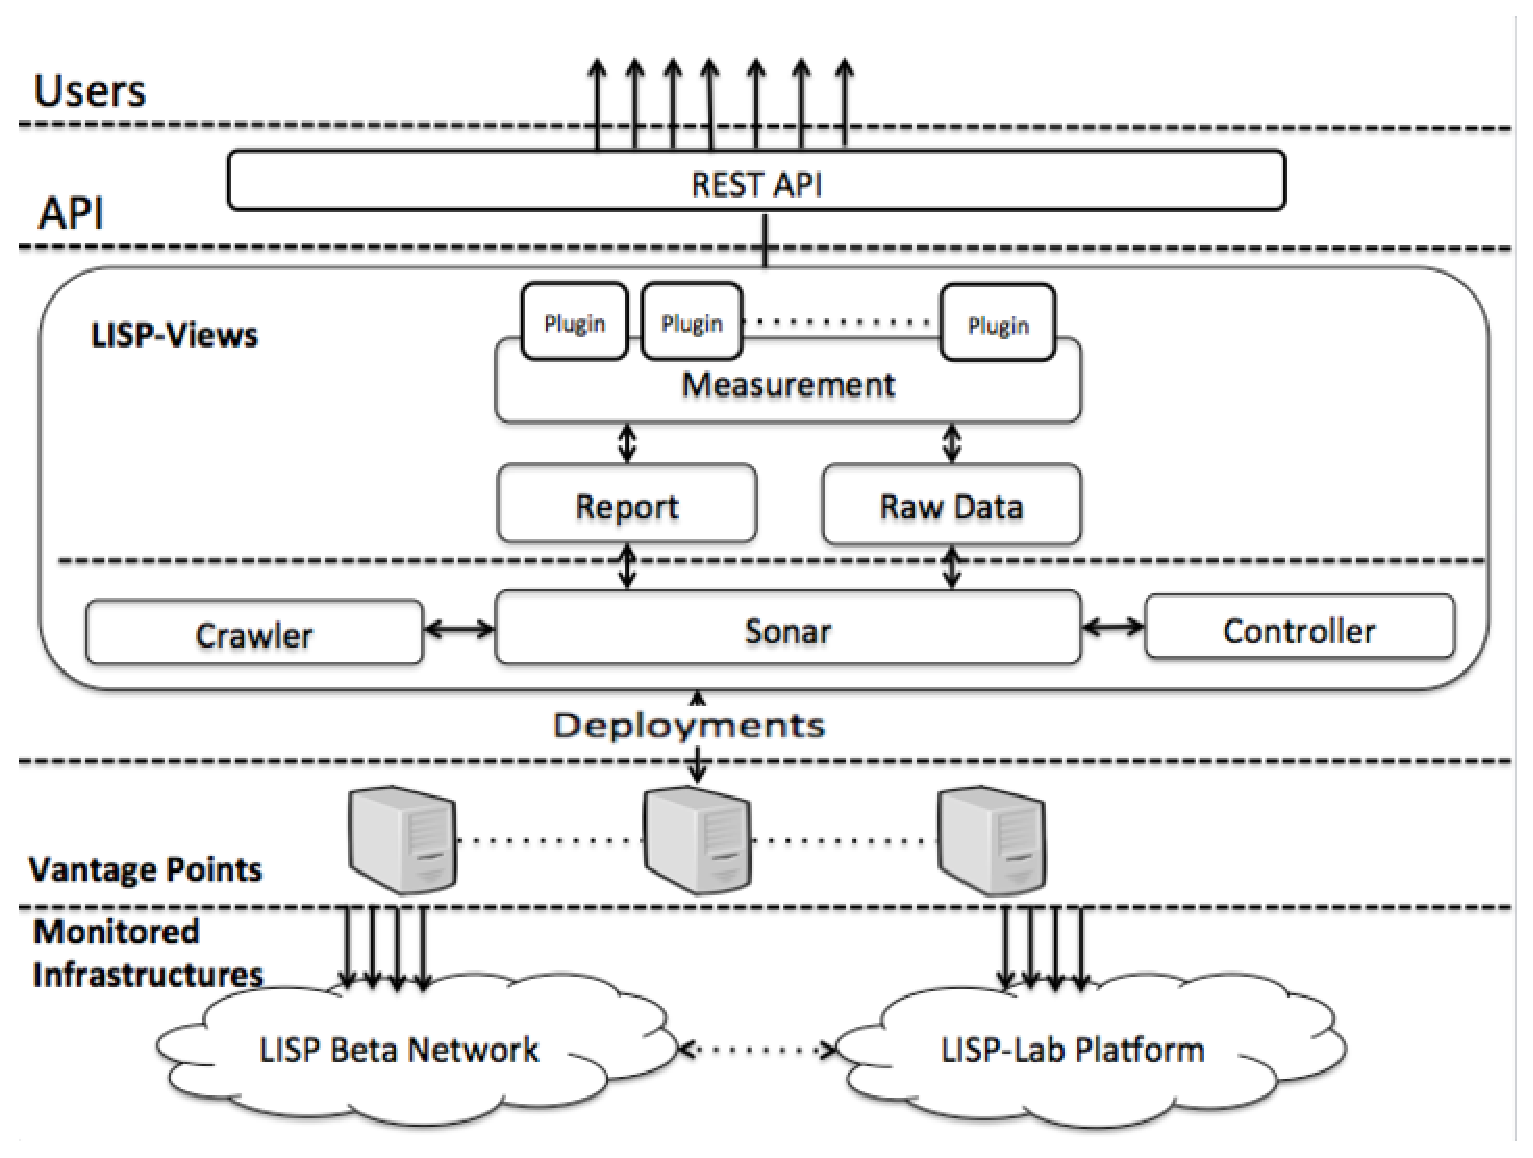
\includegraphics[width=0.9\textwidth]{Pics/LISP-Views_Arch.eps}
     \caption{Monitoring Architecture}
     \label{monitoring_arch}
\end{figure}
%-< END FIGURE >--------------------------------------------------------------------

The architecture of the proposed LISP-Views monitoring tools is depicted in Fig.~\ref{monitoring_arch}.  LISP-Views consists of several modules with different functions. The \emph{Measurement}, \emph{Report}, and \emph{Raw Data} modules are deployed on a centralized server while, the \emph{Crawler}, \emph{Sonar}, and \emph{Controller} modules can be deployed on several different \emph{VPs}.  As for now, LISP-Views is just deployed on one VP in Paris, France, where the monitor is developed and the centralized module is deployed. % Nevertheless, we are planing to implement the
The distributed version of LISP-Views is under development, for this reason, we will not discuss further how to deploy LISP-Views on multiple VPs. All the modules are implemented in \emph{Python} and described as follows:

\textbf{Sonar module}: the main module with two functions:
\begin{enumerate*}
   \item sending the LISP encapsulated Map-Requests and receiving the Map-Replies to/from all the existing MRs based on the standard~\cite{rfc6830};
   \item storing the received information in \emph{Report} and \emph{Raw Data} with different purposes.
\end{enumerate*}

The IP address that \emph{Sonar} uses to query to MRs is selected  either from the output of \emph{Crawler}, or from the recorded information in the previously produced \emph{Report}. The reasons are explained in the corresponding modules.

\textbf{Crawler module}: scans all the existing IPv4 addressing space using \emph{Sonar}.  If the queried IP (e.g., 192.0.2.1) has no Map-Reply, \emph{Crawler} increments the IP by one as the next queried IP (i.e., 192.0.2.2) and lets \emph{Sonar} send the Map-Request. If \emph{Sonar} obtains Negative or LISP Map-Reply, since the Reply contains a prefix (mentioned in Sec.~\ref{sec:background_lisp}), \emph{Crawler} sets the next query to the first IP beyond the returned prefix.  For instance if the returned prefix is 192.0.2.0/25, the next queried IP is 192.0.2.128.  Scanning the whole IPv4 address space takes very long time, and is mainly caused by time wasted waiting for no Map-Reply.  Indeed, no Map-Reply means to wait 3 seconds, and the next queried IP is just increased by one, instead of skipping a block of IP addresses like in the case of Negative/LISP Map-Reply.

\textbf{Report module}: contains the collected EID-prefixes in a list, as well as a list of MRs that answered. As crawling the address space may take long time but we aim to obtain the status of MRs as frequently as possible, \emph{Sonar} sends Map-Requests for the EIDs recorded in \emph{Report} only to MRs that have previously responded. Thus, it decreases the possibility to receive no Map-Reply, so that to get LISP status within a shorter time.

\textbf{Raw Data module}: contains all the detailed information of Map-Replies for each MR, such as Map-Reply type, RLOCs, required EID-Prefix, Round Trip Time (RTT) and the returned source for each round specify with $Time Stamp$ (regardless the source of \emph{Sonar}).  So, it can be used to perform thorough performance analysis of MDS. Moreover, since the \emph{Raw Data} is stored according to the MR, it is possible to track the performance of the MRs individually.

\textbf{Measurement module}: provides the composition of requested measurements (i.e., select different measurement plug-ins) based on the analysis of \emph{Raw Data} and \emph{Report}.

\textbf{REST API}: is connected to \emph{Measurement module} so that the users can launch a custom experiment by setting the experiment time, the monitored MRs, and obtain the different aspects of LISP status.  We are currently implementing the REST API, so the results of measurements presented here were obtained via the command lines.

\textbf{Controller module}: synchronizes all the modules in LISP-Views and also specifies the start and stop time of producing both \emph{Report} and \emph{Raw Data}. The interval of generating \emph{Report} and \emph{Raw Data} can be changed according to the hardware processing capability. However, since the inconsistency between MRs exits, the interval of producing Report and Raw Data for every MR differs from each other. Thus, the interval set in Control module should cover the slowest MR. 


%-< SECTION >--------------------------------------------------------------------
\section{LISP-Views Validation}
\label{sec:lispviews_evaluation}


%-< SUBSECTION >--------------------------------------------------------------------
\subsection{Methodology}
\label{sec:lispviews_evaluation_meth}
% \begin{itemize}[noitemsep,topsep=0pt]
%     \item Deployed LISP-Views on one VP, which is an xTR of LISP-Lab platform. 
%     \item Monitored during one month (from 0:00 September 4\textsuperscript{th} to midnight of October 4\textsuperscript{th} 2016).
%     \item The interval to produce \emph{Report} was 6 hours, and the interval to produce \emph{Raw Data} was 2 hours.
%     \item The analyzed results used in this chapter are collected from \emph{Raw Data} and \emph{Report}.
% \end{itemize}

In order to validate and evaluate the LISP-Views monitoring tool, we used raw data and report collected during one month (from 0:00 September 4\textsuperscript{th} to midnight of October 4\textsuperscript{th} 2016), by deploying LISP-Views on one VP, which is an \acrshort{xtr} of LISP-Lab platform.

The interval to produce reports was 6 hours, and the interval to produce raw data was 2 hours. Unfortunately, both MRs of LISP-Lab platform just responded to the Map-Requests at the first time and then stopped. They were not able to handle large number of queries, because the Map-Requests did fill the request queues, % which are not deployed in manner to sufficiently follow up the queries, 
resulting a drop in the MRs.  Per-se this is a success, because this bug was unknown, and the OpenLISP coders fixed the issue after our measurements.  All the results of evaluation used in this section only depend on the 6 working MRs of LISP Beta Network (3 in Europe, 1 in US and 2 in Asia) and the other 6 MRs were down at the moment of conducting the experiment. The aim of the work is to validate LISP-Views by assessing if it provides at least the same results as LISPmon.


%-< SUBSECTION >--------------------------------------------------------------------
\subsection{LISP-Views vs. LISPmon}
\label{sec:lispviews_evaluation_com}
% The comparison between LISPmon and LISP-Views.
% \begin{itemize}[noitemsep,topsep=0pt]
%     \item In most cases, LISP-Views receives around 20 LISP Map-Replies more than LISPmon.
%     \item LISP-Views detects that there were issues to normally receive LISP status, whereas
% LISPmon hides the reality.
%     \item LISP-Views finds that the change of overall Map-Replies is mainly affected by LISP Map-Replies.
%     \item LISP-Views observes that MRs may not work normally in some rounds but they are able to recover fast.
% \end{itemize}

%-< FIGURE >--------------------------------------------------------------------
\begin{figure}[!t]
     \centering
     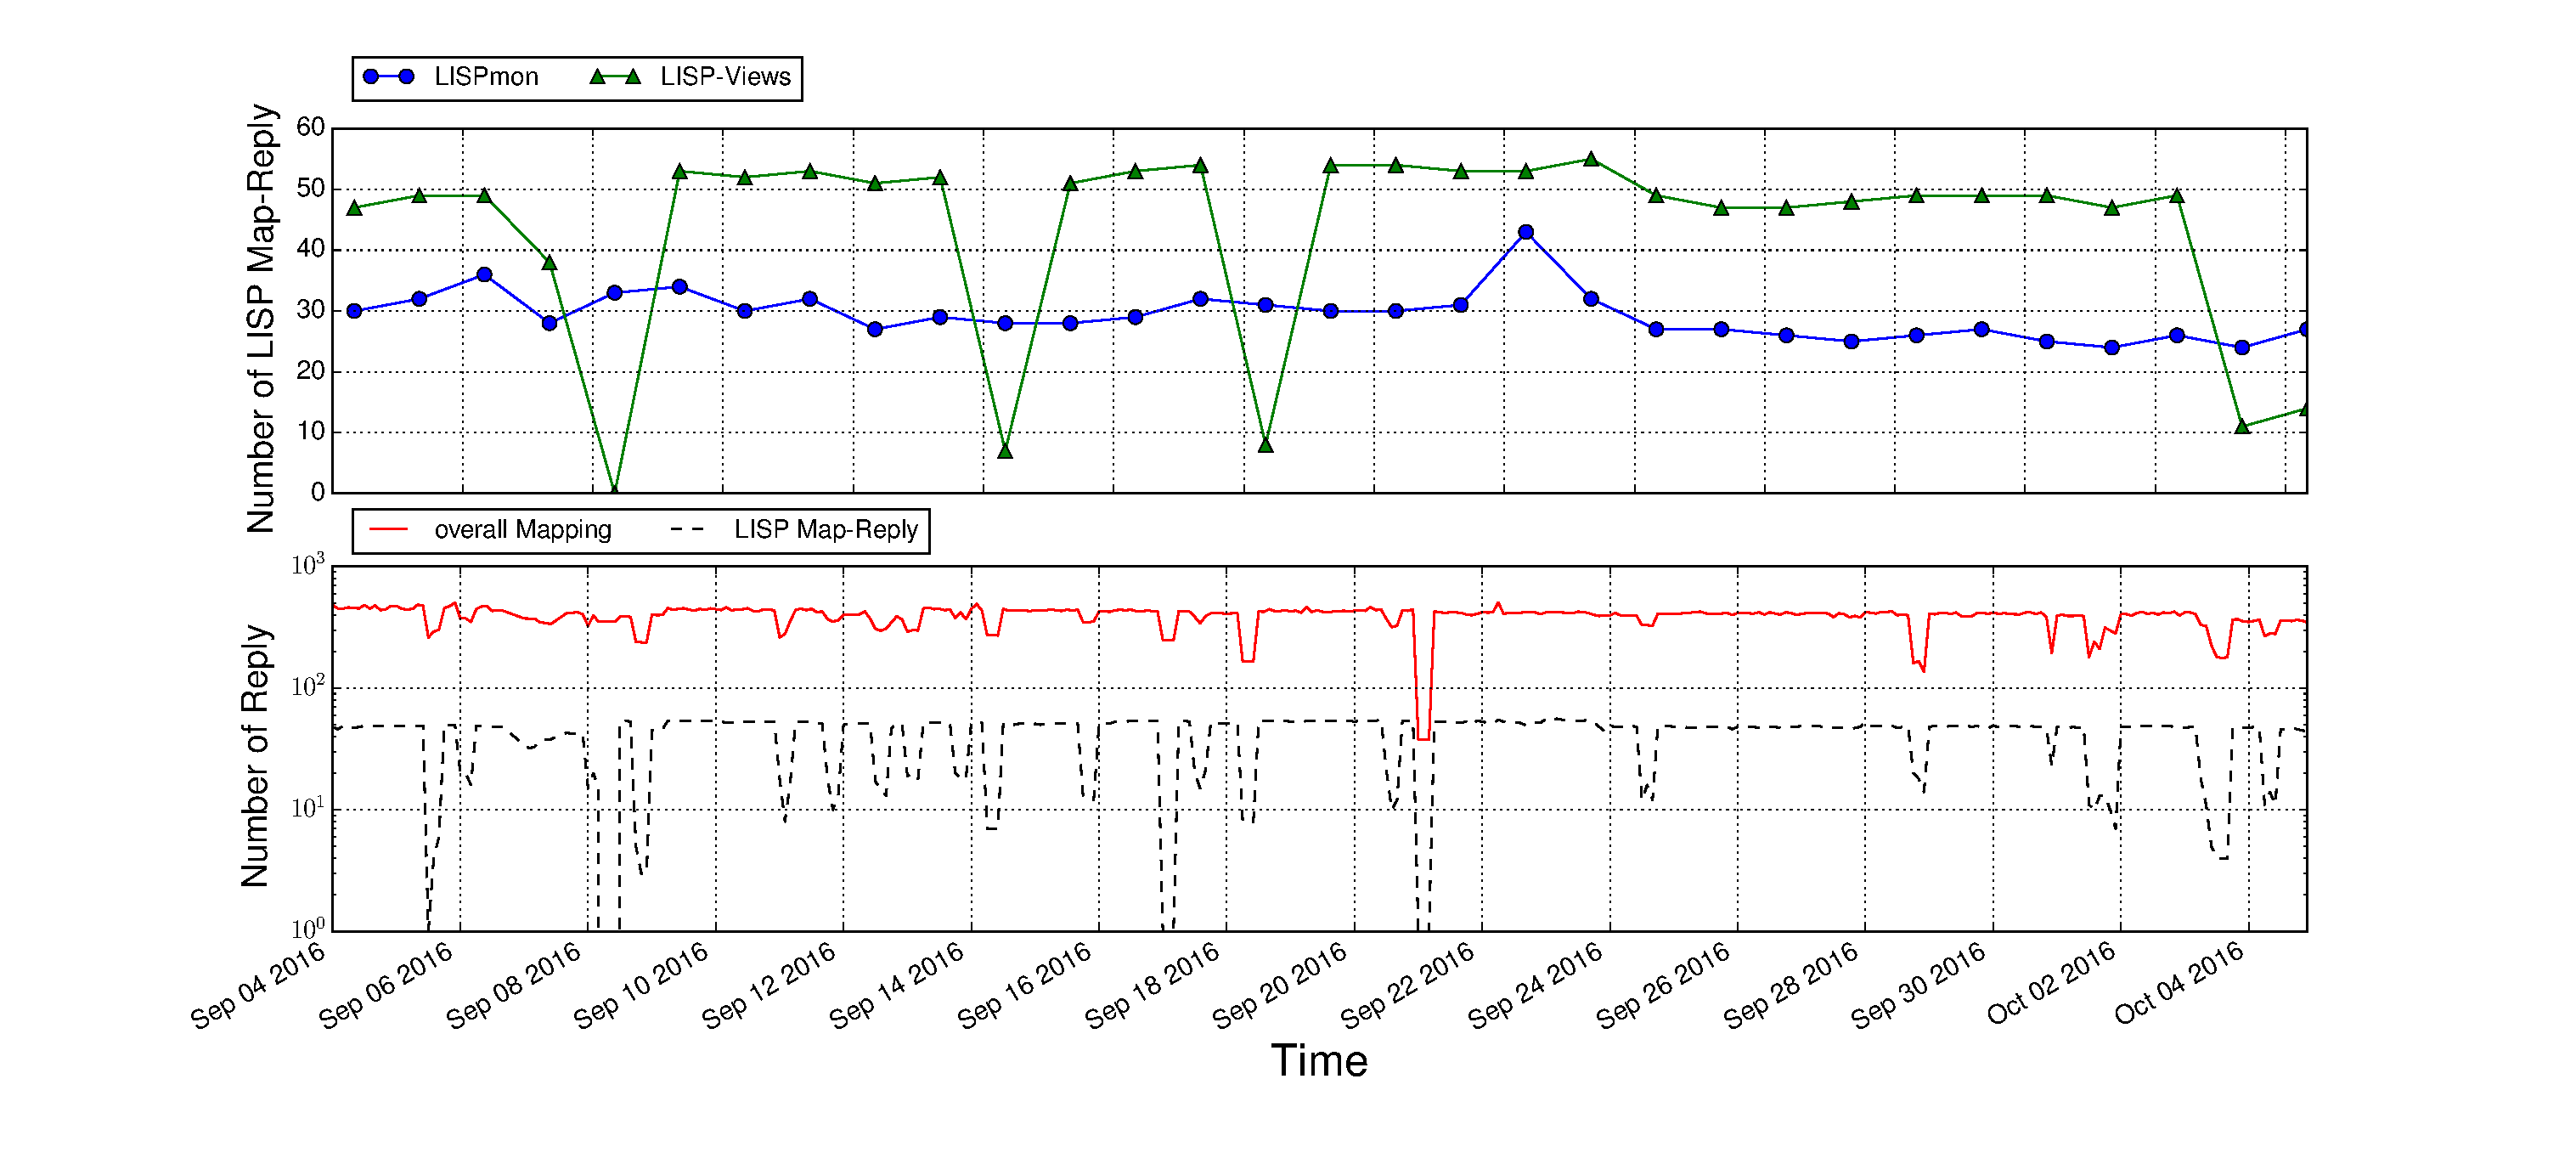
\includegraphics[width=1.1\textwidth]{Pics/LISPmon_comparison_all.eps}
     \caption{Comparison between LISPmon and LISP-Views. The upper
sub-figure shows the number of LISP Map-Reply from LISPmon generally at
7:00 and LISP-Views exactly at 8:00 over days. The bottom sub-figure
indicates the LISP Map-Reply and overall Mapping from LISP-Views over time with
an interval of 2 hours.}
     \label{lispmon_comparison}
\end{figure}
%-< END FIGURE >--------------------------------------------------------------------

In this section, we compare LISPmon and LISP-Views, so to assess if the information provided is comparable between the two monitoring platforms, hence validating LISP-Views.  As we indicated in Sec.~\ref{sec:lispviews_archi_motivation}, at any time LISPmon just queries one MR, on LISP Beta Network once per day and generally begins at 7:00~a.m.. The queried MR is changed sometimes when it has issues. LISP-Views, however, keeps sending Map-Requests to all the 6 MRs with an interval of 2 hours everyday, so to retrieve the actual real status of each MR.

Fig.~\ref{lispmon_comparison} shows the number of LISP Map-Replies received from LISPmon and LISP-Views over time. The upper sub-figure makes a comparison between the 2 monitors. The line with point is obtained from the daily LISPmon publications, indicating the number of LISP Map-Replies returned by one MR in an uncertain time monitoring round every day. To facilitate the comparison, we pick up the results from LISP-Views at 8:00 a.m., which is the nearest experimental round to LISPmon. As presented in the curve with triangle symbols, LISP-Views reflects the fact of a combination of the number of LISP Map-Reply containing the different EID-prefixes from all the MRs at a fixed experiment time. In most cases, LISP-Views receives around 20 LISP Map-Replies more than LISPmon, reflects the fact that the MRs are not coherent at any time due to the existence of convergence time for synchronizing the mapping information among them. The other 5 days, where LISP-Views receives very few LISP Map-Replies, show that there were issues to normally receive LISP status at that time, whereas LISPmon always presents a smoother trend but hides the reality.

The lack of stability can be better appreciated in the bottom sub-figure of Fig.~\ref{lispmon_comparison}. Such figure depicts the number of LISP Map-Reply (in dashed line) and the overall Mapping (LISP and Negative Map-Reply, in solid line) from LISP-Views for every 2 hours monitoring round during the whole experiment. Although the number of Map-Replies presented in the figure is still the combination of results from 6 MRs when the returned EID-prefixes are different, it shows that the MRs are not quite stable. Sometimes the MRs even provide 0 or less than 10 LISP Map-Replies, but in the next experiment round, the number is recovered. Besides, we evaluate the total number of successful queries every 2 hours. It also presents the behavior of instability, where it generally oscillates between 400 and 500, but it occasionally drops lower than 300. Both solid and dashed lines have almost same changing trend, indicating that the change of overall Map-Replies is mainly affected by LISP Map-Replies. Monitoring rounds where the number of LISP Map-Replies approaches 0 but where  Negative Map-Replies are still received indicate issues at the MRs, especially for answering the LISP Map-Reply.

%-< FIGURE >--------------------------------------------------------------------
\begin{figure}[!t]
        \centering
        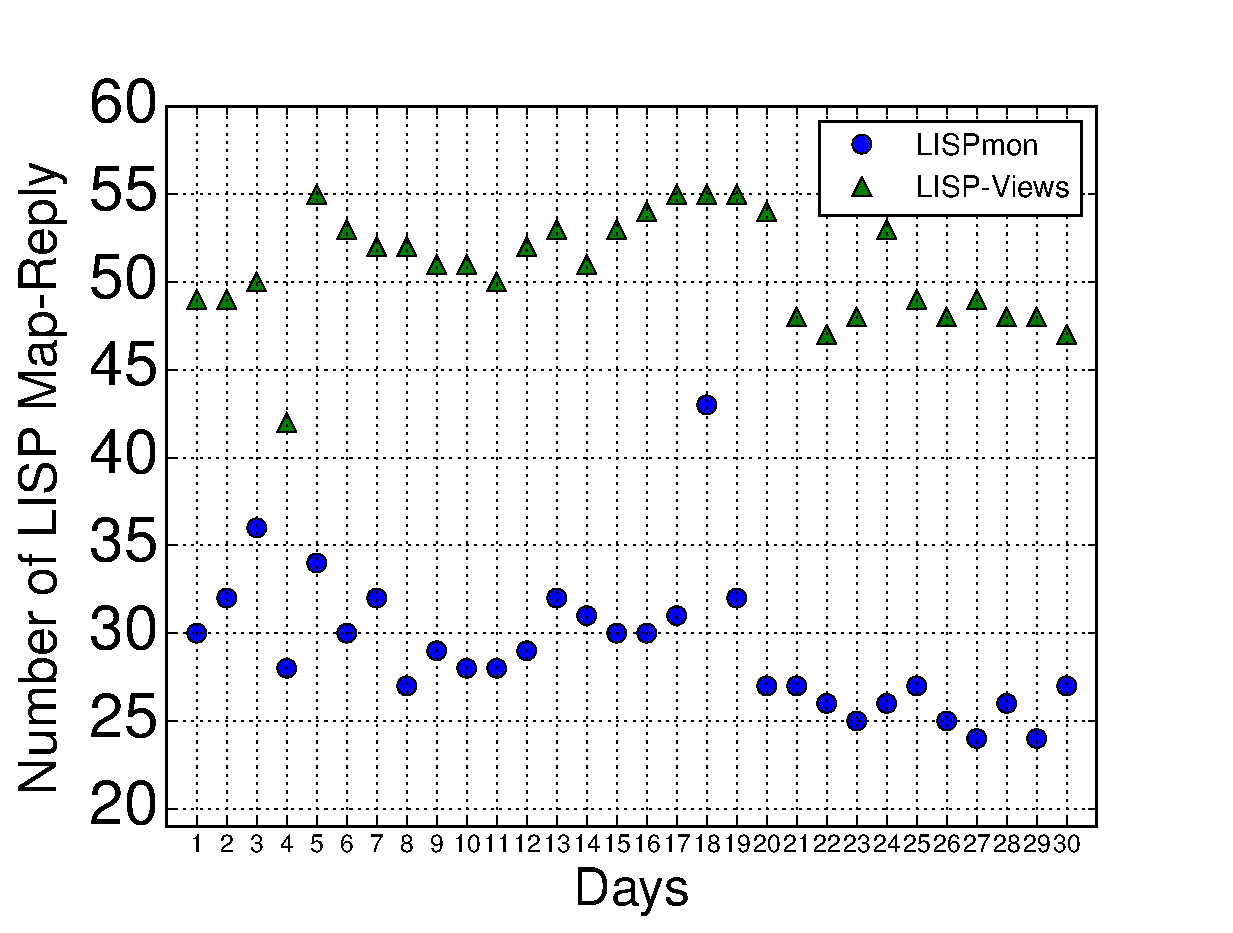
\includegraphics[width=0.7\textwidth]{Pics/LISPmon_comparison_day.eps}
        \caption{Comparison between the LISP Map-Reply of LISPmon and LISP-Views over days}
        \label{lispmon_comparison_day}
\end{figure}
%-< END FIGURE >--------------------------------------------------------------------

We compared the number of received LISP Map-Replies within a whole day between LISPmon and LISP-Views over 30 days. Shown in Fig.~\ref{lispmon_comparison_day}, as LISPmon only publishes one record each day, the number (represented by points) is exactly identical to those in Fig.~\ref{lispmon_comparison}. LISP-Views, however, provides a combination of LISP Map-Replies not only from all MRs but also from 12 monitoring rounds within one day. We observe that our monitor architecture receives more LISP Map-Replies than LISPmon in all days with a large difference. 83.3\% of the time LISP-Views receives more than 20 LISP Map-Replies. The maximum number of LISP Map-Replies that our proposed monitor obtains is 55, while the maximum value for LISPmon is 43. Differently from the upper sub-figure of Fig.~\ref{lispmon_comparison}, where LISP-Views occasionally receives nearly 0 LISP Map-Replies, the total number within a whole day is always more than 40, which illustrates that the MRs may not work normally in some rounds but they are able to recover fast. 

Since LISP-Views repeats querying simultaneously to every MRs, it is able to report on the status of each MR at anytime. It provides more complete mapping information compared to LISPmon and is also able to highlight sporadic issues with MRs.


%-< SECTION >--------------------------------------------------------------------
\section{Dissecting LISP with LISP-Views}
\label{sec:lispviews_results}
% This section presents several examples of how LISP-Views can be used to dissect LISP and obtain in-depth
% results.
% \begin{itemize}[noitemsep,topsep=0pt]
%     \item Used the same dataset in Sec.~\ref{sec:evaluation_meth}.
%     \item Reliability of each MR is inconsistent.
%     \item RTTs for getting mapping information from each MR is different.
%     \item CDF of RTT comparison between LISP and Negative Map-Reply.
%     \item Percentage of mapping source.
%     \item CDF of the number of RLOCs.
%     \item Demonstrate an example about one type of measurement captured on LISP-Views website.
% \end{itemize}

After validating LISP-Views in the previous section, this section presents several examples of how LISP-Views can be used to dissect LISP and obtain in-depth results. The experimental dataset used is the one in Sec.~\ref{sec:lispviews_evaluation_meth}.
% The methodology used is exactly same to Sec.~\ref{sec:evaluation_meth}.

%-< FIGURE >--------------------------------------------------------------------
\begin{figure}[!t]
        \centering
        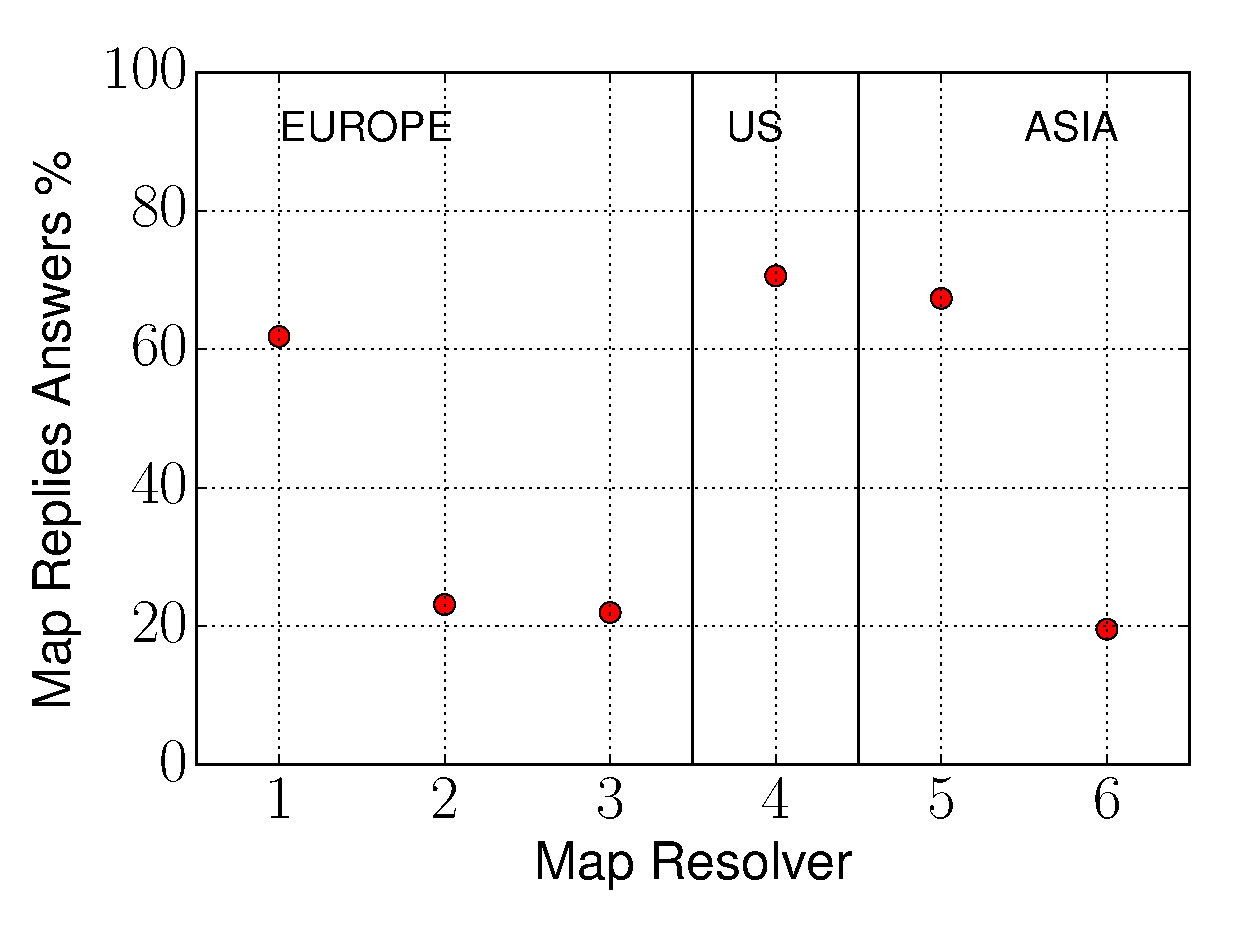
\includegraphics[width=0.7\textwidth]{Pics/Reliability.eps}
        \caption{Reliability of each MR}
        \label{MRs_reliability}
\end{figure}
%-< END FIGURE >--------------------------------------------------------------------
Fig.~\ref{MRs_reliability} shows the \emph{Reliability} of each MR during our
data collection, by calculating the percentage of successful queries over the
total number of Map-Requests. MR1, MR4, and MR5 give the highest
reliability values, which are more than 60\%. The lowest reliability values,
about 20\% are observed for MR2, MR3, and MR6. In general, the
reliability of each MR is different and low compared to the years of 2012 and
2013 presented in~\cite{coras2014performance}, which coincides with the fact
that there was a change of the MRs architecture on LISP Beta Network that year,
and an updated-software was tested on MRs as well.  The low value of
reliability is caused by MRs having an unstable behaviour, as shown in
Fig.~\ref{lispmon_comparison}, the number of Map-Reply changes heavily over
time, and especially the number of LISP Map-Reply sometimes drops to 0.

%-< FIGURE >--------------------------------------------------------------------
\begin{figure}[!t]
	\centering
	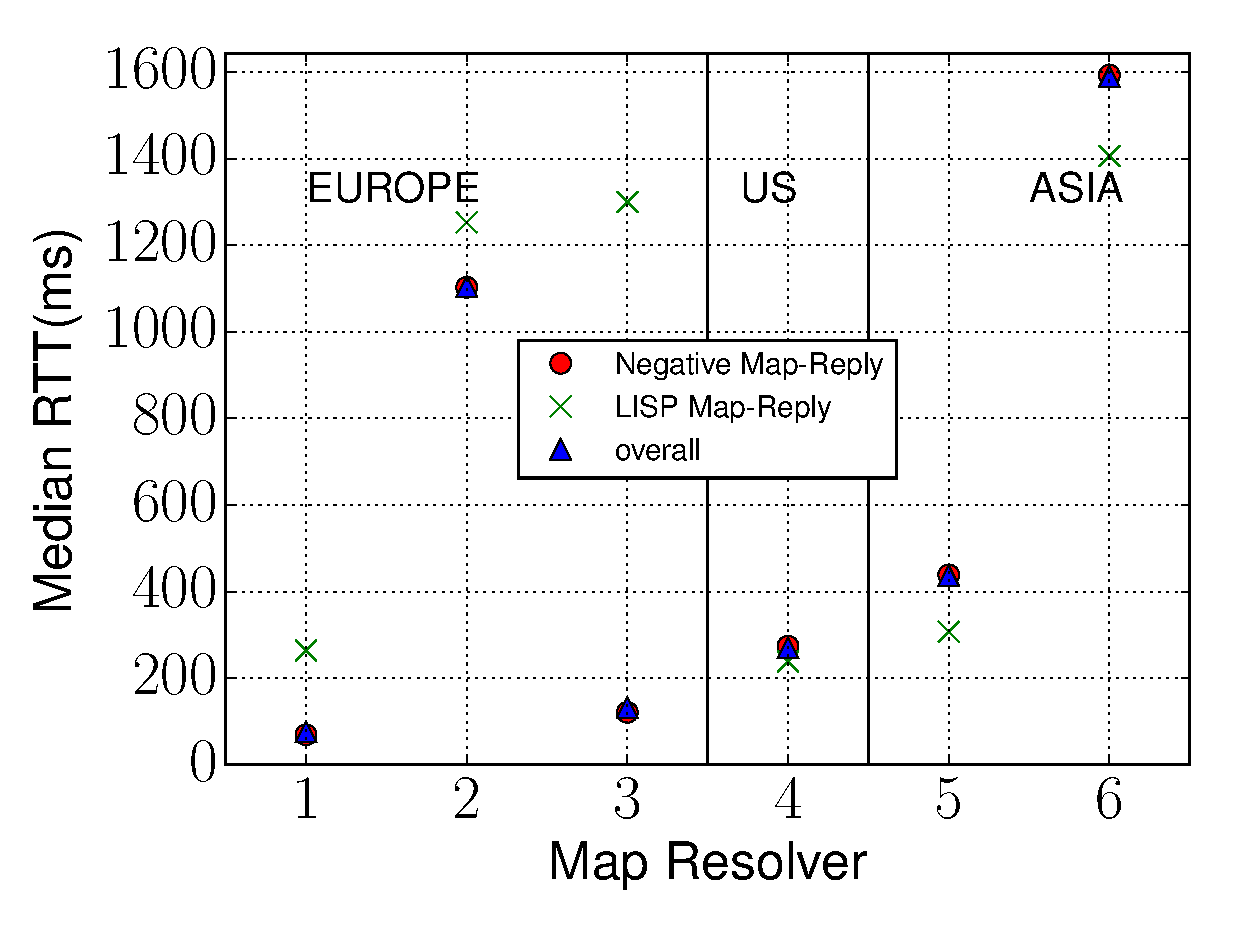
\includegraphics[width=0.7\textwidth]{Pics/median_of_RTT.eps}
	\caption{Median RTT per MR (In the most time, the Negative Map-Reply and overall are overlapped.)}
	\label{median_rtt_per_map-resolver}
\end{figure}
%-< END FIGURE >--------------------------------------------------------------------
In order to understand the behavior of each MR in terms of latency, we analyze
the median RTT obtained from our dataset. The RTT here refers to the Round Trip
Time from sending out the Map-Request until receiving the Map-Reply.
Fig.~\ref{median_rtt_per_map-resolver} shows that the best performance come
from MR1, MR3, MR4, and MR5; since the overall RTTs are much lower than
the others.  For MR3, the number of LISP Map-Replies is much higher than the
number of Negative Map-Replies, probably because its embedded Map-Server
registers less EID-prefixes hence requiring Map-Requests to be forwarded to a
remote MS. Then, the Map-Request is forwarded to the \acrshort{xtr}, where the remote MS
registers and the \acrshort{xtr} gives back the Map-Reply. Compared to the Negative
Map-Replies, which are normally returned by MR, LISP Map-Replies take longer
time, especially in this case. However, MR2 and MR6 present very high
latency, particularly for MR2 (located in Europe), but its RTT is even higher
than MR5, which is located in Asia. % It is mainly caused by a very high CPU usage of these two MRs preventing them sometimes to reply.  
If we focus on the RTT of LISP Map-Replies, only MR1, MR4, and MR5 provide the best
behavior, which coincides with the result of Fig.~\ref{MRs_reliability} on
reliability. The high RTTs of LISP Map-Replies are from the other 3 MRs,
where the median RTT is around 1300 ms, is caused by the failed queries.
Furthermore, it also explains why we can always receive the Negative
Map-Replies, but the number of LISP Map-Replies is sometimes quite low in
Fig.~\ref{lispmon_comparison}. Half of LISP Map-Replies are more than $1300 ms$
and partly even more than $3 s$. Since our measurement timeout is set to $3 s$,
it implies that some Map-Replies are dropped by our measurement unit.  As the
RTT of Negative Map-Replies is generally lower, we can receive more of them. This
phenomenon may be very biased by the VP location. % Thus, deploying LISP-Views on multiple VPs to get more reliability information is a paramount future work. 
In addition, Fig.~\ref{median_rtt_per_map-resolver} presents that the number of
Map-Replies returning from the MRs  located in Europe and US is indeed higher
than the number of Negative Map-Replies, which is expected. But both Asian MRs
return LISP Map-Replies faster than Negative Map-Replies. The reason of this 
observation is unclear and requires further exploration.

%-< FIGURE >--------------------------------------------------------------------
\begin{figure}[!t]
        \centering
        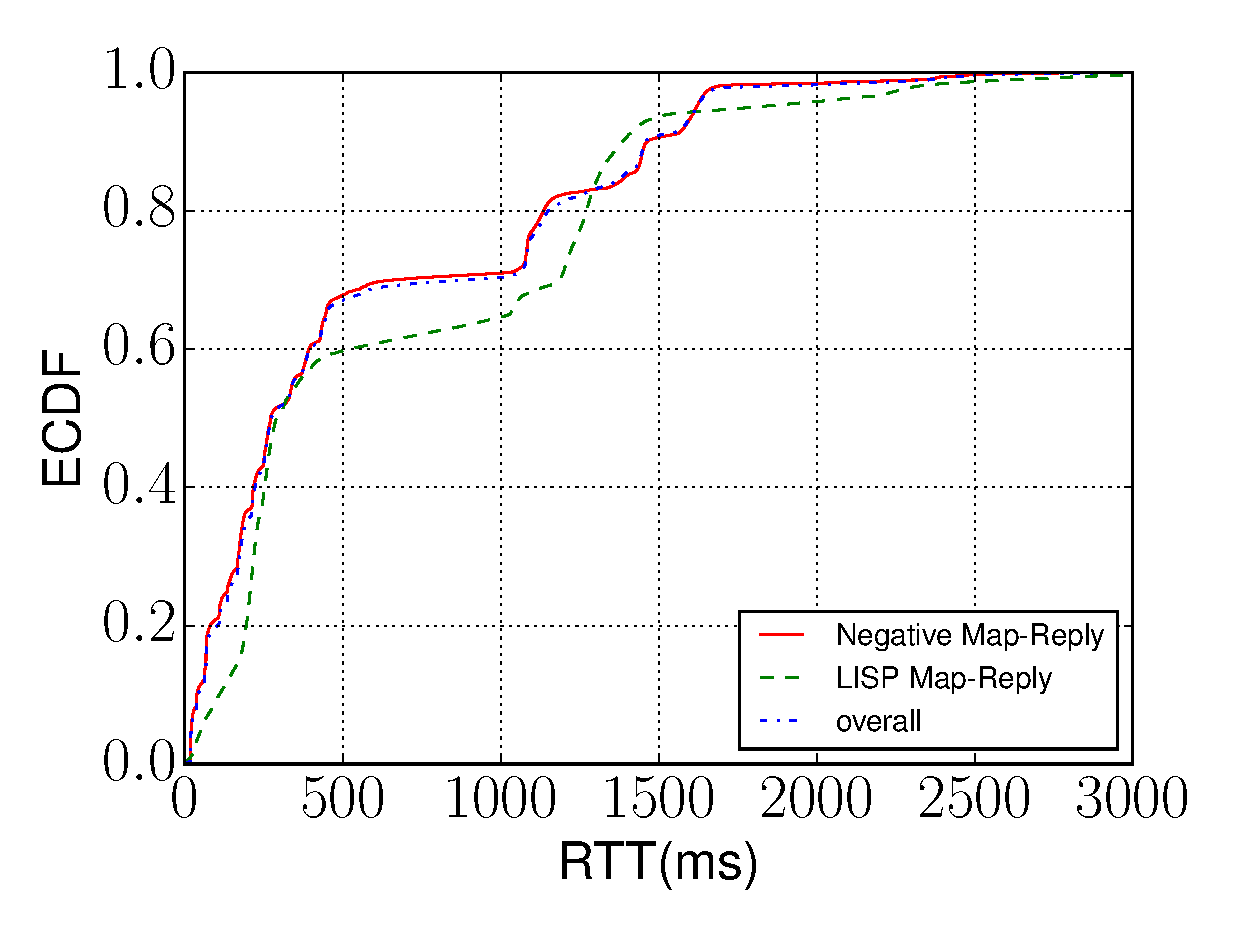
\includegraphics[width=0.7\textwidth]{Pics/ecdf_of_RTT.eps}
        \caption{CDF RTT comparison between LISP and Negative Map-Reply}
        \label{ecdf_rtt_lisp_negative}
\end{figure}
%-< END FIGURE >--------------------------------------------------------------------
We also calculate the Cumulative Distribution Function (CDF) of the
RTT for the 6 MRs. Fig.~\ref{ecdf_rtt_lisp_negative} provides the CDF of the
RTT for Negative, LISP, and overall Map-Replies. As indicated in
Sec.~\ref{sec:background_lisp}, the LISP \acrshort{mds} needs more time to solve a
complete mapping (LISP Map-Reply) than the Negative Map-Reply.  We observe that
the Negative Map-Reply is indeed faster than the LISP Map-Reply until the RTT
reaches 1000 ms, then the behavior changes, i.e., the LISP Map-Reply
sometimes becomes faster. What's more, we find that 67.03\% of RTTs within
500 ms, 70.33\% less than 1000 ms and 90.88\% don't exceed 1500 ms
for overall Map-Replies. In details, for the Negative Map-Reply, we found that
67.8\% of RTT values within 500 ms, for the LISP Map-Reply that 59.7\% of
RTT values less than 500 ms. This figure almost presents a bi-modal
distribution, where 500 ms is a peak and 1300 ms is another one. These two
high occurrences of RTTs are exactly the most two frequent latency in
Fig.~\ref{median_rtt_per_map-resolver}.


%-< TABLE >--------------------------------------------------------------------
\begin{table}[!t]
    \centering
    \caption{Percentage of Mapping Source}
    \label{tab:percentage_of_received_from}{
	\resizebox{0.6\textwidth}{!}{
        \begin{tabular}{c|c|c|c}
            \hline\hline
                Map-Reply Type     & Map Resolver   & xTR       & Other \\ \hline
                Negative Map-Reply &  98.79\%       &  -        &  1.21\% \\ \hline
                LISP Map-Reply     & 0.14\%         & 88.37\%   &  11.49\%  \\ \hline\hline
        \end{tabular}
        }}
\end{table}
%-< END TABLE >--------------------------------------------------------------------

The dataset obtained with our monitoring architecture also shows the
information about \emph{Mapping Source}. We explore the source answering the
Map-Replies according to different types (LISP or Negative). In the case of
LISP Map-Replies, we expect the source of replies to come either from one of
the ETRs or the queried MR. On the contrary, for Negative Map-Replies, replies
should just come from the queried MR. Tab.~\ref{tab:percentage_of_received_from} presents the percentage of
observations for the two types of Map-Replies. For the Negative Map-Reply,
98.79\% come from the queried MR and 1.21\% come from the other sources.
Further, the other sources are actually the other MRs without query and it
happens just for a fixed EID-Prefixes, i.e., if we send a Map-Request for one
of these EID-Prefixes to a dedicated MR, the Map-Reply always comes from a
fixed specific MR. As a conclusion, all the Negative Map-Replies are answered
by MRs. For the LISP Map-Reply, we observe that 0.14\% come from the queried
MR, 88.37\% come from one of their ETRs, but 11.49\% come from the other
sources in different locations. This unexpected behaviour needs further
investigation.

%-< FIGURE >--------------------------------------------------------------------
\begin{figure}[!t]
        \centering
        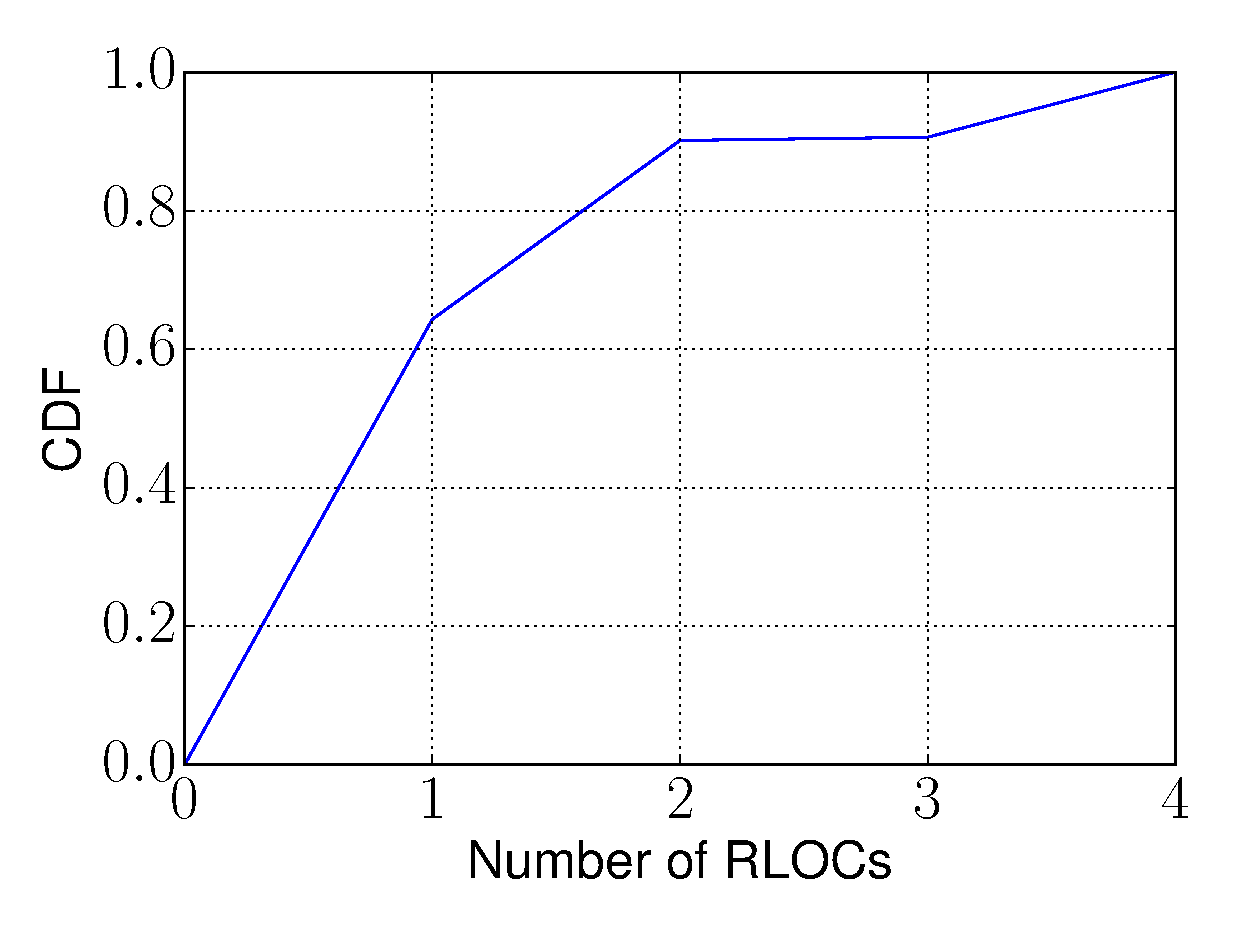
\includegraphics[width=0.7\textwidth]{Pics/CDF_of_RLOCs.eps}
        \caption{CDF of the number of RLOCs}
        \label{CDF_of_RLOCs}
\end{figure}
%-< END FIGURE >--------------------------------------------------------------------

%-< FIGURE >--------------------------------------------------------------------
\begin{figure}[ht]
        \centering
        \includegraphics[width=\linewidth]{Pics/Fig_on_LISPViews.eps}
        \caption{EIDs by Quantity of Associated RLOCs~\cite{lispviews}}
        \label{Fig_on_LISPViews}
\end{figure}
%-< END FIGURE >--------------------------------------------------------------------

The following type of measurement is the distribution of the size of RLOC set,
i.e., how many RLOCs are associated to one EID prefix on average. As
previously observed, the percentage of mappings using two or less RLOCs has
increased between 2010 and $2012$~\cite{lispCCR}. Fig.~\ref{CDF_of_RLOCs}
shows that this trend keeps going on, i.e., more mappings use fewer RLOCs and
the maximum number of RLOC is~4. An interesting point is that although LISP is a
good candidate to support the increasing multi-homing in Internet,
more than 60\% LISP users are not multi-homed and among them the majority
only has 2 RLOCs. Not only the number of RLOCs of each site does not significantly
change, but also the RLOCs themselves remains stable. We measured that the
stability reaches 99.8\% for all the dataset, i.e., once an
EID-prefix~--~to~--~RLOCs mapping is decided, it rarely changes. We have not found any mobile LISP sites.

All the aforementioned observations are based on the experiment made between
September and October 2016 as described in Sec.~\ref{sec:lispviews_evaluation_meth}.
Later LISP-Views detects that MR2 and MR6 in
Fig.~\ref{median_rtt_per_map-resolver} with very high overall RTTs are down,
and three new other MRs are up. After confirming with the operators of the LISP
Beta Network, these two MRs are indeed definitely down. The change of the
architecture of MRs also proves the accuracy of LISP-Views, while the LISPmon
presents a smooth change in its daily reports, hence hiding these facts. Since
February $2017$ LISP-Views publicly publishes preliminary daily reporting
online~\cite{lispviews}. % Development efforts are still ongoing to provide a complete and production-level website. 
Fig.~\ref{Fig_on_LISPViews} is a capture from the website, it is one type of measurement about the number of EID-prefix
quantified by the different size of RLOC set. The shown result is an union of
all MRs during a whole day, to present the most complete mapping information of
the actual LISP deployment. The line on the top indicates the number of LISP
Map-Replies, i.e., the Map-Replies with at least 1 RLOC, which coincides to
the results shown in Fig.~\ref{lispmon_comparison} and is mainly affected by
the EID-prefix with 1 RLOC.  Moreover, the composition of the different sizes
of RLOC set is also rather identical to the one in Fig.~\ref{CDF_of_RLOCs}. The
only difference is that in the previous dataset there is no EID-prefix with 3
RLOCs, while in the latest dataset it appears, but not very stable. In
addition, the line with 3 RLOCs is almost complementary to the line with 4
RLOCs. It is probably caused by one LISP-site that has 4 \acrshort{xtr}s but one being
always down, or the LISP-site having 4 interfaces on a same \acrshort{xtr} among which
one is down. Besides, the number of observed EIDs per day heavily drops two
times in the figure. Since the two valley don't drop to zero, we know that the
problem doesn't come directly from the \acrshort{mds}. Instead, the problem comes from
issues that occurred within the network of the LISP-Views server itself. This
observation highlights the need of distributing VPs.


%-< SECTION >--------------------------------------------------------------------
%\section{LISP-related Discussion and Conclusion}
\section{Summary}
\label{sec:lispviews_conclusion}
% \begin{itemize}[noitemsep,topsep=0pt]
%     \item Motivated by the only LISP monitor LISPmon
%     % \begin{itemize}[noitemsep,topsep=0pt]
%     %     \item Queries only from a specific MR on LISP Beta Network
%     %     \item Monitors on one VP
%     %     \item Records just once per day
%     %     \item Publishes results daily
%     % \end{itemize}
%     \item LISP-Views monitors LISP status as user-defined
%     % \begin{itemize}[noitemsep,topsep=0pt]
%     %     \item Queries from all working MRs on both LISP testbeds
%     %     \item Monitors on multiple VPs
%     %     \item Continuously records in a day
%     %     \item Obtains the measurement results on various aspects
%     % \end{itemize}
%     \item LISP-Views provides more information
%     % \begin{itemize}[noitemsep,topsep=0pt]
%     %     \item LISP Map-Replies change a lot even within one day
%     %     \item LISP MRs are not consistent
%     % \end{itemize}
%     \item Further work
%     \begin{itemize}[noitemsep,topsep=0pt]
%         \item Implement a REST API
%         \item Deployment on multiple VPs
%         \item Test IPv6 behavior
%     \end{itemize}
% \end{itemize}

Very little is known about the behavior of LISP in operational environments and it still lacks of troubleshooting tools. Motivated by the only LISP monitor deployed so far, named LISPmon, which records the current LISP status only from a specific MR just once per day, we propose a more dynamic LISP monitoring architecture, namely LISP-Views, so to deepen the understandings on LISP and to ease day-to-day operations and troubleshooting. As LISP-Views aims at being deployed in large scale and dynamic networks, we make a comparison with LISPmon to validate the former one by comparing their behavior during one full month.

It demonstrates that LISP-Views provides more information by discovering more mapping information from all MRs and more complete mapping information of each MR. Furthermore, with our proposed monitoring platform, more mapping system performance metrics such as reliability, latency, and configuration issues can be assessed, which helps for further LISP improvements. % LISP-Views
%*******************************************************************************
%****************************** Fifth Chapter *********************************
%*******************************************************************************

\chapter{Assessing LISP interworking performance through RIPE Atlas}
\label{cha:pxtr}
% **************************** Define Graphics Path **************************
\ifpdf
    \graphicspath{{Chapter6/Pics/Raster/}{Chapter6/Pics/PDF/}{Chapter6/}}
\else
    \graphicspath{{Chapter6/Pics/Vector/}{Chapter6/}}
\fi

%-< ABSTRACT >--------------------------------------------------------------------
% LISP is currently under standardization in IETF and is deployed in the wild at the same time, thanks to two testbeds: the LISP Beta Network and the LISP-Lab project. 
Thanks to two testbeds: the LISP Beta Network and the LISP-Lab project, LISP is gradually deployed in the wild. The interworking mechanism is proposed to ensure the communication between LISP-speaking sites and legacy Internet. % The performance of LISP interworking with legacy Internet is of paramount importance to promote the adoption of LISP in future Internet. 
Although LISP has been evaluated in terms of scalability~\cite{lispCCR}, stability~\cite{yue2016stability}, LISP evolution~\cite{li2017lisp}, and delay resolving the bindings between EIDs and RLOCs (\cite{lispCCR}, \cite{coras2014performance}), LISP was never analyzed from the aspect of the interworking with the legacy Internet at large scale. This dissertation fills this gap by providing a latency evaluation and routing path measurement about LISP interworking mechanism. The work is based on two experiments (one is conducted in 2015, the other one is in 2016) by using RIPE Atlas, which is the largest existing Internet measurement infrastructure for both IPv4 and IPv6. % Experimental results show that LISP introduces additional latency, especially for close destinations, but negligible for intercontinental long-distance destinations. The additional latency highly depends on the position of the new network element being in charge of the communication between LISP-sites and the legacy Internet. % Although LISP introduces some stretch, its performance is generally stable and its latency is not very high compared to natively forwarding without using LISP.

The experimental results confirm that the use of proxies to connect LISP and non-LISP sites introduce negative effects, which are important for the nearby destinations but can be ignored for the intercontinental long-distance destinations. It also shows that the selection of the proxy location is very important, since having them close either to the sources or to the destinations can decrease a lot the negative stretch. Although LISP introduces some overhead, the performance is quite stable for IPv4. However, the same conclusion does not hold for IPv6. We also observed that the interworking performance of the LISP-Lab platform is more reliable than the LISP Beta Network.

In the remainder, Sec.~\ref{subsec:atlas} and Sec.~\ref{subsec:alexa} introduce the necessary resources on which our experiment leveraged. Sec.~\ref{sec:pxtr_methodology} describes the methodology we used to conduct the experiment. Sec.~\ref{sec:pxtr_ping_v4_2015} and Sec.~\ref{sec:pxtr_ping_v4_2016} respectively present the IPv4 ping results obtained from 2015 and 2016. Sec.~\ref{sec:pxtr_ping_v6} shows the IPv6 ping results and Sec.~\ref{sec:pxtr_traceroute} indicates the traceroute results for both IPv4 and IPv6. % Finally, Sec.~\ref{sec:pxtr_conclusion} concludes the chapter. 
%-< ABSTRACT >--------------------------------------------------------------------

%\section{Introduction}
%\label{sec:pxtr_intro}
%To improve LISP and promote the deployment of LISP, implementations and large scale flexible experimental platforms are indispensable. At the moment of this writing, two LISP platforms are deployed world-wide. One is the experimental LISP Beta Network testbed~\cite{lispbeta} deployed in 2008, and the other one is LISP-Lab platform~\cite{lisplab} open to external experimenters since 2015. Both of them have all LISP-required network entities and have been inter-connected. Although LISP has been evaluated in terms of scalability~\cite{lispCCR}, stability~\cite{yue2016stability}, LISP evolution~\cite{li2017lisp}, and delay resolving the bindings between EIDs and RLOCs (\cite{lispCCR}, \cite{coras2014performance}), LISP is never analyzed from the aspect of the interworking with the legacy Internet at large scale. The performance of such interoperation is very important since it determines the deployment speed of LISP networks~\cite{feng2017locator}. Hence, it is necessary to assess how such platforms integrate with the legacy Internet, evaluate the performance, and offer realistic experience to improve the testbeds themselves and provide hints to move the LISP technology forward.
%
%We conduct two experiments: one spans 6 hours in 2015 and the other one lasts 15 days in 2016. The results confirm that the use of proxies to connect LISP and non-LISP sites introduce negative effects, which are important for the nearby destinations but can be ignored for the intercontinental long-distance destinations. It also shows that the selection of the proxy location is very important, since having them close either to the sources or to the destinations can decrease a lot the negative stretch. Although LISP introduces some overhead, the performance is quite stable for IPv4. However, the same conclusion does not hold for IPv6. Furthermore, we observe that the interworking performance of LISP-Lab is more reliable than LISP Beta Network.

%-< SECTION >--------------------------------------------------------------------
\section{Experiment resources}
\subsection{RIPE Atlas}
\label{subsec:atlas}
% \begin{itemize}[noitemsep,topsep=0pt]
%     \item RIPE Atlas~\cite{atlas} is the largest Internet measurement infrastructure. 
%     \item Consists of probes and anchors.
%     \item Measure the state of Internet in real time through a set of tools.
%     \item Probes and anchors have built-in measurements.
%     \item User can define the measurements through its provided API.
% \end{itemize}
%-< FIGURE >--------------------------------------------------------------------
\begin{figure}[!t]
	\centering
	\includegraphics[width=0.6\textwidth]{Pics/Atlas_probes_deployment.eps}
	\caption{Deployment of probes on RIPE Atlas in 2017}
	\label{Atlas_probes_deployment}
\end{figure}
%-< END FIGURE >--------------------------------------------------------------------

RIPE Atlas~\cite{atlas} is the largest Internet measurement infrastructure, consisting of a global network of more than 9000 probes all over the world that measure Internet connectivity, reachability, and provide an understanding of the state of the Internet in real time. The deployment of worldwide probes is shown in Fig.~\ref{Atlas_probes_deployment}. From early 2013, the hardware of the probe is a modified TP-Link wireless router (model TL-MR 3020) with a small USB thumb drive in it, but this probe does not support WiFi. Atlas also has more than 200 worldwide anchors, which are enhanced probes, offering more process capacity and sufficient bandwidth to support the larger number of measurements. Thus, the anchors are normally more stable, and can be used as reference. All the probes and anchors whenever are set up, they automatically start executing a set of pre-defined measurements, called built-in measurements. The set of built-in measurements contain \emph{ping}, \emph{traceroute}, \emph{DNS}, \emph{SSL} and some \emph{HTTP} requests, mostly towards well-known targets such as DNS root servers, but also towards some of the RIPE Atlas infrastructure components. Besides, the probes and anchors also provide the user-defined active measurements with the same measurement types. Volunteers all over the world host these small hardware devices to actively measure Internet performance. To avoid malicious attacks, credits are required to launch experiments and the amount of required credits varies according to experiment types. In addition, the maximum allowed number of measurements towards the same target is 10. RIPE Atlas provides a set of RESTful API with which experiment campaign parameters (e.g.,type of measurement, query source and destination, the duration and interval of experiment etc.) are passed to probes and measurement traces can be retrieved. Based on the available API, one can schedule experiment campaign in an automatic manner.

\subsection{Alexa}
\label{subsec:alexa}
Alexa~\cite{alexa}~\cite{alexatop} is a website created by Amazon which provides commercial web traffic data, global rankings, and other information on 30 million websites. The analytic such as website rankings is based on the data collected by a toolbar developed by Alexa and installed within users web browser. The toolbar  
provides functions such as popup blocker, a search engine,etc. In early 2015, Alexa stated that there had been 10 million downloads of the toolbar.
Alexa ranks sites based primarily on tracking a sample set of Internet traffic—users of its toolbar for the Internet Explorer, Firefox and Google Chrome web browsers. Due to its huge sampling space, the website ranking that it published is widely used to evaluation the popularity of websites.


%-< SECTION >--------------------------------------------------------------------
\section{Measurement Methodology}
\label{sec:pxtr_methodology}
% Two experiments have been conducted.
The mechanism of LISP interworking is presented in Sec.\ref{sec:background_Interworking} and Coras et Al.~\cite{coras2014performance} describe how the use of PxTRs introduces a stretch in the path between LISP and non-LISP networks. Thus, it is necessary to conduct a large scale experiment in the real world to quantify this overhead. The objective is to answer three questions through such an experiment: how much is the negative impact? Under which conditions such stretch has an important impact on the performance? Conversely, under which situation such overhead is so small that it can be ignored? The follows describe how we conduct our experiments.

%-< SECTION >--------------------------------------------------------------------
\subsection{Dataset 2015}
\label{sec:pxtr_meth_2015}
% \begin{itemize}[noitemsep,topsep=0pt]
%     \item 4 probes ping to 50 IPv4 destinations
%     \item Interval: 10 minutes
%     \item Duration: 6 hours (on November 6\textsuperscript{th} 2015)
% \end{itemize}
As the purpose of our experiment campaign is to fully obtain the knowledge about the LISP interworking performance with legacy Internet, we deployed a probe (RIPE Atlas probe number is $\#22341$) with IPv4 and IPv6 address on the LISP-Lab platform inside an academic institute in Paris, France to conduct the LISP-enabled active measurements. For IPv4, it uses both PETR and PITR of LISP-Lab to communicate with the legacy Internet, and the connection between the xTR of probe and PxTR is via a MPLS VPN. However, the MPLS tunnel did not support IPv6 at that time. Thus, we configure the ITR of the LISP-Lab probe natively forward the packets towards the Internet core for IPv6 targets (i.e., PETR is not used for IPv6). As a result, the IPv6 packets outgoing from this probe are not encapsulated into LISP packets and natively forwarded in the traditional way, but the returned packets still pass through the PITR of LISP-Lab platform.

%-< TABLE >-----------------------------------------------------------------
\begin{table}[!tb]
	\centering
	\caption{Different configurations of probes in 2015}
	\label{Probes_config_2015}{
	\resizebox{0.6\textwidth}{!}{%
		\begin{tabular}{@{}c|c|c|c@{}}
			\hline\hline
			Name & using LISP & network type  & probe/anchor   \\ \hline
			LISP-Lab &  yes & academic & probe\\  \hline    
			mPlane &  no  & academic & probe     	\\  \hline     
			rmd &  no & industrial & probe     	\\  \hline 
			FranceIX &  no & industrial & anchor     	\\  \hline \hline               
		\end{tabular}
	}}
\end{table}
%-< END TABLE >-----------------------------------------------------------------

The mPlane probe (\#13842) resides in an academic network and uses the conventional routing. It allows to compare with non-LISP academic networks. While the rmd probe (\#16958) resides in industrial network and also uses the conventional routing. It is chosen in order to compare with non-LISP and non-academic networks. Further, a stable probe with much more measurement capacity is necessary as a reference with all other probes. To this end, the only anchor in Paris named FranceIX (\#6118) is selected. It resides in an IXP (Internet Exchange Point) network and does not use LISP. Thus, in this experiment, there are in total 4 probes used as sources to conduct the active measurements. Tab.~\ref{Probes_config_2015} summarizes the different probes.

We are now in a setup phase, where we start with a reduced number of destinations so to first setup the automated experiments. In this first experiment, the selected 4 probes ping to the top 50 Alexa sites every 10 minutes during 6 hours. However, from the experiment we find that there are 14 websites resolve to the same IPv4 addresses. We filtered them, so the assessment presented in Sec.~\ref{sec:pxtr_ping_v4_2015} are analyzed by the results of 36 top popular websites. With the collected dataset, we evaluate the various performances leveraged on \acrshort{rtt}.

%-< SECTION >--------------------------------------------------------------------
\subsection{Dataset 2016}
\label{sec:pxtr_meth_2016}
% \begin{itemize}[noitemsep,topsep=0pt]
%     \item 5 probes ping/traceroute to 500 IPv4 and 122 IPv6 destinations
%     \item Interval: 30 minutes for ping, 60 minutes for traceroute
%     \item Duration: 15 days (from December 15\textsuperscript{th} to 29\textsuperscript{th} 2016)
% \end{itemize}
The new experiment still leverages on the LISP-Lab probe and RIPE Atlas infrastructure, but provides the following new contributions:
\begin{itemize}[noitemsep,topsep=0pt]
    \item Add another LISP probe connected to the LISP Beta Network as experimental source, to compare LISP-Beta Network and LISP-Lab.
    \item Enlarge the number of destinations to the first 500 most popular websites on the Alexa ranking~\cite{alexa}.
    \item Consider the performance of IPv6 besides IPv4.
    \item Use \emph{traceroute}, in complement to latency measurements, in order to have a deeper understanding of the observed behavior.
    \item Extend the experimental span to 15 days so to study potential periodicity of traffic.
\end{itemize}

%-< FIGURE >--------------------------------------------------------------------
\begin{figure}[!t]
	\centering
	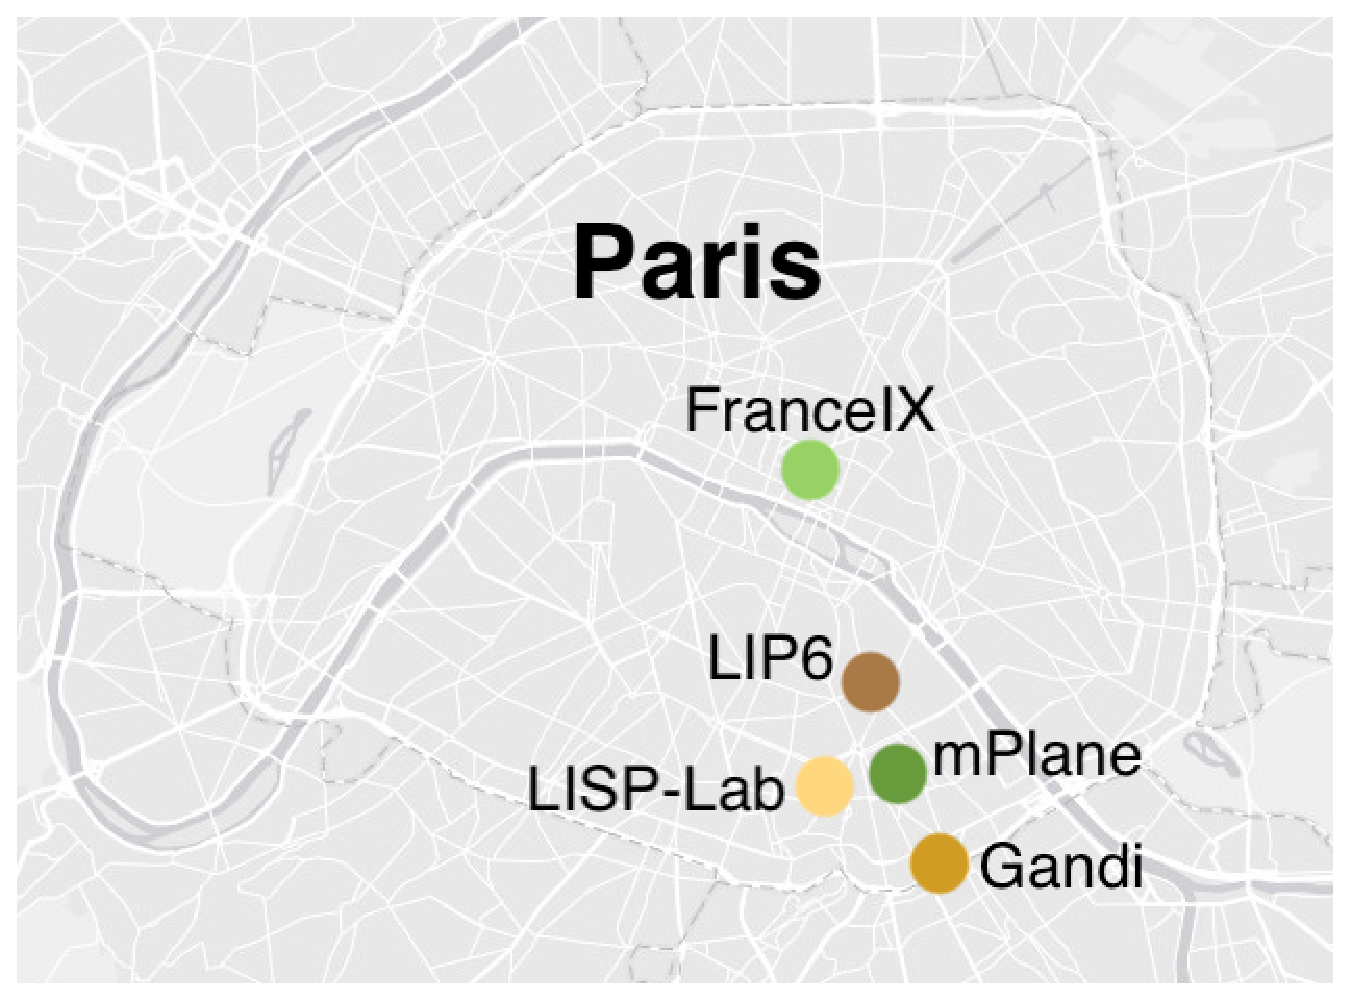
\includegraphics[width=0.6\textwidth]{Pics/Probes_loc.eps}
	\caption{Locations of probes and anchor in 2016}
	\label{Probes_location_2016}
\end{figure}
%-< END FIGURE >--------------------------------------------------------------------

%-< TABLE >-----------------------------------------------------------------
\begin{table}[!tb]
	\centering
	\caption{Location of LISP Beta Network PxTRs in 2016}
	\label{PxTR_loc_2016}{
	\resizebox{0.35\textwidth}{!}{%
		\begin{tabular}{@{}c|c|c@{}}
			\hline\hline
			Number & Continent  & Country   \\ \hline
			1 & Europe & Netherlands     	\\  \hline     
			2 & Europe & Denmark     	\\  \hline
			3 & Europe & Norway     	\\  \hline 
			4 & America & US     	\\  \hline      
			5 & America & US     	\\  \hline         
			6 & Asia & Japan     	\\  \hline  \hline                      
		\end{tabular}
	}}
\end{table}
%-< END TABLE >-----------------------------------------------------------------
% In order to ensure comprehensiveness and accuracy, we need some other probes geographically close to each other having both IPv4 and IPv6 address as comparative items. Ideally, they are connected through both the (non-) academic network provider and (non-) LISP platform. Thus, we selected 4 other probes located in Paris and their locations are shown in Fig.~\ref{Probes_location_2016}. 
The newly added LIP6 probe ($\#2403$) also connects to academic network behind both LISP Beta Network and LISP-Lab platform. When this probe communicates with the hosts in legacy Internet, it uses PETR of LISP-Lab by configuration, while return traffic goes through one of 6 PITRs of LISP Beta Network according to the BGP behavior. Depending on the BGP announcement to the legacy host, a different PITR is used. The more precise location of PITRs on LISP Beta Network is shown in Tab.~\ref{PxTR_loc_2016}: 3 are in Europe (Netherlands, Denmark and Norway), 2 are in US, and 1 is in Asia (Japan). Both LISP probes have a MPLS tunnel from their ITRs to the PETR at Lyon for IPv4, while for IPv6, the ITR of LIP6 probe is configured to use normal BGP routing to reach the PETR in Lyon (i.e., PETR is used but without MPLS VPN). The use of the MPLS tunnel IPv4 packets experience a shorter path compared to the IPv6 BGP-based one. Thus, theoretically the IPv4 packets sending from the LIP6 probe should arrive to PETR faster than those of IPv6. The configuration of two LISP probes are listed in Tab.~\ref{LISP_config}. 

%-< TABLE >-----------------------------------------------------------------
\begin{table}[!tb]
	\centering
	\caption{Configuration of two LISP probes in 2016}
	\label{LISP_config}{
	\resizebox{0.6\textwidth}{!}{%
		\begin{tabular}{@{}c|c|c@{}}
			\hline\hline
			Probe & PETR in Lyon  & PITR   \\ \hline
			LISP-Lab (IPv4) &  Via MPLS Tunnel & Lyon \\ 
			& & (Via MPLS Tunnel) 	\\  \hline      
			LIP6 (IPv4) &  Via MPLS Tunnel & LISP Beta Network     	\\  \hline     
			LISP-Lab (IPv6) &  not used  & Lyon     	\\  \hline     
			LIP6 for (IPv6) &  Via BGP Routing & LISP Beta Network     	\\  \hline \hline               
		\end{tabular}
	}}
\end{table}
%-< END TABLE >-----------------------------------------------------------------

Since the rmd probe is not configured with an IPv6 address, we replace it by the Gandi probe (\#3141), which also resides in an industrial network and also uses the conventional routing for both IPv4 and IPv6. % Although it is a little further to the LISP-Lab probe than the rmd probe, it is the nearest probe having both IPv4 and IPv6. 
As the mPlane probe and the FranceIX anchor satisfy all the requirements of this experiment, we still keep them as the reference. The locations of all the probes and anchor are shown in Fig.~\ref{Probes_location_2016}. Tab.~\ref{Probes_config_2016} shows the different configurations of probes.

%-< TABLE >-----------------------------------------------------------------
\begin{table}[!tb]
	\centering
	\caption{Different configurations of probes in 2016}
	\label{Probes_config_2016}{
	\resizebox{0.6\textwidth}{!}{%
		\begin{tabular}{@{}c|c|c|c@{}}
			\hline\hline
			Name & using LISP & network type  & probe/anchor   \\ \hline
			LISP-Lab &  yes & academic & probe\\  \hline
			LIP6 &  yes & academic & probe     	\\  \hline     
			mPlane &  no  & academic & probe     	\\  \hline     
			Gandi &  no & industrial & probe     	\\  \hline 
			FranceIX &  no & industrial & anchor     	\\  \hline \hline               
		\end{tabular}
	}}
\end{table}
%-< END TABLE >-----------------------------------------------------------------

What we care about is the delay performance and the path of LISP interworking with legacy Internet. Thus, we rely on the ping and traceroute tools provided by RIPE Atlas. As destinations of our measurements we selected the 500 most popular websites (according to worldwide website ranking provided by Alexa [24]), which reply to IPv4 ping and traceroute. Among them, 122 websites are configured with IPv6 address. Thus, in our experiment, 500 IPv4 and 122 IPv6 addresses are the destinations of ping and traceroute. We develop a Python script to schedule the experiment campaign by using the API provided by RIPE Atlas. The parameters of experiment campaign are as follows: the experiment campaign lasts 15 days (from December 15\textsuperscript{th} to 29\textsuperscript{th} 2016). The 5 chosen probes ping and traceroute to 500 IPv4 and 122 IPv6 addresses. The intervals of ping and traceroute measurements are respectively 30 minutes and 60 minutes. We want to evaluate LISP interworking performance as frequently as possible, but each probe sequentially launches 622 traceroute measurements, which last more than 30 minutes. To avoid the heavy traffic burden and guarantee that all the measurements in a same experimental round can be finished before next round, we set the sampling interval of traceroute at 60 minutes. As a summary, the results presented in this journal come from the following 4 experiment campaigns:
\begin{itemize}[noitemsep,topsep=0pt]
	\item 5 probes ping to 500 destinations during 15 days with an interval of 30 minutes (IPv4).
	\item 5 probes ping to 122 destinations during 15 days with an interval of 30 minutes (IPv6).
	\item 5 probes traceroute to 500 destinations during 15 days with an interval of 60 minutes (IPv4).
	\item 5 probes traceroute to 122 destinations during 15 days with an interval of 60 minutes (IPv6).
\end{itemize}

From the experiment, we find that some websites actually resolve to the same IPv4 (34 over 500) or IPv6 (47 over 122) addresses. Further, for some destinations, at least one probe (mainly the LIP6 probe) does not get any responses of \emph{ping} during the whole experiment (42 for IPv4 and 10 for IPv6). In this paper, we filtered the anycast destinations and only consider responding destinations. Thus, after cleaning the traces for the above reasons, all the results of \emph{ping} measurements used in the following subsections consists on the 5 chosen probes as the experimental sources and 424 IPv4 and 65 IPv6 responding addresses as the destinations. Differently from the ping measurements, for the \emph{traceroute} dataset, all the successful \emph{traceroute} responses from each probe are kept for further analysis.


 %-< SECTION >--------------------------------------------------------------------
\section{IPv4 Ping results from Dataset 2015}
\label{sec:pxtr_ping_v4_2015}
% \begin{itemize}[noitemsep,topsep=0pt]
%     \item CDF of average RTT between different probes
%     \item Correlation coefficient to FranceIX
%     \item Smallest mean and median RTT grouped by continent
%     \item Relative mean and median RTT clustered by continent
% \end{itemize}
%-< FIGURE >--------------------------------------------------------------------
    \begin{figure}[!t]
     	\centering
     	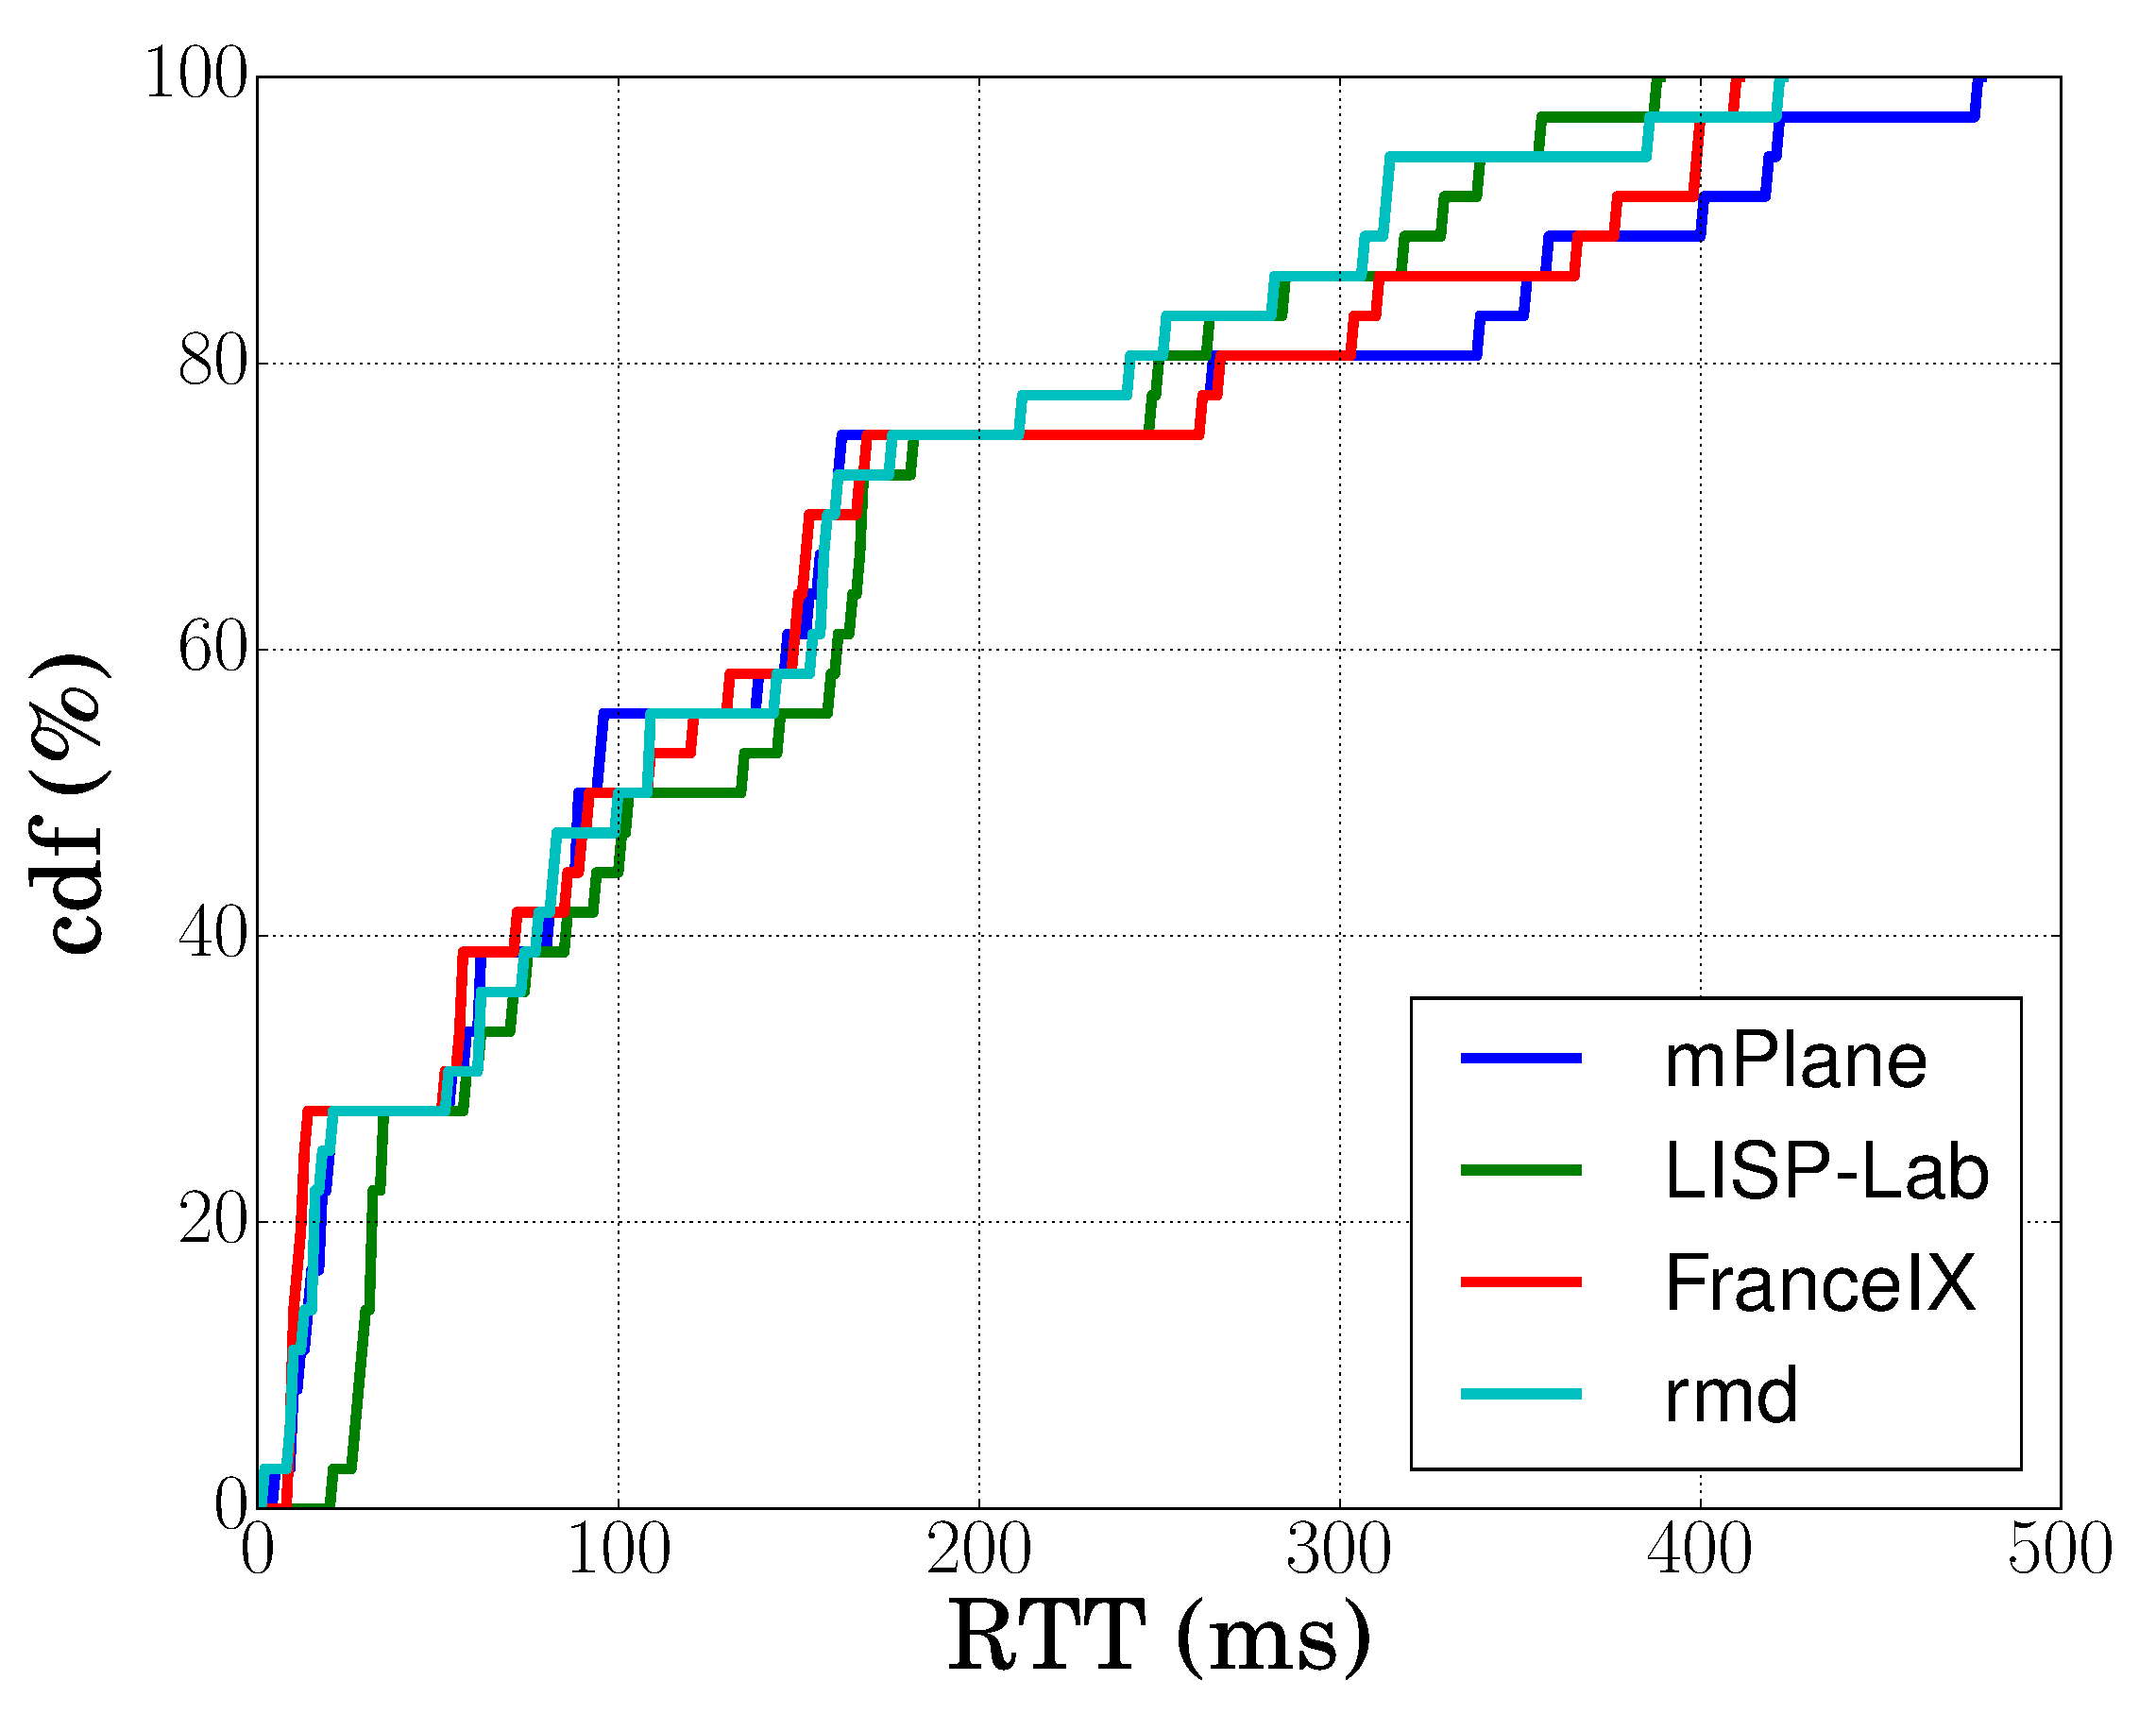
\includegraphics[width=0.6\textwidth]{Pics/2015/CDF_RTT_avg.eps}
     	\caption{CDF of average RTT between different probes from Dataset 2015}
     	\label{CDF_RTT_avg_v4_2015}
     \end{figure}
    %-< END FIGURE >-----------------------------------------------------------------
    
Fig.~\ref{CDF_RTT_avg_v4_2015} shows the cumulative distribution function (CDF) of average RTTs towards the selected 50 targets. Since the experimental destinations are located all over the world, the range of observed RTTs varies from few milliseconds (ms) to nearly five hundreds ms. When the RTT values are in the small range, especially when RTT is less than $50ms$, the latency from LISP-Lab probe is always higher than the three others and the difference is mainly around $10ms$. This latency difference is caused by the stretch introduced by the proxy technology (cf. Sec.\ref{sec:background_Interworking}), since every packet sent between LISP-Lab probe and the legacy Internet has to pass through the LISP-Lab PxTR, which is located in Lyon (approximately $400km$ away from the probe). As the RTT increases, actually the difference (surprisingly) decreases. When the RTT around $200ms$ is reached, all probes show basically the same RTT. Around such RTT values, the destinations concentrate in North America. Going further in the high range RTT values, i.e., more than $350ms$, when destinations are mainly located in Asia, the probe in the LISP-Lab domain actually shows the lowest RTT. Thus, it indicates that the network connection between the LISP-Lab PxTR to the (asian) intercontinental destinations has a better performance and the stretch delay from LISP-Lab probe to PxTR can be ignored. We wanted to use traceroute to further investigate the reasons, but it cannot be natively used at that moment, since the LISP-encapsulation prevents its correct function. We explored a new way to find out what happens for Dataset 2016, which is described in Sec.~\ref{sec:pxtr_traceroute}. 
    
We tried to quantify the percentage of times that one probe's RTT is the smallest compared to three others, since the destinations that the different probes contact to are exactly the same. The result shows that in $52.8\%$ of the time, FranceIX shows the smallest RTT to reach the destinations. It is normal that its RTTs are the smallest, since FranceIX is an Internet Exchange Point (IXP), hence well connected, and also acts as one of the anchors of RIPE Atlas, thus with a more powerful hardware. While, only in the $5.6\%$ of the cases, the LISP-Lab probe has the smallest RTT. In this small percentage the main contribution comes from Intercontinental destinations, i.e., when the RTT values belong to high range.
    
\begin{figure}[!t]
	\begin{minipage}[c]{.49\linewidth}
		\begin{center}
			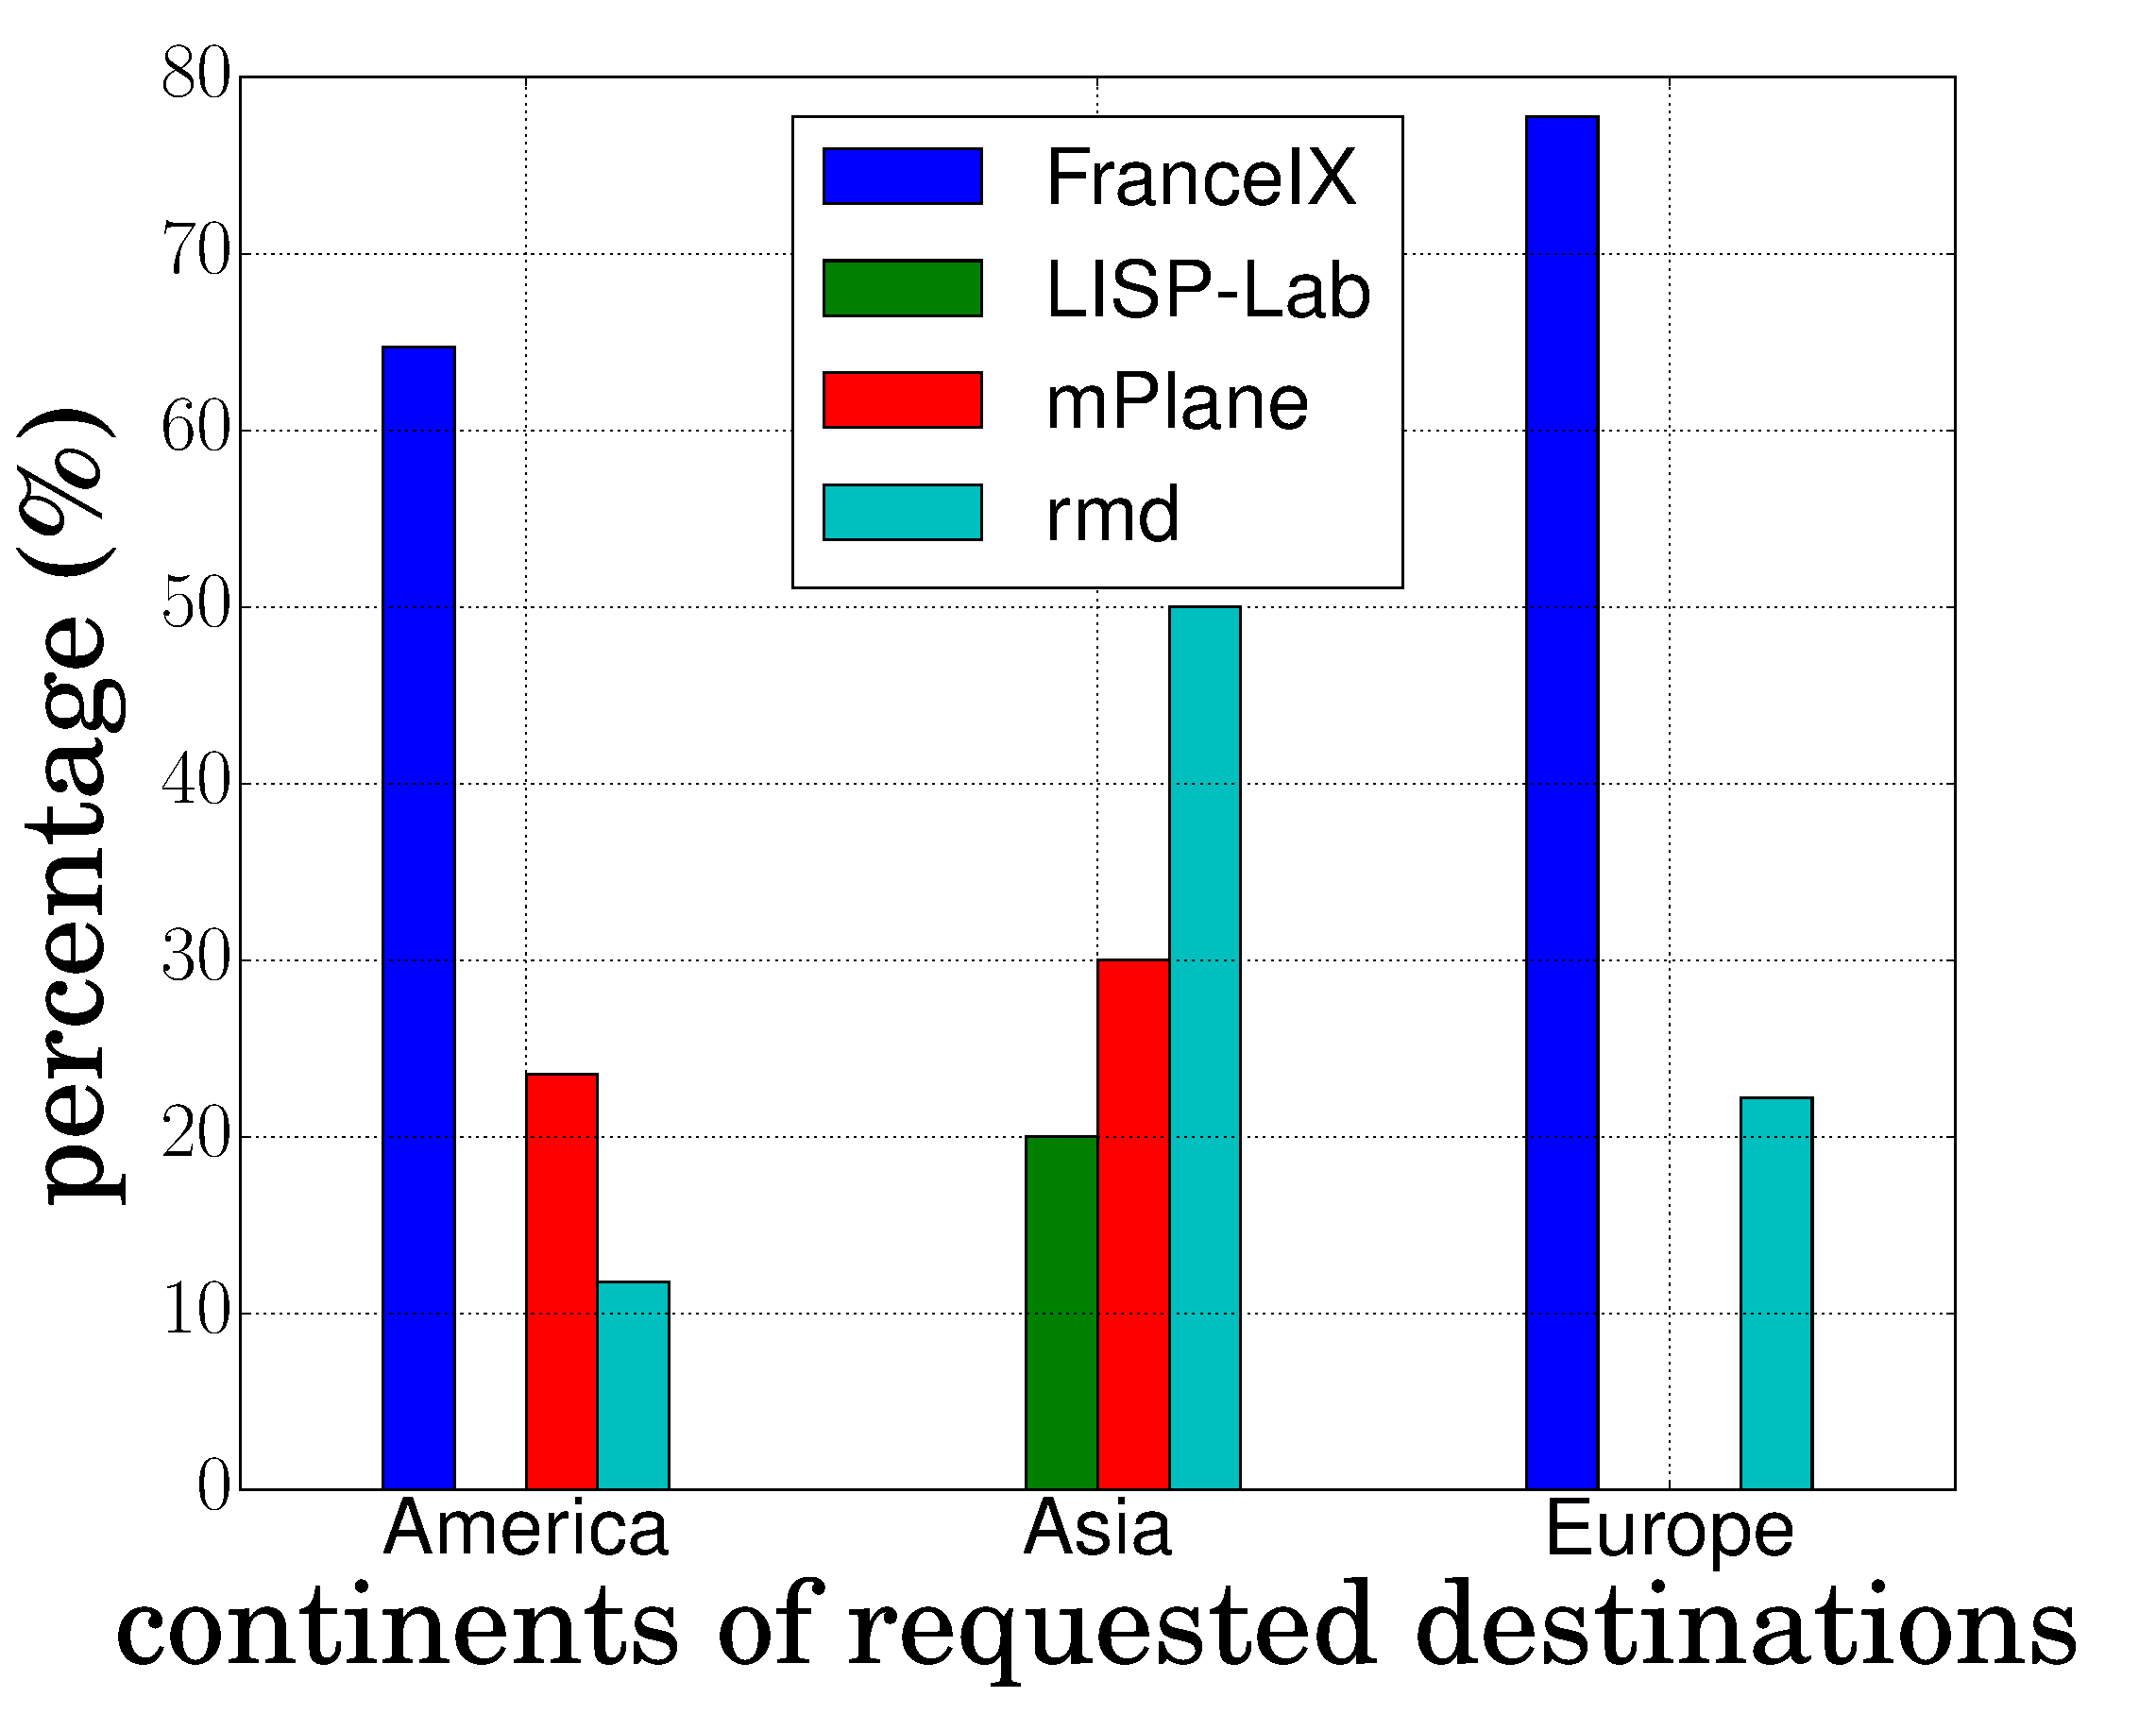
\includegraphics[width=.9\linewidth]{Pics/2015/4_probes_to_alexa_top50_proportion_mean_bar_geo.eps}
		\end{center}
	\end{minipage}
	\begin{minipage}[c]{.49\linewidth}
		\begin{center}
			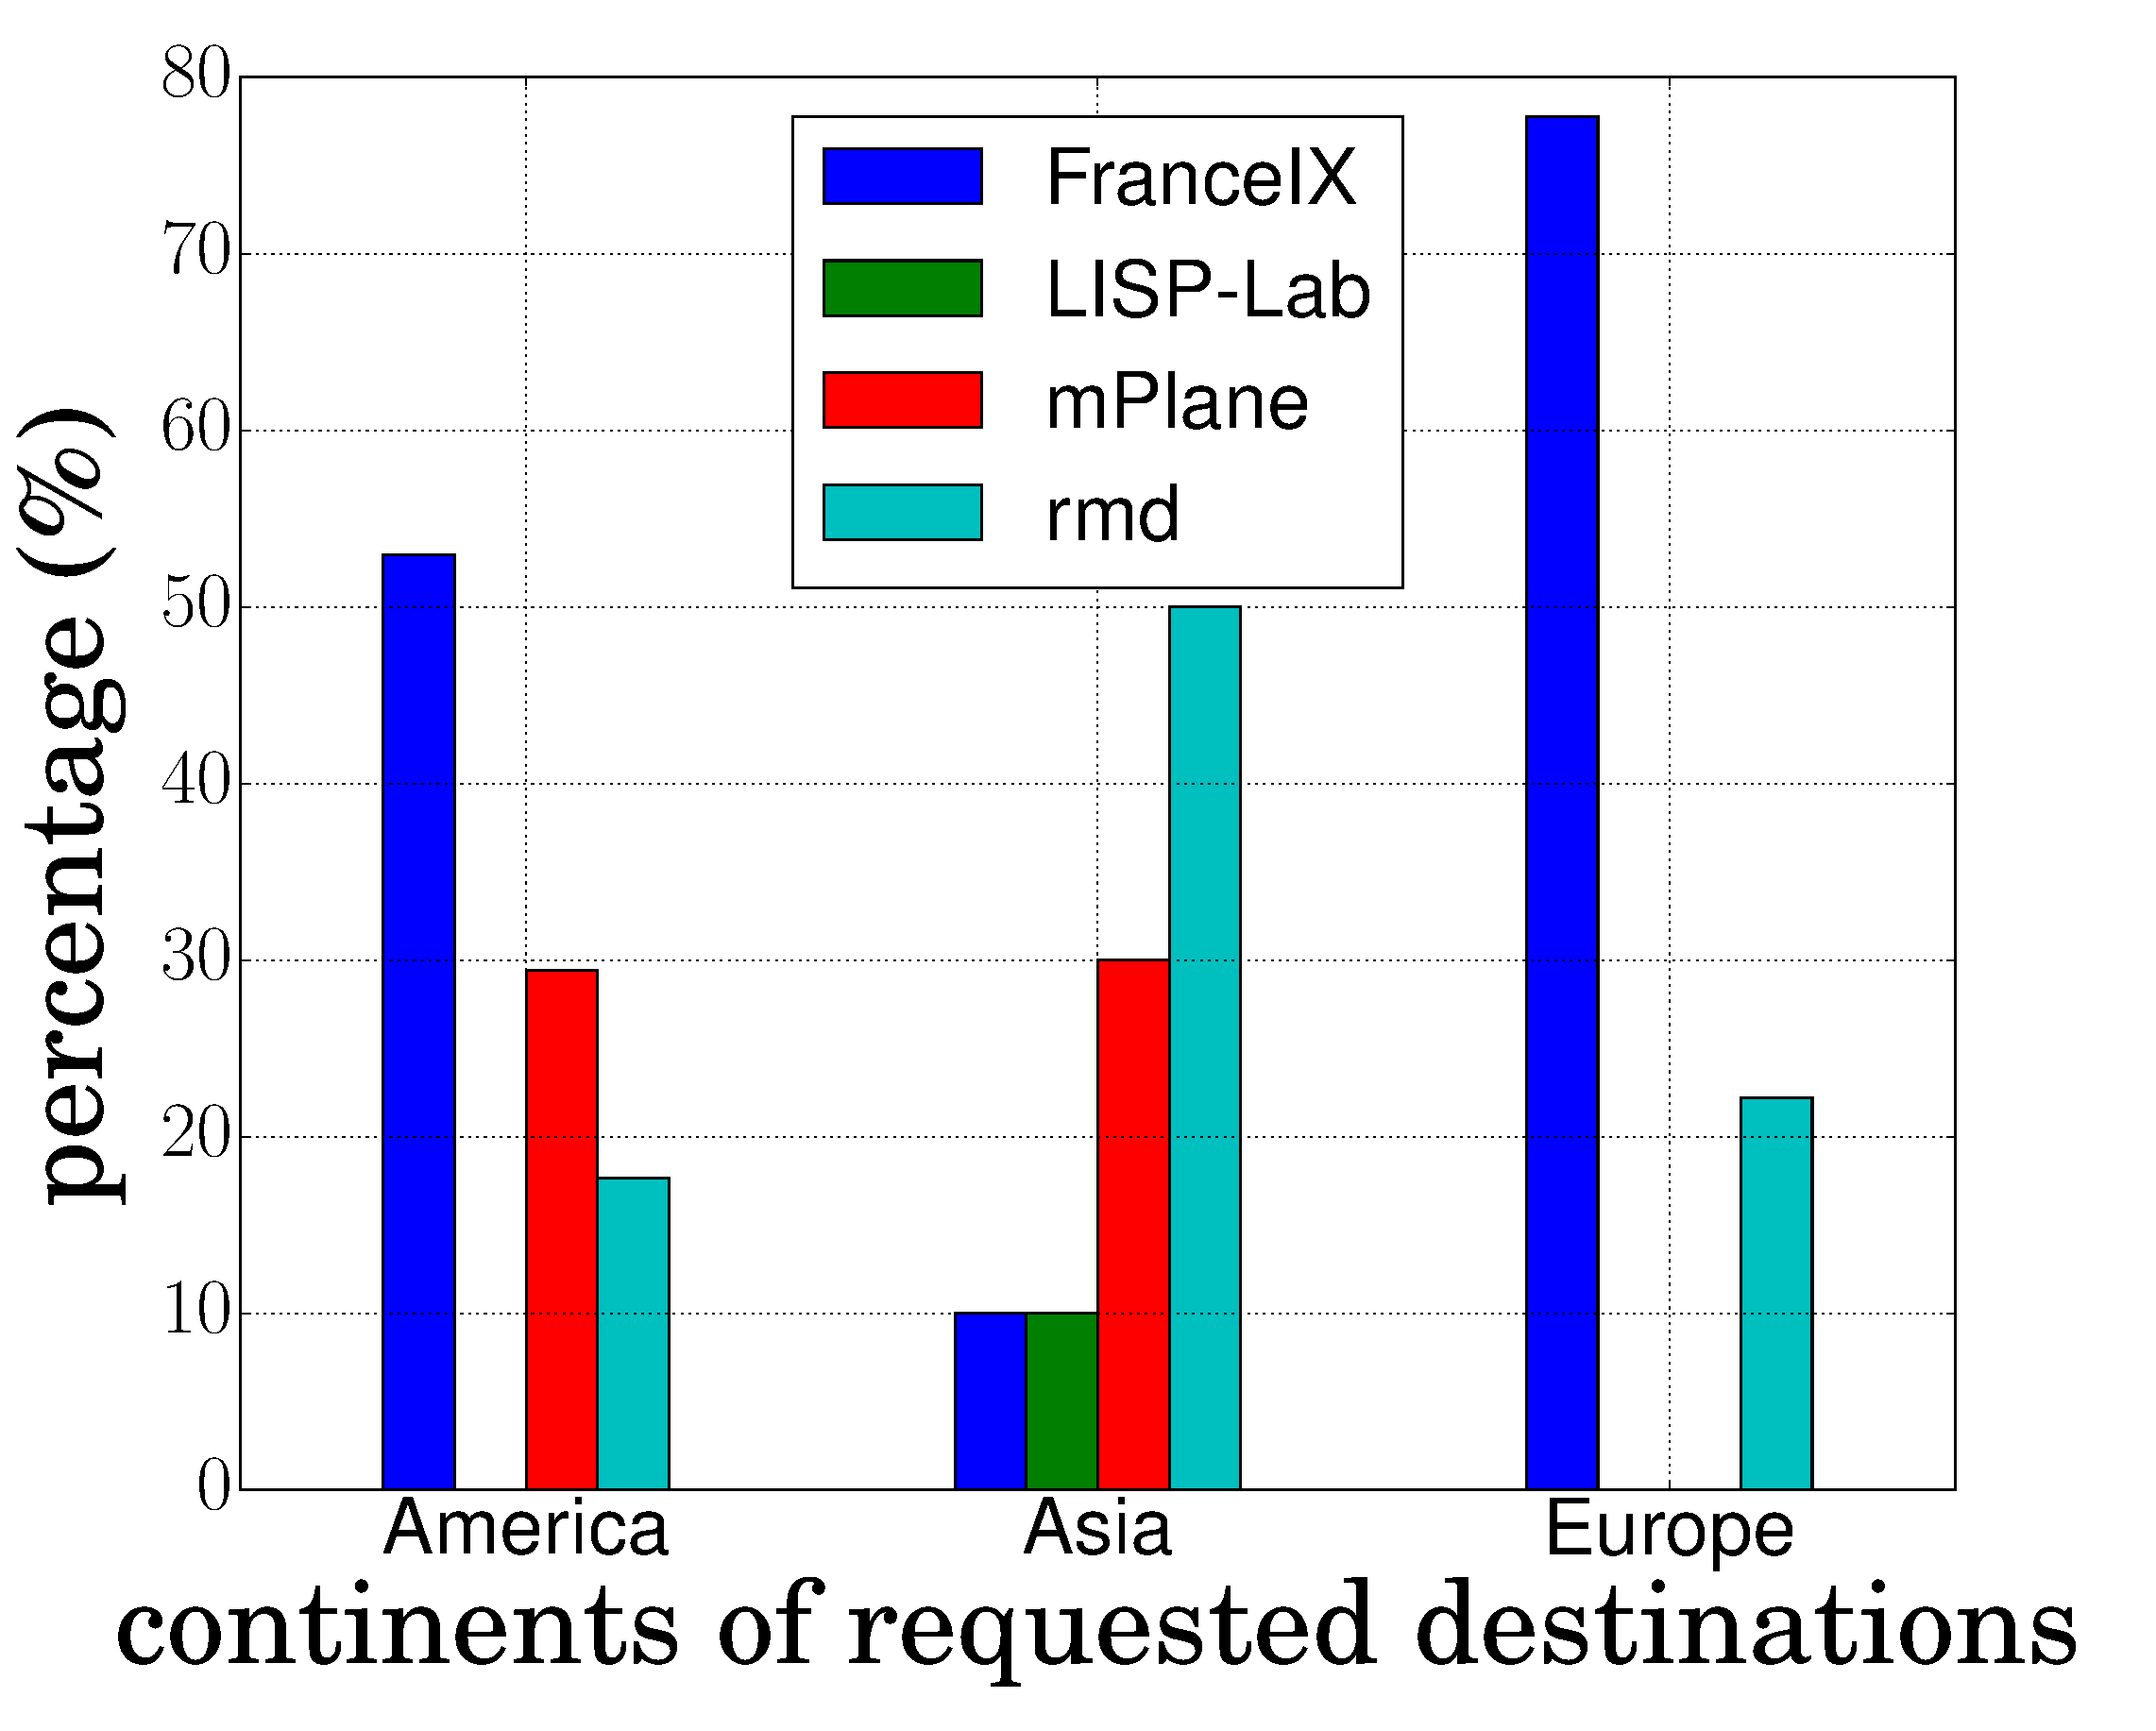
\includegraphics[width=.9\linewidth]{Pics/2015/4_probes_to_alexa_top50_proportion_median_bar_geo.eps}
		\end{center}
	\end{minipage}
	\caption{Smallest mean RTT (left) and smallest median RTT (right) grouped by continent from Dataset 2015.}
	\label{4_probes_to_alexa_top50_proportion_bar_geo}
\end{figure}
	
Fig.~\ref{4_probes_to_alexa_top50_proportion_bar_geo} depicts the percentage of times that one probe's RTT is the smallest compared to three other probes grouped by continents where the selected targets are located. When the destinations are in Europe and America, FranceIX is the fastest most of the time. % This is reasonable, since FranceIX is an Internet Exchange Point (IXP), acting as Atlas' anchor, thus it is well connected with a more powerful hardware. 
Whereas, the percentage of LISP-Lab is always 0. Its higher RTT is caused by the proxy stretch. %, since traffic between LISP-Lab probe and the legacy Internet has to pass through the LISP-Lab PxTR, which is in Lyon (approx. $400km$ away from the probe). 
When the targets are in Asia, LISP-Lab becomes the fastest with a percentage of $20\%$ (mean RTT) and $10\%$ (median RTT). It indicates that such connection from the LISP-Lab PxTR is faster, so that the stretch can be ignored. The performance of FranceIX is not very stable to the Asian destinations, being the fastest $0\%$ in average, but it is $10\%$ looking at
the median RTT. It shows that FranceIX sometimes has extremely high RTT values to Asian destinations. 
	
\begin{figure}[!t]
	\begin{minipage}[c]{.49\linewidth}
		\begin{center}
			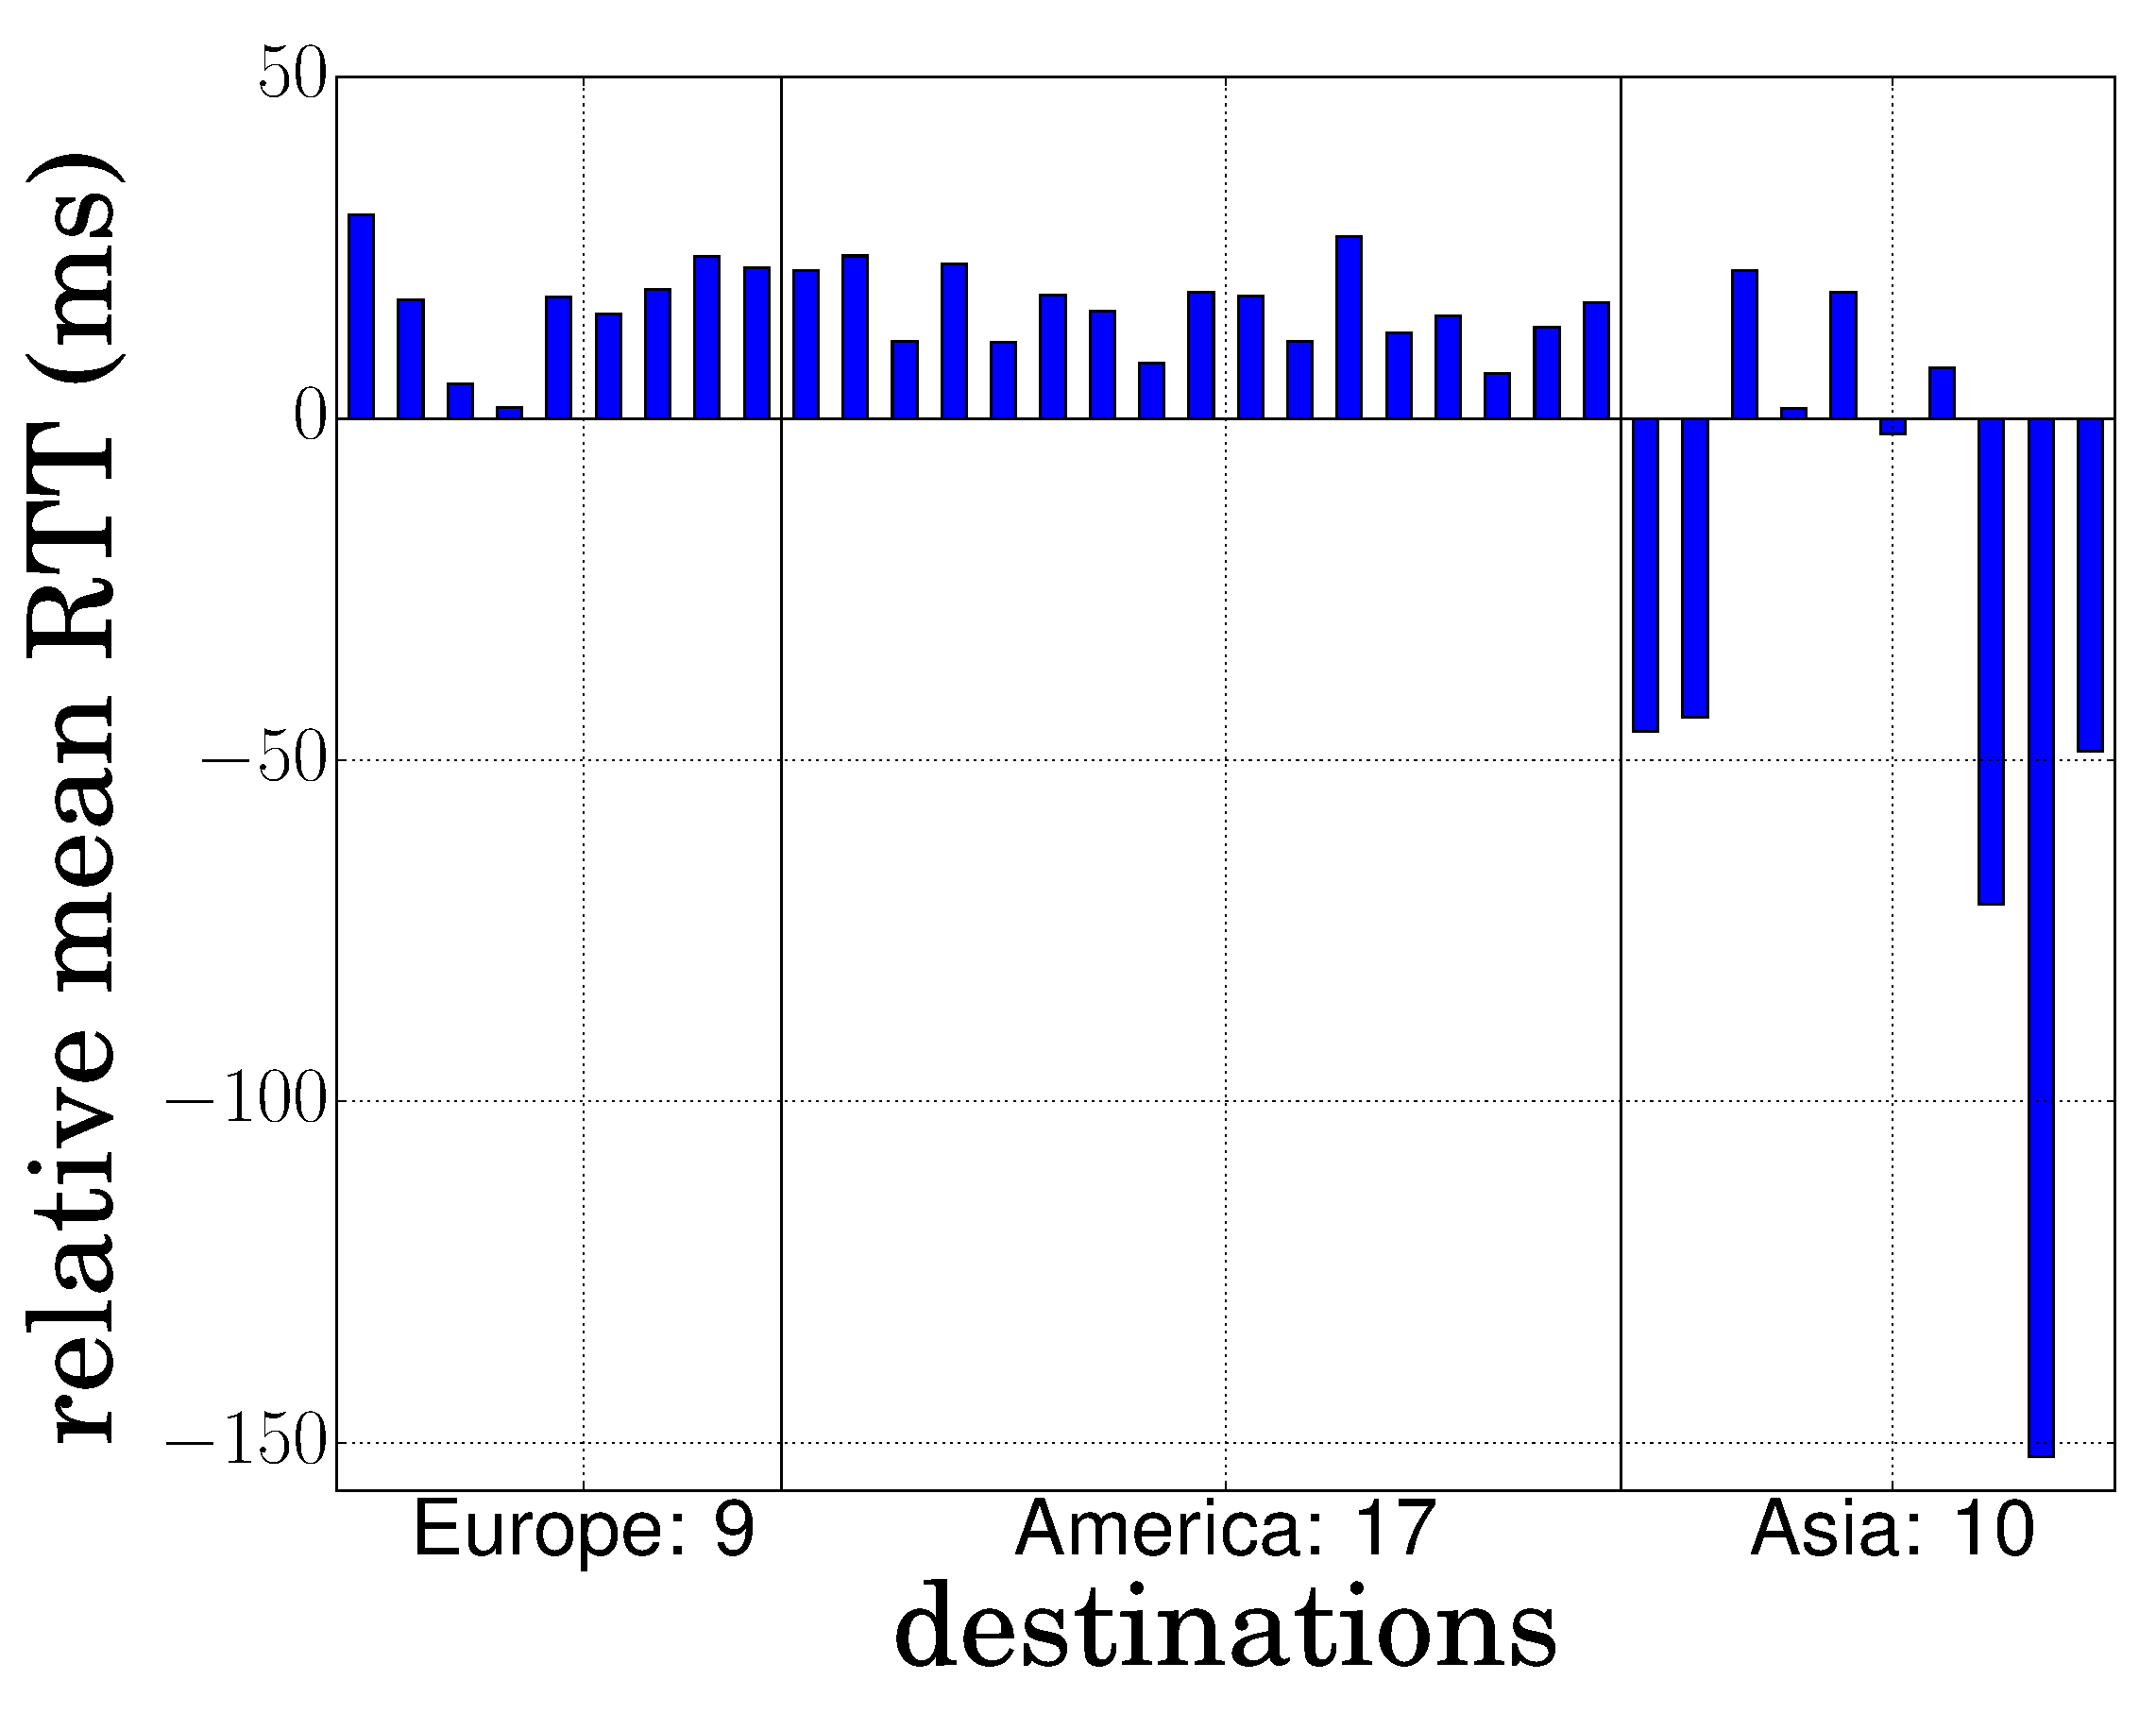
\includegraphics[width=.9\linewidth]{Pics/2015/4_probes_to_alexa_top50_diff_rtt_LISP-Lab_FranceIX_mean_geo.eps}
		\end{center}
	\end{minipage}
	\begin{minipage}[c]{.49\linewidth}
		\begin{center}
			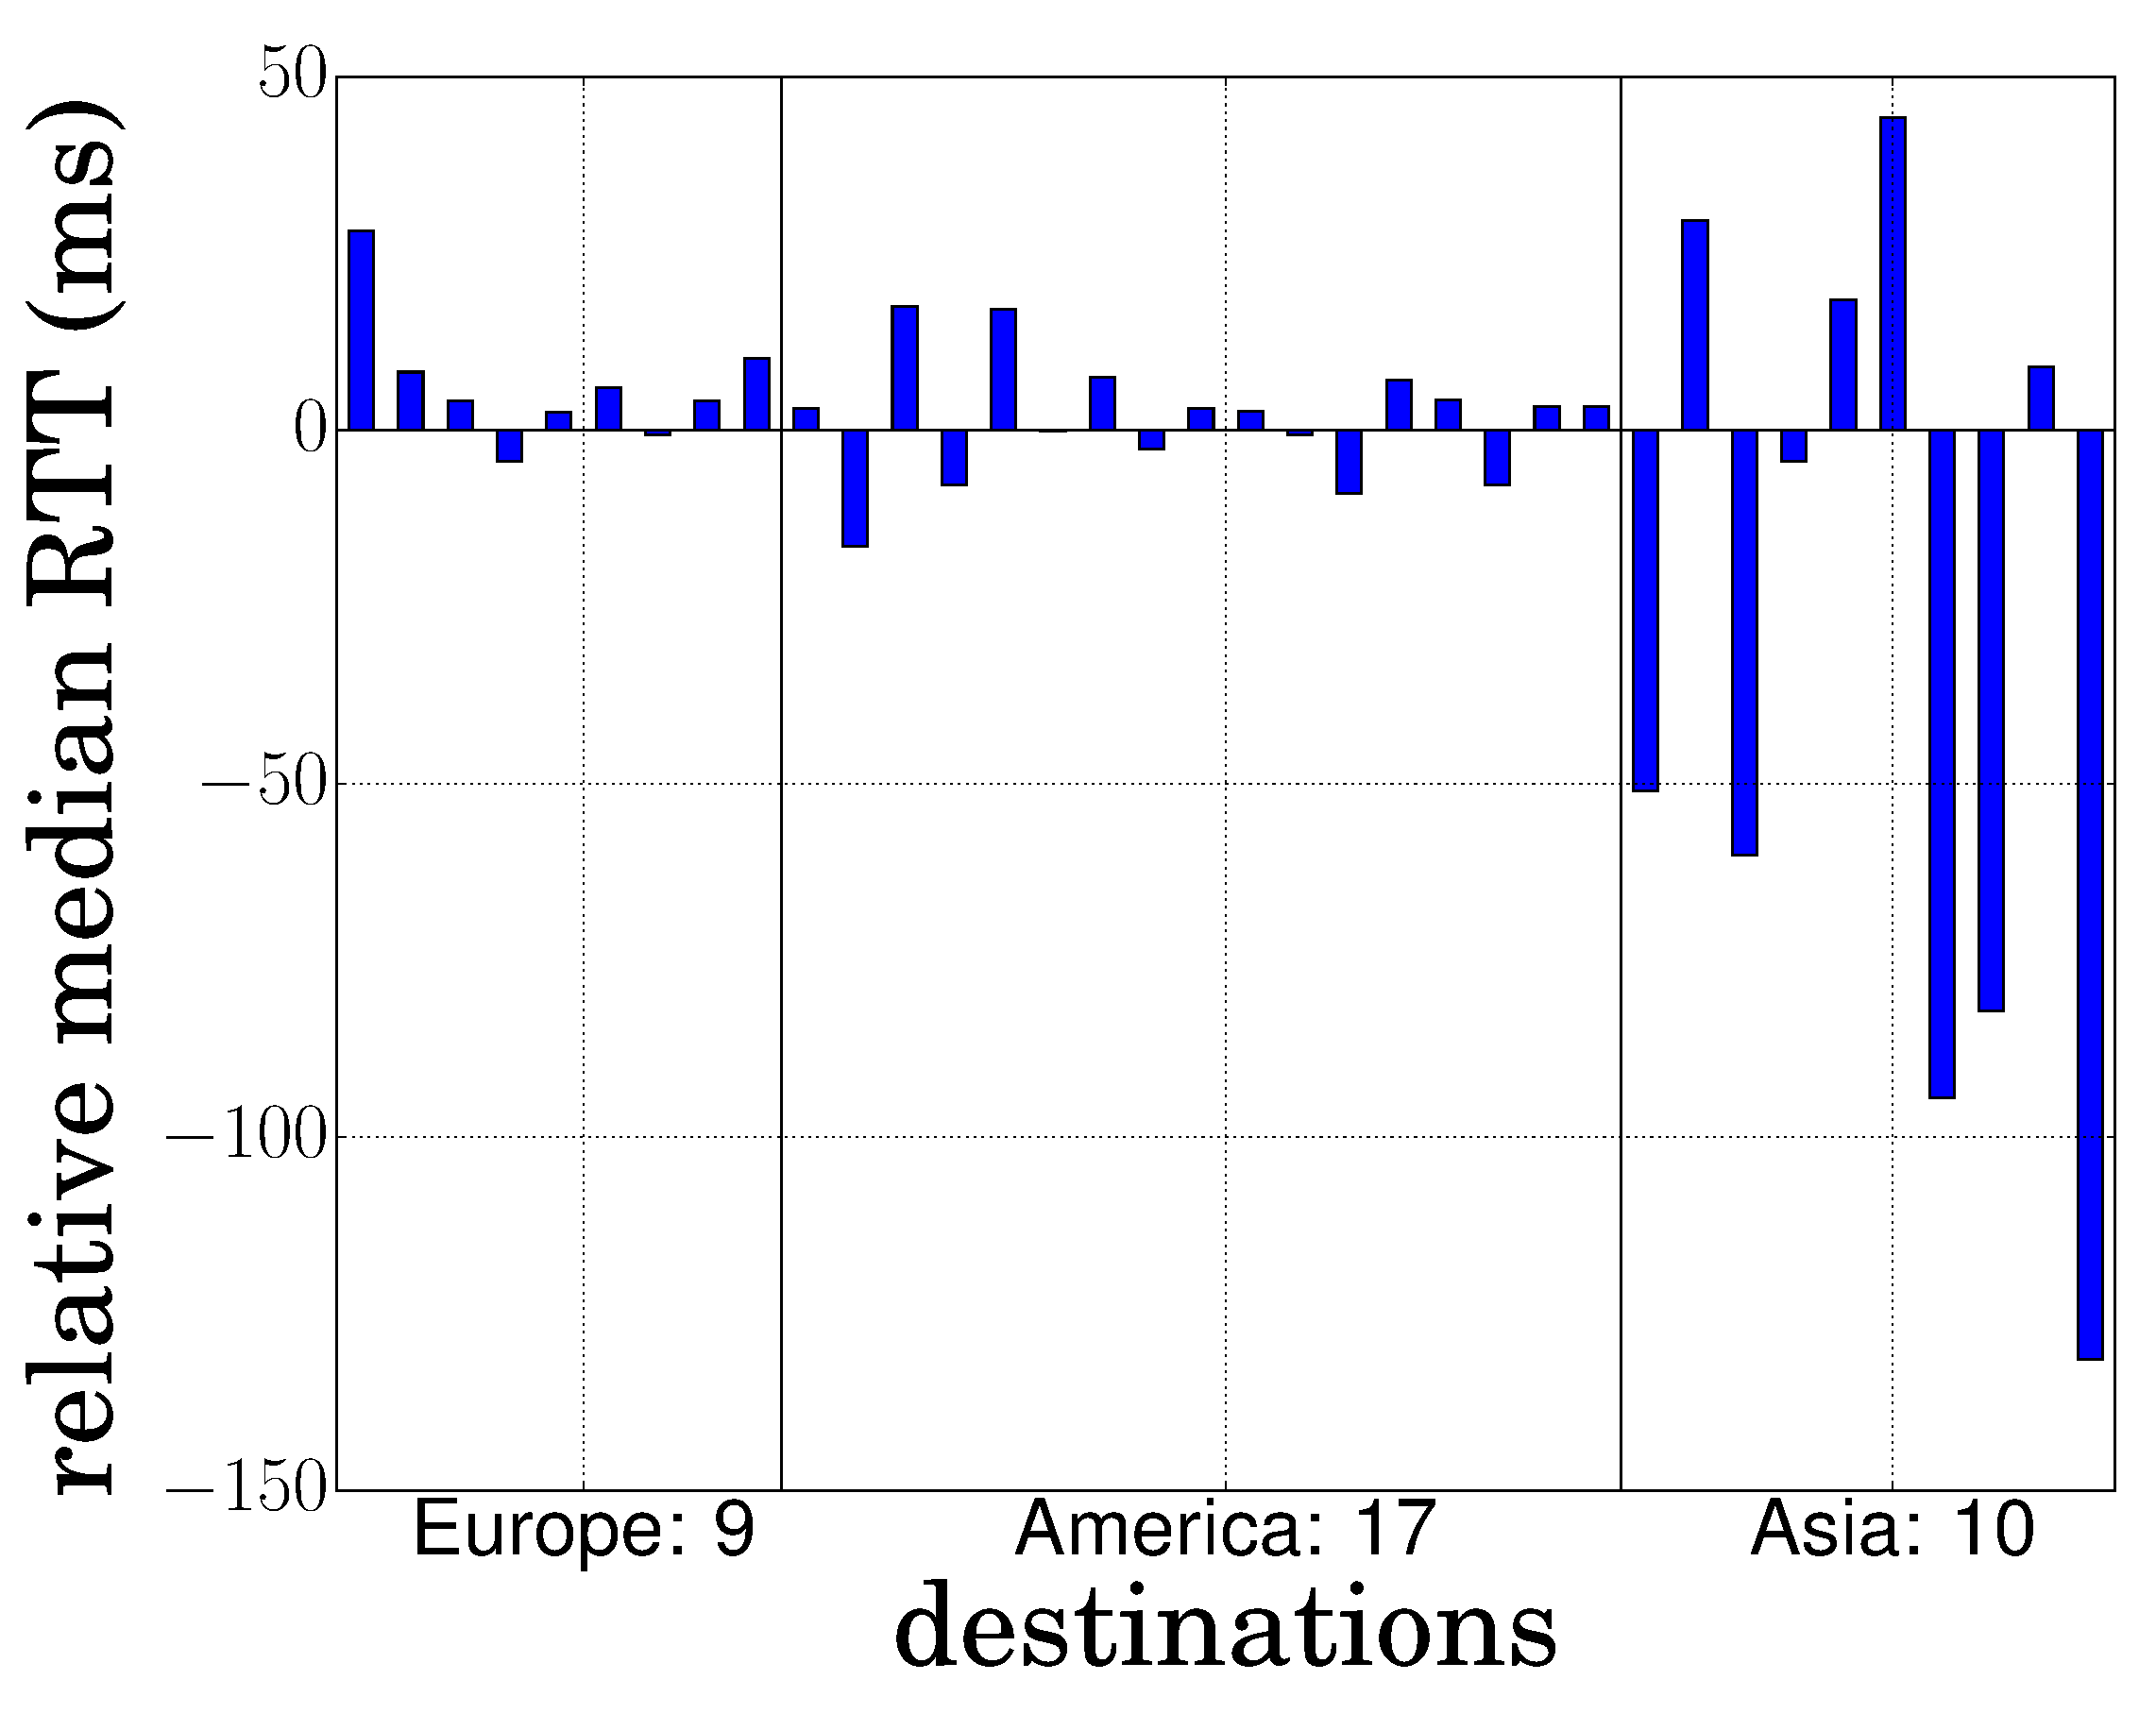
\includegraphics[width=.9\linewidth]{Pics/2015/4_probes_to_alexa_top50_diff_rtt_LISP-Lab_FranceIX_median_geo.eps}
		\end{center}
	\end{minipage}
	\vspace{-0.5mm}
	\caption{Relative mean (left) and median (right) RTT clustered by different continents from Dataset 2015.}
	\label{4_probes_to_alexa_top50_diff_rtt_LISP-Lab_FranceIX_geo}
\end{figure}
	
We also evaluate whether the performance of LISP-Lab is as stable as FranceIX. % We define the relative performance for each destination as: $RTT_{LISP-Lab}$ - $RTT_{FranceIX}$, and the results clustered by continents are shown in Fig.~\ref{4_probes_to_alexa_top50_diff_rtt_LISP-Lab_FranceIX_geo}. 
We define a metric called \emph{Relative RTT (rRTT)} for each destination as: 
\begin{equation} 
    \label{rRTT_ll_2015}
    rRTT_{LL}(d)=RTT_{LL}(d) - RTT_{F}(d)
\end{equation}
where $d$ is the destination, subscriptions $LL$ and $F$ respectively refers to LISP-Lab and FranceIX. The results clustered by continents are shown in Fig.~\ref{4_probes_to_alexa_top50_diff_rtt_LISP-Lab_FranceIX_geo}. The left hand one shows the mean RTT, while the right hand one shows the median RTT. For the European and American targets, LISP-Lab is a little slower than FranceIX but with a stable behavior. On the contrary, for half of the Asian destinations, LISP-Lab is significantly faster than FranceIX. It shows that the network connection between LISP-Lab PxTR and Asian destinations has better performance. Comparing the two subfigures, there is no negative values at all in Europe and America area in left hand figure, but there are some in the right hand one. It indicates that LISP-Lab RTTs to these destinations are very unstable and the variance is quite high.

%-< TABLE >-----------------------------------------------------------------
\begin{table}[!tb]
	\centering
	\caption{Correlation coefficient to FranceIX from Dataset 2015}
	\label{correlation_v4_2015}{
		\resizebox{0.6\textwidth}{!}{%
		\begin{tabular}{@{}c|c|c|c|c@{}}
			\hline\hline
			& LISP-Lab  & mPlane &  rmd &  FranceIX \\ \hline
			Coefficient & 0.9733  & 0.9784 &  0.9646  &  1.0     	\\  \hline\hline                 
		\end{tabular}
	}}
\end{table}
%-< END TABLE >-----------------------------------------------------------------

Since FranceIX shows the best RTT most of the time, we tried to evaluate the correlation between the RTT of the other 3 probes and FranceIX. The purpose is to see if RTT measurements are correlated or totally independent. We compute the correlation coefficient for every RTT series of different probes to all destinations with the ones of FranceIX. Tab.\ref{correlation_v4_2015} shows the results. The absolute value of coefficient is 1 in the case of a perfect direct linear relationship, whereas 0 in the case of no correlation at all. The correlation coefficient of LISP-Lab is 0.9733 (> 0.8), showing a very high correlation with FranceIX, like the other 2 probes. This means that LISP while certainly introducing some overhead, has quite stable performance that does not deviate from normal network operation.


%-< SECTION >--------------------------------------------------------------------
\section{IPv4 Ping Results from Dataset 2016}
\label{sec:pxtr_ping_v4_2016}
% \begin{itemize}[noitemsep,topsep=0pt]
%     \item CDF of median RTT between different probes
%     \item Smallest median RTT grouped by continent
%     \item Correlation coefficient to FranceIX
%     \item Relative median RTT clustered by continent for LISP-Lab and LIP6
%     \item Reliability of each probe
%     \item The periodicity check
% \end{itemize}

% With the collected dataset from IPv4 ping experiment, we assess the performance of LISP interworking with legacy Internet in terms of round-trip time (RTT).

%-< FIGURE >--------------------------------------------------------------------
\begin{figure}[!t]
	\centering
	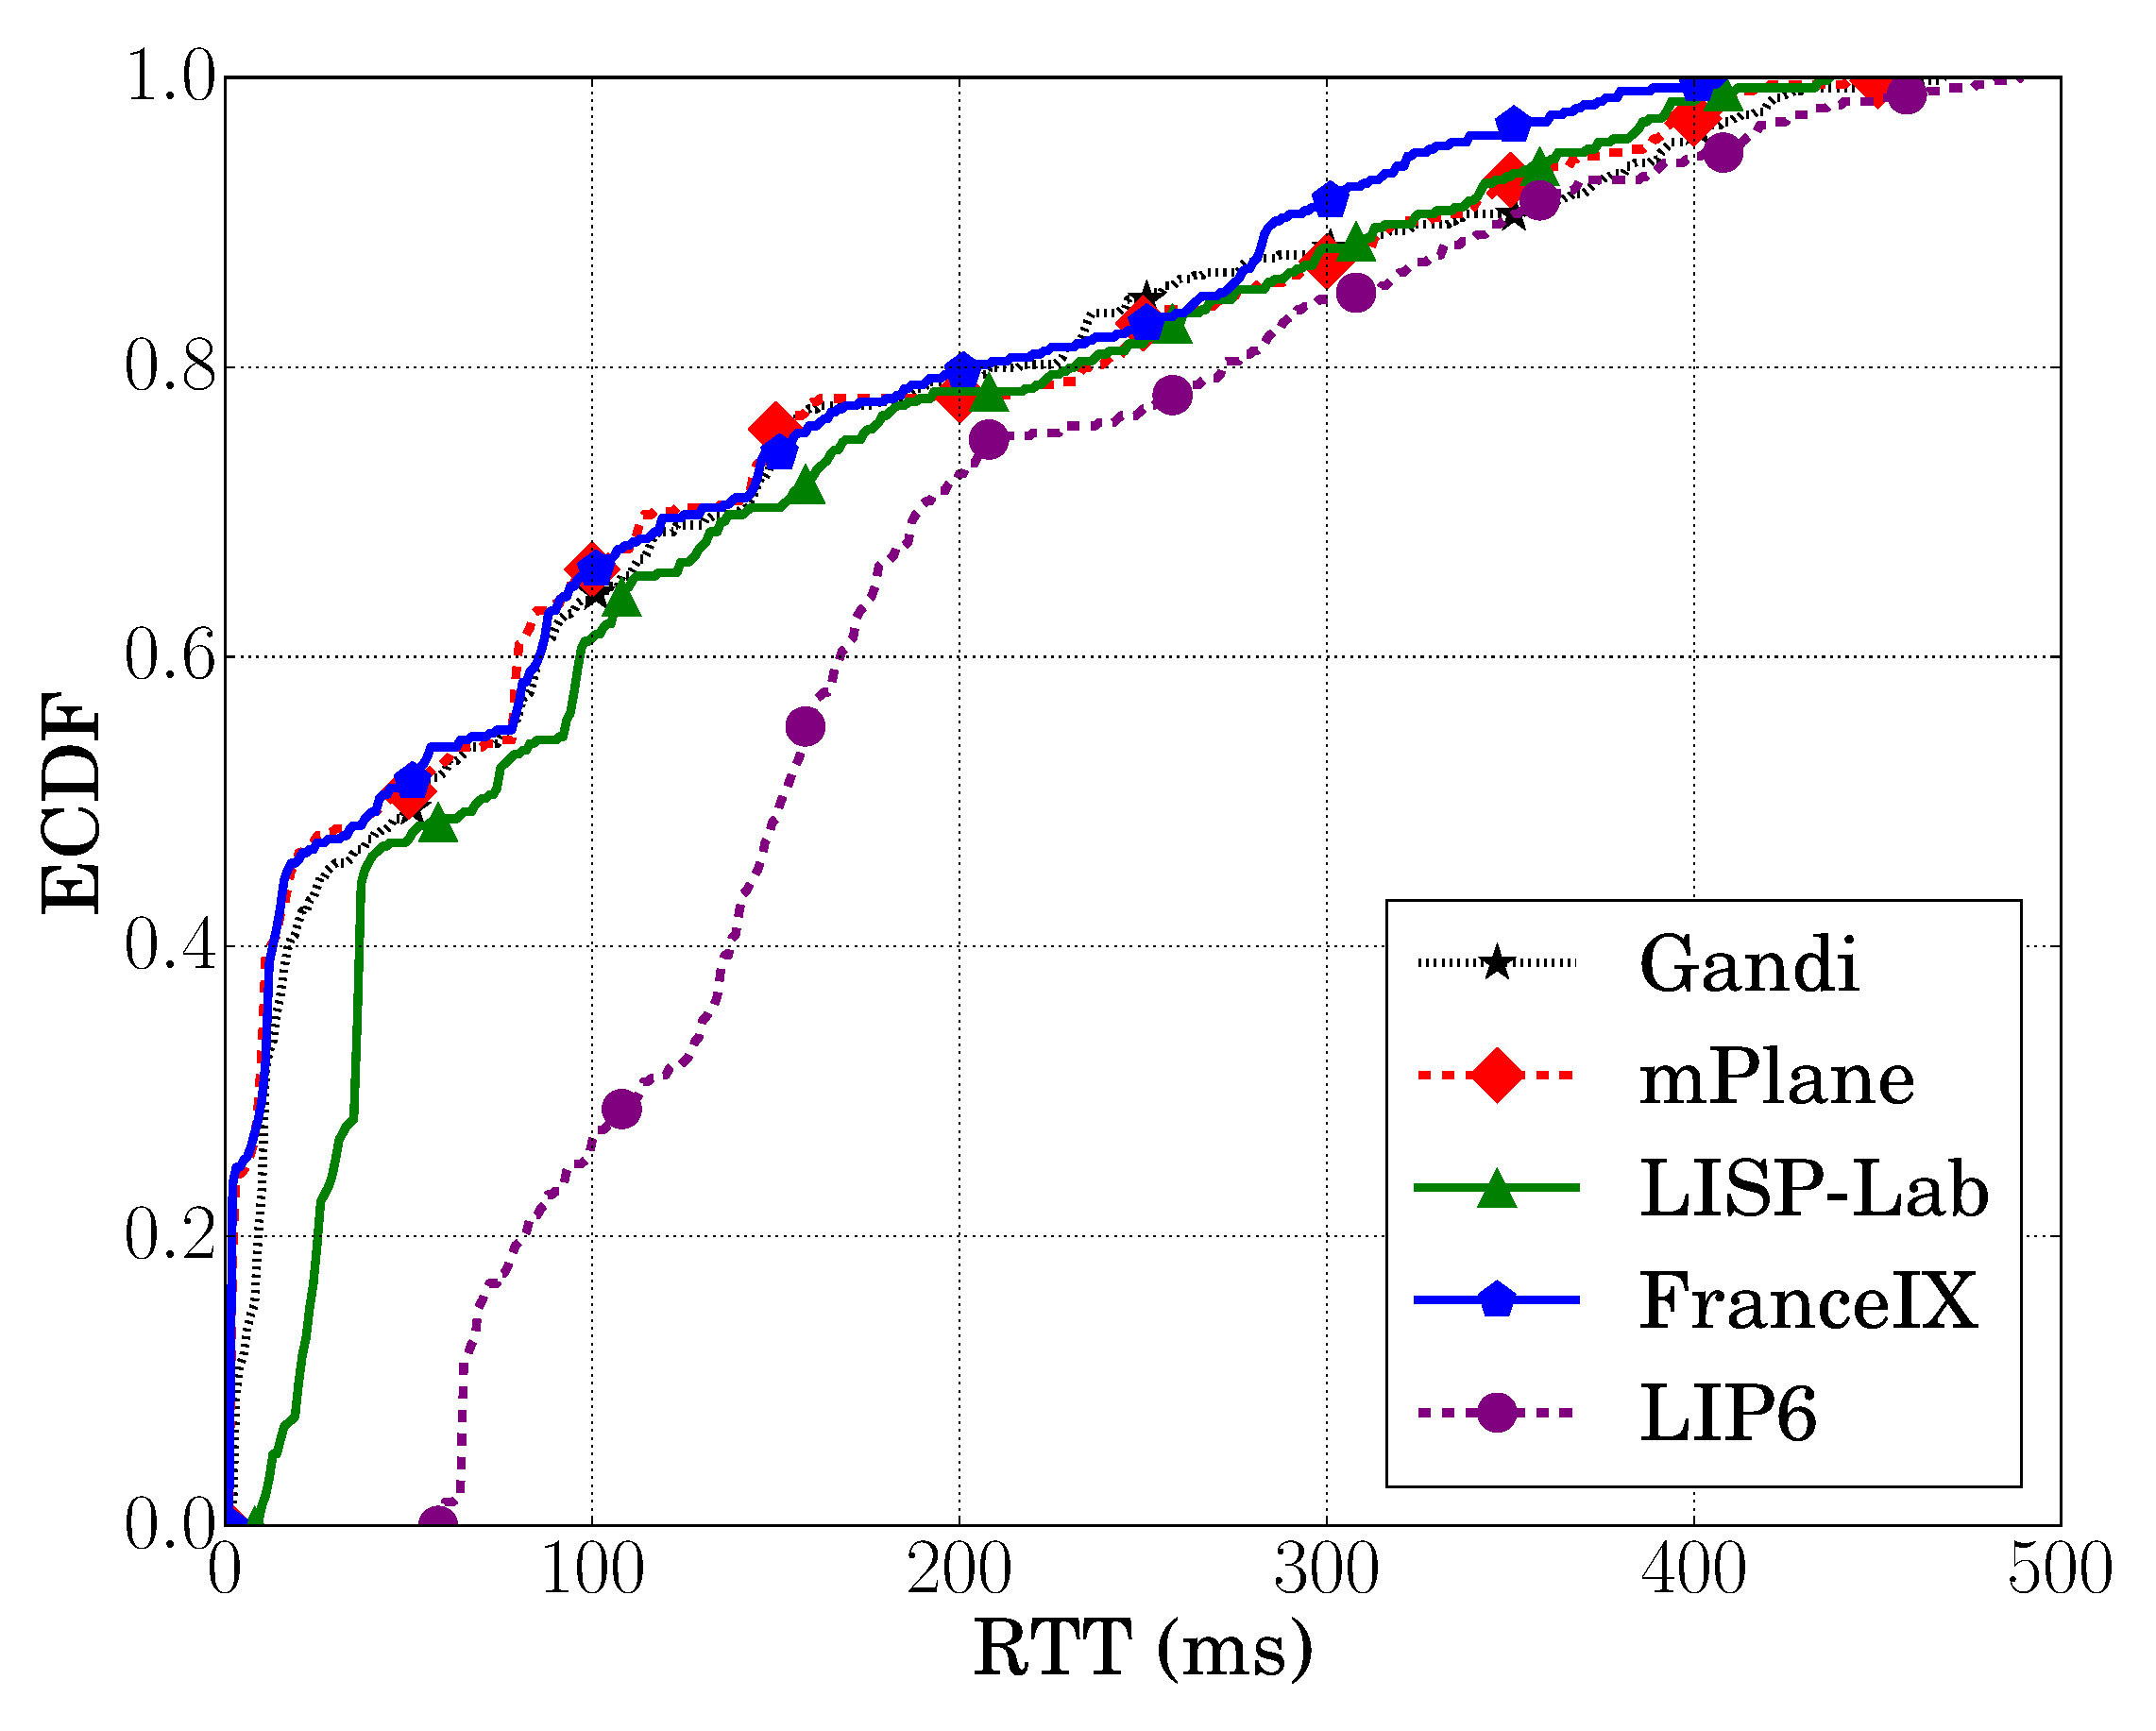
\includegraphics[width=0.6\textwidth]{Pics/v4/CDF_avg(RTT)_median_4_20.eps}
	\caption{CDF of median RTT between different probes (IPv4) from Dataset 2016}
	\label{CDF_of_median_RTT_between_different_probes_v4_2016}
\end{figure}
%-< END FIGURE >--------------------------------------------------------------------

Fig.~\ref{CDF_of_median_RTT_between_different_probes_v4_2016} shows the CDF of the average RTT toward the selected IPv4 destinations for Dataset 2016. % Because of the experimental targets are worldwide, the range of observed RTTs varies from few milliseconds (ms) to nearly 500ms. 
As an anchor, the FranceIX probe outperforms other probes in most cases, hence, showing the smallest RTT. With RTT range $[0, 200]$ms, the latency from two LISP probes, LISP-Lab and LIP6, are respectively 25ms and 60ms slower than three other non-LISP probes. Such a RTT performance degradation is caused by the path length stretch introduced by the the proxy technology (as mentioned in Sec.~\ref{sec:background_lisp}), since every packet sent between LISP probe and the legacy Internet has to pass through a PxTR. Although both LISP probes introduce the stretch, LIP6 probe is even 50ms slower than the LISP-Lab probe. Given that both LISP-Lab and LIP6 probes pass through the same PETR located in Lyon, the performance degradation of LIP6 probe is due to the PITR selection for traffic from legacy Internet to LISP network. The PITRs used by LIP6 probe belongs to the LISP Beta Network and there are in total 6 available PITRs. The PITRs announce the LISP Beta prefixes to their AS peers using BGP. So different destinations select different PITRs depending on where the destinations are and lead to the reply goes through the different paths. For example, an Asian destination normally uses the PITR in Japan instead of selecting one in Europe. As listed in Tab.~\ref{PxTR_loc_2016}, LISP Beta Network has not deployed PITR in France, while the PITR of LISP-Lab is in the same country to its probe. Thus, the return path that we measured for the LIP6 probe is longer than for the LISP-Lab probe. As a result, the closer the destination is located to the probes, the bigger the difference of RTT between the two LISP probes.

Within RTT range $[200, 500]$ms, all probes except LIP6 show basically the same RTT. It indicates that LISP-Lab has a better performance in scenario of long distance network connection. The reason is that stretch delay from LISP-Lab probe to PxTR (in Lyon) can be ignored. Fig.~\ref{CDF_of_median_RTT_between_different_probes_v4_2016} confirms this situation, within RTT range $[200, 500]$ ms, the difference between two probes becomes significantly smaller than that in range $[0, 200]$ ms.

The aforementioned results and analysis coincide with the Fig.~\ref{CDF_RTT_avg_v4_2015} from the dataset of 2015, which just covers comparison related to LISP-Lab probe. This indicates that the LISP PxTR performance is stable: the measurement results do not change with the different destinations at the different time. 

%-< FIGURE >--------------------------------------------------------------------
\begin{figure}[!t]
	\centering
	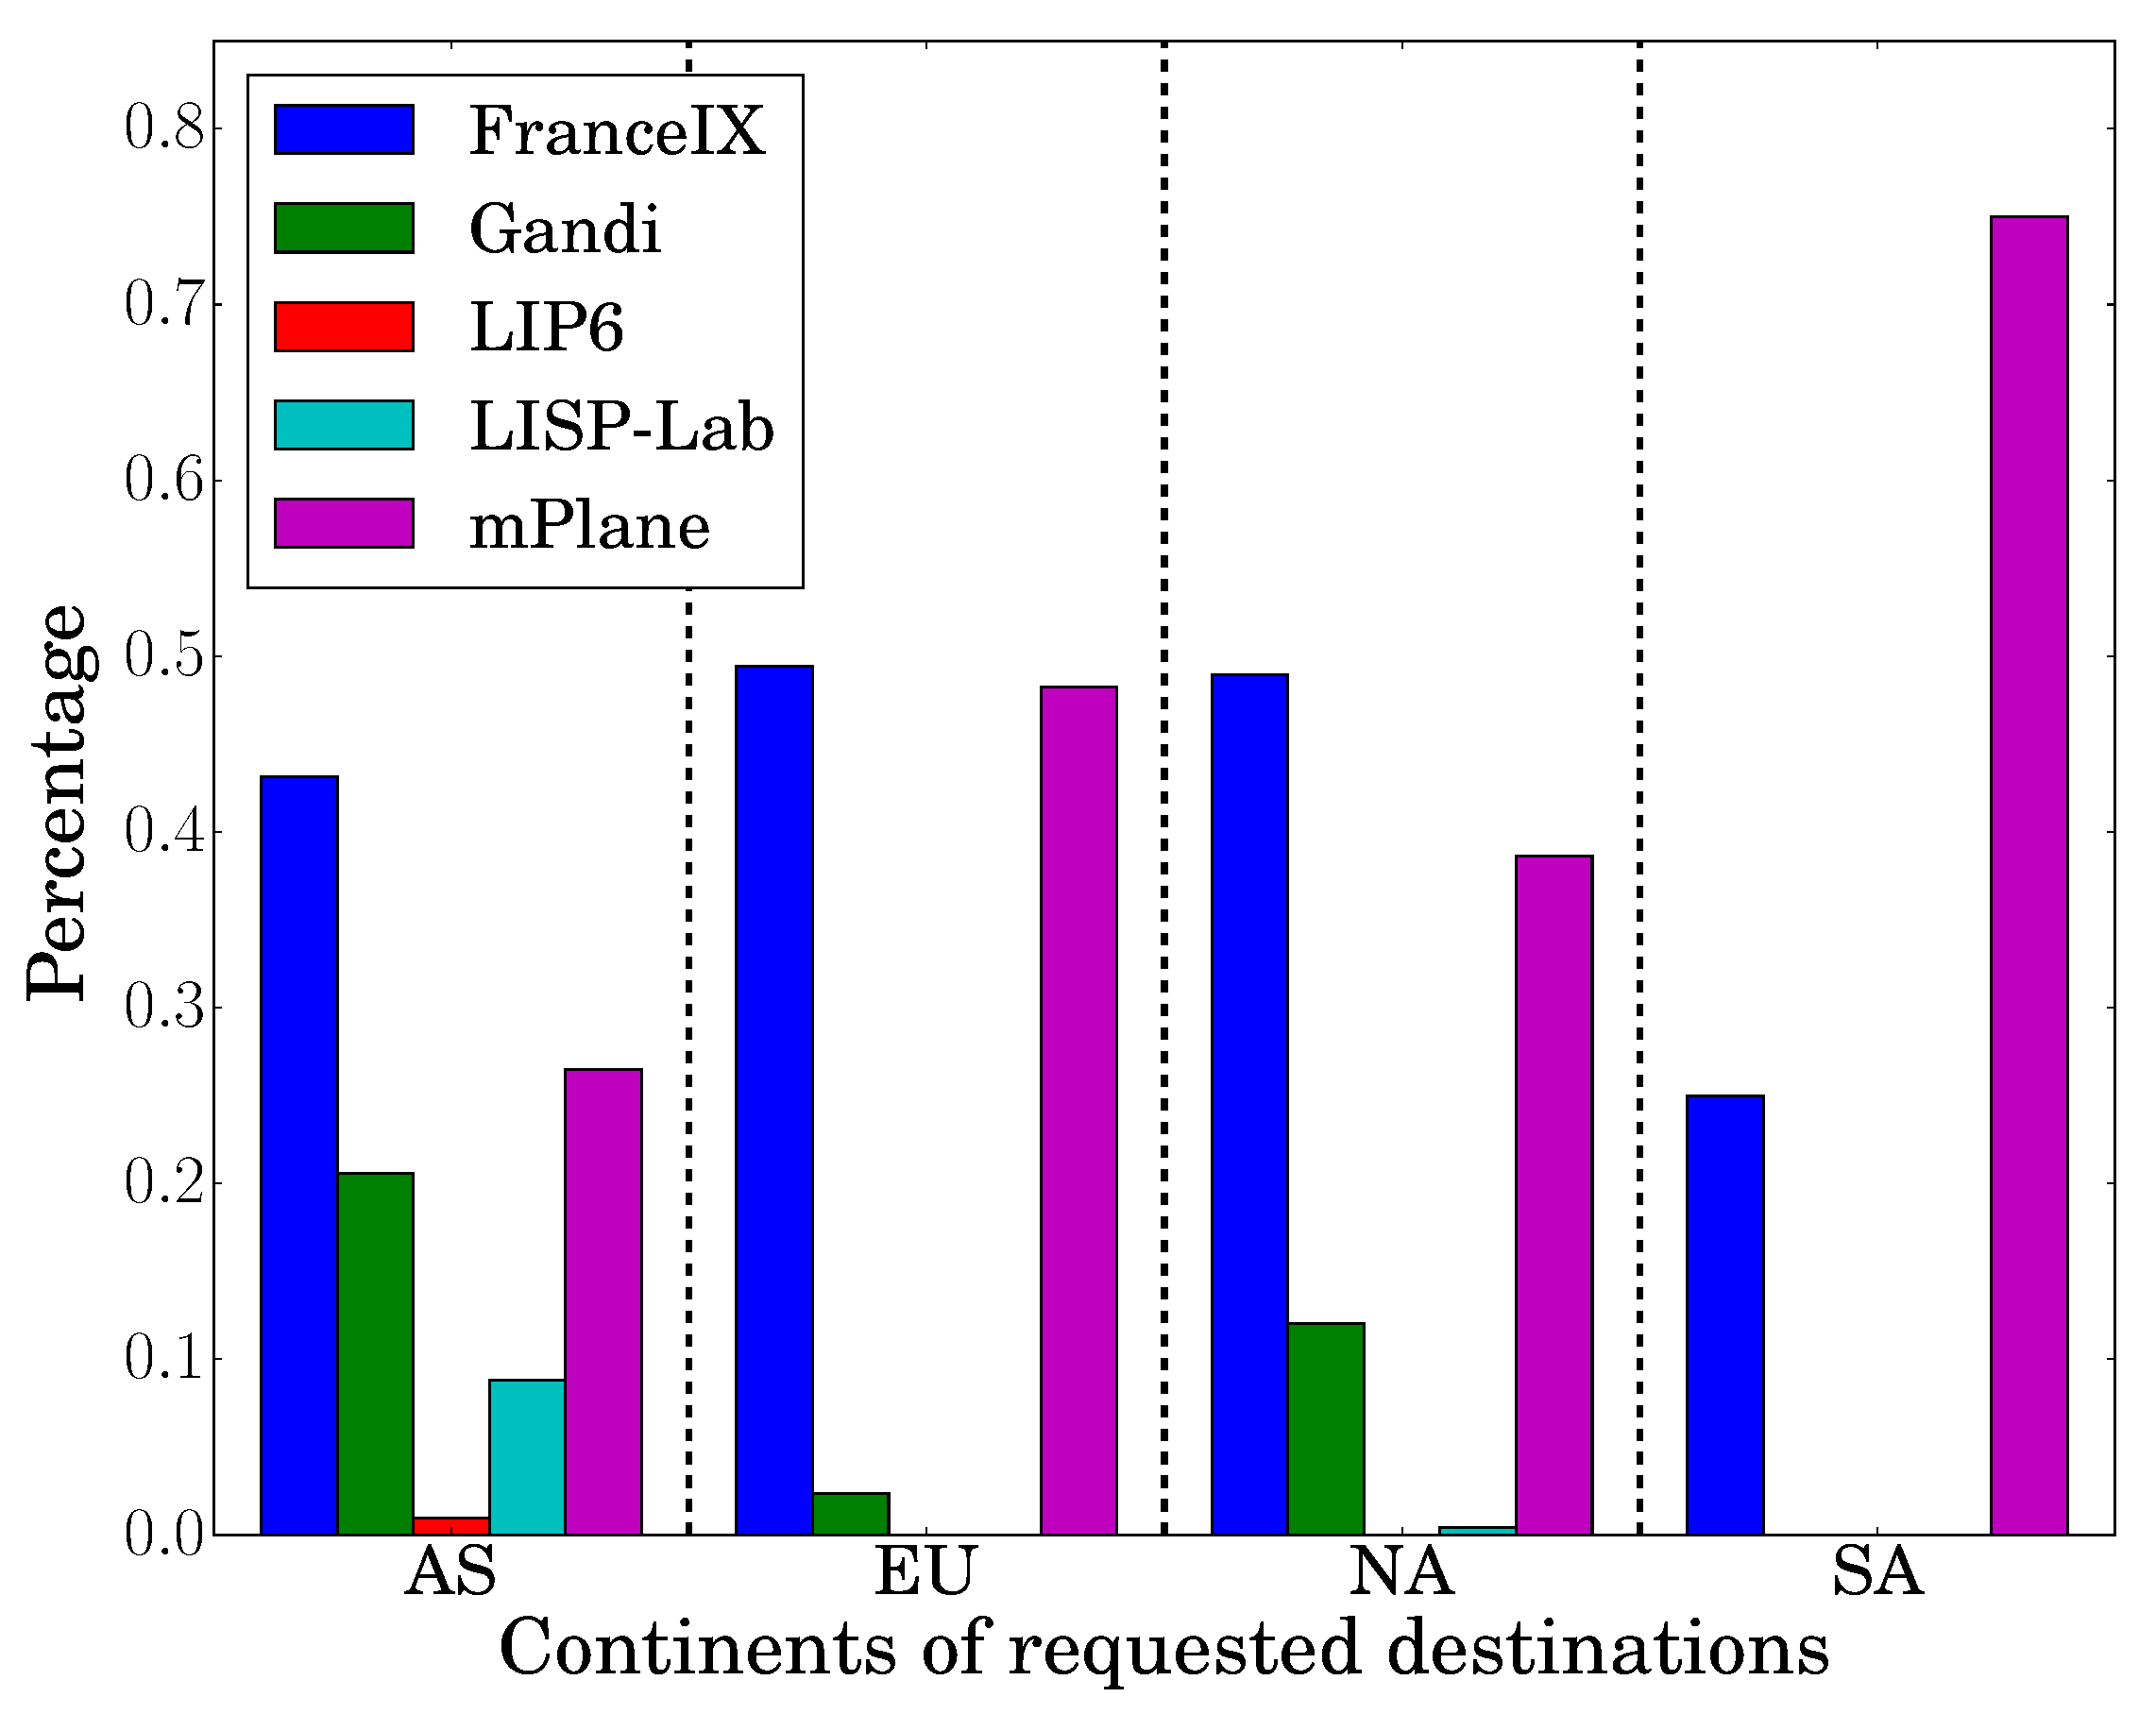
\includegraphics[width=0.6\textwidth]{Pics/v4/Smallest_median_avg(RTT)_proporation.eps}
	\caption{Smallest median RTT grouped by continent (IPv4) from Dataset 2016.}
	\label{Smallest_median_avg(RTT)_proporation_v4_2016}
\end{figure}
%-< END FIGURE >--------------------------------------------------------------------

Even with stretch brought by the PxTR, LISP probes still outperform non-LISP probes in some cases according to the measurement results. To identify these cases, worldwide destinations are classified by continent.
Fig.~\ref{Smallest_median_avg(RTT)_proporation_v4_2016} depicts the percentage of times that one probe has the smallest RTT compared to the other probes grouped by continents where the selected targets are located.
The experimental destinations are located in 4 continents, i.e., Europe, North America, South America, and Asia. The \emph{ping} measurement is repeated 720 times as the experiment lasts 15 days and its interval is 30 minutes. The RTTs of the FranceIX anchor and mPlane probe are the smallest most of the time, especially for the European and South American destinations. Only for the Asian destinations the RTT of LISP-Lab probe experiences sometimes the smallest latency for $8.82\%$ of the targets, while the LIP6 probe experiences the smallest latency in $0.98\%$ of the cases. Among the North American destinations, there is just one destination for which the RTT of the LISP-Lab probe is the smallest, while there is no destination for which LIP6 experiences the smallest latency. Fig.~\ref{CDF_of_median_RTT_between_different_probes_v4_2016} shows that for RTT above $200ms$ LISP-Lab performs like the other probes, so that we can question whether it actually has the best performance in some cases, and for which destinations. Fig.~\ref{Smallest_median_avg(RTT)_proporation_v4_2016} shows the geographic location of destinations for which LISP-Lab actually is the best performing probe. In particular, the LISP-Lab probe has no additional delay compared to other non-LISP probes for the intercontinental transmission to the Asian destinations. It means that the negative effect of LISP stretch delay is evident for communications with European and American destinations, but can be neglected for Asian intercontinental destinations. This phenomenon is similar to the result shown in~\cite{li2016performance}, which shows only in $5.6\%$ of the cases that the LISP-Lab probe experiences the smallest latency and all these destinations are in Asia. It proves again that the negative effect of LISP PxTR can be ignored for the intercontinental transmission to the Asian destinations (when considering the European vantage point).

 %-< TABLE >-----------------------------------------------------------------
 %%%%%%%%%%%%%%% Table %%%%%%%%%%%%%%% 
 \begin{table}[!tb]
 	\centering
 	\caption{Correlation coefficient to FranceIX (IPv4) from Dataset 2016}
 	\label{correlation_v4_2016}{
 	\resizebox{0.7\textwidth}{!}{%
 		\begin{tabular}{@{}c|c|c|c|c|c@{}}
 			\hline\hline
 			 & Gandi  & mPlane  & LISP-Lab  & LIP6 &  FranceIX \\ \hline
 			Coefficient &  0.9647 & 0.9707 & 0.9766 & 0.8547 & 1.0     	\\  \hline\hline                 
 		\end{tabular}
 	}}
 \end{table}
 %-< END TABLE >-----------------------------------------------------------------

% As FranceIX is an enhanced probe with more measurement capacities presenting more stable performance, 
Also for the Dataset 2016, we try to evaluate the correlation in term of RTT between FranceIX and other probes. % The purpose is to see if RTT measurements are correlated or totally independent. The method is to compute the correlation coefficient for every RTT series of different probes to all destinations with the ones of FranceIX. The results are shown in Tab.~\ref{correlation_v4_2016}. The absolute value of coefficient is 1 in the case of a perfect direct linear relationship, whereas 0 in the case of no correlation at all, i.e., independent. 
The correlation coefficient of LISP-Lab is 0.9766 (> 0.8), showing a very high correlation level with FranceIX, and even higher than the correlation coefficient of all the other probes. The correlation coefficient of LIP6 is 0.8547, shows a high correlation with FranceIX as well. Both LISP probes having a high correlation with FranceIX means that while certainly introducing some overheads, LISP has quite stable performance that does not deviate from normal network operation. Such result has two sides for the performance of LISP. Good because LISP shows stability. Bad because it means that LISP experiences the same performance and failures like the normal Internet.

%-< FIGURE >--------------------------------------------------------------------
\begin{figure}[!t]
	\begin{minipage}[c]{.49\linewidth}
		\begin{center}
			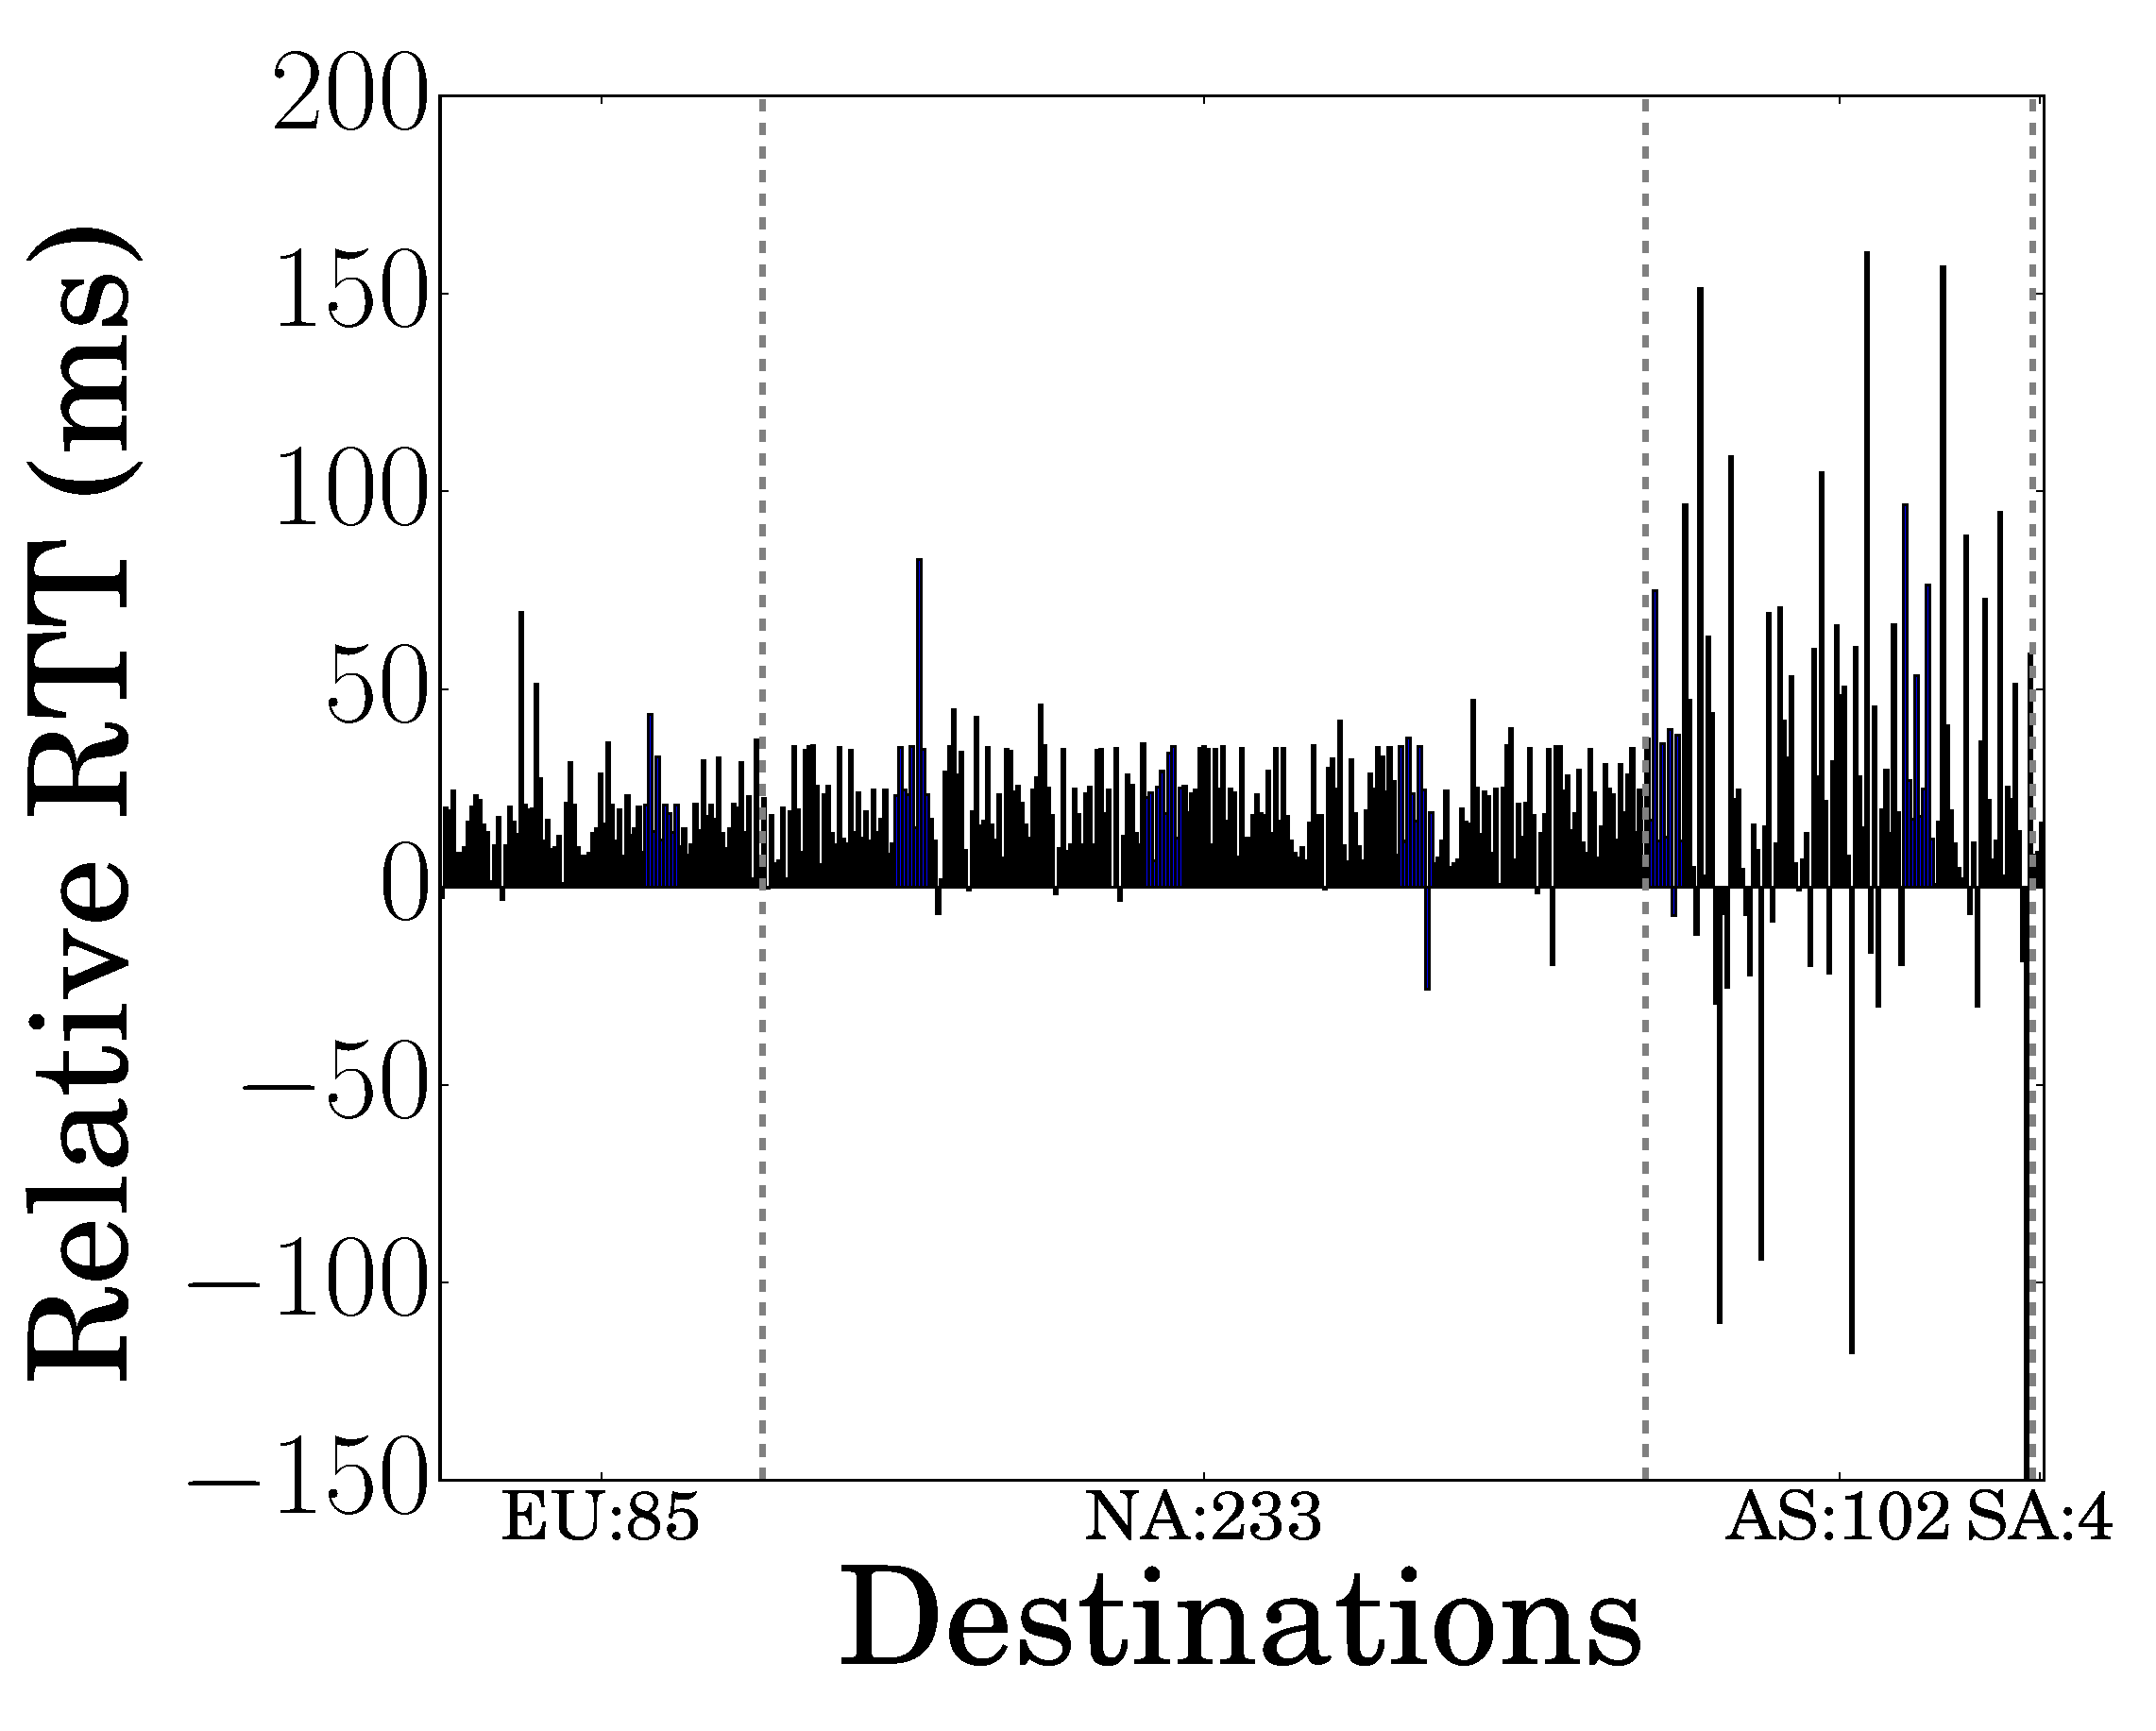
\includegraphics[width=\textwidth]{Pics/v4/Relative_median_avg(RTT)_LISP-Lab-FranceIX_changed_60.eps}
		\end{center}
	\end{minipage}
	\begin{minipage}[c]{.49\linewidth}
		\begin{center}
			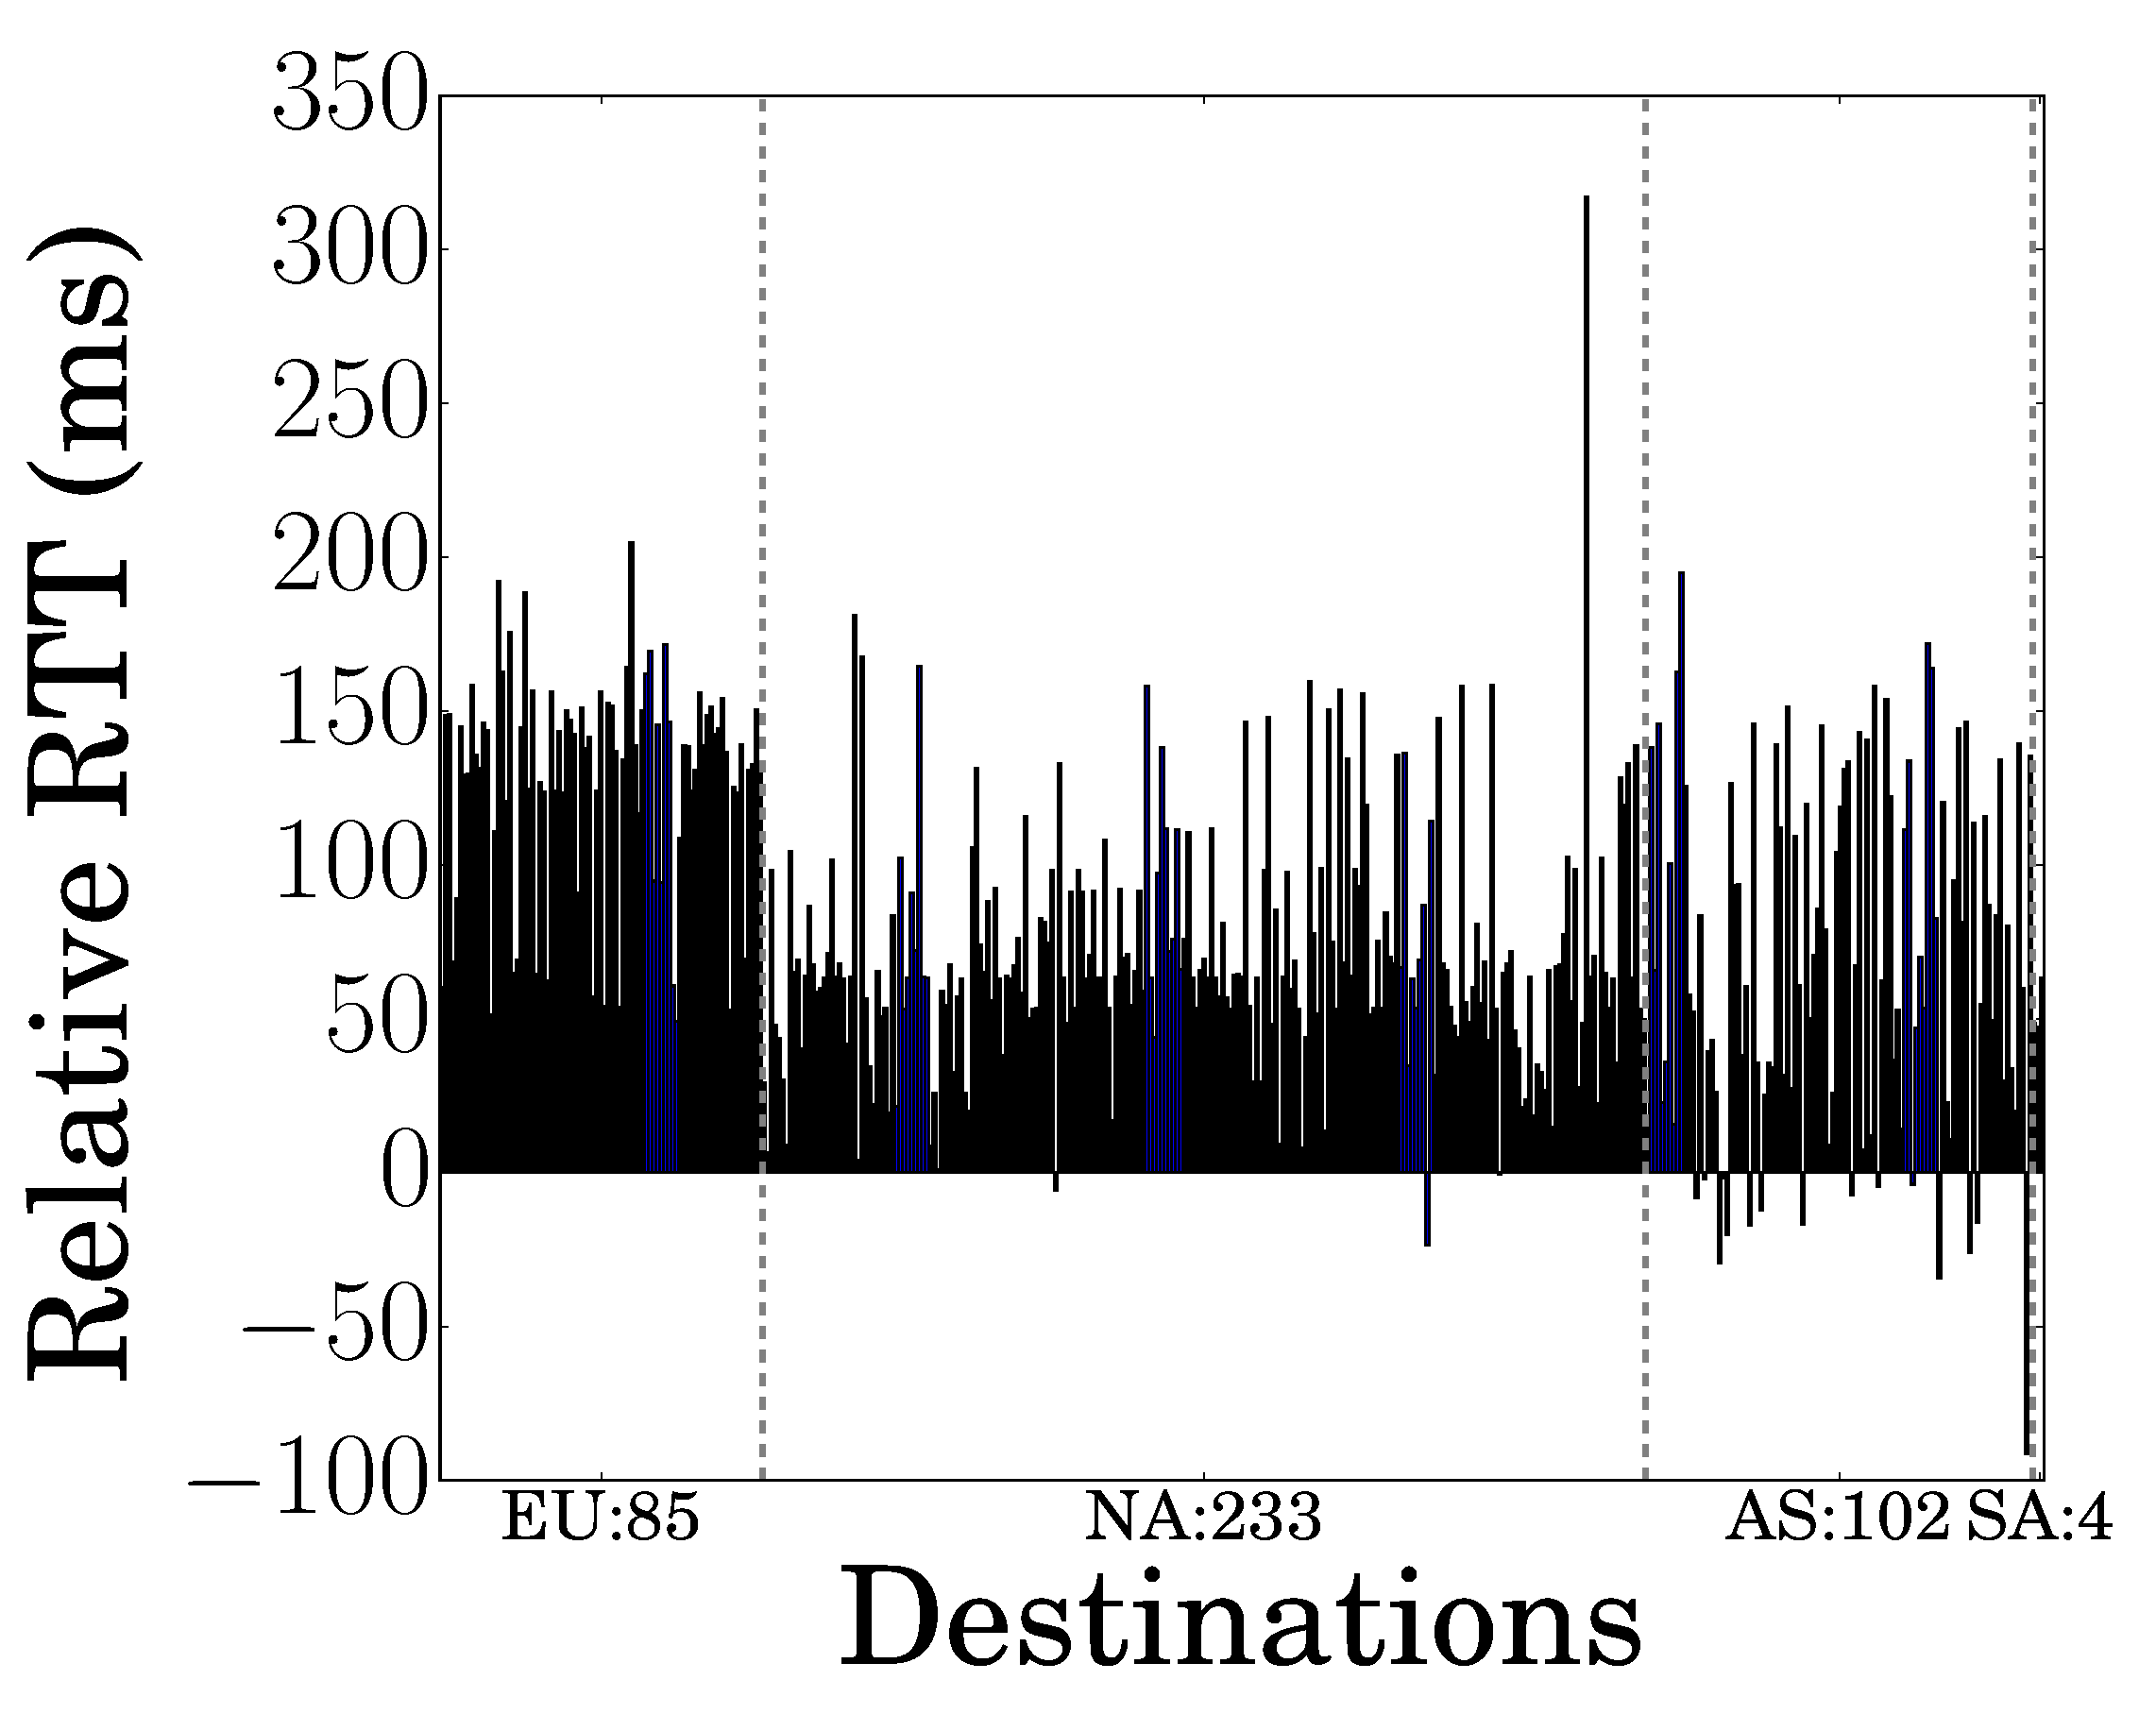
\includegraphics[width=\textwidth]{Pics/v4/Relative_median_avg(RTT)_LIP6-FranceIX_changed_60.eps}
		\end{center}
	\end{minipage}
	\vspace{-0.5mm}
	\caption{IPv4 Relative median RTT clustered by different continents for LISP-Lab (left) and LIP6 (right) from Dataset 2016}
	\label{Relative_median_avg(RTT)_v4_2016}
\end{figure}
%-< END FIGURE >--------------------------------------------------------------------
Another interesting point is to asses whether the two LISP probes have a stable performance as FranceIX according to the destinations. To this end, we leverage on the same metric of \emph{Relative RTT (rRTT)} (formula~\ref{rRTT_ll_2015}), defined in Sec.~\ref{sec:pxtr_ping_v4_2015} for each destination as: 
\begin{equation} 
    \label{rRTT_ll_2016}
    rRTT_{LL}(d)=RTT_{LL}(d) - RTT_{F}(d)
\end{equation}
\begin{equation}
    \label{rRTT_l6_2016}
    rRTT_{L6}(d) = RTT_{L6}(d) - RTT_{F}(d)
\end{equation}
where $d$ is the destination, subscriptions $LL$, $L6$ and $F$ respectively refers to LISP-Lab, LIP6 and FranceIX. The results clustered by continents are shown in Fig.~\ref{Relative_median_avg(RTT)_v4_2016}, where the relative RTT for LISP-Lab probe is on the left and the relative RTT for LIP6 probe is on the right. The positive relative RTT indicates FranceIX faster, while the negative values indicating that LISP-Lab or LIP6 are faster. In the left side of Fig.~\ref{Relative_median_avg(RTT)_v4_2016}, for the European and American targets, the values are between 10ms and 20ms in most cases (i.e., 31.37\%), showing that LISP-Lab is a little slower than FranceIX but with a stable behavior. On the contrary, for some Asian destinations, LISP-Lab is significantly either faster (in $20.6\%$ of the cases) or slower than FranceIX and the largest difference reaches 150ms. It shows as well that for the European and American targets, LISP-Lab probe is stable compared to FranceIX, since the difference is mainly caused by the transmission delay between Paris (location of probe) and Lyon (location of PxTR). But when considering the Asian destinations, LISP-Lab does not show a very stable behavior, where the difference might be very large, since the path diversity for long-distance intercontinental transmission is higher, with every path having very different performance. The right figure of Fig.~\ref{Relative_median_avg(RTT)_v4_2016} shows that for LIP6 probe the difference is almost always positive. For the European destinations, the average relative RTT is around 130ms and much higher than those in the other 3 continents. All European targets show that the LIP6 probe is significantly slower than the FranceIX anchor. For the American destinations, most relative RTT decreases to around 50ms but some of them are around 150ms. For the Asian targets, the relative RTT presents big differences. Some still stay at around 150ms, some drop to below 50ms, and there are 5 destinations even show negative relative RTTs. The reasons causing the relative RTTs for LIP6 probe varying a lot are similar to that for LISP-Lab but not totally the same. The same point is that the longest transmission of traffic in our experiment are the destinations located in Asia. Since the stretch can be ignored in the case of intercontinental transmission, both of two LISP probes are not always slower than FranceIX to Asian targets. The different performance between LISP-Lab probe and LIP6 probe is caused by the location of each PxTR. Although the PxTR of LISP-Lab is not close to its probe, but at least they are in a same country. While the LIP6 probe uses the same PETR to LISP-Lab probe but its PITR is not in France, and is even quite far away. As a result, for the shorter transmission, i.e., to the European destinations, the LIP6 probe introduces extremely higher RTTs than the non-LISP probes and even higher than LISP-Lab probe. Thus, the location of PxTR is very important. The PxTR near to either the sources or the destinations can obviously decrease the stretch. At least the probe having a PxTR in the same country shows a better performance compared to the PxTR just in the same continent.

%-< TABLE >-----------------------------------------------------------------
%%%%%%%%%%%%%%% Table %%%%%%%%%%%%%%% 
\begin{table}[!tb]
	\centering
	\caption{Reliability of each probe (IPv4) from Dataset 2016}
	\label{reliability_v4_2016}{
	\resizebox{0.7\textwidth}{!}{%
		\begin{tabular}{@{}c|c|c|c|c|c@{}}
			\hline\hline
			& Gandi  & mPlane  & LISP-Lab  & LIP6 &  FranceIX \\ \hline
			Reliability (\%) &  99.66 & 99.65 & 99.43 & 77.78 & 99.62     	\\  \hline\hline                 
		\end{tabular}
	}}
\end{table}
%-< END TABLE >-----------------------------------------------------------------


We also want to evaluate the \emph{Reliability} when having the response to each ping measurement. We measure reliability, in our experiment, by simply calculating the percentage of replies over the total number of requests. If every ping measurement is successful, i.e., there is a response having the RTT value for a probe at every experiment round, its reliability is $100\%$. As shown in Tab.~\ref{reliability_v4_2016}, except for the LIP6 probe with $77.78\%$, all the other probes are more than $99\%$. The lower reliability of LIP6 probe indicates that sometimes its ping measurement is not successful. Since it is much lower than the others, to make sure that the LIP6 probe works well and there is no congestion or misconfiguration on the probe or any of its connected routers, we conduct another experiment letting the LIP6 probe use a normal public IPv4 address pinging the same 500 destinations. In this case, the LIP6 probe is non-LISP-speaking. The results show that the reliability of LIP6 probe is 98.91\%, which is very close to the other probes. Thus, we eliminate the possibility of the problem on the LIP6 probe itself. As the LIP6 probe uses the same PETR to the LISP-Lab probe, while the reliability of LISP-Lab is very high, the difference is caused by the PITRs. The LISP-Lab probe uses the PITR of LISP-Lab platform but the LIP6 probe leverages one of LISP Beta Network. On one hand, LIP6 probe has longer transmission distance causing more risk of losing the packets and thus leads to more losses. On the other hand, we can conclude that the performance of LISP-Lab PxTR is more reliable than that of LISP Beta Network.

Since the experiment in 2015 just lasts 6 hours and shows no periodicity. Thus, this experiment campaign is extended to conduct with a span of 2 weeks to assess whether the RTT measurements have periodicity. Two methods are used to check: Fast Fourier transform (FFT) and Auto-correlation. However, the analysis results also show that none of RTT series from probes to any destinations exhibits periodicity. It means that the traffic does not periodically fluctuate with a certain interval.


\section{IPv6 Ping Results}
\label{sec:pxtr_ping_v6}
% \begin{itemize}[noitemsep,topsep=0pt]
%     \item CDF of median RTT between different probes
%     \item Smallest median RTT grouped by continent
%     \item Correlation coefficient to FranceIX
%     \item Relative median RTT clustered by continent for LISP-Lab and LIP6
%     \item Reliability of each probe
%     \item The periodicity check
% \end{itemize}
%-< FIGURE >--------------------------------------------------------------------
\begin{figure}[!t]
	\centering
	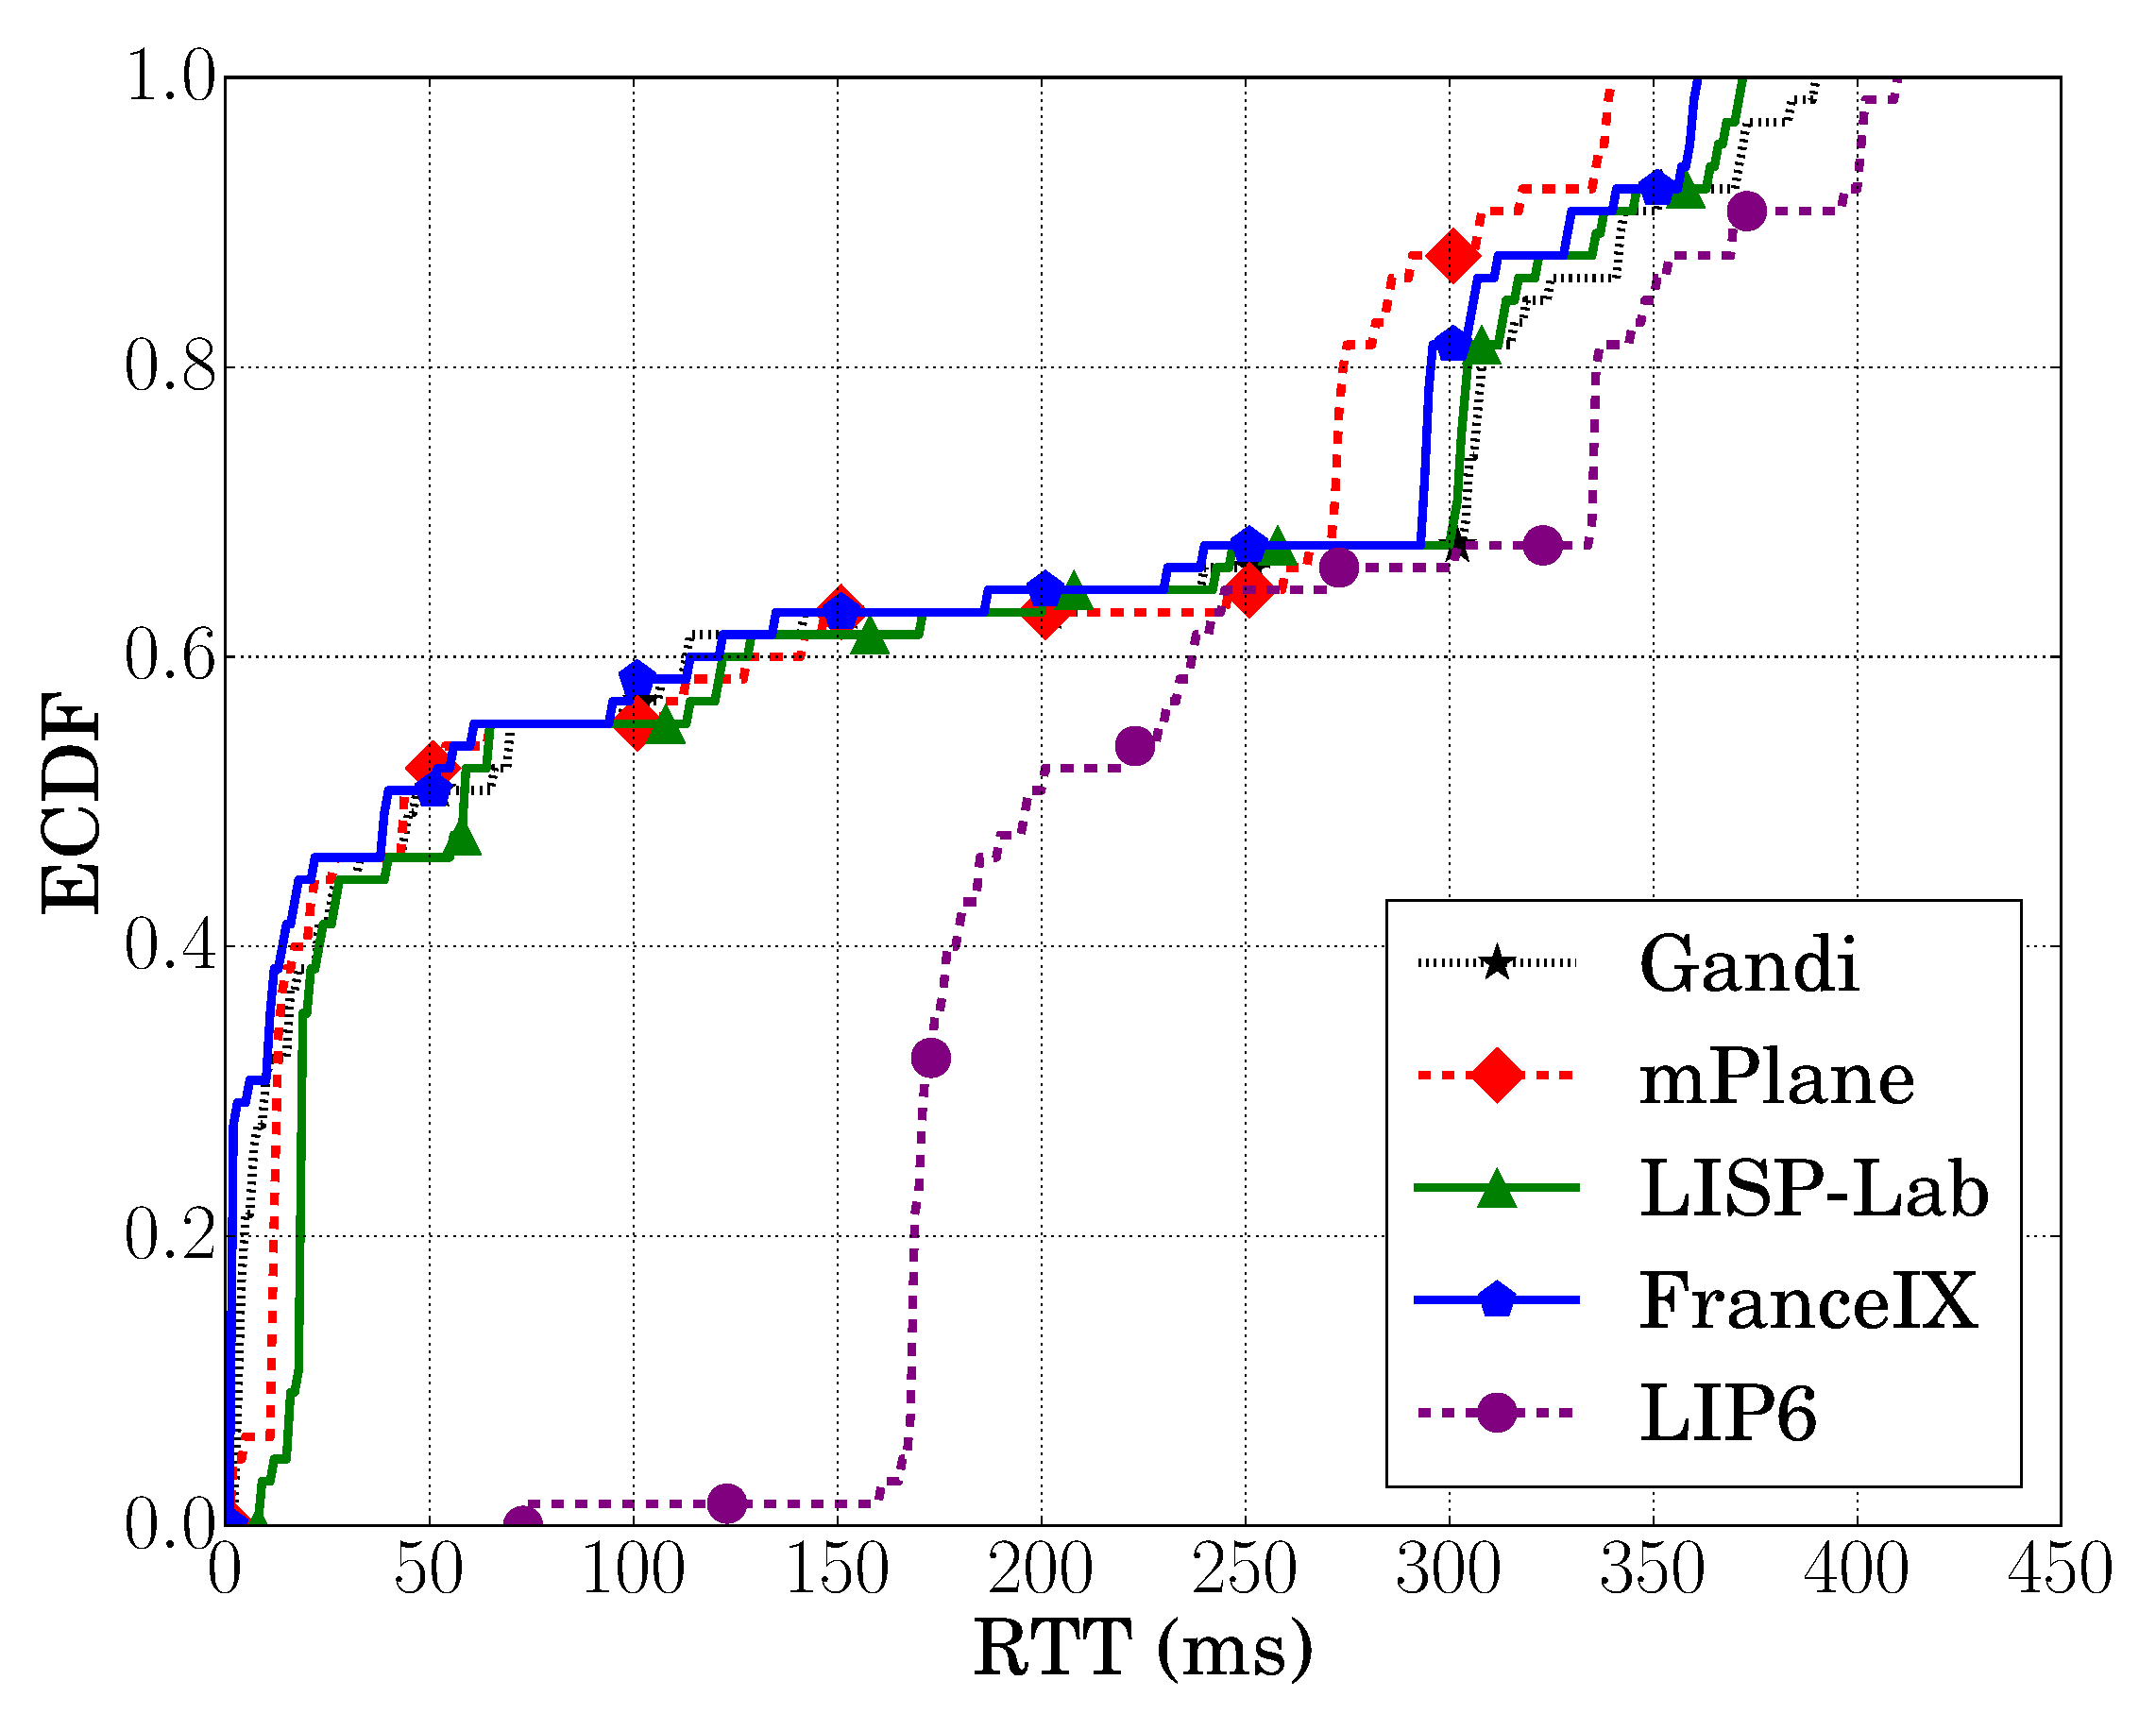
\includegraphics[width=0.6\textwidth]{Pics/v6/CDF_avg(RTT)_median_4_20.eps}
	\caption{CDF of median RTT between different probes (IPv6) from Dataset 2016}
	\label{CDF_of_median_RTT_between_different_probes_v6_2016}
\end{figure}
%-< END FIGURE >--------------------------------------------------------------------

In this section, LISP interworking performance of IPv6 is evaluated with the same metrics as those used in Sec.~\ref{sec:pxtr_ping_v4_2016}.

The CDF of average RTTs to the selected IPv6 destinations is shown on Fig.~\ref{CDF_of_median_RTT_between_different_probes_v6_2016}, which is generally similar to the Fig.~\ref{CDF_of_median_RTT_between_different_probes_v4_2016} for IPv4. The FranceIX anchor still shows the best performance with the smallest delay for almost all the destinations. The RTT of LISP-Lab probe is always higher than the other non-LISP probes with RTT range $[0, 30]ms$ and the difference is around $7 ms$. The RTTs are almost the same when the values are more than $30 ms$. Hence, the performance of IPv6 is similar to IPv4 that the stretch introduced by PxTR is significant when the range of RTT value is small, but can be ignored when the range of RTT value becomes large. 

However, in the experiment for IPv6 targets, the traffic produced by LISP-Lab probe are natively forwarded to the destinations instead of going to the PETR in Lyon first, thus the RTT difference compared to the other non-LISP probes becomes smaller compared to those for IPv4. But the latency still exists, caused by the returning traffic that still need to pass through a PITR. Since the latency decreases, it is easier to be ignored for IPv6. That is the reason why the stretch can be ignored when RTT values are higher than just $30ms$ for IPv6 while it needs to be higher than $200ms$ for IPv4. While the LIP6 probe is always the slowest compared to the other probes, the difference is even $160ms$ to the non-LISP probes and $150ms$ to the LISP-Lab probe. The reason having such a big difference is not only caused by the bidirectional traffic should pass through the PxTR, but also caused by the route between xTR of LIP6 probe to the PETR at Lyon, which has no tunnel indicating the used routing path longer than the case of having an MPLS tunnel. Similar to IPv4, when RTT values are higher than $250ms$, the difference decreases to $40ms$ in most cases.

%-< FIGURE >--------------------------------------------------------------------
\begin{figure}[!t]
	\begin{minipage}[c]{.49\linewidth}
		\begin{center}
			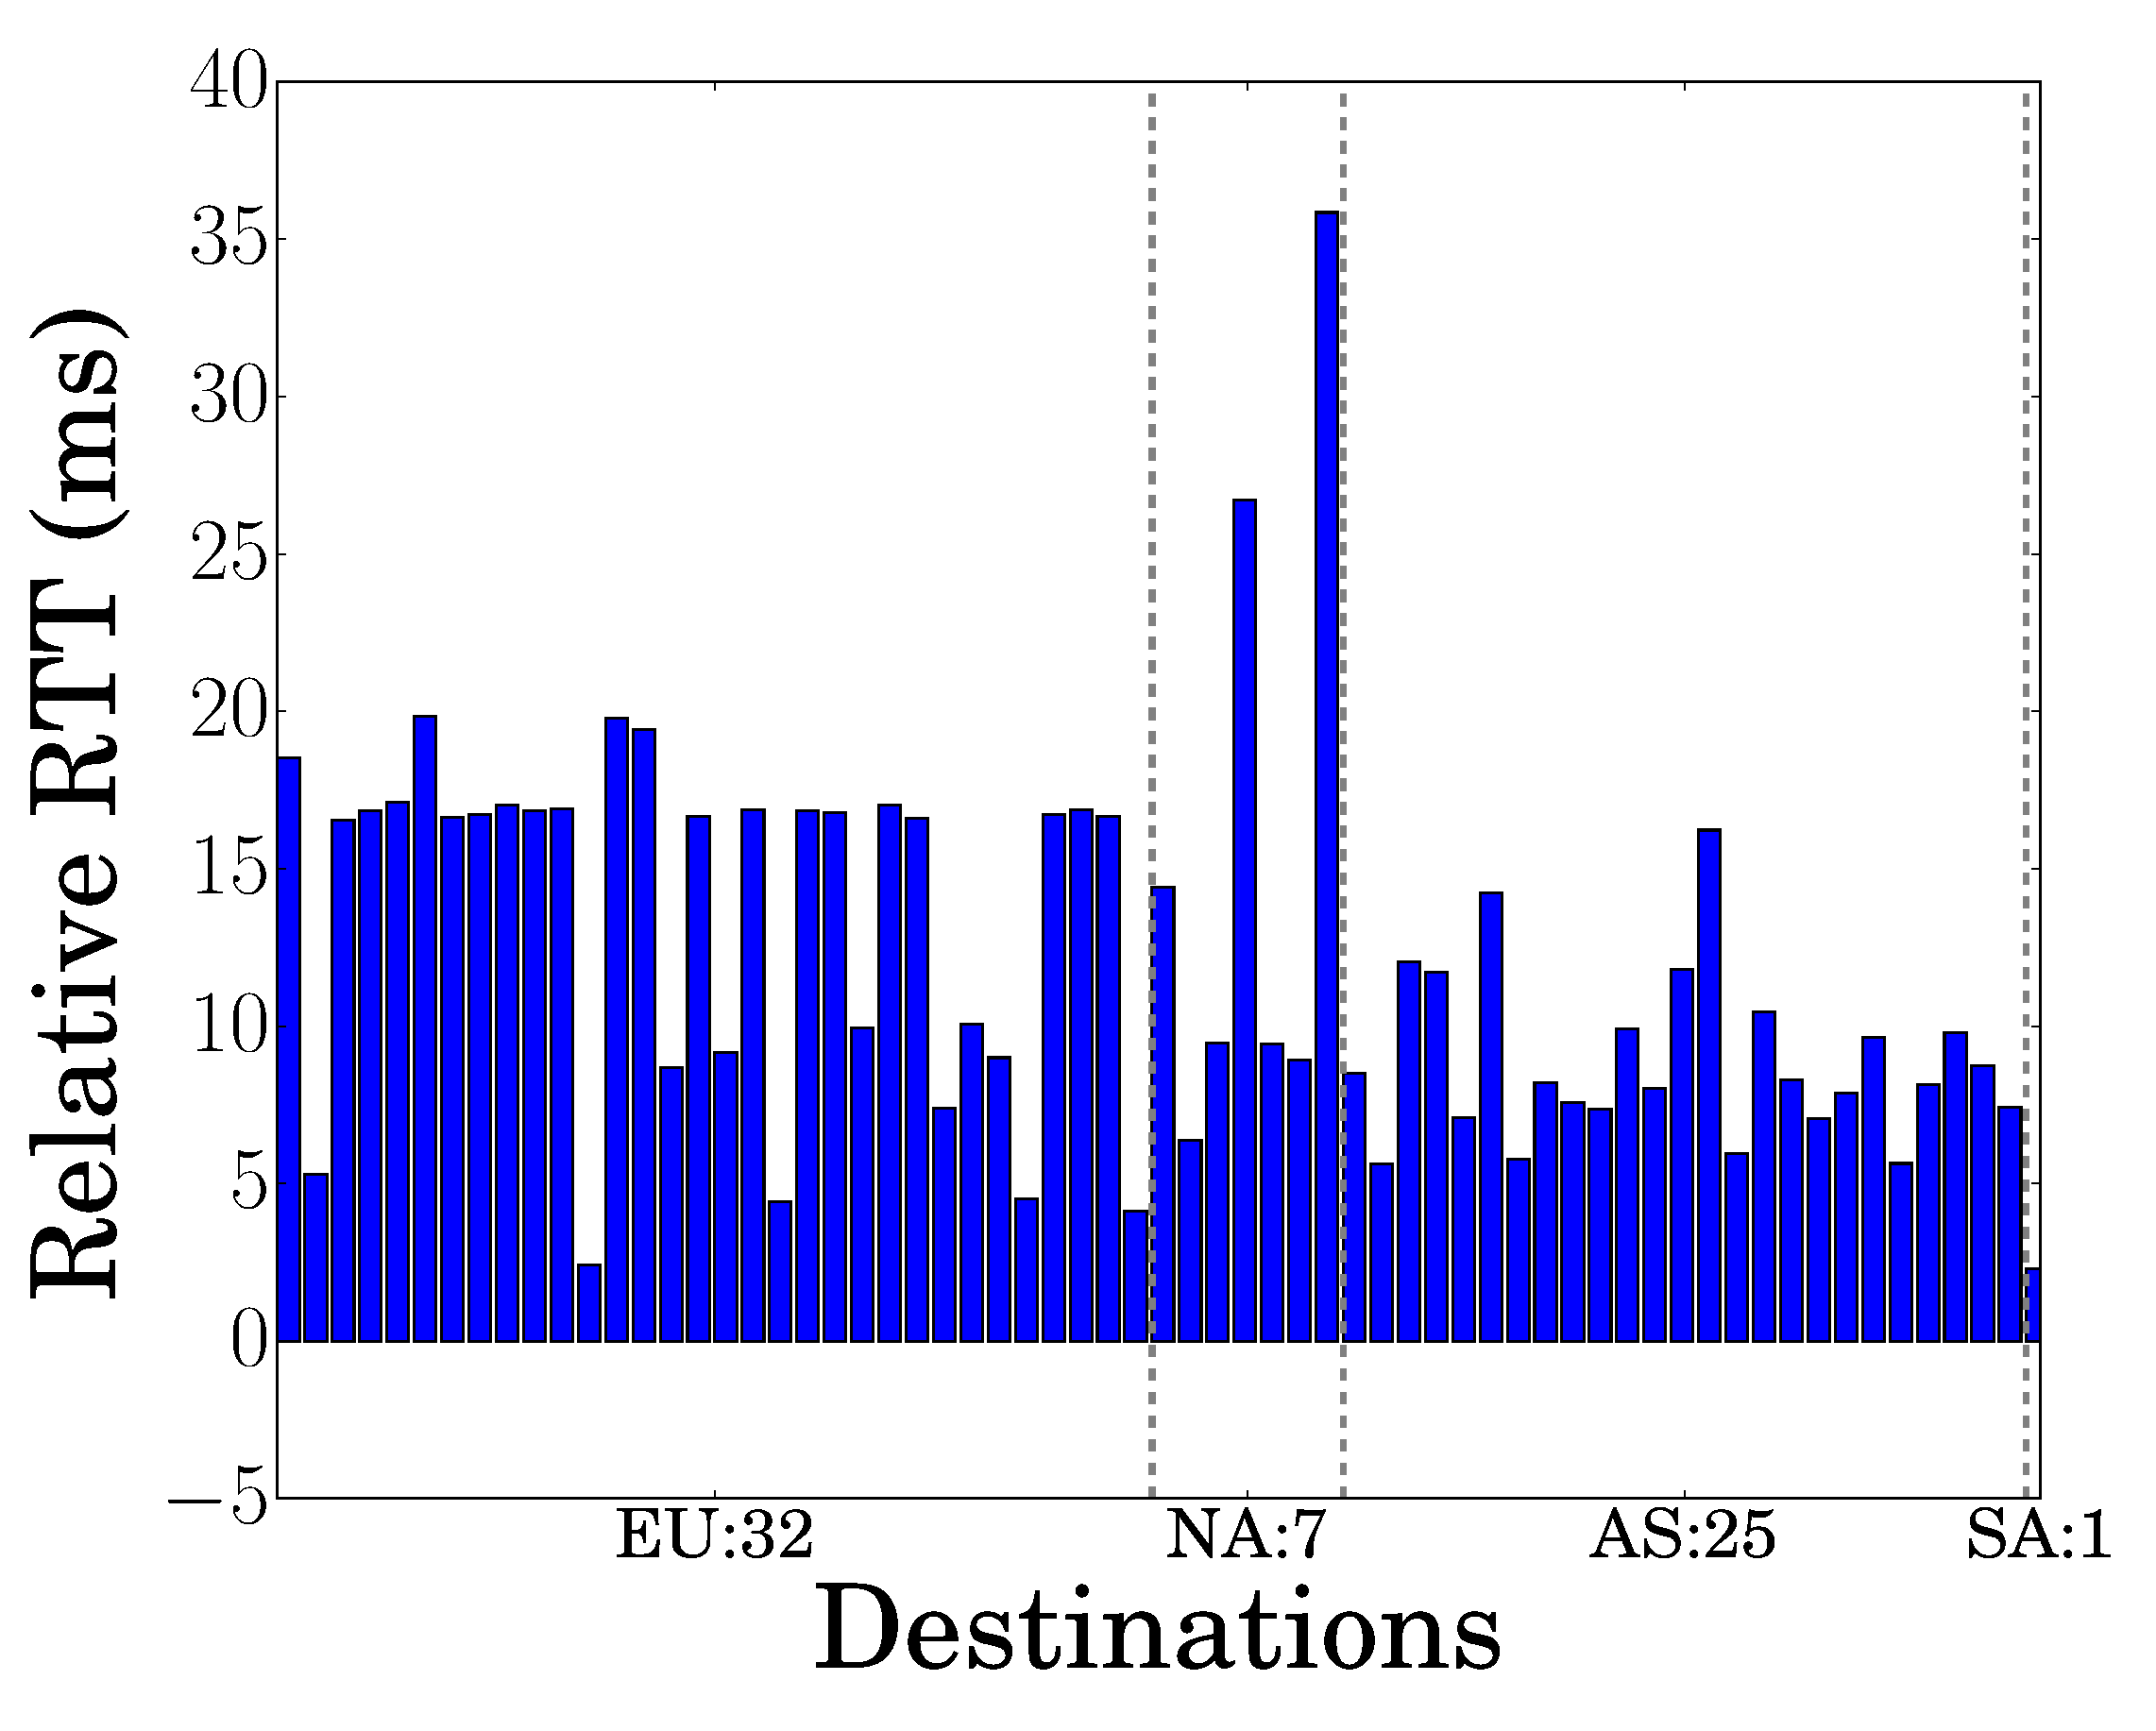
\includegraphics[width=\textwidth]{Pics/v6/Relative_median_avg(RTT)_LISP-Lab-FranceIX.eps}
		\end{center}
	\end{minipage}
	\begin{minipage}[c]{.49\linewidth}
		\begin{center}
			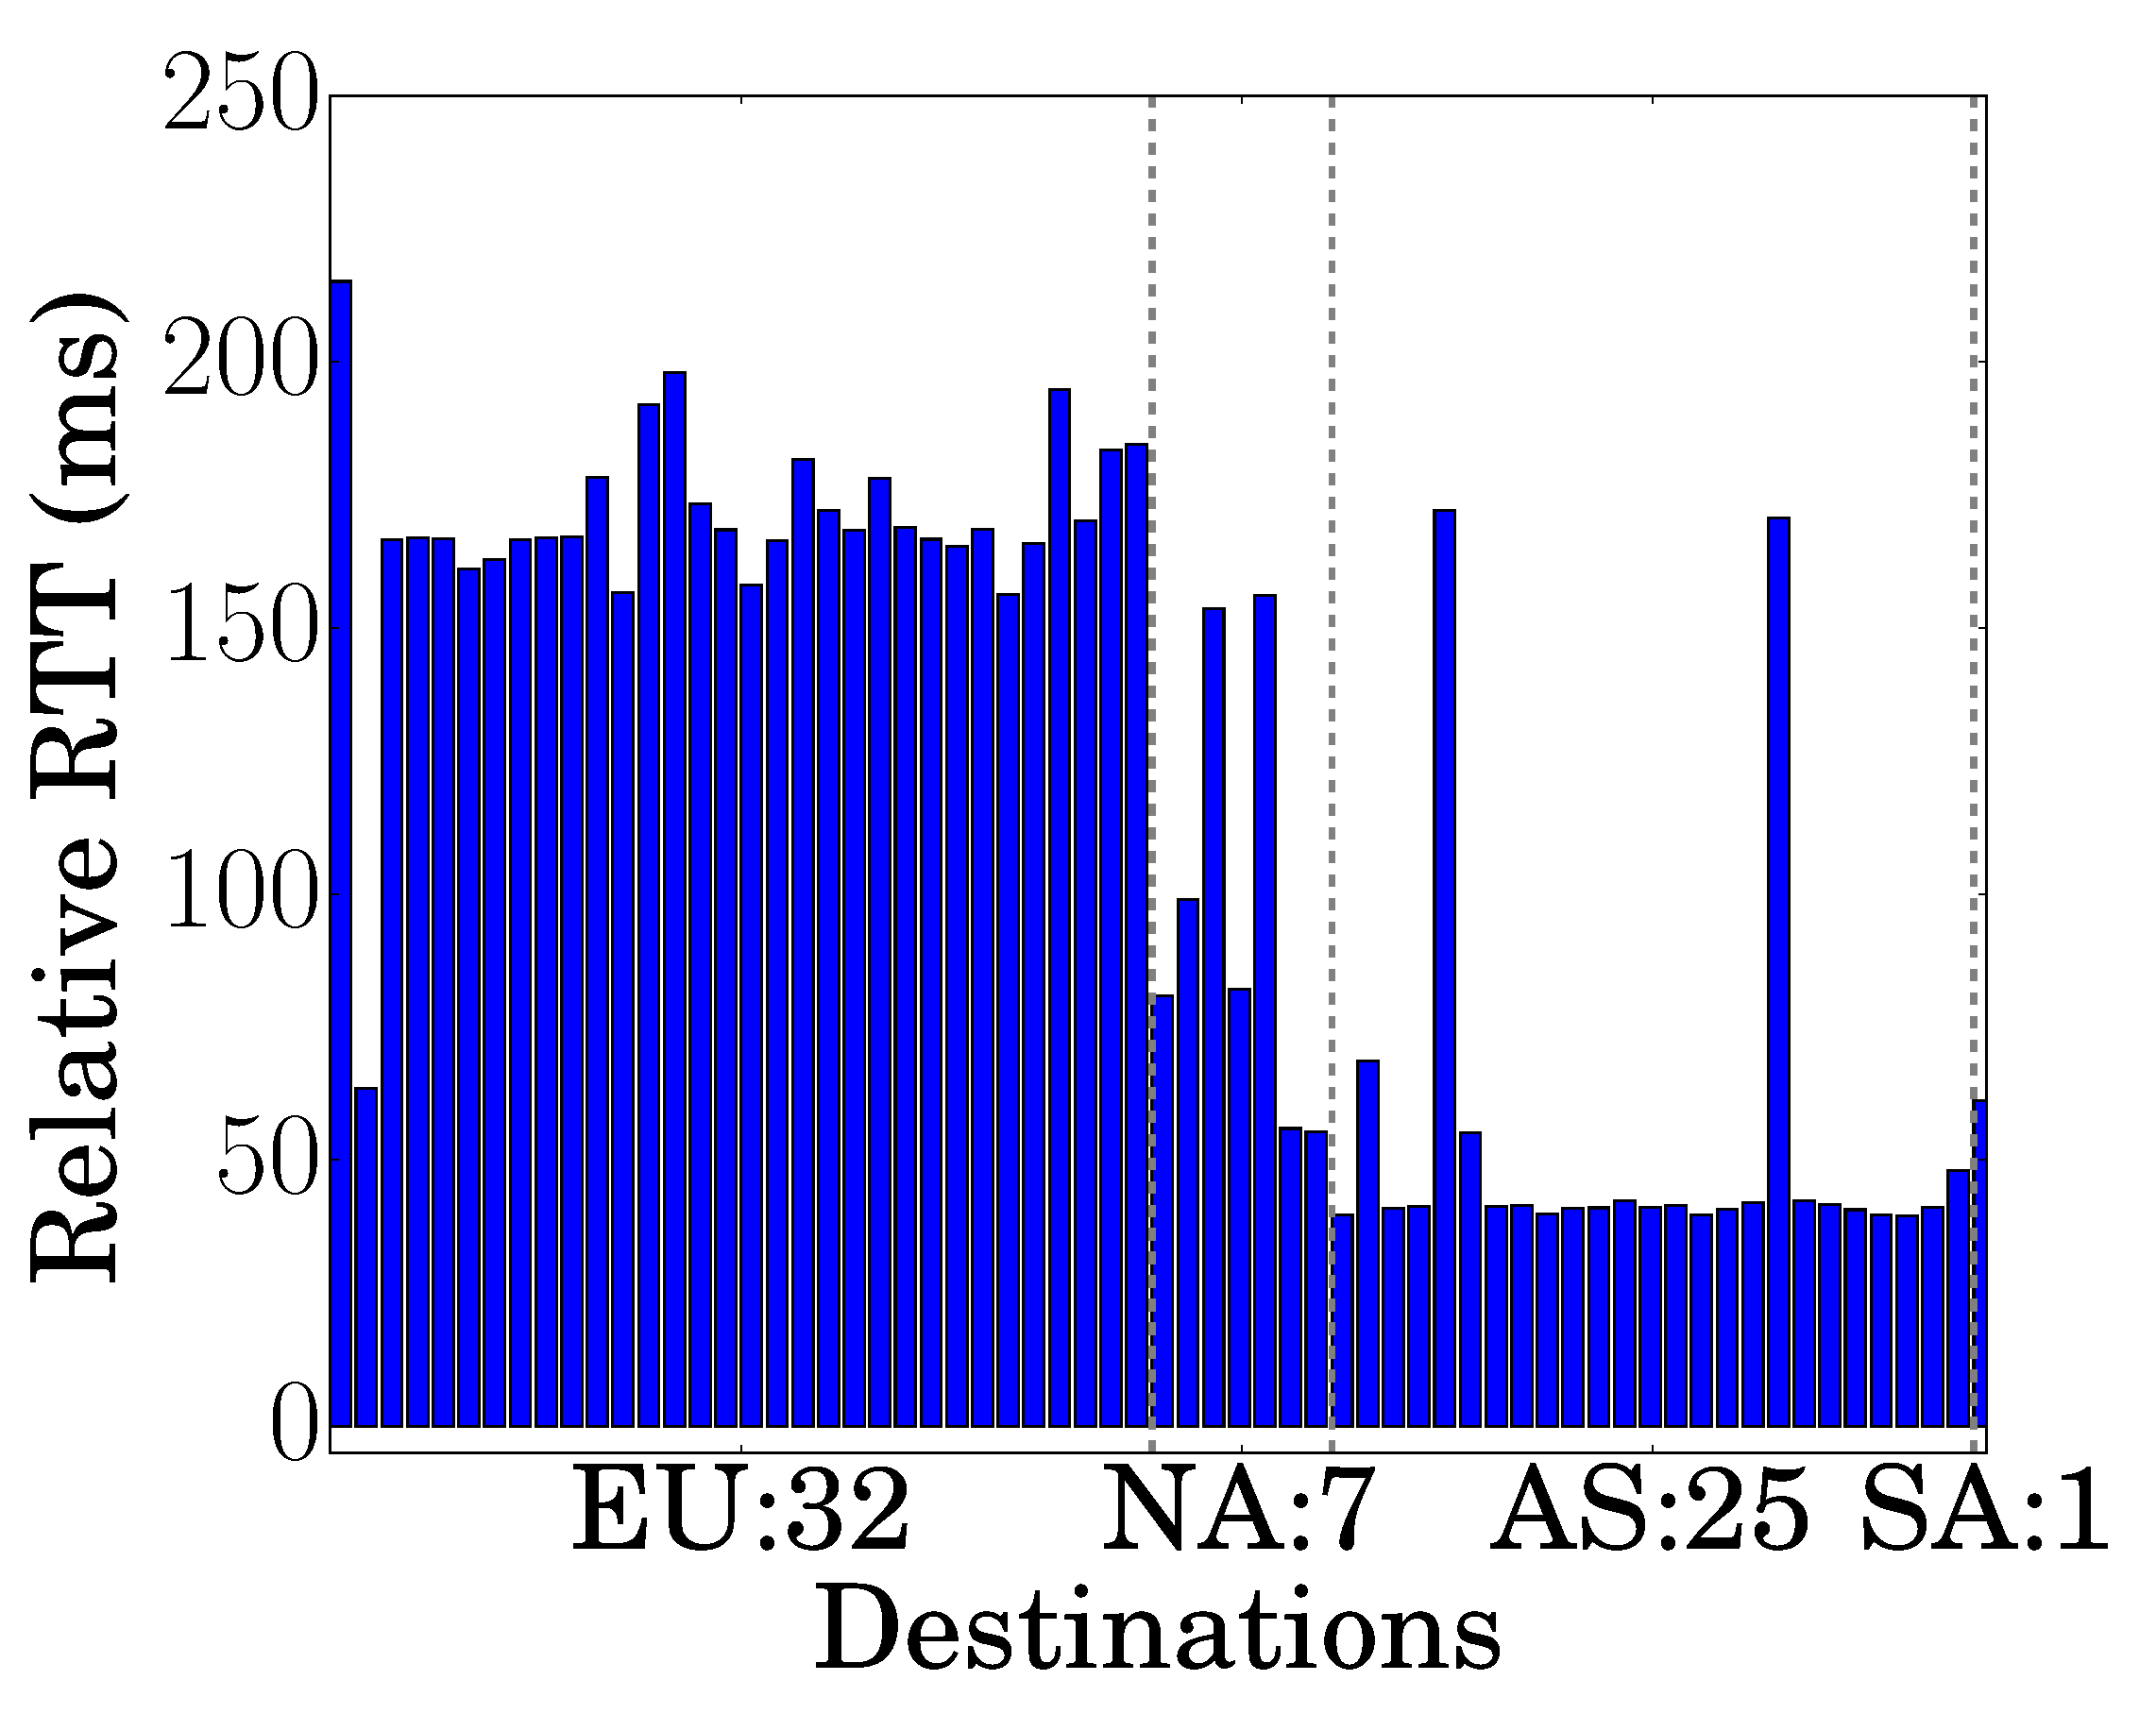
\includegraphics[width=\textwidth]{Pics/v6/Relative_median_avg(RTT)_LIP6-FranceIX_changed_60.eps}
		\end{center}
	\end{minipage}
	\vspace{-0.5mm}
	\caption{IPv6 Relative median RTT clustered by different continents for LISP-Lab (left) and LIP6 (right) from Dataset 2016}
	\label{Relative_median_avg(RTT)_v6_2016}
\end{figure}
%-< END FIGURE >--------------------------------------------------------------------
To further explore why two LISP probes are slower, especially to understand why the LIP6 probe has an extremely large latency compared to the others, we leverage on the Relative RTT between both LISP probes and the FranceIX anchor grouped in four continents as mentioned in Sec.~\ref{sec:pxtr_ping_v4_2016}. In the left figure of Fig.~\ref{Relative_median_avg(RTT)_v6_2016}, which is the relative RTT between LISP-Lab and FranceIX, all the values are positive, indicating that the LISP-Lab probe is slower than the FranceIX anchor no matter to which destination. For the European and North American targets, the relative RTTs are mostly between 5ms and 17ms. But the average relative RTTs decrease to 7ms for the 25 Asian destinations. It proves the fact that for the nearby transmission, the delay introduced by PxTR is significant, while it effects less for the intercontinental transmission to the Asian destinations. What's more, the absolute relative RTT values for IPv6 are smaller than those for IPv4, because there is only returning traffic passing PITR for IPv6 so to reduce the latency. Thus, natively forwarding is faster than using PETR, but not so much. From the Fig.~\ref{Relative_median_avg(RTT)_v6_2016} we also know that there are 32 destinations located in Europe and just 7 in North America. It explains the reason why the curve of CDF for LISP-Lab sharply increases when the RTT is in the small range and mixes with the other non-LISP lines so quickly. It is because a half of destinations are not far away from the probes. Thus, a high percentage (around $50\%$) consists of small RTT values and these RTTs of LISP-Lab have a consistent delay compared to the other non-LISP probes. The mix part is mainly produced by the Asian destinations, to which the RTT values are large and the delay introduced by only the PITR of LISP-Lab is less significant. The relative RTT for the LIP6 probe is shown on the right hand side of Fig.~\ref{Relative_median_avg(RTT)_v6_2016}. The relative RTTs are all positive and much higher, indicating that the LIP6 probe is always quite slower than the FranceIX anchor to whichever target. Especially for the European destinations, the values are around 170ms. But to the North American and Asian targets, the relative RTTs are obviously smaller. As mentioned in Sec.~\ref{sec:pxtr_meth_2016}, the outgoing packets from LIP6 probe still need to go to PETR first and especially the path between its xTR and PETR has no MPLS VPN tunnel. Besides, the main reason that the higher relative RTT values for IPv6 than IPv4 is caused by the LIP6 probe using the PITRs of LISP Beta Network. Different from IPv4~\cite{bgpv4}, there are only two ASes of IPv6 PITRs and both of them are located in US~\cite{bgpv6}. As a result, no matter from which destination, all the returning packets need to pass the PITRs in US first and then forward back to the LIP6 probe located in Paris. By consequence, the relative RTTs to the North American destinations are extremely smaller than those to European destinations. Although the traffic returning back from the Asian destinations also pass through the PITRs in US, the distance between the source and destination is quite far, thus it does not effect a lot to the relative RTTs for Asian targets.

Further, in the $84.61\%$ of cases the FranceIX anchor has the smallest RTT in the IPv6 experiment. The LISP-Lab probe and LIP6 are not the fastest to any destinations, even to the Asian targets. It shows that the LISP performance of IPv6 is a little bit worse than IPv4. Since FranceIX has the smallest RTTs in most situations and as an anchor, its higher measurement capacities lead to its higher stability, we also use the correlation between the RTT of the other 4 probes and FranceIX to see if RTT measurements of each probe are as stable as FranceIX. As shown in Tab.~\ref{correlation_v6_2016}, the correlation coefficient of LISP-Lab is 0.967, which is almost one, indicating although LISP over IPv6 has higher latency than FranceIX caused by the introducing of PxTR, the performance is still stable. However, the correlation coefficient of LIP6 probe is just 0.3734. It is higher than 0.2, but much lower than 0.8, showing that the LIP6 probe is not totally independent from FranceIX, but it has quite low correlation. In fact, the IPv6 RTT series of LIP6 fluctuate a lot over time during the experiment and are not stable.

%%-< FIGURE >--------------------------------------------------------------------
%\begin{figure}[!t]
%	\centering
%	\includegraphics[width=0.5\textwidth]{Pics/v6/Smallest_median_avg(RTT)_proporation.eps}
%	\caption{Smallest median RTT grouped by continent (IPv6)}
%	\label{Smallest_median_avg(RTT)_proporation_v6}
%\end{figure}
%%-< END FIGURE >--------------------------------------------------------------------
%
%%-< TABLE >-----------------------------------------------------------------
%-< TABLE >-----------------------------------------------------------------
%%%%%%%%%%%%%%% Table %%%%%%%%%%%%%%% 
\begin{table}[!tb]
	\centering
	\caption{Correlation coefficient to FranceIX (IPv6) from Dataset 2016}
	\label{correlation_v6_2016}{
	\resizebox{0.7\textwidth}{!}{%
		\begin{tabular}{@{}c|c|c|c|c|c@{}}
			\hline\hline
			& Gandi  & mPlane  & LISP-Lab  & LIP6 &  FranceIX \\ \hline
			Coefficient &  0.9565 & 0.968 & 0.967 & 0.3734 & 1.0     	\\  \hline\hline                 
		\end{tabular}
	}}
\end{table}
%-< END TABLE >-----------------------------------------------------------------

%-< TABLE >-----------------------------------------------------------------
%%%%%%%%%%%%%%% Table %%%%%%%%%%%%%%% 
\begin{table}[!tb]
	\centering
	\caption{Reliability of each probe (IPv6) from Dataset 2016}
	\label{reliability_v6_2016}{
	\resizebox{0.7\textwidth}{!}{%
		\begin{tabular}{@{}c|c|c|c|c|c@{}}
			\hline\hline
			& Gandi  & mPlane  & LISP-Lab  & LIP6 &  FranceIX \\ \hline
			Reliability (\%) &  98.43 & 99.97 & 99.98 & 82.24 & 99.99     	\\  \hline \hline                
		\end{tabular}
	}}
\end{table}
%-< END TABLE >-----------------------------------------------------------------

The Reliability of every probe for IPv6 is almost the same of IPv4 as shown in Tab.~\ref{reliability_v6_2016} except for the LIP6 probe. The higher reliability of LISP-Lab probe than the LIP6 probe confirms again that even for IPv6, the PxTR of LISP-Lab is still more reliable than that of LISP Beta Network, although the latter one has 6 world-wide PxTRs in total, from which only 2 can be used for IPv6. The reliability of LISP-Lab probe for IPv6 is a little bit higher than itself for IPv4, showing that using PxTR may decrease the reliability but the effect is very small. The reliability of the LIP6 probe for IPv6 is also higher than itself for IPv4, indicating that the IPv6 performance of PxTR on LISP Beta Network is better than IPv4, mainly thanks to the use of PxTRs in US. Thus from this comparison, we get a conclusion that the two PxTRs in US are more reliable than the other 4 PxTRs of LISP Beta Network.

The periodicity check for IPv6 is also conducted, but no probes show that their RTT measurements to any destinations have periodicity, either. It indicates that the latency of traffic has no relationship with the specified experiment time, i.e., the RTT measurements generally have the same results regardless the experiment time and duration. Thus, the results of these experiments are not occasional phenomenon with the special results, they are reproducible instead.


%-------------------------------------------- <Subsection> --------------------------------------------
\section{Traceroute-related Results}
\label{sec:pxtr_traceroute} 
% \begin{itemize}[noitemsep,topsep=0pt]
%     \item Distribution of IPv4 relative hops number for LISP-Lab and LIP6
%     \item IPv4 relative hops number clustered by different continents for LISP-Lab and LIP6
%     \item Distribution of IPv6 relative hops number for LISP-Lab and LIP6
%     \item IPv6 relative hops number clustered by different continents for LISP-Lab and LIP6
% \end{itemize}
%%-------------------------------------------- <Subsection> --------------------------------------------
%\subsection{Traceroute-related Results}
%\label{sec:results_traceroute} 
In this section, we use hops number obtained via traceroute from sources (i.e., probes) to destinations as the metric to further evaluate the LISP performance and also further investigate the reasons for the results presented in the ping-related experiments. Since the traceroute can only present the outgoing path, i.e., the routing path from probes to destinations, we focus on the use of the PETR and existence of a VPN between the xTR and the PETR.

When the IPv4 targets are in Europe and America, there are very few cases that the hops number of LISP-Lab or LIP6 is the smallest. Precisely, there is $7.65\%$ of cases that LISP-Lab has the shortest path by hops number to the Asian destinations and $6.63\%$ of cases that LIP6 has the shortest path in the experiment. This result coincides to the percentage of the smallest RTT shown in Fig.~\ref{Smallest_median_avg(RTT)_proporation_v4_2016}.
This consistent relationship between smallest RTT and shortest path exists as well for the IPv6 experiment, where there is no destination at all for which the hop number or the RTT are the smallest (for both LISP-Lab and LIP6 probes). For IPv6, it is FranceIX or Gandi that always have the shortest path to all the targets.

%-< FIGURE >--------------------------------------------------------------------
\begin{figure}[!t]
	\begin{minipage}[c]{.49\linewidth}
		\begin{center}
			\includegraphics[width=\textwidth]{Pics/v4/Relative_hops_num_LISP-Lab-FranceIX_hist_changed_60.eps}
		\end{center}
	\end{minipage}
	\begin{minipage}[c]{.49\linewidth}
		\begin{center}
			\includegraphics[width=\textwidth]{Pics/v4/Relative_hops_num_LIP6-FranceIX_hist_changed_60.eps}
		\end{center}
	\end{minipage}
	\vspace{-0.5mm}
	\caption{Distribution of IPv4 Relative Hops Number for LISP-Lab (left) and LIP6 (right) from Dataset 2016}
	\label{Distribution_v4_relative_hops_num_proporation_LISP-Lab_LIP6}
\end{figure}
%-< END FIGURE >--------------------------------------------------------------------

As FranceIX is always the most stable probe and has the shortest path in most cases, we define \emph{Relative Hops Number (rHN)} clustered by different continents to look at the difference between the hops number of LISP probes and FranceIX. The definition is as: % $Hops Num_{LISP-Lab}$ - $Hops Num_{FranceIX}$ and $Hops Num_{LIP6}$ - $Hops Num_{FranceIX}$. 
\begin{equation}
    \label{rHN_ll_2016}
    rHN_{LL}(d)=HN_{LL}(d) - HN_{F}(d) 
\end{equation}
\begin{equation}
    \label{rHN_l6_2016}
    rHN_{L6}(d)=HN_{L6}(d) - HN_{F}(d) 
\end{equation}
where $d$ is the destination, subscriptions $LL$, $L6$ and $F$ respectively refers to LISP-Lab, LIP6 and FranceIX. The positive value indicates that the hops number of FranceIX is smaller than LISP probes. Fig.~\ref{Distribution_v4_relative_hops_num_proporation_LISP-Lab_LIP6} provides an IPv4 distribution of relative hops number for LISP-Lab on the left and for LIP6 on the right. This figure shows the probability of each relative hops number. For the LISP-Lab probe, the most common relative hops number is 12 with a percentage of $21.77\%$, hence remaining limited in most of the cases. From the ping-related experiment in Sec.~\ref{sec:pxtr_ping_v4_2016} and Sec.~\ref{sec:pxtr_ping_v6} we know that using PxTR introduces some overhead. So the Relative Hops Number being generally positive is reasonable. The very large relative hops number just appears once for 19 and 25, so we regard them as outliers. Similar to the LISP-Lab case, for the LIP6 probe, the most frequent relative hops number is 13 in $19.53\%$ of cases.

%-< FIGURE >--------------------------------------------------------------------
\begin{figure}[!t]
	\begin{minipage}[c]{.49\linewidth}
		\begin{center}
			\includegraphics[width=\textwidth]{Pics/v4/Relative_hops_num_LISP-Lab-FranceIX_changed_60.eps}
		\end{center}
	\end{minipage}
	\begin{minipage}[c]{.49\linewidth}
		\begin{center}
			\includegraphics[width=\textwidth]{Pics/v4/Relative_hops_num_LIP6-FranceIX_changed_60.eps}
		\end{center}
	\end{minipage}
	\vspace{-0.5mm}
	\caption{IPv4 Relative hops number clustered by different continents for LISP-Lab (left) and LIP6 (right) from Dataset 2016}
	\label{v4_Relative_hops_num}
\end{figure}
%-< END FIGURE >--------------------------------------------------------------------

In order to understand where the most common relative hops number appears, we produce the relative hops number for each destination clustered by different continents in Fig.~\ref{v4_Relative_hops_num} to complete Fig.~\ref{Distribution_v4_relative_hops_num_proporation_LISP-Lab_LIP6}. The left figure is for the LISP-Lab probe, indicating that the relative hops number is almost the same for the European and North American destinations and contributes to the relative hops number with high probabilities in Fig.~\ref{Distribution_v4_relative_hops_num_proporation_LISP-Lab_LIP6}. The small relative hops number is mostly produced from the Asian targets. Whereas the outliers are all from the European destinations. The right figure of Fig.~\ref{v4_Relative_hops_num} is for the LIP6 probe, mainly presenting the same result as the LISP-Lab probe, except that the latter rarely has the relative hops number higher than 16, but LIP6 has more.

%-< FIGURE >--------------------------------------------------------------------
\begin{figure}[!t]
	\begin{minipage}[c]{.49\linewidth}
		\begin{center}
			\includegraphics[width=\textwidth]{Pics/v6/Relative_hops_num_LISP-Lab-FranceIX_hist_changed_60.eps}
		\end{center}
	\end{minipage}
	\begin{minipage}[c]{.49\linewidth}
		\begin{center}
			\includegraphics[width=\textwidth]{Pics/v6/Relative_hops_num_LIP6-FranceIX_hist_changed_60.eps}
		\end{center}
	\end{minipage}
	\vspace{-0.5mm}
	\caption{Distribution of IPv6 Relative Hops Number for LISP-Lab (left) and LIP6 (right) from Dataset 2016}
	\label{Distribution_v6_relative_hops_num_proporation_LISP-Lab_LIP6}
\end{figure}
%-< END FIGURE >--------------------------------------------------------------------

With the same evaluation metrics of IPv4, the distribution of Relative Hops Number and the Relative Hops Number clustered by different continents for IPv6 are respectively shown in Fig.~\ref{Distribution_v6_relative_hops_num_proporation_LISP-Lab_LIP6} and Fig.~\ref{v6_Relative_hops_num}. The left figure of Fig.~\ref{Distribution_v6_relative_hops_num_proporation_LISP-Lab_LIP6} presents that the most common relative hops number between the FranceIX anchor and the LISP-Lab probe is 7 in $56.72\%$ of cases, more than a half, much higher than the probability of other relative hops numbers. The range of relative hops number is smaller compared to IPv4 and the most common relative hops number is also smaller, since the traffic does not need to pass the PETR, but is just natively forwarded so the overhead is reduced. The left figure of Fig.~\ref{v6_Relative_hops_num} reveals the truth that 7 relative hops numbers are produced by the majority of targets regardless where the destinations are, instead of like the one of IPv4, where the relative hops number for European and American destinations are more than the Asian's. As the relative hops number from PETR is only 3, but 7 for natively forwarding, it is likely that the PxTR has shorter paths to most destinations, leads to the decreasing of hops number for the LISP-Lab probe. The relative RTTs higher for European and American destinations than those for Asia shown in left figure of Fig.~\ref{Relative_median_avg(RTT)_v6_2016} are mainly caused by the returning path, since it is natively forward for outgoing and there is no difference by continents. For IPv6, the LIP6 probe has extremely high relative hops number in a range from 12 to 24. The majority of relative hops number is 23 in $19.57\%$ of the cases and followed by 13 with a percentage of $17.39\%$. The higher relative hops number is caused by not using the VPN between xTR and PETR compared to the IPv4 case. The right figure of Fig.~\ref{v6_Relative_hops_num} visualizes the 23 relative hops number coming from the European destinations and 13 coming from the Asian targets. The form coincides to the relative RTT for IPv6 shown in the right hand part of Fig.~\ref{Relative_median_avg(RTT)_v6_2016}, indicating that the high relative RTTs are caused by the high relative hops number. 

Concerning the RTT performance of the LISP-Lab probe to Asian destinations, which sometimes shows even better than FranceIX, we analyze the AS-path (Autonomous System path) from FranceIX and LISP-Lab to Asian destinations that the packets traverse. Since all the IPv4 packets from LISP-Lab probe are sent to PETR at Lyon first, so the AS-path discussed in the followings is actually from PETR to the Asian destinations. By comparing the AS-path, we find that FranceIX and LISP-Lab very often take different paths, with only the last 1 or 2 hops in common. Even further, by looking at the geographic location of each hop of \emph{traceroute}, it can be observed that FranceIX and LISP-Lab take the path even in the different directions in most of the cases. In particular, there are 11 destinations out of 117 in total (i.e., 9.4\%) for which the packets sent by LISP-Lab pass through US, while the packets sent by FranceIX pass through Eastern Europe. There are 68 destinations (i.e., 58.1\%), which show exatly the opposite situation, i.e., packets sent by FranceIX pass through US, while packets sent by LISP-Lab pass through Eastern Europe. This last case is when LISP-Lab has smaller RTT (compared to FranceIX), almost all of the times (with only few exceptions). 

%-< FIGURE >--------------------------------------------------------------------
\begin{figure}[!t]
	\begin{minipage}[c]{.49\linewidth}
		\begin{center}
			\includegraphics[width=\textwidth]{Pics/v6/Relative_hops_num_LISP-Lab-FranceIX_changed_60.eps}
		\end{center}
	\end{minipage}
	\begin{minipage}[c]{.49\linewidth}
		\begin{center}
			\includegraphics[width=\textwidth]{Pics/v6/Relative_hops_num_LIP6-FranceIX_changed_60.eps}
		\end{center}
	\end{minipage}
	\vspace{-0.5mm}
	\caption{IPv6 Relative hops number clustered by different continents for LISP-Lab (left) and LIP6 (right) from Dataset 2016}
	\label{v6_Relative_hops_num}
\end{figure}
%-< END FIGURE >--------------------------------------------------------------------


%-< SECTION >--------------------------------------------------------------------
%\section{LISP-related Discussion and Conclusion}
\section{Summary}
\label{sec:pxtr_conclusion}
% \begin{itemize}[noitemsep,topsep=0pt]
%     \item PxTR indeed introduces the negative effects for the near destinations, but can be ignored for the intercontinental long-distance transmission.
%     \item Position of PxTR is very important.
%     \item LISP is generally stable, except for the IPv6 performance of LISP Beta Network.
%     \item LISP-Lab PxTR is more reliable than the ones of LISP Beta Network.
%     \item Encapsulating into LISP packets has only 4 hops more compared to the packets being natively forward by xTR.
% \end{itemize}
% In the last years, the Locator/ID Separation Protocol (LISP) has gained attention as promising solutions of several scaling issues the Internet is facing. Various inter-operable implementations, and deployment exist, however, to promote the growth of this relatively novel technology and improve its performance, it requires large scale measurements in real deployments. 
In this chapter, we conduct a six-hours as well as a two-weeks real network measurements with LISP Beta Network, LISP-Lab platform and RIPE Atlas to provide a comprehensive performance evaluation of LISP interworkings. Concretely, we provide a first thorough sight on the performance of LISP PxTR. Since the results of experiment in 2016 coincides to the one in 2015 and are more comprehensive. Thus, we conclude this chapter by presenting the observations of the Dataset 2016. 

In our large scale measurement campaign, we take into account 5 probes as sources, 500 IPv4 and 122 IPv6 addresses as destinations, conducting ping and traceroute experiments. We find that the PxTR indeed introduces the negative effects for the destinations located in Europe and America, but the negative impact of PxTR can be ignored for the intercontinental long-distance transmission to Asia destinations. From the experiment, the results show that the position of PxTR is very important. The PxTR either near to the sources or the destinations can decrease the latency a lot. Generally speaking, LISP is stable compared with the reference anchor FranceIX, except for the IPv6 performance of LISP Beta Network. Further, the performance of LISP-Lab PxTR is more reliable than the one of LISP Beta Network, although the latter has 6 worldwide PxTRs used for IPv4 and 2 located in US used for IPv6, whereas LISP-Lab has only 1 PxTR for both IPv4 and IPv6. Compared to leveraging on PxTR, natively forwarding without using LISP decreases the latency, but not much. The traceroute experiment shows that introducing PxTR of course brings more hops, but if the PETR is well configured, so to always have peers to the destinations, there are only 4 more hops compared to the packets being natively forward by xTR without encapsulating with LISP.
 % Measurement on PxTR
%*******************************************************************************
%****************************** Sixth Chapter *********************************
%*******************************************************************************

\chapter{ns-3 Implementation of LISP and LISP-MN}
\label{cha:ns-3}

% **************************** Define Graphics Path **************************
\ifpdf
    \graphicspath{{Chapter7/Pics/Raster/}{Chapter7/Pics/PDF/}{Chapter7/}}
\else
    \graphicspath{{Chapter7/Pics/Vector/}{Chapter7/}}
\fi

%-< ABSTRACT >--------------------------------------------------------------------
The \emph{Locator/Identifier Separation Protocol} (LISP) reconstructs the current IP addressing space to improve the scalability and no interrupt mobility issues. LISP Mobile Node (LISP-MN) is based on the basic LISP functionality to provide seamless mobility across networks. The basic LISP architecture is deployed on LISP Beta Network and LISP-Lab platform to offer the researchers a realistic experimental environment, but both do not support LISP-MN. Some simulation models with LISP extensions are implemented on various simulators, but are unfortunately not open source. Providing a free and flexible simulation model with the basic LISP architecture as well as the extensions so to help researchers quickly test new LISP behaviors motivates our work. This paper introduces the implementation of the basic LISP architecture model and LISP-MN on the simulator ns-3. It also provides the evaluation results in mobility scenario to validate the model and shows when the current proposal of LISP-MN is behind a LISP-site has a very high delay during the handover procedure.

The rest of chapter is organized as follows: Sec.~\ref{sec:ns3_intro} reviews LISP architecture, highlighting the LISP mobility mechanism; Sec.~\ref{sec:ns3_related_work} ... Sec.~\ref{sec:ns3_modify} analyzes the design and implementation of our prototype, and afterwards, Sec.~\ref{sec:evaluation} presents preliminary evaluation results of our implementations. We finish with a discussion and some ideas for future work.
%-< ABSTRACT >--------------------------------------------------------------------

\section{Introduction}
\label{sec:ns3_intro}
% The research community are on the need of an open source LISP/LISP-MN simulator to facilitate the LISP-related studies. There exist some research efforts to fulfill this gap, however these simulators are not available for the pubic neither covering LISP-MN. That's the motivation of this work and importance of our work.
% \begin{itemize}
%     \item present the shortcomings of measurements on the real Internet and thus the advantages of simulation
%     \item xx
% \end{itemize}
The \emph{Locator/Identifier Separation Protocol} (LISP)~\cite{rfc6830} is initially proposed to solve the scalability and flexibility issues of current Internet architecture, since it decouples the Routing Locators (RLOCs) and Endpoint Identifiers (EIDs). This allows that the BGP routing tables in Internet core just announce the globally routable RLOCs whereas EIDs are only locally used within the subnets. LISP is under standardization at the IETF around ten years and as it develops, more advantages are found, such as: seamless mobility at terminal or in the Data Center, IPv6 transition and traffic engineering~\cite{saucez2016locator}. Among them, the continuous communication without interruption during the handover of terminals becomes a hot topic recently.

To test the various features of LISP, two LISP testbeds are built: LISP Beta Network and LISP-Lab platform. But both of them are only the basic LISP architectures and do not support mobility functionality. Some platform-specific LISP implementations, such as: OpenLISP~\cite{phung2014openlisp}, Open Overlay Router (OOR)~\cite{LISPmob} and Cisco's implementation~\cite{CiscoIOS}, can provide realistic LISP evaluations but lack the flexibility to test the new features. A LISP simulator is a good choice for the researchers. To the best knowledge, LISP is first implemented on ns-3~\cite{ns3}, which is widely used by academic researchers and educational use in~\cite{lezama2009implementation}, but mobility support is not included as well. While within OMNET++ platform, LISP and mobility features are implemented~\cite{klein2012integration}. However, their source code is not available online. To promote the development of LISP and as ns-3 gradually shows the potential to take the momentum in network simulator domain~\cite{rana2017implementation}, it highlights the importance to implement LISP and its mobility extensions under ns-3 and motivates our work.

In this paper, we introduce the implementation of basic LISP functions and mobility features on ns-3 by both modifying the existent ns-3 modules and integrating the new modules. Our simulator is validated by achieving a mobility scenario, in which a terminal changes the attachment points by keeping the communication with the remote node. All the handover procedures are transparent to the terminal, however, the delay to receive the packets again presents high.

\section{Related work}
\label{sec:ns3_related_work}
%-< SUB SECTION >--------------------------------------------------------------------
% \subsection{Description of ns-3}
% \label{sec:descriptionns-3}
 ns-3~\cite{ns3} is a popular and free discrete-event network simulator for networking research. To be closer to the real implementation (in a real Operating System), easily include C-based implementation codes, ease debugging and reduce the cost on maintaining in a long term, C++ is prioritized to be the unique programming language for ns-3. Besides, ns-3 offers the possibility to visualize the simulation instance so to allow the users to visually confirm the packets flow as they expect.
%\begin{itemize}
%    \item Description of ns-3.
%    \item The simulator supporting LISP is introduced in Sec.~\ref{subsec:implementation_OMNet}.
%\end{itemize}


%%-< SECTION >--------------------------------------------------------------------
%\section{Simulation model}
%\label{sec:sim_model}


%-< SECTION >--------------------------------------------------------------------
\section{LISP/LISP-MN Implementation based on ns3}
\label{sec:ns3_modify}
It should be noted that this work is based on a prior implementation work by Lionel. However, his implementation has no support for LISP MN.

%-< FIGURE >--------------------------------------------------------------------
\begin{figure*}[!t]
	\centering
	\includegraphics[width=\textwidth]{Pics/LISP-NS3-UML}
	\caption{UML diagram of LISP/LISP-MN implementation. The solid arrow refers to a composition relation, while the blank one refers to a inheritance relation.}
	\label{LISP-UML}
\end{figure*}
%-< END FIGURE >--------------------------------------------------------------------
Our implementation is under ns-3.26 and based on LISP~\cite{ietf-lisp-rfc6830bis-03} and LISP-MN standards~\cite{meyer-lisp-mn-16}. The main classes are shown in Fig.~\ref{LISP-UML} in form of UML diagram. The blank blocks refer to the classes that we added into ns-3, while darker blocks are classes already in ns-3. As a design choice, we implement LISP/LISP-MN functionalities by modifying and extending the \emph{internet} module of ns-3, instead of creating a new independent module. The justification of this design is that LISP/LISP-MN and legacy internet module have an interdependent relationship. However, this kind mutually dependent relationship between modules is not supported by ns-3. Inspired from design of OpenLISP~\cite{saucez2009openlisp}, the Data Plane implementation is in "kernel space" (i.e. ns-3's \emph{TCP/IP stack}) and Control Plane is implemented in "user space" (i.e. ns-3 \emph{Application}). The communication between LISP Data and Control Plane is developed via a dedicated socket (i.e. \emph{LispMappingSocket}) that inherits from ns-3 \emph{Socket} class. It should be noted that our implementation only supports IPv4 at time of this writing. The IPv6 support (i.e. the implementation related to IPv6 such as \emph{LispOverIpv6Impl}) is still in process.  

%-< SUB SECTION >--------------------------------------------------------------------
\subsection{Implementation of LISP Data Plane}
\label{subsec:modifyInternet}
%\begin{itemize}
%    \item Modification of Receive method
%    \item Modification of Delivery method
%    \item Implementation of LISP encapsulation and decapsulation
%\end{itemize}
A LISP-compatible node (terminal or router) should be capable of determining whether a packet should be passed to LISP-related procedure and retrieving the associated mapping information if necessary. To this end, a new class called \emph{LispOverIp} and its extended classes (refer to Fig.~\ref{LISP-UML}) are added to ns-3 \emph{internet} module. This class is in charge of checking whether necessary to do LISP-related operations (\emph{NeedEncapsulation()}, \emph{NeedDecapsulation()}), and encapsulating conventional IP packets (i.e., \emph{LispOutput()}) as well as decapsulating LISP packets(\emph{LispInput()}). It also contains a smart pointer pointing to the LISP database and LISP cache. Both data structures (store the EID-RLOC mapping information) are represented by class \emph{SimpleMapTable} that inherits from \emph{MapTable}. The inheritanc mechanism allows other users to implement their own implementation of LISP database and cache. To support LISP functionalites, the \emph{Ipv4L3Protcol}, which is the IP layer implementation in ns-3, contains one \emph{LispOverIp} object and \emph{Ipv4L3Protcol}'s packet transmission and reception procedures are accordingly adapted.

To process outgoing packets, the adapted \emph{send()} in \emph{Ipv4L3Protcol} first verifies whether the \emph{LispOverIp} object is present. If yes, some checks are then conducted to determine that this packet should be processed by \emph{LispOutput()} (to encapsulate the packets) or by conventional packet transmission routine. For example, if both source and destination IP address of this packet belong to the same network, the LISP-related process (e.g., encapsulation) is skipped and this packet is processed as in a non-LISP network. Otherwise, EID-RLOC mapping information is searched from LISP cache and LISP database on LISP-MN node. In case of cache missing (i.e. destination RLOC is not found in the cache), the packet is dropped and \emph{SendNotifyMessage()} in \emph{LispOverIp} notifies the \emph{LispEtrItrApplication} that runs on LISP-MN node via a \emph{LispMappingSocket} socket. Once reception of cache missing event from LISP Data Plane (i.e. \emph{LispOverIp} object), \emph{LispEtrItrApplication} initiates a Map-Request message to LISP mapping system. Once reception of Map-Reply, the received EID-RLOC mapping is inserted into LISP cache. It should be noted that as an implementation choice, before the reception of Map-Reply message, all transmitted packets with the required RLOC as desination are dropped. One can also design a buffer to queue these packets and resend them once the required mapping informtion is received via Map-Reply. The advantage of such an implementation is to reduce the packet loss rate. 

For an incoming packet, if the destination of this packet is the node itself, the packet is processed by \emph{LocalDelivery} method in \emph{Ipv4L3Protocol}. Before passing to transport layer, \emph{LocalDelivery} checks if the packet should be decapsulated. If yes, it is passed to \emph{LispInput} method, in which the packet is decapsulated and reinjected in the IP stack. If the received packet destination is not this node, this packet is processed by patched \emph{IpForward} method. This packet may be ended up with LISP encapsulation procedure.

%-< SUB SECTION >--------------------------------------------------------------------
\subsection{Implementation of LISP Control Plane}
\label{subsec:control-plane-impl}
%\begin{itemize}
%    \item Implementation of xTR under ns3
%    \item Implementation of MS under ns3
%    \item Socket communication between control plan and data plan
%\end{itemize}
The implementation of LISP Control Plane at least should provide ITR/ETR, MR and MS. In practice, ETR and ITR functionalities are usually placed on a same router. In our implementation, they are included into classs \emph{LispEtrItrApplication}. A ns-3 node that runs \emph{LispEtrItrApplication} is a LISP-compatible router. It should be able to communicate with \emph{LispOverIp} on the same node (e.g. inform cache missing event) and other LISP-compatible routers (e.g. Map-Request/Map-Reply). To support LISP-MN feature, \emph{LispEtrItrApplication} also communicates with DHCP client application. For example, once a LISP-MN obtains an IP address from DHCP server, \emph{LispEtrItrApplication} receives the corresponding EID-RLOC mapping and sends a Map-Register message~\cite{meyer-lisp-mn-16}.

A node that runs a \emph{MapServer} application is the MS in a LISP-supported network. This class maintains a LISP database to store the EID-RLOC mapping information, learned from Map-Register message at the initialization stage. In current implementation, the role of MR is to receive the Map-Request message from xTR and forward it to the MS.

%-< SUB SECTION >--------------------------------------------------------------------
\subsection{Integration of TUN net interface card}
\label{subsec:tundevice}
To support mobility, LISP-MN actually can be regarded as a small LISP-Site, in which xTR functionalities and DHCP service are implemented, as well as configured address of MR and MS. As a LISP-MN node, it has a static permanent EID and dynamic RLOC assigned by the DHCP server. To differentiate with conventional RLOC of xTR interface, such kind of RLOC is referred to as the local RLOC (LRLOC). Different from conventional LISP node, at least two net interface cards (NIC) are installed into LISP-MN. One is \emph{WifiNetDevice}, the other is a TUN type card. The DHCP client application runs on LISP-MN's \emph{WifiNetDevice} and thus the LRLOC is allocated to this card. The permanent EID is assigned to \emph{VirtualNetDevice} net card. We modify the node's routing table so that each packet's inner header contains IP address on \emph{TunNetDevice} and outer header contains IP address of \emph{WifiNetDevice} as source address.

%-< SUB SECTION >--------------------------------------------------------------------
\subsection{Integration of DHCP}
\label{subsec:DHCP}
%\begin{itemize}
%    \item LISP-MN, in case of IPv4, need the intervention of DHCP procedure
%    \item The current version of DHCPv4 is not compatible with LISP
%    \item Implementation of LISP-compatible DHCPv4 based on conventional DHCPv4
%\end{itemize}
To support mobility within conventional LISP node, a modified DHCP client application is integrated into ns-3 node. To be compatible with LISP functionality, DHCP client application is modified. Once the DHCP client receives an allocated IP address (i.e. LRLOC), it notifies the \emph{LispEtrItrApplication} (i.e. LISP Control Plane) by sending a dedicated message that contains the EID-LRLOC mapping. \emph{LispEtrItrApplication} is in charge of populating the received mapping entry into LISP database. During the mobility process, when wireless link is down, the DHCP client flushes the LISP-MN database and populates the database again once reception of new LRLOC. 

% To support DHCP, conventional LISP-related process is also modified. For example, to transmit a DHCP Discovery message (application layer message), its source IP address is set as $0.0.0.0$. This message should be not processed by and should not passed to \emph{LispOutput} in \emph{LispOverIp}.


%-< SECTION >--------------------------------------------------------------------
\section{Evaluation}
\label{sec:ns3_evaluation}
We validate our LISP/LISP-MN implementation by conducting a simulation and providing a preliminary performance evaluation of handover delay. The simulation topology is shown in Fig.~\ref{sim_scenario}.
%-< FIGURE >--------------------------------------------------------------------
\begin{figure}[!th]
	\centering
	\includegraphics[width=0.5\textwidth]{Pics/mobility_through_subnets_2_encap_topo}
	\caption{LISP mobility simulation scenario for double encapsulation}
	\label{sim_scenario}
\end{figure}
%-< END FIGURE >--------------------------------------------------------------------

%-< SUB SECTION >--------------------------------------------------------------------
\subsection{Simulation Setup}
\label{subsec:ns3_setup}
%\begin{itemize}
%    \item Topology of simulation setup
%    \item The simulation parameter settings
%\end{itemize}
In our simulation, a LISP-MN with permanent EID 172.16.0.1 is initially placed in network 10.1.1.0/24. An \emph{echo} application on LISP-MN sends one packet per second to a remote stationary node CN with EID 10.3.3.2, and the LISP-MN moves into network 10.1.7.0/24 at speed of $7.07m/s$. The distance between xTR\_1 and xTR\_2 is $170m$. LISP-MN node uses Wi-Fi to connect to xTR\_1. At a certain moment during the moving, the Wi-Fi link between LISP-MN and xTR\_1 is down, which triggers the handover procedure. Afterwards, LISP-MN connects to xTR\_2 and reestablishes the communication with CN node. The total simulation time is set to $45s$ and the DHCP procedure delay is set to $1s$. We conduct many times of simulations with the various beacon interval of Wi-Fi channel in the range of $0.05s$ to $2s$.

%-< SUB SECTION >--------------------------------------------------------------------
\subsection{Results}
\label{sec:ns3_results}
%\begin{itemize}
%    \item Show that LISP-MN procedure passes successfully
%    \item Show that the handover delay in LISP-MN handover procedure
%\end{itemize}
As shown in Fig.~\ref{sim_schema}, when MN sending the packets to CN during the simulation, it needs double encapsulation and the packet flow sequences are as follows. The traditional IP packets with EID 172.16.0.1 as source address and EID 10.3.3.2 as destination address are encapsulated by adding Local RLOC 10.1.1.1 as outer source address and RLOC 10.1.5.2 as outer destination address after MN querying the mapping information to MR. The LISP packets are encapsulated and forwarded to xTR\_1. The latter gets the mapping information from MR and encapsulates the packets again by adding the RLOC 10.1.2.1 as the outer source address and RLOC 10.1.5.2 as the outer destination address, then sends the packets on Internet core. The xTR\_3 needs dencapsulate the packets twice after it receiving and verifying the packets, and finally sends to CN. Once LISP-MN lost its Wi-Fi connection with xTR\_1, it needs a DHCP procedure (consisting of DHCP Discover, DHCP Offer, DHCP Request and DHCP ACK) with xTR\_2 to get a new LRLOC 10.1.7.1 and then triggers LISP SMR to xTR\_3. After xTR\_3 getting new mapping information of <10.1.7.1, 10.1.3.1> and <172.16.0.1, 10.1.7.1>, the connection between LISP-MN and CN is re-established again.
%-< FIGURE >--------------------------------------------------------------------
\begin{figure}[!th]
	\centering
	\includegraphics[width=0.5\textwidth]{Pics/Mobility_router_MN_supports_LISP_schema_SMR_simplify}
	\caption{Schema for LISP-MN mobility}
	\label{sim_schema}
\end{figure}
%-< END FIGURE >--------------------------------------------------------------------

The overall handover delay in this paper is defined at the moment that LISP-MN sending DHCP Discover message to xTR\_2 and end up with xTR\_3 receiving the last Map-Reply from xTR\_2. Precisely, it is composed by three parts: the Wi-Fi association delay, the DHCP related delay and LISP SMR delay:
\begin{equation}
	D_{overall} = D_{Wi-Fi}(BI) + D_{DHCP} + D_{SMR} \nonumber
\end{equation}
where $D$ is the delay, $BI$ is Beacon Interval, subscriptions $Wi-Fi$, $DHCP$ and $SMR$ respectively refers to Wi-Fi association, DHCP procedure and LISP SMR. 

After several executions of simulation program, we observe that the overall handover delay changes by the various beacon intervals, in particular the Wi-Fi association delay depends on the different beacon intervals, whereas LISP SMR procedure always cost around $3s$. To get the lower bound of overall handover delay, we can ignore the Wi-Fi association delay when the beacon interval is $500ms$, and the latency due to DHCP procedure is always $1s$. Thus, adopting LISP-MN to conduct the host-based mobility takes at least $4s$. Compared to current most stable solution for host-based IP mobility management MIPv6, which latency including L2 and L3 in a real Wi-Fi testbed is around $3.68s$~\cite{vassiliou2010analysis}, LISP-MN has a higher delay caused by the double encapsulation mechanism introduced by LISP-MN behind LISP-Site. 

During handover, CN can successfully receive packets from LISP-MN right after DHCP procedure being accomplished, but LISP-MN cannot receive the packets from CN until LISP SMR procedure is also finished. Thus, during DHCP procedure, all bi-directional transmitted packets are lost. To improve the performance, \cite{tang2017lisp} proposes a network-level LISP-MN solution, but has not validated their proposals neither in simulation nor in testbed. Our ns-3 implementation can be used to realize them.



%-< SECTION >--------------------------------------------------------------------
\section{Conclusion}
\label{sec:ns3_conclusion}
%\begin{itemize}
%    \item The validation of the implemented simulator
%    \item LISP-MN handover analysis
%    \item The potential of the implemented simulator
%\end{itemize}
As a promising technology for the future Internet architecture, LISP attracts more and more attention. There exist some LISP implementations, but they do not support LISP-MN or they are proprietary. Further, although measurements on LISP-testbeds can provide real time performance, due to the complicated topological structure, it is somewhat like a black box test which hinders us to find the exact explanation for some results. This highlights the importance to have an open source simulator for LISP in particular to support LISP-MN functionality. In this paper, we present our implementation for LISP/LISP-MN within ns-3, since the latter is a largely accepted simulator in networking research. The simulation results show that our implementation works well, and reveal the current LISP-MN proposal with a double encapsulation that has an high level delay during handover procedure. Our simulator can be a perfect choice to test the improvements of LISP-MN.

There are two possible directions to support IP mobility in LISP: host-based (i.e. LISP-MN) and network-based (i.e., xTR) mobility. We can compare the performance between LISP double encapsulation described in this paper with only host supporting LISP and only router supporting LISP leveraging our proposed simulator. As Map-Versioning~\cite{rfc6834} is another Mapping Cache update mechanism, we can also compare the performance between it and SMR that we present in this paper by our simulator.
 % ns3 mobility
%*******************************************************************************
%****************************** Seventh Chapter *********************************
%*******************************************************************************

\chapter{Conclusion and Future Work}
\label{cha:conclusion}
In this chapter, we summarize our major contributions and discuss future research directions.

\section{Major Contributions}

\subsection{Evaluation of LISP Mapping System}
Describe the main observations of Chapter.~\ref{cha:mds_evaluation}.

\subsection{LISP-Views: LISP Mapping System Monitor}
Describe the main observations of Chapter.~\ref{cha:LISPViews}.

\subsection{Assessing LISP interworking performance through RIPE Atlas}
Describe the main observations of Chapter.~\ref{cha:pxtr}.

\subsection{ns-3 Implementation of LISP and LISP-MN}
Describe the main observations of Chapter.~\ref{cha:ns-3}.



\section{Discussion \& Future work}

\begin{itemize}[noitemsep,topsep=0pt]
    \item Evaluation of LISP Mapping System (Chapter.~\ref{cha:mds_evaluation})
    \begin{itemize}[noitemsep,topsep=0pt]
        \item Evaluate the latest \emph{Stability} and \emph{Consistency} performance of LISP mapping system. 
        \item Compare to the results in Chapter.~\ref{cha:mds_evaluation} and get LISP developing trend.
        \item Synchronized mechanism should be proposed to the MDS.
    \end{itemize}
    
    \item LISP-Views: LISP Mapping System Monitor (Chapter.~\ref{cha:LISPViews}).
    \begin{itemize}[noitemsep,topsep=0pt]
        \item The implementation of a REST API for LISP-Views.
        \item The deployment of LISP-Views on multiple VPs.
        \item Test of IPv6 behavior for LISP-Views.
    \end{itemize}
    
    \item Assessing LISP interworking performance through RIPE Atlas (Chapter.~\ref{cha:pxtr}).
    \begin{itemize}[noitemsep,topsep=0pt]
        \item Evaluate LISP IPv6 performance for LISP-Lab probe.
        \item Compare LISP IPv6 performance between LIP6 probe connecting to PETR with MPLS or not.
    \end{itemize}
    
    \item ns-3 Implementation of LISP and LISP-MN (Chapter.~\ref{cha:ns-3}).
    \begin{itemize}[noitemsep,topsep=0pt]
        \item Comparison the performance between only host supporting LISP, only router supporting LISP and both of them supporting LISP (LISP double encapsulation).
        \item Comparison the performance between SMR and Map-Versioning.
    \end{itemize}
\end{itemize} % Conclusion



% ********************************** Back Matter *******************************
% Backmatter should be commented out, if you are using appendices after References
%\backmatter

% ********************************** Bibliography ******************************
\begin{spacing}{0.9}

% To use the conventional natbib style referencing
% Bibliography style previews: http://nodonn.tipido.net/bibstyle.php
% Reference styles: http://sites.stat.psu.edu/~surajit/present/bib.htm

\bibliographystyle{abbrv}
%\bibliographystyle{apalike}
%\bibliographystyle{unsrt} % Use for unsorted references  
%\bibliographystyle{plainnat} % use this to have URLs listed in References
\cleardoublepage
\bibliography{References/references} % Path to your References.bib file
\begin{publications}

\begin{itemize}
	\item \bibentry{yue2016stability}
	\item \bibentry{li2016using}
	\item \bibentry{li2016performance}
	\item \bibentry{li2017lisp}
	\item \bibentry{Li2017}
\end{itemize}

\end{publications}

% If you would like to use BibLaTeX for your references, pass `custombib' as
% an option in the document class. The location of 'reference.bib' should be
% specified in the preamble.tex file in the custombib section.
% Comment out the lines related to natbib above and uncomment the following line.

%\printbibliography[heading=bibintoc, title={References}]


\end{spacing}

% ********************************** Appendices ********************************

\begin{appendices} % Using appendices environment for more functunality

% ******************************* Thesis Appendix A ****************************
\chapter{Source Code} 
Some of our implementations are originally written and some are modified from previous open source projects. So we upload related codes to GitHub in my personal repositories as \url{https://github.com/SeleneLI}. It is convenient to download and explore the codes. A brief introduction of each repository is provided as follows.


\section{LISP Stability and Consistency analyzer}
\url{https://github.com/SeleneLI/TracesAnalyzer}

This project is totally originally written to analyze the stability and consistency of LISP mapping system.


\section{LISP-Views}
\url{https://github.com/SeleneLI/LISP-Views}

This project is the original codes for LISP-Views architecture.


\section{LISP measurements on Atlas}
\url{https://github.com/SeleneLI/Atlas}

This project is used to conduct the experiment on RIPE Atlas and analyze the ping / traceroute results for LISP interworking performance. 


\section{LISP implementation on ns-3}
\url{https://github.com/SeleneLI/LISP_ns-3}

This project is an implementation of LISP mobility extensions on an existing LISP simulator under ns-3. It also provides the scripts evaluating LISP mobility performance.






%% ******************************* Thesis Appendix B ********************************

\chapter{Installing the CUED class file}

\LaTeX.cls files can be accessed system-wide when they are placed in the
<texmf>/tex/latex directory, where <texmf> is the root directory of the user’s \TeX installation. On systems that have a local texmf tree (<texmflocal>), which
may be named ``texmf-local'' or ``localtexmf'', it may be advisable to install packages in <texmflocal>, rather than <texmf> as the contents of the former, unlike that of the latter, are preserved after the \LaTeX system is reinstalled and/or upgraded.

It is recommended that the user create a subdirectory <texmf>/tex/latex/CUED for all CUED related \LaTeX class and package files. On some \LaTeX systems, the directory look-up tables will need to be refreshed after making additions or deletions to the system files. For \TeX Live systems this is accomplished via executing ``texhash'' as root. MIK\TeX users can run ``initexmf -u'' to accomplish the same thing.

Users not willing or able to install the files system-wide can install them in their personal directories, but will then have to provide the path (full or relative) in addition to the filename when referring to them in \LaTeX.



\end{appendices}

% *************************************** Index ********************************
% \printthesisindex % If index is present


\end{document}
